\documentclass[11pt,a4paper]{article}

\def\nyear {2025}
\def\nterm {Winter}
\def\nlecturer {Roy Meshulam and notes by Ran Kiri and Or Shalit \\ and
notes by Michael Polyak and Multivariable Mathematics by Theodore Shifrin}
\def\ncourse {Analysis 3}

\makeatletter

% packages
\usepackage{amssymb,amsfonts,amsmath,calc,tikz,pgfplots,geometry,mathtools}
\usepackage{color}   % May be necessary if you want to color links
\usepackage[svgnames]{xcolor}
\usepackage[hidelinks]{hyperref}
\usepackage{forest}
\usepackage{commath} % ew
\usepackage{esvect} % \vv makes vectors
\usepackage{centernot} % for the comparison
\usepackage{esdiff}
\usepackage{esint}
\usepackage{amsthm}
\usepackage{fancyhdr}
\usepackage{bm}
\usepackage{witharrows}
\usepackage{bookmark}
\usepackage{tikz-cd}
\usepackage{quiver}
\usepackage{bbm}
\usepackage{textcomp}
\usepackage{float}
\usepackage{gensymb}
\usepackage{cleveref}
\usepackage{environ}
\usepackage{comment}
\usepackage{cancel}
\usepackage{xparse}

% Inevitable cs
\usepackage{listings}
\usepackage[]{algorithm2e}

% tikz libraries
\usetikzlibrary{positioning}
\usetikzlibrary{matrix}
\usetikzlibrary{arrows}
\usetikzlibrary{bending}
\usetikzlibrary{arrows.meta}
\usetikzlibrary{decorations.markings}
\usetikzlibrary{decorations.pathreplacing}
\usetikzlibrary{decorations.markings}
\usetikzlibrary{patterns}
\usetikzlibrary{backgrounds}

% Page style setup
\pagestyle{fancy}
\fancyhfoffset{0pt}
\renewcommand{\headwidth}{\textwidth}
\geometry{margin=1in}
\pgfplotsset{compat=1.18}
\setlength{\headheight}{14.6pt}
\addtolength{\topmargin}{-1.6pt}
\hypersetup{
    colorlinks=false,
    linktoc=section,
    linkcolor=black,
}

%% maketitle setup
\ifx \nauthor\undefined
  \def\nauthor{Yeheli Fomberg}
\else
\fi

\ifx \nemail\undefined
  \def\nemail{\href{mailto:yp@campus.technion.ac.il}
  {\texttt{<yp@campus.technion.ac.il>}}}
\else
\fi

\ifx \ncoursehead \undefined
  \def\ncoursehead{\ncourse}
\fi

\lhead{\emph{\nouppercase{\leftmark}}}
\ifx \nextra \undefined
  \rhead{
    \ifnum\thepage=1
    \else
      \ncoursehead
    \fi}
\else
  \rhead{
    \ifnum\thepage=1
    \else
      \ncoursehead \ (\nextra)
    \fi}
\fi

\def\notes{notes}
\def\problems{problems}

\ifx \ntype \undefined
  \def\ntype{notes}
\else
\fi

\ifx \ntype \notes
  \let\@real@maketitle\maketitle
  \renewcommand{\maketitle}{\@real@maketitle\begin{center}
  \begin{minipage}[c]{0.9\textwidth}\centering\footnotesize
  These notes are not endorsed by the lecturers.
  I have revised them outside lectures to incorporate supplementary
  explanations, clarifications, and material for fun.
  While I have strived for accuracy, any errors or misinterpretations 
  are most likely mine.
  \end{minipage}\end{center}}
\else
  \ifx \ntype \problems
    \let\@real@maketitle\maketitle
    \renewcommand{\maketitle}{\@real@maketitle\begin{center}
    \begin{minipage}[c]{0.9\textwidth}\centering\footnotesize
    These problems are mostly based on the problem sets I was given
    when taking the course.
    
    While I have strived for accuracy and completeness,
    some of the problems would not have been here without the help of
    friends.
    \end{minipage}\end{center}}
  \else
  \fi
\fi


% theorem environments
\theoremstyle{definition}
\newtheorem{definition}{Definition}[section]
\newtheorem{remark}{Remark}[section]
\newtheorem{example}{Example}[section]
\newtheorem{exercise}{Exercise}[section]
\newtheorem{paradox}{Paradox}[section]
\newtheorem{entry}{Entry}[section]
\newtheorem*{solution}{Solution}
\newtheorem*{question}{Question}
\newtheorem*{answer}{Answer}
\newtheorem*{problem}{Problem}
\theoremstyle{plain}
\newtheorem{theorem}{Theorem}[section]
\newtheorem{proposition}[theorem]{Proposition}
\newtheorem{lemma}[theorem]{Lemma}
\newtheorem{corollary}[theorem]{Corollary}
\newenvironment{proofof}[1]{%
    \renewcommand{\proofname}{Proof of #1}%
    \begin{proof}
}{%
    \end{proof}
}
% tikz customization
\pgfarrowsdeclarecombine{twolatex'}{twolatex'}{latex'}{latex'}{latex'}{latex'}
\tikzset{->/.style = {decoration={markings,
                                  mark=at position 0.999
                                  with {\arrow[scale=2]{latex'}}},
                      postaction={decorate}}}
\tikzset{<-/.style = {decoration={markings,
                                  mark=at position 0.001 with {\arrowreversed[scale=2]{latex'}}},
                      postaction={decorate}}}
\tikzset{-->/.style = {decoration={markings,
                                  mark=at position 0.999
                                  with {\arrow[scale=2]{latex'[sep=0pt -2.5]}}},
                      postaction={decorate}}}
\tikzset{<--/.style = {decoration={markings,
                                  mark=at position 0.001
                                  with {\arrowreversed[scale=2]{latex'[sep=0pt -2.5]}}},
                      postaction={decorate}}}
\tikzset{<->/.style = {decoration={markings,
                                  mark=at position 0.001 with {\arrowreversed[scale=2]{latex'}},
                                  mark=at position 0.999 with {\arrow[scale=2]{latex'}},},
                      postaction={decorate}}}
\tikzset{->-/.style = {decoration={markings,
    mark=at position 0.50+0.225/#1 with {\arrow[scale=2]{latex'}}},
                      postaction={decorate}}}
\tikzset{-<-/.style = {decoration={markings,
                                   mark=at position 0.50-0.225/#1 with {\arrowreversed[scale=2]{latex'}}},
                       postaction={decorate}}}
\tikzset{->>/.style = {decoration={markings,
                                  mark=at position 1 with {\arrow[scale=2]{latex'}}},
                      postaction={decorate}}}
\tikzset{<<-/.style = {decoration={markings,
                                  mark=at position 0 with {\arrowreversed[scale=2]{twolatex'}}},
                      postaction={decorate}}}
\tikzset{<<->>/.style = {decoration={markings,
                                   mark=at position 0 with {\arrowreversed[scale=2]{twolatex'}},
                                   mark=at position 1 with {\arrow[scale=2]{twolatex'}}},
                       postaction={decorate}}}
\tikzset{->>-/.style = {decoration={markings,
                                   mark=at position 0.50+0.450/#1 with {\arrow[scale=2]{twolatex'}}},
                       postaction={decorate}}}
\tikzset{-<<-/.style = {decoration={markings,
                                   mark=at position 0.50-0.450/#1 with {\arrowreversed[scale=2]{twolatex'}}},
                       postaction={decorate}}}

\pgfarrowsdeclare{biggertip}{biggertip}{%
  \setlength{\arrowsize}{1pt}
  \addtolength{\arrowsize}{.1\pgflinewidth}
  \pgfarrowsrightextend{0}
  \pgfarrowsleftextend{-5\arrowsize}
}{%
  \setlength{\arrowsize}{1pt}
  \addtolength{\arrowsize}{.1\pgflinewidth}
  \pgfpathmoveto{\pgfpoint{-5\arrowsize}{4\arrowsize}}
  \pgfpathlineto{\pgfpointorigin}
  \pgfpathlineto{\pgfpoint{-5\arrowsize}{-4\arrowsize}}
  \pgfusepathqstroke
}
\tikzset{
	EdgeStyle/.style = {>=biggertip}
}

\tikzset{circ/.style = {fill, circle, inner sep = 0, minimum size = 3}}
\tikzset{scirc/.style = {fill, circle, inner sep = 0, minimum size = 1.5}}
\tikzset{mstate/.style={circle, draw, black, text=black, minimum width=0.7cm}}

\tikzset{eqpic/.style={baseline={([yshift=-.5ex]current bounding box.center)}}}

\definecolor{mblue}{rgb}{0.2, 0.3, 0.8}
\definecolor{morange}{rgb}{1, 0.5, 0}
\definecolor{mgreen}{rgb}{0, 0.4, 0.2}
\definecolor{mred}{rgb}{0.5, 0, 0}

% topology
\DeclareMathOperator{\dfr}{dfr} % deformation retract
\newcommand{\Cells}{\text{Cells}}
\newcommand{\RP}{\mathbb{RP}}
\newcommand{\CP}{\mathbb{CP}}

% order theory
\newcommand{\join}{\vee}
\newcommand{\meet}{\wedge}

% algebraic geometry
\DeclareMathOperator{\Rad}{Rad} % Radical of modules
\DeclareMathOperator{\Spec}{Spec}
% \renewcommand{\div}{\mathrm{div}} % divisors
\DeclareMathOperator{\Mer}{Mer} % Meromorphic functions
\DeclareMathOperator{\Exc}{Exc} % Exceptional divisor
\DeclareMathOperator{\Td}{Td} % Todd classes

% algebra

\DeclareMathOperator{\trdeg}{tr.deg.}
\DeclareMathOperator{\odd}{odd}
\DeclareMathOperator{\even}{even}
\DeclareMathOperator{\lcm}{lcm}
\DeclareMathOperator{\ord}{ord}
\DeclareMathOperator{\codim}{codim}
\DeclareMathOperator{\Ann}{Ann}
\DeclareMathOperator{\Ext}{Ext}
\DeclareMathOperator{\Sym}{Sym}
\DeclareMathOperator{\Out}{Out}
\DeclareMathOperator{\Aut}{Aut}
\DeclareMathOperator{\End}{End}
\DeclareMathOperator{\Inn}{Inn}
\DeclareMathOperator{\Mat}{Mat}
\DeclareMathOperator{\Fix}{Fix}
\DeclareMathOperator{\std}{std}
\DeclareMathOperator{\sgn}{sgn}
\DeclareMathOperator{\adj}{adj}
\DeclareMathOperator{\id}{id}
\DeclareMathOperator{\op}{op}
\DeclareMathOperator{\tr}{tr}
\DeclareMathOperator{\diag}{diag}
\DeclareMathOperator{\rank}{rank}
\DeclareMathOperator{\rk}{rk}
\DeclareMathOperator{\coker}{coker}
\DeclareMathOperator{\Mult}{Mult} % multiplier algebra
\DeclareMathOperator{\Frac}{Frac} % fraction field
\DeclareMathOperator{\Rat}{Rat}
\DeclareMathOperator{\Gal}{Gal}
\newcommand{\ioplus}{\overset{\text{int}}{\oplus}} % interior direct sum
\newcommand{\GG}{\mathcal G} % Galois correspondence
\newcommand{\FF}{\mathcal F} % Galois correspondence
\newcommand{\cupp}{\smile} % cup product
\newcommand{\capp}{\frown} % cap product
\newcommand{\actson}{\curvearrowright}
\newcommand{\bra}{\left\langle}
\newcommand{\ket}{\right\rangle}
\newcommand{\idealin}{\triangleleft\,}
\newcommand{\normalin}{\triangleleft\,}
\newcommand{\ip}[2]{\left\langle #1, #2 \right\rangle}
\newcommand{\bigslant}[2]
{{\raisebox{.2em}{$#1$}\left/\raisebox{-.2em}{$#2$}\right.}}
\newcommand{\properideal}{%
  \mathrel{\ooalign{$\lneq$\cr\raise.22ex\hbox{$\lhd$}\cr}}}

% categories
\newcommand{\cat}[1]{\mathbf{#1}}
\newcommand{\Ch}{\cat{Ch}} % Chain complexes   
\newcommand{\Set}{\cat{Set}}
\newcommand{\Grp}{\cat{Grp}}
\newcommand{\Ab}{\cat{Ab}}
\newcommand{\Ring}{\cat{Ring}}
\newcommand{\CRing}{\cat{CRing}}
\newcommand{\Top}{\cat{Top}}
\newcommand{\Vect}{\cat{Vect}}
\newcommand{\cmod}{\cat{mod}}

%% matrix groups
\newcommand{\GL}{\mathrm{GL}}
\newcommand{\Or}{\mathrm{O}}
\newcommand{\PGL}{\mathrm{PGL}}
\newcommand{\PSL}{\mathrm{PSL}}
\newcommand{\PSO}{\mathrm{PSO}}
\newcommand{\PSU}{\mathrm{PSU}}
\newcommand{\SL}{\mathrm{SL}}
\newcommand{\msl}{\mathrm{sl}}
\newcommand{\SO}{\mathrm{SO}}
\newcommand{\Spin}{\mathrm{Spin}}
\newcommand{\Sp}{\mathrm{Sp}}
\newcommand{\SU}{\mathrm{SU}}
\newcommand{\U}{\mathrm{U}}
\let\char\relax
\newcommand{\char}{\text{char}}

% analysis
\renewcommand{\Re}{\mathrm{Re}}
\renewcommand{\Im}{\mathrm{Im}}
\NewDocumentCommand{\dx}{o}{
  \IfNoValueTF{#1}
    {\dif x}                  % if no optional argument
    {\dif^{#1} \!x}         % if optional argument
}
\NewDocumentCommand{\dy}{o}{
  \IfNoValueTF{#1}
    {\dif y}                  % if no optional argument
    {\dif^{#1} \!y}         % if optional argument
}
\newcommand{\dt}{\dif t}
\newcommand{\du}{\dif u}
\newcommand{\dv}{\dif v}
\newcommand{\dz}{\dif z}
\newcommand{\ds}{\dif s}
\newcommand{\dw}{\dif w}
\newcommand{\dr}{\dif r}
\newcommand{\dm}{\dif m}
\newcommand{\df}{\dif f}
\newcommand{\dV}{\dif V}
\newcommand{\dS}{\dif S}
\newcommand{\dA}{\dif \mathrm{A}}
\newcommand{\dmu}{\dif \mu}
\newcommand{\dnu}{\dif \nu}
\newcommand{\dtheta}{\dif \theta}
\newcommand{\domega}{\dif \omega}
\newcommand{\dsigma}{\dif \sigma}
\newcommand{\dtau}{\dif \tau}
\newcommand{\dvarphi}{\dif \varphi}
\renewcommand{\dif}{\mathrm{d}}
\renewcommand{\Dif}{\mathrm{D}}
\renewcommand{\triangle}{\Delta}
\newcommand{\ptriangle}{\partial \triangle}
\DeclareMathOperator{\im}{im}
\DeclareMathOperator{\cis}{cis}
\DeclareMathOperator{\rot}{rot}
\DeclareMathOperator{\vspan}{span}
\DeclareMathOperator{\grad}{grad}
\DeclareMathOperator{\curl}{curl}
\DeclareMathOperator{\esssup}{esssup}
\newcommand{\hodge}{{\mathnormal{\star}}}
\DeclareMathOperator{\range}{range}
\DeclareMathOperator{\Hom}{Hom}
\DeclareMathOperator{\Int}{Int}
\DeclareMathOperator{\Conv}{Conv} % convex hull
\newcommand{\ind}{\mathbbm{1}}
\DeclareMathOperator{\Res}{Res}
\DeclareMathOperator{\graph}{graph}
\DeclareMathOperator{\diam}{diam}
\DeclareMathOperator{\supp}{supp}
\DeclareMathOperator{\Vol}{Vol} % Volume
\DeclareMathOperator{\Area}{Area} % Area
\DeclareMathOperator{\area}{area}
\DeclareMathOperator{\Ind}{Ind} % Index
\newcommand{\length}{\mathrm{length}}

% logic
\DeclareMathOperator{\MOD}{MOD}
\DeclareMathOperator{\Theory}{Theory}
\newcommand{\notimplies}{%
  \mathrel{{\ooalign{\hidewidth$\not\phantom{=}$\hidewidth\cr$\implies$}}}}

% nice
\newcommand{\half}{\frac{1}{2}}
\newcommand{\pair}{\del}
\newcommand{\taking}[1]{\xrightarrow{#1}}
\newcommand{\otaking}[1]{\xleftarrow{#1}}
\newcommand{\inv}{^{-1}}
\newcommand{\ot}{\leftarrow}
\newcommand{\ninfty}{-\infty}
\newcommand{\pinfty}{+\infty}
\newcommand{\floor}[1]{\left\lfloor #1 \right\rfloor}
\newcommand{\ceil}[1]{\left\lceil #1 \right\rceil}
\newcommand{\viff}{\Big\Updownarrow} % vertical iff
\newcommand{\bmid}{\,\middle\vert\,} % big mid

% probability
\newcommand{\Prob}{\mathbf{P}}
\renewcommand{\vec}[1]{\boldsymbol{\mathbf{#1}}}
\DeclareMathOperator{\Bin}{Bin}
\DeclareMathOperator{\Geo}{Geo}
\DeclareMathOperator{\Poi}{Poi}
\DeclareMathOperator{\Exp}{Exp}
\DeclareMathOperator{\Var}{Var} % Variance
\DeclareMathOperator{\Cov}{Cov}

% special letters
\newcommand{\N}{\mathbb{N}}
\newcommand{\Z}{\mathbb{Z}}
\newcommand{\Q}{\mathbb{Q}}
\newcommand{\R}{\mathbb{R}}
\newcommand{\C}{\mathbb{C}}
\newcommand{\F}{\mathbb{F}}
\newcommand{\E}{\mathbf{E}}
\newcommand{\D}{\mathbb{D}}
\renewcommand{\H}{\mathbb{H}}
\newcommand{\ps}{\mathcal{P}}
\newcommand{\M}{\mathcal{M}}
\renewcommand{\L}{\mathcal{L}}
\renewcommand{\O}{\mathcal{O}}
\renewcommand{\U}{\mathcal{U}}
\newcommand{\Omicron}{O}
\newcommand{\powerset}{\mathcal{P}}

% text
\newcommand{\st}{\text{ s.t. }}
\newcommand{\tand}{\quad \text{and} \quad}
\newcommand{\tor}{\quad \text{or} \quad}
\newcommand{\stand}{\text{ and }}
\newcommand{\stor}{\text{ or }}
\renewcommand{\tt}[1]{\textnormal{\textbf{(#1).}}} %tt=theorem title GET RID OF

% title format
\title{\textbf{\ncourse}}

\ifx \ntype \notes
  \author{Notes taken by \nauthor\, \nemail \\ Based on lectures by \nlecturer}
  \date{\nterm\ \nyear}
\else
  \ifx \ntype \problems
    \author{These problems were solved by \nauthor \\ \nemail}
  \else
  \fi
\fi

\makeatother


\DeclareMathOperator{\A}{A} % Area
\DeclareMathOperator{\Cl}{Cl}
\DeclareMathOperator{\HS}{HS} %hilbert schmidt
\renewcommand{\div}{\mathrm{div}}

\begin{document}
\maketitle

% Insert cool image here

\newpage
\tableofcontents
\newpage

\section{Introduction to Topology in Euclidean Spaces}
\subsection{Norms and metrics}
\begin{definition}[The $n$-dimensional Euclidean space]
  The space we will work with in this course, the $n$-dimensional Euclidean
  space is defined as follows:
  \[
    \R^n := \set{(x_1,x_2,\dots,x_d) \bmid
      \substack{1 \le i \le d \\ x_i\in\R}}.
  \]
\end{definition}

\begin{definition}[Norm]
  A Norm on $\R^n$ is a function 
  $\norm{\cdot} \colon \R^n \to [0,\infty]$
  such that for all $x \in \R^n$ and $a \in \R$,
  \begin{enumerate}
    \item[(1)] $\norm{x + y} \le \norm{x} + \norm{y}$ (triangle inequality);
    \item[(2)] $\norm{r x} = r \norm{x}$ (absolute homogeneity);
    \item[(3)] if $\norm{x} = 0$ then $x = 0$ (positive definiteness).
  \end{enumerate}
\end{definition}

\begin{definition}[Euclidean norm]
  The Eulidean norm is defined as:
  \[
    \norm{x} = \norm{x}_2 := \sqrt{\sum_{i=1}^{d}{x_i^2}}.
  \]
  This norm is also called the \textit{standard norm} on $\R^n$,
  and it is the norm we will use throughout this course.
\end{definition}

\begin{definition}[$L^p$ norm]
  Another example of a norm, which is slightly less important
  for the purposes of this course,
  but is still very relevant in functional analysis is the $L^p$ norm,
  given by
  \[
    \norm{x} = \norm{x}_p := \sqrt[p]{\sum_{i=1}^{d}{x_i^p}}.
  \]
\end{definition}

\begin{definition}[Equivalent norms]
  \label{def:equivalence-of-norms}
  Suppose that $p$ and $q$ are two norms on $\R^n$.
  Then $p$ and $q$ are called equivalent if there exist positive
  real constants $c$ and $C$ such that for every vector $x \in \R^n$
  we have
  \[
    c q(x) \le p(x) \le C q(x).
  \]
\end{definition}
\begin{remark}
  Equivalence of norms is an equivalence relation.
  In $\R^n$ all norms are equivalenct.
\end{remark}

\begin{definition}[Metric]
  A metric on $\R^n$ is a function 
  $d \colon \R^n \times \R^n \to [0,\infty]$
  such that for all $x,y,z \in \R^n$,
  \begin{enumerate}
    \item[(1)] $d(x,y) = 0$ if and only if $x = y$;
    \item[(2)] $d(x,y) = d(y,x)$ (symmetry);
    \item[(3)] $d(x,z) \le d(x,y) + d(y,z)$ (triangle inequality).
  \end{enumerate}
\end{definition}

\begin{definition}[Euclidean metric]
  The Euclidean metric is defined as:
  \[
    d_2(P_1,P_2) := \norm{P_1-P_2}_2 = \sqrt{(x_1-x_2)^2 - (y_1-y_2)^2}.
  \]
\end{definition}

\begin{remark}
  The Euclidean metric is induced by the Euclidean norm,
  which means that it can be expressed using the Eucidean norm.
  Indeed $d_2(P_1,P_2) = \norm{P_1-P_2}_2$.
  We can similarly induce the $L^p$ metric using $L^p$ norms.
\end{remark}

\begin{remark}
  We can go one step further, and notice that the Euclidean
  norm is induced by the standard inner product defined on $\R^n$
  given by
  \[
    \ip{x}{y} = \sum_{i=i}^{n} x_i y_i, \quad \forall x,y \in \R^n.
  \]
  On the other hand, not all $L^p$ norms are induced by an inner product.
  The only $L^p$ norm which is induced by an inner product is the $L^2$
  norm.
\end{remark}

\begin{remark}
  Similar to \Cref{def:equivalence-of-norms},
  there exist multiple notions of equivalence of metrics.
  However, unlike norms, not all metrics on $\R^n$ are equivalent,
  but all metrics induced by norms, are equivalent.
\end{remark}

\begin{definition}[Angle between vectors]
  From the Cauchy--Schwartz inequality we have that for all $x,y \in \R^n$
  \[
    -1 \le \frac{\ip{x}{y}}{\norm{x} \cdot \norm{y}} \le 1
  \]
  which allows us to define
  \[
    \angle(x,y) := \arccos\del{\frac{\ip{x}{y}}{\norm{x} \cdot \norm{y}}}.
  \]
\end{definition}

\begin{remark}
  Recall that if $x,y \in \R^n$ and $\theta = \angle(x,y)$
  then
  as this may be useful sometimes.
  \begin{gather*}
    \norm{x + y} = \sqrt{\norm{x}^2 + \norm{y}^2 + 2\norm{x}\norm{y} \cos(\theta)} \\
    \norm{x - y} = \sqrt{\norm{x}^2 + \norm{y}^2 - 2\norm{x}\norm{y} \cos(\theta)}
  \end{gather*}
  as this may be useful sometimes.
\end{remark}

\subsection{Sequences}

\begin{definition}[Convergence]
  Up until now we didn't have many problems using subscript for indexes
  of sequences, but now since we have coordinates we must denote a sequence
  in another similar way called $^{\text{superscript}}$ as such 
  $(x^n)_{n=1}^{\infty}$.
  We define convergence of such sequences in the following way:
  \[
    \lim_{n\to\infty}{x^n} = x 
    \quad \iff \quad
    \forall i\left(\lim_{n\to\infty}{x_i^n} = x_i\right).
  \]
\end{definition}

\begin{definition}[Cauchy sequence]
  A sequence $(x^n)_{n=1}^{\infty}$ is called a Cauchy sequence if and only 
  if
  \[
    \lim_{n,m \to \infty}{\norm{x^n - x^m}} = 0.
  \]
\end{definition}

\subsection{Definitions}
\begin{definition}[Complete metric space]
  A complete metric space is a metric space $M$ such that every
  Cauchy sequence in $M$ converges to some limit in $M$.
\end{definition}

\begin{definition}[Open set]
  An open set in a Euclidean space is a subset $U$ such that
  for any $x \in U$ exists $\varepsilon > 0$ such that any $y$ such that
  any $y \in B_\varepsilon(x)$ satisfies $y \in U$
\end{definition}

\begin{definition}[Neighbourhood]
  In a topological space $X$ a space a neighbourhood of a point $x \in X$
  is a subset such that
  there exists an open set $U$ such that $p\in U\subset V$.
\end{definition}

\begin{definition}[Closed set]
  A closed set $E$ in a Euclidean space $X$ is a subset of $X$ such that:
  \[
    (x^n)_{n=1}^{\infty} \subseteq E \quad x^n \taking{n\to\infty} x
    \implies x \in E.
  \]
\end{definition}

\begin{definition}[Compact set]
  A set $X \subset \R^n$ is called compact if every open cover of $X$ has a 
  finite subcover.
\end{definition}

\begin{definition}[Sequencially compact set]
  A set $X \subset \R^n$ is called sequentially compact if
  every sequence $(x^n)_{n=1}^{\infty} \subset X$ has a subsequence 
  $(x^{n_k})_{k=1}^{\infty}$ that converges to a point $x$ in $X$.
\end{definition}

\begin{remark}
  In Euclidean spaces, being sequentially compact is equivalent to being
  compact.
\end{remark}

\noindent
In the following definitions, let $E$ be a subset of a Euclidean space.

\begin{definition}[Closure]
  The closure of a set $E \subseteq \R^n$ is can be 
  \[
    \Cl(E) = \set{x \bmid \exists (x^n) \st 
    x^n \taking{n\to\infty} x}
  \]
\end{definition}

\begin{proposition}
  The closure of $E \subseteq \R^n$ is the smallest closed subset
  of $\R^n$ containing $E$.
\end{proposition}

\begin{definition}[Interior]
  The interior of $E$ is defined as:
  \[
    \Int(E) =
    \set{x \bmid \exists r > 0 \st B_r(x) \subseteq X}
  \]
\end{definition}

\begin{definition}[Boundary]
  The boundary of $E$ is defined as:
  \[
    \partial E = \set{x \in \R^n \mid \forall r > 0 \
    \exists x \in X \land \exists y \in X^c \st y,z\in B_r(x)}
  \]
\end{definition}

\subsection{Continuous functions}

\begin{definition}[Continuous function]
  A function 
  $f \colon \underset{\subseteq \R^n}{A} \to \underset{\subseteq \R^m}{A}$ 
  is said to be continuous at $x \in A$ if for every $\varepsilon > 0$
  there exists $\delta > 0$ such that for every $\norm{x - y} < \delta$
  \[
    \norm{f(y) - f(x)} < \varepsilon
  \]
  and we say that a function is continuous on $X$ if it is continuous
  for every $x \in X$.
\end{definition}

\begin{remark}
  An important, equivalent, more general definition for continuity is that
  if $f$ is a function from $A$ to $B$ then if $U$ is an open set in $B$
  implies $f^{-1}(U)$ is an open set we say that $f$ is continuous on $A$.
\end{remark}

\begin{definition}[Uniformly continuous function]
  A function 
  $f \colon \underset{\subseteq \R^n}{A} \to \underset{\subseteq \R^m}{A}$ 
  is said uniformly continuous on $X \subseteq A$ if for every 
  $\varepsilon > 0$ there exists $\delta > 0$ such that for every 
  $\norm{x - y} < \delta$
  \[
    \norm{f(x) - f(y)} < \varepsilon.
  \]
\end{definition}

\begin{definition}[Connectedness]
  A set $A \subset \R^n$ is said to be connected if it cannot be
  written as a union of two or more disjoint nonempty open subsets.
  A set that is not connected is said to be disconnected.
\end{definition}

\begin{example}
  Any interval $I \subset \R$ is connected.
\end{example}

\begin{example}
  The set $A = (0,1) \cup (2,3) \subset \R$ is disconnected because
  it can be written as the union of $(0,1)$ and $(2,3)$.
\end{example}

\begin{definition}[Path]
  A path from $x \in X$ to $y \in X$ is a continuous function 
  $f \colon [0,1] \to X$ such that $f(0) = 0$ and $f(1) = y$.
\end{definition}

\begin{definition}[Path connectedness]
  A set $A \subset \R^n$ is said to be path connected if there exists a path
  between any two points $x,y \in A$.
\end{definition}

\subsection{Convex sets}

\begin{definition}[Convex set]
  A set $C \subset \R^n$ is called convex if and only if
  \[
    \forall x,y \in C \quad \forall t \in [0,1] \quad
    tx + (1-t)y = y + t(x-y) \in C
  \]
\end{definition}

\begin{definition}[Convex combination]
  Given a finite set of points $\set{x_i}_{i=1}^{n} \subset \R^n$,
  a convex combination of these points is a point of the form
  \[
    \alpha_1 x_1 + \alpha_2 x_2 + \cdots + \alpha_n x_n
  \]
  where $\set{\alpha_i}_{i=1}^{n}$ satisfy $\alpha_i \geq 0$ for all
  $1 \le i \le n$ and also
  \[
    \alpha_1 + \alpha_2 + \cdots + \alpha_n = 1.
  \]
\end{definition}
\begin{remark}
  Every convex combination of two point lies on the line segment that
  connects them.
\end{remark}

\begin{definition}[Convex hull]
  Let $A \subset \R^n$ be a set.
  The convex hull of $A$ is defined as
  \[
    \Conv(A) = \bigcap_{\substack{A \subset S \\ S \text{ convex}}} S.
  \]
\end{definition}
\begin{remark}
  This is the smallest convex set containing $A$.
\end{remark}

\begin{proposition}
  Let $A \subset \R^n$ be convex.
  Then every convex combination of elements of $A$ is contained in $A$.
\end{proposition}
\begin{proof}
  to be added.
\end{proof}

\begin{proposition}
  Let $A \subset \R^n$.
  Then the set of all convex combinations of points in $A$ is equal
  to the set $\Conv(A)$.
\end{proposition}
\begin{proof}
  to be added.
\end{proof}

\begin{theorem}[Carath\'eodory's theorem]
  Let $A \subset \R^n$,
  and let $x \in \Conv(A)$.
  Then $x$ is a linear combination of at most $n + 1$ points in $A$.
\end{theorem}
\begin{proof}
  to be added.
\end{proof}

\begin{definition}[Convex function]
  Let $A \subset \R^n$ be convex.
  Then the function $f \colon A \to \R$ is said to be convex if
  for any $x,y \in A$ and $0 \le \lambda \le 1$ it satisfies:
  \[
    f(\lambda x + (1 - \lambda) y) \le
    \lambda f(x) + (1 - \lambda) f(y).
  \]
  That is, for any two points in $A$, for any point $z$ on the line segement
  connecting them, we have $f(z) \le z$.
\end{definition}
\begin{remark}
  If the inquality above is also a strong inequality,
  the function is said to be stricly convex.
\end{remark}

\begin{theorem}[Jensen's inequality]
  Let $f$ be a convex function,
  and let $\set{\alpha_i}_{i=1}^{n}$ be coefficients of some convex
  combination.
  Then Jensen's inequality is satisfied:
  \[
    f\del{\sum_{i=1}^{n} \alpha_i x_i} \le \sum_{i=1}^{n} \alpha_i f(x_i).
  \]
\end{theorem}

\newpage

\section{Differentiability}
\subsection{Definitions}
\begin{definition}[Linear map]
  Let $A \in \R^{m \times n}$.
  We define the linear map $T_A \colon \R^n \to \R^m$ as such:
  \[
    T(x) := Ax.
  \]
\end{definition}

\begin{definition}[Hilbert--Schmidt norm]
  Let $\L(\R^n,\R^m) \cong \R^{m \times n}$ denote the space of
  linear maps from $\R^n$ to $\R^m$.
  We can make this space into a normed space by defining the
  Hilbert--Schmidt norm as follows
  \[
    \norm{T}_{\HS} := \sqrt{\tr(A^t A)} =
    \sqrt{\sum_{i,j}(a_{ij})^2}.
  \]
\end{definition}
\begin{remark}
  The Hilbert--Schmidt norm is induced by the inner
  product $\ip{A}{B} = \tr(B^T,A)$ for real matrices.
  Generally, the inner product is given by $\ip{A}{B} = \tr(B^*,A)$
  for bounded operators on Hilbert spaces.
\end{remark}

\begin{definition}[Operator norm]
  Let $T \colon V \to W$ be a linear transformation between inner product
  spaces, we define the operator norm to be:
  \[
    \norm{T}_{\op} = \norm{T} = 
    \sup_{v \neq 0} \frac{\norm{Tv}_W}{\norm{v}_V}
  \]
  and $T$ is said to be bounded if $\norm{T} < \infty$.
\end{definition}

\begin{proposition}
  Let $T \colon \R^n \to \R^m$ be a linear map.
  Then
  \[
    \norm{T}_{\op} \le 
    \norm{T}_{\HS} = \sqrt{\sum_{i,j} a_{ij}^2} < \infty.
  \]
\end{proposition}
\begin{proof}
  By definition since the $i$th entry of the vector $Tx$ is
  $\sum_{j=1}^{n} a_{ij} x_j$ we get
  \[
    \norm{Tx}^2 =
    \sum_{i=1}^{m} \del{\sum_{j=1}^{n} a_{ij} x_j}^2.
  \]
  Then from the Cauchy--Schwartz inequality we get
  \[
    \norm{Tx}^2 =
    \sum_{i=1}^{m} \del{\sum_{j=1}^{n} a_{ij} x_j}^2 \le
    \sum_{i=1}^{m}
    \del{\sum_{j=1}^{n} a^2_{ij}}
    \del{\sum_{j=1}^{n} x^2_{j}} \le
    \del{\sum_{i,j} a_{ij}^2} \cdot \norm{x}^2.
  \]
  Then we can take the root on both sides and get
  \[
    \norm{Tx} \le
    \sqrt{\del{\sum_{i,j} a_{ij}^2}} \cdot \norm{x}^2
    \sqrt{\sum_{i,j} a_{ij}^2} \cdot \norm{x} =
    \norm{T}_{\HS} \cdot \norm{x} < \infty
  \]
  and since this holds for all $x$ we get
  $\norm{T}_{\op} \le \norm{T}_{\HS} \cdot \norm{x} < \infty$
  which completes the proof.
\end{proof}
\begin{remark}
  In general, the Hilbert--Schmidt norm is defined only for bounded
  operators, but in the case of linear maps $T \colon \R^n \to \R^m$
  we get that $T$ is automaticall bounded, since it attains
  a maximum on $S^{n-1}$ as $T$ is continuous and $S^{n-1}$ is compact. 
\end{remark}
\begin{corollary}
  We now obtain that
  \[
    \norm{T(x) - T(y)} \le \norm{T}_{\op} \norm{x - y}.
  \]
  This means that $T$ is continuous
  and even Lipschitz continuous on its domain.
\end{corollary}

\begin{remark}
  As norms on $\R^{n} \times \R^{n} \cong \R^{n \times n}$,
  the Hilbert--Schmidt norm and the operator norms are equivalent.
\end{remark}

\begin{definition}[Affine function]
  An affine function is a function fo the form:
  \[
    T_{A,b}(x) = Ax + b
  \]
  such that $A\in\R^{m \times n}$ and $b\in x\in \R^m$.
\end{definition}
\begin{definition}[Differentiable function]
  \label{def:differentiable-function}
  Let $U \subseteq \R^n$ be an open set, and let $f \colon U \to \R^m$.
  Given $a \in U$ we say that $f$ is differentiable at $a$ if there exists
  a linear transformation $T \colon \R^n \to \R^m$ such that
  \[
    \lim_{h \to 0} \frac{f(a + h) - (f(a) + Th)}{\norm{h}} = 0.
  \]
  We say that $f$ is differentiable
  if $f$ is differentiable at every $a \in U$.
\end{definition}
\begin{remark}
  Note that since $U$ is open there exists a $\delta$ small enough such
  that $B(a,\delta) \subseteq U$.
\end{remark}
\begin{remark}
  We can also say that $f$ is differentiable at $a$
  if there exists an ``error''
  function $\epsilon(h)$ defined around $0$ such that 
  $f(a + h) = f(a) + Th + \epsilon(h)$ and
  \[
    \lim_{h \to 0} \frac{\epsilon(h)}{\norm{h}} = 0.
  \]
  If $\epsilon(h)$ satisfies the above function
  we say that $\epsilon(h) = o\del{\norm{h}}$.
\end{remark}
\begin{remark}
  We denote $T$ from \Cref{def:differentiable-function}
  by $\dif f(a)$.
  It known also known as the differential of $f$ at $a$.
\end{remark}

\begin{remark}
  The operator $\dif f$ is a linear map $\dif f \colon \R^n \to \L(\R^n,\R^m)$
  where $\L(\R^n,\R^m)$ is the space of linear maps from $\R^n$ to $\R^m$.
  This means that $\dif f(a)$
  is a linear map $\dif f(a) \colon \R^n \to \R^m$ (as we know),
  and therefore $\dif f(a)(h) \in \R^m$.
\end{remark}

\begin{remark}
  Since $f \colon \R^n \to \R^m$,
  we can consider the Eulicdean spaces with their standard inner product,
  and we denote the matrix representation of the differential
  (this depends on the basis we choose for the Euclidean spaces,
  usually we choose the standard basis),
  also known as the total derivative of $f$ at $a$, by $\Dif f(a)$.
\end{remark}

\begin{proposition}[The chain rule]
  Let $f$ be differentiable at $a$, and suppose that $g$ is differentiable
  at $b := f(a)$. Then $g \circ f$ is differentiable at $a$ and
  \[
    (g \circ f)'(a) = g'(f(a)) f'(a) \stor
    \dif (g \circ f)(a) = \dif g(b) \circ \dif f(a).
  \]
\end{proposition}

\begin{remark}
  The chain rule may not seem very intuitive when stated with formulas.
  Notice that all we say, is that if there exists two functions,
  $f$ differentiable at $a$,  $g$ differentiable at $f(a)$,
  then the differential of $g \circ f$ is given by
  applying the differential of $f$ at $a$,
  and then applying on that the differential of $g$ at $f(a)$.
  That should be intuitive.
\end{remark}

\begin{example}
  \label{exmp:dnorm}
  We want to compute the differential of the function $f \colon \R^n \to \R$
  defined by $x \mapsto \norm{x}$.
  First, we notice that it is the composition of the functions
  \begin{gather*}
    h(x) = \ip{x}{x} = x^T I x \\
    g(t) = \sqrt{t}
  \end{gather*}
  so it may help to compute the differential of
  quadratic forms $q(x) = x^T Q x$ for $Q \in \R^{n \times n}$.
  Recall that any quadratic form corresponds uniquely to a symmetric
  matrix so that $q(x) = x^T A x$ where $A \in \R^{n}$ is symmetric.
  Then since $A$ is symmetric we have
  \[
    q(x + h) - q(x) =
    x^T A h + h^T A x + h^T A h =
    2 x^T A h + h^T A h
  \]
  and clearly $h^T A h \in o(\norm{h})$ and $2 x^T A h$ is linear in $h$
  so $\dif q(x)(h) = 2 x^T A h$ and in particular
  for $h(x) = x^T I x$ we get $\dif h(x) = 2 x^T$.
  We know that $\dif g(x) = 1/2\sqrt{x}$ and so from the chain rule
  \[
    \dif (g \circ h)(x) = \dif g(f(x)) \circ \dif h(x) =
    \frac{1}{2\sqrt{x^T x}} \circ 2 x^T =
    \frac{x^T}{\norm{x}}
  \]
  so $\dif f(x) = x^T/\norm{x}$.
\end{example}

\begin{definition}[Directional derivative]
  Let $f \colon U \to \R$ with $U \subset \R^n$,
  let $a \in U$ and let $0 \neq v \in \R^n$.
  Then, if the following limit exists:
  \[
    \Dif_v f(a) = \lim_{t \to 0}{\frac{f(a + tv) - f(a)}{t}}
  \]
  we say that $f$ is differentiable in the direction of $v$, and
  $\Dif_v f(a)$ is called the directional derivative of $f$ at $a$.
\end{definition}

\begin{definition}[Differentiation along a curve]
  Let $\gamma \colon (a,b) \to \R^n$ so that $\gamma(t_0) = x_0 \in U$
  for $t_0 \in (a,b)$ and $U \subset \R^n$.
  If the derivative
  \[
    \diff{(f \circ \gamma)}{t}(t_0)
  \]
  exists, we say that it is the derivative of $f$ along the curve $\gamma$.
  This is a generalization of directional derivatives.
\end{definition}

\begin{remark}
  Note that if $\mathcal{E} = \{e_1,\dots,e_n\}$ is the standard basis
  for $\R^n$ then we may denote the directional derivative of $f$ at $a$
  in the direction of $e_i$ in one of the following ways:
  \[
    D_{e_i} f(a) = D_i f(a) = \diffp{f}{{e_i}}(a) = 
    f_{x_i}(a).
  \]
  These are also called the partial derivatives of $f$.
\end{remark}

\begin{proposition}
  If $f \colon \underset{\subset \R^n}{U} \to \R$ for is differentiable 
  at $a$ then:
    \[
      \Dif_v f(a) = \Dif f(a) v
    \]	
  for every $v \in \R^n$.
\end{proposition} 
\begin{remark}
  The proof is using the fact that:
  \[
    f(a+h) = f(a) + \Dif f(a)h + o(h).
  \]
  An important corollary of this proposition is
  \[
    \Dif_v f(a) = \Dif f(a) v  = 
    \sum_{i}^{n} \pd{f}{x_i}(a)v_i.
  \]
\end{remark}

\begin{definition}[Gradient]
  For a linear function $f \colon \R^n \to \R$,
  the differential at $a$ is a map $\dif f(a) \colon \R^n \to \R$.
  Therefore from the Riesz representation theorem
  there exists a vector $v_a \in \R^n$ so that $\dif f(a)(h) = \ip{v_a}{h}$
  for all $h \in \R^n$.
  We define $\nabla f(a) = v_a$.
  This is called to gradient of $f$ at $a$
\end{definition}
\begin{remark}
  In orthonormal coordinates, the gradient of $f$ at a point
  is the transpose of the total derivative at that point.
  \[
    \nabla f(a) =
    (\Dif f(a))^T =
    \begin{pmatrix}
      \diffp{f}{{x_1}}(a) & \cdots & \diffp{f}{{x_n}}(a)
    \end{pmatrix}^T =
    \begin{pmatrix}
      \diffp{f}{{x_1}}(a) \\ \vdots \\ \diffp{f}{{x_n}}(a)
    \end{pmatrix}.
  \]
\end{remark}

\begin{remark}
  Notice that we get the biggest value for $\norm{v} = 1$ when
  \[
    v = \frac{\nabla f(a)}{\|\nabla f(a)\|}
  \]
  which implies that the direction
  of the gradient is the direction of the steepest ascent. Conversely,
  the direction orthogonal to it, is the direction of least change.
  For instance, we saw in \Cref{exmp:dnorm} that
  the total derivative of the norm at a point is in the direction of the unit
  vector that connectes the origin and that point going outwards.
  Thus, the gradient is also a vector in that direction and
  this fits with our intuition that this is the direction of maximal change.
\end{remark}

\begin{proposition}
  Let $f \colon U \to \R$ for $U \subset \R^n$ be differentiable in $U$.
  Then if $f$ has a local minimum or maximum at $a \in U$ then
  $\nabla f(a) = 0$.
\end{proposition}

\begin{remark}
  This is simply a reiteration of Fermat's theorem for the $n$-dimensional
  case.
\end{remark}

\begin{proposition}
  A linear function $f \colon \R^n \to \R^m$ is differentiable at 
  $a \in U$ if and only if $f_i = f \circ \pi_i$ is differentiable 
  for every $1 \le i \le n$ where $\pi_i$ is the projection function 
  on the $i$th coordinate.
\end{proposition}
\begin{proof}
  Suppose that $f_i$ is differentiable for every $1 \le i \le n$ then
  we can define a new function:
  \[
    Tv := \begin{pmatrix} \Dif f_1(a)v \\ \Dif f_2(a)v \\ 
    \vdots \\ \Dif f_m(a)v \end{pmatrix}
  \]
  And see that indeed:
  \[
    \|f(a + h) - f(a) - Th\| \le 
    \sum_{i=1}^{m}|f(a + h) - f(a) - \Dif f_i(a)h| = 
    \sum_{i=1}^{m}|\epsilon_i(h)| = o(h)
  \]
  As wanted. On the other hand, if $f$ is differentiable we can use
  the chain rule to show that each $f_i$ is differentiable with the
  desired derivative.
\end{proof}
\begin{definition}[Jacobian]
  Let $f \colon \R^n \to \R^m$ such that each of its first-order partial 
  derivatives exists. We define the Jacobian of $f$ as such:
  \[
    {J_{f}} ={\begin{bmatrix}{\dfrac {\partial {f} }
    {\partial x_{1}}}&\cdots &{\dfrac {\partial {f} }{\partial 
    x_{n}}}\end{bmatrix}}={\begin{bmatrix}\nabla ^{\mathrm {T} }f_{1}\\
    \vdots \\\nabla ^{\mathrm {T} }f_{m}\end{bmatrix}}={\begin{bmatrix}
    {\dfrac {\partial f_{1}}{\partial x_{1}}}&\cdots &{\dfrac {\partial 
    f_{1}}{\partial x_{n}}}\\\vdots &\ddots &\vdots \\{\dfrac {\partial 
    f_{m}}{\partial x_{1}}}&\cdots &{\dfrac {\partial f_{m}}{\partial 
    x_{n}}}\end{bmatrix}}.
  \]
\end{definition}

\subsection{Properties of the operator norm}
\begin{remark}
  For convenience we identify any matrix $A \in \R^{n \times n}$ as the
  operator it defines $T_A \colon \R^n \to \R^n$.
\end{remark}

\begin{remark}[Basic properties]
  Recall that we defined the operator norm as
  \[
    \norm A = \norm{A}_{\op} = \sup\set{\norm{Ax} \colon \norm{x} = 1} =
    \sup\set{\frac{\norm{Ax}}{\norm x} \colon x \neq 0}.
  \]
  We can prove that $A \mapsto \norm A$ is a norm, and that $\norm A$
  is the smallest constant that satisfies the inequality 
  $\norm{Ax} \le \norm A \norm x$ for all $x \in \R^n$.
  The operator norm also satifies
  \[
    \norm{AB} \le \norm A \norm B
  \]
  because we have
  \[
    \norm{(AB)x} \le A \norm{Bx} \le AB \norm x.
  \]
\end{remark}

\begin{remark}
  The following proposition may seem like an insignificant lemma,
  but it is actually useful and its geometric meaning should also be
  memorable.
  It characterizes the invertible matrices as matrices
  that can't downscale vectors ``too much''.
\end{remark}
\begin{proposition}
  A matrix $A \in \R^{n \times n}$ is invertible if and only if there exists
  a constant $c > 0$ such that $\norm{Ax} \geq c \norm x$ for all $x \in \R^n$.
  Moreover, if $A$ is invertible the constant $c = \norm{A^{-1}}^{-1}$
  is the biggest constant that satisfies that inequality.
\end{proposition}
\begin{proof}
  Suppose $A$ is invertible, then we have
  \[
    \norm x = \norm{A^{-1} A x} \le \norm{A^{-1}} \cdot \norm{Ax},
  \]
  and because $\norm{A^{-1}} \neq 0$ we get that
  \[
    c \norm{x} \le \norm{Ax}
  \]
  for $c = \norm{A^{-1}}^{-1}$ for all $x \in \R^n$.
  It is the biggest constant the satisfies this inequality because
  \[
    r \norm{x} \le \norm{Ax} \iff
    \norm{A^{-1} A x} \le r^{-1} \cdot \norm{Ax} \iff
    r \le \norm{A^{-1}}^{-1} = c.
  \]
  Next suppose there exists $c > 0$ such that $\norm{Ax} \geq c \norm x$ for all
  $x \in \R^n$.
  From this we get that
  \[
    Ax = 0 \iff
    c \norm{x} \le \norm{Ax} = 0
    \implies c \norm{x} = 0
    \implies x = 0,
  \]
  which shows that $A$ is invertible.
\end{proof}

\begin{proposition}
  \label{prop:invertible-balls}
  Let $A,B \in \R^{n \times n}$.
  If $A$ is invertible and $\norm{A - B} < \half \norm{A^{-1}}^{-1}$, then
  $B$ is also invertible, and $\norm{B^{-1}} \le 2 \norm{A^{-1}}$.
\end{proposition}
\begin{proof}
  We want to somehow get to $B - A$ so we may notice that
  for all $x \in \R^n$ we have that
  \[
    Bx = Ax - (A - B)x.
  \]
  Thus,
  \[
    \norm{Bx} \geq \norm{Ax} - \norm{(A - B)x} \geq
    \norm{A^{-1}}^{-1} \norm x - \half \norm{A^{-1}}^{-1} \norm x =
    \half \norm{A^{-1}}^{-1} \norm x.
  \]
  From the previous proposition, we get that $B$ is invertible and that
  $\norm{B^{-1}} \le 2 \norm{A^{-1}}$ which completes the proof.
\end{proof}

\begin{definition}[General linear group]
  We denote $\GL(\R^n)$ the collection of invertible matrices in 
  $\R^{n \times n}$.
\end{definition}
\begin{remark}
  It is clear that the set $\GL(\R^n)$ coupled with matrix multiplication
  forms a group.
\end{remark}

\begin{proposition}
  The group $\GL(\R^n)$ is an open set in $\R^{n \times n}$, and the operations
  of multiplication and inverse are continuous.
\end{proposition}
\begin{proof} \phantom{}
\begin{description}
  \item[(1) Open Set:]
  Let $A \in \GL(\R^n)$.
  According to \Cref{prop:invertible-balls} we have that for 
  $r = \half \norm{A^{-1}}^{-1}$ that $B(A,r) \subseteq \GL(\R^n)$,
  so $\GL(\R^n)$ is indeed open in $\R^n$.
  \item[(2) Continuity of Multiplication:]
  To prove that the operator $m \colon \GL(\R^n) \times \GL(\R^n) \to \GL(\R^n)$
  given by $m(A,B) = AB$ is continuous, let $A_k \taking{k \to \infty} A$
  and $B_k \taking{k \to \infty} B$. Then
  \[
    \norm{A_k B_k - A B} =
    \norm{A_k B_k - A_k B + A_k B - A B} \le
    \norm{A_k} \norm{B_k - B} + \norm{A_k - A} \norm{B} \taking{k \to \infty}
    0.
  \]
  Notice that we used the fact that a convergent sequence is bounded.
  \item[(3) Continuity of Inverse:]
  To prove that the operator $A \mapsto A^{-1}$ is continuous
  let $A \in \GL(\R^n)$,
  let $\epsilon > 0$
  and choose
  $\delta = \min\set{\half \norm{A^{-1}}^{-1},\half \norm{A^{-2}}^{-1}} 
  \cdot \epsilon$.
  Now for any $B$ such that $B \in B(A,\delta)$ we get that $B$ is invertible
  and from \Cref{prop:invertible-balls} we have 
  $\norm{B^{-1}} \le 2 \norm{A^{-1}}$ hence
  \[
    \norm{A^{-1} - B^{-1}} =
    \norm{A^{-1} (B - A) B^{-1}} \le
    2 \norm{A^{-1}}^2 \delta < \epsilon
  \]
  which shows that taking the inverse of $A$ is a continuous operation and
  completes the proof.
\end{description}
\end{proof}

\subsection{Continuous and differentiable partial derivatives}
Recall that a map $f \colon \R^n \to \R^m$ is called differentiable if
it has an affine approximation.
In the case of a single variable functions
\[
  f(x) = f(a) + f'(a)(x - a) + o(x - a).
\]
In the case of multivariate functions, we have
\[
  f'(a) = J_f(a) = {\begin{bmatrix}
    {\dfrac {\partial f_{1}}{\partial x_{1}}}&\cdots &{\dfrac {\partial 
    f_{1}}{\partial x_{n}}}\\\vdots &\ddots &\vdots \\{\dfrac {\partial 
    f_{m}}{\partial x_{1}}}&\cdots &{\dfrac {\partial f_{m}}{\partial 
    x_{n}}}\end{bmatrix}}.
\]
If all the partial derivatives are continuous, then $f$ is differentiable at
$a$.

\begin{proposition}
  Let $f \colon \underset{\subseteq \R^n}{U} \to \R^m$ be a function
  such that $f = (f_1,\dots,f_m)$.
  Suppose that for all $i$, $j$ the partial derivative $\diffp{{f_i}}{{x_j}}$
  is continuous in a neighbourhood of $a$.
  Then $f$ is differentiable at $a$.
\end{proposition}
\begin{proof}
  We know that it suffices to prove that $f_i$ is differentiable for
  all $i$, so suppose $f \colon U \to \R$ and let $h \in \R^n$ then
  \[
    h = (h_1,\dots,h_n) = \sum_{j=1}^{n} h_j e_j
  \]
  where $e_j$ are the unit vectors.
  We then have that
  \[
    f(a + h) - f(a) =
    \sum_{j=1}^{n}
    \del
    {
      f\del{a + \sum_{i=1}^{j} h_i e_i} -
      f\del{a + \sum_{i=1}^{j - 1} h_i e_i}
    }
  \]
  because this is a telescopic sum, and since the elements in this sum
  are the partial derivatives $\diffp{f}{{x_j}}$ at the point
  $a + \sum_{i=1}^{j - 1} h_i e_i$ we get that this is equal to
  \[
    \sum_{j=1}^{n} \diffp{f}{{x_j}} \del{a + \sum_{i=1}^{j - 1} h_i e_i} h_j
    + o(h_j) =
    \nabla f(a) \cdot h +
    \sum_{j=1}^{n} \del{\diffp{f}{{x_j}} 
    \del{a + \sum_{i=1}^{j - 1} h_i e_i} - \diffp{f}{{x_j}}(a)} h_j
    + o(h)
  \]
  and now we only need to show that
  \[
    \sum_{j=1}^{n} \del{\diffp{f}{{x_j}} 
    \del{a + \sum_{i=1}^{j - 1} h_i e_i} - \diffp{f}{{x_j}}(a)} h_j
    = o(h)
  \]
  but this follows from the continuity of the partial derivatives in a
  neighbourhood of $a$.
  Thus for $h \to 0$ we get that $f$ is differentiable at $a$ which completes
  the proof.
\end{proof}

\begin{remark}
  Let $f \colon \underset{\subset \R^n}{U} \to \R^m$ be a function.
  If $\diffp{f_i}{{x_j}}$ is continuous for all $i$, $j$ then we say
  $f \in C^1(U,\R^m)$.
  This is the collection of the continuously differentiable functions from
  $U$ to $\R^m$.
\end{remark}
\begin{remark}
  A function $f \colon \underset{\subset \R^n}{U} \to \R^m$ is continuously
  differentiable if and only if the map $x \mapsto \Dif f(x)$ is continuous
  from $U$ to the space of linear maps $L(\R^n,\R^m)$ with respect to the
  operator norm.
\end{remark}
\begin{example}
  We will show that the function $f \colon \GL_n(\R) \to \GL_n(\R)$ defined
  by $f(A) = A^{-1}$ is differentiable.
  We see that for any matrices $A, H \in \GL_n(\R)$ we have
  \[
    f(A + H) - f(A) =
    (A + H)^{-1} - A^{-1} =
    (A + H)^{-1} (A - (A + H)) A^{-1} =
    - (A + H)^{-1} H A^{-1}.
  \]
  We need to represent this expression using a linear function in $H$ and
  an error function that is $o(H)$ so
  \[
    - (A + H)^{-1} H A^{-1} =
    - A^{-1} H A^{-1} + (A^{-1} - (A + H)^{-1}) H A^{-1}.
  \]
  The function $H \mapsto - A^{-1} H A^{-1}$ is linear in $H$ and
  since we know that $A \mapsto A^{-1}$ is continuous we get
  \begin{align*}
    \norm{\frac{(A^{-1} - (A + H)^{-1}) H A^{-1}}{\norm{H}}} &\le
    \frac{\norm{f(A) - f(A + H)} \cdot \norm{H} \cdot 
    \norm{A^{-1}}}{\norm{H}} \\ &=
    \norm{f(A) - f(A + H)} \cdot \norm{A^{-1}} \taking{H \to 0} 0
  \end{align*}
  which shows that $(A^{-1} - (A + H)^{-1}) H A^{-1} = o(H)$.
  This means that $f$ is differentiable with
  \[
    \Dif f(A)H = - A^{-1} H A^{-1}.
  \]
  From this formula we see that $\Dif f$ is also continuous so $f$ is
  even continuously differentiable.
\end{example}
% \begin{exercise}
%   Does there exist $g \in C^2(M_2(\R),M_2(\R))$ so that for all
%   $A,H \in M_2(\R)$ we have $D_g(A)H = AH$?
% \end{exercise}

\begin{lemma}
  \label{lem:ddet-at-I}
  Consider $\det \colon \R^{n \times n} \to \R$.
  We have that $\dif \det(I)(A) = \tr(A)$.
\end{lemma}
\begin{proof}
  Let $\epsilon > 0$ and let $A$ be any matrix.
  Denote the columns of $A$ by $A_1$, $A_2$ and so on.
  We have that
  \[
    \det(I + \epsilon A) =
    \det(e_1 + \epsilon A_1, e_2 + \epsilon A_2, \dots , e_N + \epsilon A_n).
  \]
  Since the determinant is multilinear (linear with respect to
  the columns) we get that this is the sum of all $2^n$ terms,
  so that
  \begin{multline*}
    \det(e_1 + \epsilon A_1, e_2 + \epsilon A_2, \dots , e_N + \epsilon A_n) =
    \det(e_1,e_2, \dots ,e_n ) + \\
    \epsilon \del{\det(A_1,e_2,\dots,e_n) +
    \det(e_1,A_2,\dots, e_n) + \cdots +
    \det(e_1,e_2,\dots, A_n)} + o(\epsilon)
  \end{multline*}
  because the rest of the terms have at least two perturbed columns
  \[
    \det(\epsilon A_1,\epsilon A_2,e_3,\dots, e_N),
  \]
  which means that their detrminant is of the form $\epsilon^2$
  times another term, so they are $o(\epsilon^2)$.
  Notice that
  \[
    \det(e_1,\dots,A_i,\dots,e_n) = A_{ii}.
  \]
  Therefore
  \[
    \det(I + \epsilon A) = \det(I) +
    \tr(A) \epsilon + o(\epsilon)
  \]
  so since the trace is linear we get $\dif \det(I)(A) = \tr(A)$.
\end{proof}

\begin{lemma}
  \label{lem:ddet-invertible-A}
  For an invertible matrix $A$,
  we have $\dif \det(A)(T) = \det(A) \tr(A^{-1} T)$.
\end{lemma}
\begin{proof}
  Notice that
  \[
    \det(X) = \det(AA^{-1}X) = \det(A) \det(A^{-1}X).
  \]
  Therefore if we differntiate both sides at $I$ we get
  \[
    \dif \det(I)(X) = \det(A) \dif \det(I)(A^{-1}X)
  \]
  so in particular by using \Cref{lem:ddet-at-I} we get
  \[
    \dif \det(A)(T) =
    \det(A) \dif \det(I)(A^{-1}T) =
    \det(A) \tr(A^{-1}T).
  \]
\end{proof}

\begin{proposition}[Jacobi's formula]
  We have that $\dif \det(A) = \tr(\adj A \dif A)$.
\end{proposition}
\begin{proof}
  If $A$ is invertible we see from \Cref{lem:ddet-invertible-A}
  with $T = \dif A$ that
  \[
    \dif \det(A)(\dif A) =
    \det(A) \tr(A^{-1} \dif A).
  \]
  Using the formula
  \[
    \adj(A) = \det(A) A^{-1}
  \]
  we get that
  \[
    \dif \det(A)(\dif A) =
    \tr(\adj A \dif A).
  \]
\end{proof}


\newpage

\section{Least Squares and Gradient Descent}
Let $f \colon U \subset \R^n \to \R^m$ be a differentiable function.
Suppose we are intrested in finding a minimum (maybe a local minimum) of $f$,
then there are two methods to solve find it using the tools we have aquired
so far.

\subsection{The standard method}
We can use the fact that if $f$ has a local minimum at a point $a \in U$ then
$\nabla f(a) = 0$.
We get $n$ equations in $n$ variables given by
\begin{align*}
  &\diffp{f}{{x_1}}(a_1,\dots,a_n) = 0 \\
  &\vdotswithin{\diffp{f}{{x_n}}(a_1,\dots,a_n) = 0} \\
  &\diffp{f}{{x_n}}(a_1,\dots,a_n) = 0
\end{align*}
This method is good because if we solve these equations, only get a single
point where the gradient is $0$, and know that there must be a minimum in $U$,
then we can find it relatively easily.

\subsection{Least squares}
Consider the function $f(x) = \norm{Ax - b}^2$, where $A \in \R^{m \times n}$
and $b \in \R^m$.
When the rank of $A$ is $m$ we can solve the system of linear equations
\[
  (*)\,Ax = b
\]
and the minimum will be $0$.
This is also the case when the rank of $A$ is lower than $m$.
However the problem gets way more intresting when $m > n$ because this means
that it's possible that there is no solution to $(*)$ so we need to find
the solution with the smallest error.
This problem is called the ``least squares'' problem because we are trying
to find the least sum of the following squares
\[
  \norm{Ax - b}^2 = \sum_{i}\del{\sum_{j} a_{ij} x_{j} - b_{i}}^2.
\]
This problem is also sometimes called ``linear regression'' and it is very
important in all fields of science and engineering.
Since this is the simplest case of such a problem it has a closed solution.
We notice that
\[
  f(x) = \ip{Ax - b}{Ax - b} =
  \ip{A^T Ax, Ax} - 2 \ip{Ax}{b} + \ip{b}{b} :=
  g(x) + h(x)
\]
for
\begin{align*}
  g(x) &= \ip{A^T Ax, Ax} = x^T A^T A x \\
  h(x) &= - 2 \ip{Ax}{b} + \ip{b}{b}
\end{align*}
we therefore have that $\nabla f = \nabla g + \nabla h$.
Since $h$ is an affine function, its derivative is equal to its linear part:
\[
  \Dif h(x) \colon h \mapsto - 2 \ip{Ah, b} = - 2 b^T A h \implies
  \nabla h = - 2 b^T A.
\]
We also have that
\[
  g(x + h) - g(x) = \ip{A^T A (x + h)}{x + h} - \ip{A^T A x}{x} =
  2 \ip{A^T A x}{h} + \norm{A h}^2
\]
and we see that $2 \ip{A^T A x}{h}$ is linear in $h$, and that
$\norm{A h}^2 \le \norm{A}^2 \norm{h}^2 = o\del{\norm h}$ so it follows
that
\[
  \Dif g(x) \colon h \mapsto 2 \ip{A^T A x}{h} = 2 x^T A^T A h \implies
  \nabla g(a) = 2 x^T A^T A.
\]
It now follows that
\[
  \nabla f(x) = 2 x^T A^T A - 2 b^T A.
\]
To find the minimum of $f$, we now need to solve the equation
\[
  \nabla f(x) = 2 x^T A^T A - 2 b^T A = 0 \tor
  A^T A x = A^T b.
\]
Whenever $m > n$ we have that $\rank(A) = n$ and thus the matrix 
$A^T A$ is also of rank $n$ so it is invertible.
In this case the solution to the equation is given by
\[
  x = (A^T A)^{-1} A^T b.
\]
\begin{remark}
  In practice we don't calculate the inverse of $A^T A$ since this is a rather
  complex numerical task, and instead we find the solution in other ways.
\end{remark}

\subsection{Gradient descent}
In the example above, finding a solution to the system of linear equations
$\nabla f(x) = 0$ was easy, however, in practice not all equations are linear,
and we can't always find a closed solution.

The gradient descent method uses the fact that the direction of the gradient
at a point is the direction of the steepest slope in order to approximate
the minimum.

In general, given a function $f \colon U \subset \R^n \to \R$ the algorithm
goes like this
\begin{enumerate}
  \item[(1)] Guess a solution $x$ to the minimazation problem and calculate
    $\nabla f(x)$ at $x$.
  \item[(2)] If $\norm{\nabla f(x)}$ is $0$ or ``very close'' to $0$ then
    $x$ is the minimum we are looking for and we stop the algorithm.
  \item[(3)] Otherwise, we set $x \mapsto x - c \nabla f(x)$.
    This moves $x$ down the steepest slope, and since we usually set
    $0 < c < 1$ it doesn't go too far in that direction as well.
  \item[(4)] Return to step $(2)$.
\end{enumerate}
The steps above only describe the basic idea, and the implementation is usually
more complex.
For example, we need to define what ``very close'' means.
We also set a maximal number of iterations so the computation will stop
if it doesn't find a minimum.

% Here is a code example of the gradient descent method:

\newpage

\section{Taylor's Theorem}
\subsection{Higher order partial derivatives}
\begin{theorem}[Schwarz's theorem]
  Let $\Omega \subset \R^n$,
  let $f \colon \Omega \to \R$
  and let $p \in \Omega$ be with some neighbourhood $p \in U \subset \Omega$.
  Suppose that $f$ has continuous
  second partial derivatives in $U$, then for all $i,j$
  in $\{1,2,\dots,n\}$
  \[
    {\frac {\partial ^{2}}{\partial x_{i}\,
    \partial x_{j}}}f({p})={\frac {\partial ^{2}}{\partial x_{j}\,
    \partial x_{i}}}f({p}).
  \]
\end{theorem}

\subsection{Multi-index notation}
An $n$-dimensional multi-index is an $n$-tuple
\[
  \alpha = (\alpha_{1},\alpha_{2},\ldots,\alpha_{n})
\]
of non-negative integers. Define the following operations on some
multi-indices $\alpha ,\beta \in \N_{0}^{n}$ and a vector
$x=(x_{1},x_{2},\ldots ,x_{n})\in \mathbb {R} ^{n}$:
\begin{description}
  \item[Addition and Subtraction] 
  \[
    \alpha \pm \beta =
    (\alpha _{1}\pm \beta _{1},\,\alpha _{2}\pm 
    \beta _{2},\ldots ,\,\alpha _{n}\pm \beta _{n})
  \]
  \item[Partial Order] 
  \[
    \alpha \leq \beta \quad \Leftrightarrow \quad 
    \alpha _{i}\leq \beta _{i}\quad \forall \,i\in \{1,\ldots ,n\}
  \]
  \item[Absolute Value] 
  \[
    |\alpha |=\alpha _{1}+\alpha _{2}+\cdots +\alpha _{n}
  \]
  \item[Factorial] 
  \[
    \alpha !=\alpha _{1}!\cdot \alpha _{2}!\cdots \alpha _{n}!
  \]
  \item[Binomial Coefficient] 
  \[
    {\binom {\alpha}{\beta}} = 
    {\binom {\alpha_{1}}{\beta_{1}}}
    {\binom {\alpha_{2}}{\beta_{2}}}\cdots 
    {\binom {\alpha_{n}}{\beta_{n}}} = 
    {\frac {\alpha!}{\beta! (\alpha-\beta)!}}
  \]
  \item[Multinomial Coefficient] 
  \[
    {\binom {k}{\alpha}} = 
    {\frac {k!}{\alpha_{1}!\alpha_{2}! \cdots \alpha_{n}!}} = 
    {\frac {k!}{\alpha!}}, 
    \quad k:=|\alpha |\in \mathbb {N}_{0}
  \]
  \item[Power] 
  \[
    x^{\alpha} = 
    x_{1}^{\alpha_{1}}x_{2}^{\alpha_{2}}\ldots x_{n}^{\alpha_{n}}
  \]
  \item[Higher Order Partial Derivatives] 
  \[
    \Dif^{\alpha} =
    \partial^{\alpha} = 
    \partial_{1}^{\alpha_{1}}
    \partial_{2}^{\alpha_{2}} \dots 
    \partial_{n}^{\alpha_{n}}
  \]
\end{description}

\begin{remark}
  One use for multi-index notation is to describe the
  generalization of the binomial theorem for multiple variables:
  \[
    (x_1 + \cdots + x_n)^k =
    \sum_{\substack{\alpha \in \N^n \\ |\alpha| = k}}
    \frac{|\alpha|!}{\alpha!} x^{\alpha}.
  \]
\end{remark}

\begin{definition}[Multilinear polynomial]
  A function $p \colon \R^n \to \R^n$ is said to be a multilinear polynomial
  if
  \[
    p(x) =
    \sum_{\substack{\alpha \in N^n \\ |\alpha| \le k}} c_{\alpha} x^{\alpha}
  \]
  where $c_{\alpha}$ are the coefficients of the polynomial.
  Each function of the form $x^{\alpha}$ is called a monome.
  The largest natural $k$ so that there exists a multi-index $\alpha$
  of order $k$ so that $c_{\alpha} \neq 0$ is called the degree
  of the polynomial.
  The degree of the zero polynomial is defined to be $-\infty$.
\end{definition}

\subsection{Taylor's theorem}
\begin{theorem}[Multivariate version of Taylor's theorem]
  \label{thm:multivariable-taylor}
Let $f \colon \R^n \to \R$ be a $k$-times continuously differentiable 
function at the point $\boldsymbol{a} \in \R^n$. Then there exist functions 
$h_\alpha \colon \R^n \to \R$, where $|\alpha| = k$, such that:
\[
  {\begin{aligned}&f({\boldsymbol {x}})=\sum _{|\alpha |\leq k}{\frac 
  {D^{\alpha }f({\boldsymbol {a}})}{\alpha !}}({\boldsymbol {x}}-
  {\boldsymbol 
  {a}})^{\alpha }+\underbrace{\sum _{|\alpha |=k}h_{\alpha }({\boldsymbol 
  {x}})({\boldsymbol {x}}-{\boldsymbol {a}})^{\alpha }}_{o(\|\boldsymbol{x}-\boldsymbol{a}\|
  ^k)},\\&{\mbox{and}}\quad \lim _{{\boldsymbol {x}}\to {\boldsymbol {a}}}
  h_{\alpha }({\boldsymbol {x}})=0.\end{aligned}}
\]
\end{theorem}

\begin{remark}[Structure of the Taylor theorem]
  In \Cref{thm:multivariable-taylor} we see
  that the conditions are almost identical to the conditions we saw
  in the one-dimensional case, except now we increased the number
  of variables.
  The expression in the one-variable case is:
  \[
    f(x) = \sum_{i=0}^{k} \frac{f^{(i)}(a)}{i!} (x - a)^i + h_k(x) (x - a)^{k},
  \]
  where $\lim_{x \to a} h_k(x) = 0$.
  The structure here should be more clear,
  we have the sum which gives us the approximate value up to the $k$th
  degree approximation, and we have the remainder part which is
  $h_k(x) (x - a)^{k}$.
  It makes sense to write it in this form since it must be $o(|x - a|^k)$,
  and then it is also clear why $\lim_{x \to a} h_k(x) = 0$.
  In the multivariable version the structure is still identical,
  and the intuition is the same, except we may have more than a single
  remainder function.
  This form of the remainder is call the \textit{Peano form}.
\end{remark}

\begin{remark}[Taylor's theorem in praxis]
  In praxis, most exercises related to Taylor's theorem,
  are to find the Taylor expansion of some pathological function like
  $e^{f \cdot g}$ up to order $k$ around the origin.
  In this case, it suffices to find the order of $e^t$, $f$
  and $g$ up to order $k$ around the origin,
  then multiply and compose them naturally,
  and if for example you end up with something like
  $x^4 + x^2y^2 + x^2y^3$ plus the remainder, and $k=4$,
  you can discard the term $x^2y^3$ since it is 
  in the family $o(\|(x,y)\|^4)$.
  This holds for any multiplication or composition of functions,
  which makes life easier.
\end{remark}

\newpage

\section{Classifying Critical Points}
\subsection{Preliminary defintions}
Suppose that $f \colon U \to \R$ such that $U \subset \R^n$ is open
and $a \in U$.

\begin{definition}[Local weak minimum]
  If there exists $r > 0$ such that for any point $x \in B_r(a)$ we have
  $f(a) \le f(x)$ then the point is called a local weak minimum.
\end{definition}
\begin{remark}
  If the inequality is strict it is called a local strong maximum.
\end{remark}

\begin{remark}
  We define a local weak/strong maximum in the same manner.
\end{remark}

\begin{definition}[Critical point]
  If $f$ is differentiable at $a$ and $\nabla f(a) = 0$ then $a$
  is called a critical point of $f$.
\end{definition}

\begin{definition}[Saddle point]
  If $a$ is a critical point of $f$ and for any $r > 0$ exist 
  $x,y \in B_r(a)$ such that $f(x) < f(a) < f(y)$ then $a$ is called
  a saddle point of $f$.
\end{definition}

% ADD EXAMPLES HERE USING PGFPLOTS

\begin{definition}[Hessian]
  Let $f \in C^2(U)$.
  We define the Hessian of $f$ at $a$ to be the following matrix:
  \[
    H_f = H_f(a) = 
    \left[ \frac{\partial^2 f(a)}{\partial x_i \partial x_i} \right]_
    {i,j = 1}^{n}.
  \]
\end{definition}

Notice that by Clairaut's theorem we have that the Hessian is symmetrical
and thus it defines a quadratic form as follows:
\[
  \ip{H_f(a)v}{v} = \sum_{i,j}
  {\frac{\partial^2 f}{\partial x_i \partial x_i}(a)v_i v_j}.
\]
Using Taylor's theorem and the multi-index notation explained earlier
we can express the function as such:
\[
  f(x + h) = f(x) + \sum_{i=1}^{n}{\Dif_i f(x) h_i} + 
  \sum_{|\alpha| = 2}{\frac{\Dif^\alpha f(x) h^\alpha}{\alpha!}} + o(\|h\|^2).
\]
We can notice that:
\[
  |\alpha| = 2 \implies \alpha_1 + \cdots + \alpha_n = 2,
\]
so we can write:
\[
  \sum_{|\alpha| = 2}{\frac{\Dif^\alpha f(x) h^\alpha}{\alpha!}} =
  \sum_{i=1}^{n} \half \diffp[2]{f}{x_i}(a) h_i^2 +
  \sum_{1 \le i < j \le n} \diffp{f}{{x_i}{x_j}} (a) h_i h_j,
\]
and by Clairaut's theorem:
\[
  \sum_{|\alpha| = 2}{\frac{\Dif^\alpha f(x) h^\alpha}{\alpha!}} =
  \sum_{i=1}^{n} \half \diffp[2]{f}{x_i}(a) h_i^2 +
  \half \sum_{1 \le i \neq j \le n} \diffp{f}{{x_i}{x_j}} (a) h_i h_j =
  \frac{1}{2}\ip{H_f(x)h}{h},
\]
so finally we get:
\[
  f(x + h) = f(x) + \ip{\nabla f(x)}{h} + \frac{1}{2}\ip{H_f(x)h}{h}
  + o(\|h\|^2).
\]
If assume that $x$ is a critical point of $f$, we can see that magic happens.
We have $\nabla f(x) = 0$ and then:
\[
  f(x + h) - f(x) = \ip{0}{h} + \frac{1}{2}\ip{H_f(x)h}{h}
  + o(\|h\|^2) \approx \frac{1}{2}\ip{H_f(x)h}{h}.
\]
Since $H_f(x)$ is symmetrical there exists an orthogonal matrix $P$
so that $A := P^T H_f(x) P = \diag(\lambda_1,\dots,\lambda_n)$,
and under the coordinates system corresponding to the eigenvectors
of the Hessian we get that:
\[
  f(x + h) - f(x) \approx \frac{1}{2}\ip{Ah}{h} = 
  \half \sum_{i=1}^{n}{\lambda_i h_i^2},
\]
and in case $n = 2$ we have:
\[
  f(x + (a,b)) - f(x) \approx \half \del{\lambda_1 a^2 + \lambda_2 b^2}
\]
and we can use this formula to determine the type of critical points.

\subsection{Classification of critical points}
\begin{proposition}
  Let $U \subseteq \R^n$ be an open set,
  and let $f \in C^2(U)$.
  Suppose that $a \in U$ is a critical point of $f$.
  Then
  \begin{enumerate}
    \item[(1)]
      If $H_f(a)$ is positive definite then $a$ is a local strong minimum.
    \item[(2)]
      If $H_f(a)$ is negative definite then $a$ is a local strong maximum.
    \item[(3)]
      If $H_f(a)$ is indefinite then $a$ is a saddle point.
  \end{enumerate}
\end{proposition}
\begin{remark}
  In other cases we can't tell anything about the point and it might be
  of any type.
\end{remark}
\begin{remark}
  It is easy to remember this classification since the Hessian of $f(x) = x^2$
  is $(2)$ which is positive definite and $a$ is a local strong minimum.
\end{remark}
\begin{proof}
  Let $a$ be a critical point of $f$ such that $\nabla f(a) = 0$.
  We have
  \[
    f(a + h) =
    f(a) + \half \ip{H_f(a) h}{h} + \epsilon(h) \st
    \frac{\epsilon(h)}{\norm{h}^2} \taking{h \to 0} 0.
  \]
  Assume that $H_f(a) > 0$ (is positive definite).
  We get that
  \[
    0 < c :=
    \min_{\norm{v} = 1} \ip{H_f(a) v}{v} =
    \min_{\norm{v} \neq 0} \frac{\ip{H_f(a) v}{v}}{\norm{v}^2}.
  \]
  It follows that for all $h$ we have $\ip{H_f(a) h}{h} \geq c \norm{h}^2$.
  Let $r > 0$ such that $B_r(a) \subseteq U$ such that for $0 < \norm h < r$
  we have
  \[
    \frac{\abs{\epsilon(h)}}{\norm{h}^2} < \half c \implies
    \abs{\epsilon(h)} < \frac{c}{2} \norm{h}^2.
  \]
  This implies that
  \[
    f(a + h) = f(a) + \half \ip{H_f(a) h}{h} + \epsilon(h) \geq
    f(a) + \frac{c}{2} \norm{h}^2 - \abs{\epsilon(h)} > f(a)
  \]
  which means that $a$ is a strong minimum of $f$.
  Showing that $H_f(a) < 0$ implies that $a$ is a strong maximum is
  very similar and thus this part of the proof is ommited.

  Assume that $H_f(a)$ is neither positive definite nor negative definite.
  Let $u,v \in \R^n$ be unit vectors such that
  \begin{gather*}
    b := \ip{H_f(a) u}{u} < 0 \\
    c := \ip{H_f(a) v}{v} > 0
  \end{gather*}
  and choose $r > 0$ such that
  \[
    0 < \norm{h} < r \implies
    \abs{\frac{\epsilon(h)}{\norm{h}^2}} <
    \half \min\set{\abs{b}, c}.
  \]
  For all $0 < t < r$ we get
  \[
    f(a + t u) = f(a) + \half \ip{H_f(a) tu}{tu} + \epsilon(tu) \le
    f(a) + \frac{b}{2} t^2 + \abs{\epsilon(tu)} < f(a)
  \]
  since for our $t$ we have $\abs{\epsilon(tu)} < \half |b| t^2$.
  Similarly we can show that $f(a + tv) > f(a)$ which shows that $a$
  is a saddle point which completes the proof.
\end{proof}
\begin{remark}
  A simple way to check the sign of the Hessian,
  is by using Sylvester's criterion.
  With the notation that $\Delta_k$ denotes the determinant of the $k$th leading
  minor of a symmetric matrix $A \in \R^{n \times n}$ we have:
  \begin{enumerate}
    \item[(1)] $A$ is positive definite if and only if $\Delta_k > 0$
      for all $k = 1,\dots,n$.
    \item[(2)] $A$ is negative definite if and only if
      $(-1)^k \Delta_k > 0$ for all $k=1,\dots,n$.
    \item[(3)] If there exists two minors $\Delta_{k}$ and $\Delta_{k+1}$
      with negative determinants for some $1 \le k \le n$,
      then $A$ is indefinite.
  \end{enumerate}
\end{remark}
% ADD EXAMPLES

\newpage

\section{The Inverse Function Theorem}
\subsection{Preliminaries}
Recall that a set $C \subset \R^n$ is called convex if and only if
\[
  \forall x,y \in C \quad \forall t \in [0,1] \quad
  tx + (1-t)y = y + t(x-y) \in C.
\]
Intuitively, we say that $C$ is convex if for every two points $a,b \in C$
the interval connecting the points is a subset of $C$.

\begin{proposition}
  \label{prp:bounded-derivative-implies-lipschitz}
  Let $U \subset \R^n$ be convex and open, let $f \colon U \to \R^n$
  be differentiable. If $f'(x)$ is bounded by $M$ then,
  \[
     \forall x,y \in U \quad \|f(x) - f(y)\| \le M\|x - y\|.
  \]
\end{proposition}
\begin{proof}
  If $f(x) = f(y)$ then we are trivially finished, otherwise we can
  denote $v = \frac{f(x) - f(y)}{\|f(x) - f(y)\|}$ and the following
  functions:
  \begin{align*}
    &g \colon \R^n \to \R \quad \quad g(u) = \ip{v}{u} \\
    &h \colon [0,1] \to U \quad h(t) = y + t(x-y)
  \end{align*}
  differentiating gives:
  \[
    Dg = v \tand Dh = x-y.
  \]
  We can now define the function:
  \[
    \varphi = g \circ f \circ h
  \]
  and apply Lagrange's theorem to get that there exists $c \in (0,1)$ such that:
  \[
    \varphi'(c) = \frac{\varphi(1) - \varphi(0)}{1 - 0} = 
    \ip{v}{f(x)} - \ip{v}{f(y)} = \|f(x) - f(y)\|.
  \]
  On the other hand, we have:
  \[
    |\varphi'(c)| = \|g'(f \circ h)(f \circ h)'(h)'\| \le 
    \|v\| \cdot M \cdot \|x - y\|,
  \]
  but we know that $\|v\| = 1$ so we get:
  \[
    \|f(x) - f(y)\| \le M\|x - y\|
  \]
  as wanted.
\end{proof}

\begin{exercise}
  Show that \Cref{prp:bounded-derivative-implies-lipschitz}
  still stands for the $\norm{\cdot}_{\infty}$ norm.
  Start by finding a vector $v$ such that
  $\norm{f(x) - f(y)}_{\infty} = \ip{v}{f(x) - f(y)}$.
\end{exercise}

\begin{corollary}
  If $f \in C^1$ then $f$ is Lipschitz continuous on any compact
  subset of its domain.
\end{corollary}

% Example?

\subsection{The inverse function theorem}
\begin{theorem}[Inverse function theorem]
  Let $U \subset \R^n$ be open,
  let $f \in C^1(U,\R^n)$ and let $x \in U$.
  Suppose that $f'(x)$ is invertible.
  Then there exist open sets $x \in V \subset U$ and $f(x) \in W$ so that
  $f \colon V \to W$ is a bijection.
  Moreover, $f^{-1}$ is continuously differentiable and we have
  \[
    (f^{-1})'(f(x)) = [f'(x)]^{-1} \stor
    (f^{-1})'(y) = \left[f'(f^{-1}(y))\right]^{-1}.
  \]
\end{theorem}
\begin{proof}
  to be added.
\end{proof}
\begin{remark}
  We know that $f^{-1}$ is continuously differentiable
  since the formula for $(f^{-1})'(y)$
  is a composition of $f^{-1}$ and $f'$ which around both
  continuous functions.
  We can even generalize and see that if $f \in C^k(U,\R^n)$
  then $f^{-1} \in C^k(W,\R^n)$.
\end{remark}
\begin{remark}
  The geometric inuition for the theorem should be that
  the function behaves locally at $x$ like an invertible linear map.
  The intuition for differentiation of $f^{-1}$
  is that since $f^{-1} \circ f$ is the identity,
  the linearization of $f^{-1}$ at $f(x)$ must be the
  inverse of the linearization of $f$ at $x$.
  This is exactly what the formula $(f^{-1})'(f(x)) = [f'(x)]^{-1}$ means.
  If you are still not convinced, here's an explanation with mathematical signs.
  If we approximate $f \approx A$ around $x$ and $f^{-1} \approx B$
  around $f(x)$ for $A,B \in \R^{n \times n}$
  then $f(V) \approx AV$ and since $(f^{-1} \circ f)(V) = V$
  we must have $BAV = V$. Thus, since $A$ is invertible we get $B = A^{-1}$.
  This is exactly the formula $(f^{-1})'(f(x)) = [f'(x)]^{-1}$.
\end{remark}

\begin{remark}
  Although in the one dimensional case knowing that a differentiable
  function is locally invertible at any point implies that it is globally
  inveritble, the statement fails in the $n$-dimensional
  case.
\end{remark}
% Complex analysis note
\begin{example}[Locally invertible not invertible]
  Consider the function
  \[
    f(x,y) :=
    \begin{pmatrix}
      e^x \cos y \\ e^x \sin y
    \end{pmatrix}.
  \]
  We notice that
  \[
    J_f(x,y) =
    \begin{pmatrix}
      e^x \cos y & -e^x \sin y \\
      e^x \sin y & e^x \cos y
    \end{pmatrix}.
  \]
  By a simple calculation
  \[
    \det(J_f(x,y)) = e^{2x} (\cos^2 y + \sin^2 y) = e^{2x} \neq 0.
  \]
  Since the function is not an injection it is not invertible,
  but according to the inverse function theorem,
  for any point $a$ there exists a neighbourhood $U_a$ of $a$
  where it is invertible and in particular injective.
\end{example}

\newpage

\section{Newton--Raphson Method}
\subsection{The Newton--Raphson Method}
Let $f_1,\dots,f_n \colon \R^n \to \R$ be continuously differentiable
functions.
Assume we want to solve the following system of equations:
\[
  (*) \quad \begin{cases}
    f_1(x_1,x_2,\dots,x_n) = 0 \\
    f_2(x_1,x_2,\dots,x_n) = 0 \\
    \vdotswithin{f_n(x_1,x_2,\dots,x_n) = 0} \\
    f_n(x_1,x_2,\dots,x_n) = 0
  \end{cases}.
\]
One real life example where we would want to solve such system of equation
might be when we want to find our location using GPS.
We can find our exact location using GPS satellites by using a method
called trilateration.
By calculating our distance from (at least) $3$ satellites, and assuming
some realistic conditions (e.g.\ our location is on the sphere of the Earth)
we can find our exact location.
Suppose satellite $i$ is at location $(x_i^1,x_i^2,x_i^3)$ and our location
is $(x^1,x^2,x^3)$.
Moreover suppose we can find the distance from our location to satellite $i$
($r_i$) by using some kind of clock and transceiver,
we need to solve the following system of equations
\[
  \begin{cases}
    f_1\del{x_1^1,x_1^2,x_1^3} =
      (x_1^1 - x^1)^2 + (x_1^2 - x^2)^2 + (x_1^3 - x^3)^2 - r_1^2 = 0 \\
    f_2\del{x_2^1,x_2^2,x_2^3} =
      (x_2^1 - x^1)^2 + (x_2^2 - x^2)^2 + (x_2^3 - x^3)^2 - r_2^2 = 0 \\
      \vdotswithin{f_n(x_n^1,x_n^2,x_n^3) =
      (x_n^1 - x^1)^2 + (x_n^2 - x^2)^2 + (x_n^3 - x^3)^2 - r_n^2 = 0} \\
    f_n\del{x_n^1,x_n^2,x_n^3} =
      (x_n^1 - x^1)^2 + (x_n^2 - x^2)^2 + (x_n^3 - x^3)^2 - r_n^2 = 0 \\
  \end{cases}.
\]
In order to easily find a solution for these equations later we need to have
an initial guess for the solution.
One way to obtain a good initial guess is to calculate the solution
at some point in time because our location does not change very much even
if the calculation takes a few seconds.
Using this initial guess (which we may call $a^1$),
we define an approximation sequence $a^k$ by the follow rule
\[
  (**) \quad a^{k+1} = a^k - \left[f'(a^k)\right]^{-1} f(a^k).
\]
\begin{remark}
  In one dimension we get that
  \[
    a^{k+1} = a^k - \frac{f(a^k)}{f'(a^k)}
  \]
  which is the Newton--Raphson method for functions in a single variable,
  which we might have see earlier in analysis $1$.
\end{remark}
\begin{proposition}
  Assume that there exists a solution $\bar x$ to a system of equations as
  in $(*)$, such that $f'(\bar x)$ is invertible.
  Then tjere exists $r > 0$ such that for any initial guess $a^1 \in B_r(\bar x)$
  the Newton--Raphson approximation sequence $(**)$ converges to $\bar x$.
\end{proposition}
\begin{remark}
  If $f'(\bar x)$ is not invertible then for any sequence $a^n$ that converges
  to $\bar x$ we get that $\norm{\left[f'(x^n)\right]^{-1}}$ converges to
  infinity.
  % To be added why
\end{remark}
\begin{proof}
  Since we have 
  \[
    \left[f'(\bar x)\right]^{-1} f'(\bar x) = I
    \tand
    f(x) = f(\bar x) + f'(\bar x)(x - \bar x) + \epsilon(x - \bar x)
  \]
  such that $\epsilon(x - \bar x) = o(x - \bar x)$ at a neighbourhood of
  $\bar x$ we can choose $r > 0$ such that for all $x \in B_r(\bar x)$
  we have
  \[
    \norm{I - \left[f'(x^n)\right]^{-1} f'(\bar x)} < \frac{1}{4}
    \tand
    \norm{\epsilon(x - \bar x)} \le
    \frac{1}{4} \norm{\left[f'(x)\right]^{-1}}^{-1} \norm{x - \bar x}.
  \]
  We now get that for all $k \geq 1$
  \begin{align*}
    \norm{a^{k+1} - \bar x} &=
    \norm{a^k - \left[f'(a^k)\right]^{-1} f(a^k) - \bar x} \\ &\le
    \norm{a^k - \bar x - \left[f'(a^k)\right]^{-1} \del{f(\bar x) +
      f'(\bar x)\del{a^k - \bar x}}} + \norm{\left[f'(a^k)\right]^{-1}
      \epsilon(a^k - \bar x)}\\ &=
    \norm{\del{I - \left[f'(a^k)\right]^{-1} f'(\bar x)} \del{a^k - \bar x}} +
      \norm{\left[f'(a^k)\right]^{-1} \epsilon(a^k - \bar x)}.
  \end{align*}
  Thus if $x^k \in B_r(\bar x)$ then
  \[
    \norm{a^{k+1} - \bar x} \le
    \frac{1}{4} \norm{a^k - \bar x} + \frac{1}{4} \norm{a^k - \bar x} =
    \half \norm{a^k - \bar x}.
  \]
  Thus if $a^1 \in B_r(\bar x)$ then $a^k \in B_r(\bar x)$ for all $k$,
  and thus
  \[
    \norm{a^{k+1} - \bar x} \le
    \half \norm{a^k - \bar x} \le \cdots \le
    \frac{1}{2^k} \norm{a^1 - \bar x} \taking{k \to \infty} 0
  \]
  which completes the proof.
\end{proof}

% \subsection{Implementation}?

\newpage

\section{The Open Mapping Theorem}
\subsection{The open mapping theorem}
\begin{definition}[Regular function]
  \label{def:regular-function}
  Let $U \subset \R^n$.
  A function $f \in C^1(U, \R^m)$ is said to be 
  regular at a point $a \in U$ if $\rank(J_f(a)) = m$.
  The function is said to be regular in $U$ if it is regular for any
  $a \in U$.
\end{definition}
\begin{remark}
  In \Cref{def:regular-function} there is a hidden assumption that $m \le n$.
  It is also a very common conventions to say that $f$ is regular at $a \in U$
  if $\rank(J_f(a)) = \min(n,m)$.
  In these notes we use the definition as written above.
  If $m \le n$ then one may think of a regular point as a point
  where the derivative is surjective,
  and if $n \le m$ then a regular point (under our conventions
  this is not a regular point) is a point where the derivative is injective.
\end{remark}

\begin{definition}[Open mapping]
  A mapping $f \colon U \to V$ is called open if for any open set 
  $W \subset U$ the set $f(W) \subset V$ is also open.
\end{definition}
\begin{theorem}[Open mapping theorem]
  \label{thm:open-mapping}
  Let $U \subset \R^n$ be an open set, and let $f \in C^1(U,\R^m)$ be 
  regular in $U$. Then $f$ is an open mapping.
\end{theorem}
\begin{proof}
  In the case of $m = n$ the theorem follows directly from the inverse
  function theorem. Since $U$ is open, and because we know that
  for any $a \in U$ that $J_f(a)$ is invertible, then we get from the
  inverse function theorem that there exist open sets $a \in V_a \subset U$ 
  and $f(a) \in W_a = f(V_a)$.
  We then have that:
  \[
    f(U) = \bigcup_{a \in U} W_a
  \]
  which is a union of open sets therefore an open set.
  In the case $V \subset U$ is open we can repeat this proof
  for $f\vert_V$ so that $f(V)$ is open,
  which completes this case of the proof.
  For any open subset $V \subset U$ we can
  use this exact proof by considering $f\vert_V$ instead.

  Next we must have $m < n$ because if $n < m$ the rank of the
  Jacobian can't be $m$. Considering our case, the rank of the Jacaobian
  is $m$ which means it has $m$ linearly independent columns. Without
  lose of generality we assume they are the first $m$ columns and 
  denote:
  \[
    \frac{\partial(f_1,\dots,f_m)}{\partial(x_1,\dots,x_m)} = 
    \left[\frac{\partial f_i}{\partial x_j}\right]_{(i,j)=1}^{m}.
  \]
  We now define a new transformation as such:
  \begin{align*}
    &F \colon U \to \R^n \\
    &F(x) = (f(x),x_{m+1},\dots,x_{n})
  \end{align*}
  we see that the Jacobian of $F$ is of the form
  \[
    J_F = \begin{pmatrix}
\cfrac{\partial(f_1,\dots,f_m)}{\partial(x_1,\dots,x_m)} & \star \\
0 & I_{(n-m) \times (n-m)}\\
      \end{pmatrix}
  \]
  and we notice that $F$ satisfies the conditions for the inverse function
  theorem and thus it is an open mapping. We also notice that for
  every open set $V \subset U$ that:
  \[
    f(V) = \pi(F(V))
  \]
  where $\pi$ is the projection 
  $\pi \colon (x_1,\dots,x_n) \mapsto (x_1,\dots,x_m)$. Since
  it is clear that $\pi$ is an open mapping we have that $f$
  is also an open mapping as a composition of two open mappings
  which completes the proof.
\end{proof}
\begin{remark}
  A general intuition for the theorem is that under the conditions
  of the theorem, by the inverse function theorem, $f^{-1}$
  is almost globally continuous on its domain.
  This implies intuitively that $f$ should be almost an open mapping.
  The theorem shows that in fact it is an open mapping.
\end{remark}

\subsection{Constrained optimization}
\begin{proposition}
  \label{prop:lagrange}
  Let $g \in C^1(U,\R^m)$ where $U \subseteq \R^n$ be regular,
  let $M := \set{x \in U \mid g(x) = 0}$
  and let $f \in C(U) = C(U,\R)$.
  If $a \in M$ and $f(a) \le f(x)$ for any $x \in M$
  or $f(a) \geq f(x)$ for any $x \in M$ then:
  \[
    \nabla f(a) \in \vspan\set{\nabla g_1(a),\dots,\nabla g_m(a)}.
  \]
\end{proposition}

\begin{remark}
  Notice that \Cref{prop:lagrange} is useful for finding
  the minimum and maximum of $f$ on $M$.
  Thus if we want to find the minimum of a certain function
  on a plane $M$ for example, we would first want to describe
  the plane as the zeros of a regular function $g$.
\end{remark}

\begin{remark}
  \label{rmk:lagrange-equations}
  We can use this proposition to find the minimum/maximum of $f$ on $M$
  by solving the following system of equations:
  \[
    \begin{cases}
      \nabla f(a) = \sum_{i = 1}^{m}{\lambda_i \nabla g_i(a)} \\
      g(a) = 0
    \end{cases}.
  \]
  Notice that the first equation gives $n$ equations in $n + m$ variables
  that are $a_1,\dots,a_n,\lambda_1,\dots,\lambda_m$ and the second
  equation gives $m$ equations in $n$ variables that are $a_1,\dots,a_n$.
  Thus we have $n + m$ equation in $n + m$ variables.
\end{remark}

\begin{remark}
  The variables $\lambda_i$ for $1 \le i \le m$ are called
  \textit{Lagrange multipliers}.
\end{remark}

\begin{example}
  \label{exmp:langrage}
  Here's a simple example to how we can use Lagrange's multipliers in order
  to find the distance of a plane from the origin.
  The function we want to minimize is
  \[
    f(x,y,z) = \|(x,y,z)\|_2 = \sqrt{x^2 + y^2 + z^2}
  \]
  under the constraints of a plane.
  Let
  \[
    g(x,y,z) = ax + by + cz - d
  \]
  so that $M = \set{a \in \R^3 \mid g(a) = ax + by + cz - d = 0}$
  be a parameterization of the plane.
  We can notice that our task is equivalent to finiding the minimum of
  \[
    f(x,y,z) = x^2 + y^2 + z^2
  \]
  on that plane.
  We see that $g$ is indeed regular since $J_g(x,y,z) = (a,b,c) \neq 0$.
  In order to find the minimum of $f$ on $g$
  we will solve the system of equations:
  \[
    \begin{cases}
      \nabla f(x,y,z) = \sum_{i = 1}^{m}{\lambda_i \nabla g_i(x,y,z)}, \\
      g(x,y,z) = 0.
    \end{cases}.
  \]
  Since $g$ is a function to $\R$ we only have one Lagrange multiplier.
  We can calculate the respective gradients of the functions:
  \begin{align*}
    \nabla f(x,y,z) &= (2x,2y,2z), \\
    \nabla g(x,y,z) &= (a,b,c).
  \end{align*}
  The first equation gives $(2x,2y,2z) = \lambda (a,b,c)$
  which implies $(x,y,z) = \frac{\lambda}{2} (a,b,c)$.
  Putting that in the second equation gives
  \[
    g\left(\frac{\lambda}{2} (a,b,c)\right) = 
    \frac{\lambda}{2}(a^2 + b^2 + c^2) - d = 0
    \implies
    \lambda = \frac{2d}{a^2 + b^2 + c^2},
  \]
  so the minimum is
  \[
    (x,y,z) = \frac{d}{a^2 + b^2 + c^2} (a,b,c),
  \]
  and the minimal distance of the plane from the origin is:
  \[
    \|(x,y,z)\| = \left\|\frac{d}{a^2 + b^2 + c^2} (a,b,c)\right\| = 
    \frac{d}{\|(a,b,c)\|}.
  \]
  In fact what we have shown so far is not a complete proof because
  the theorem only implies that the equations hold at a minimum
  but it doensn't necessarily mean that the point we found is a minimum
  point. In order to complete the proof we can choose an arbitrary point on the
  plane $P_0 = (x_0,y_0,z_0)$, denote $R = 2\|P_0\|$ and consider
  the set:
  \[
    S = \set{x \in \R^3 \mid g(x) = 0} \cap \overline{B_R(0)}.
  \]
  This set is clearly compact and since $P_0 \in S$ we know that it's not 
  empty and thus we know that $f$ has a minimum in that set, and moreover,
  we know a priori that this minimum must be the global minimum of the
  function. Since we only found one point satisfying the equations given
  by the theorem it must be that minimum point and now the proof is 
  complete.
\end{example}

\begin{proofof}{\Cref{prop:lagrange}}
  In order to prove the theorem we will prove its contrapositive.
  Suppose that
  \[
    \nabla f(a) \notin 
    \vspan\set{\nabla g_1(a),\dots,\nabla g_m(a)}.
  \]
  We need to show that $a$ is not a minimum point.
  Define the function:
  \begin{align*}
    &F \colon U \to \R^{m+1} \\
    &F(x) = (f(x),g(x))
  \end{align*}
  the Jacobian will be:
  \[
  J_F(a) = 
    \begin{bmatrix}
      \nabla f(x)\\
      \nabla g_1(x)\\
      \vdots\\
      \nabla g_m(x)\\
    \end{bmatrix}.
  \]
  Since we assumed that $\nabla f(a)$ is linearly independent from the
  rest of the gradients at $a$ the rank of the Jacobian at $a$ must
  be $m + 1$ and since the rank function is continuous we know that
  there exists a neighborhood $U$ of $a$ where the Jacobian rank is $m + 1$
  and thus we can apply the open mapping theorem and get that $F$
  is an open mapping in that neighborhood. We know that 
  $F(a) = (f(a), 0)$ is a point in the interior of $F(U)$ so for a
  sufficiently small epsilon $(f(a) - \varepsilon, 0) \in F(U)$ and thus
  there exists $x \in U$ so that 
  $F(x) = (f(a) - \varepsilon, 0) = (f(x), g(x))$ which means that
  \begin{enumerate}
    \item[(1)] $g(x) = 0$
    \item[(2)] $f(x) < f(a)$
  \end{enumerate}
  and thus $a$ is not a minimum point in $M$ which completes the proof.
\end{proofof}

\begin{exercise} \phantom{}
  \begin{enumerate}
    \item[(1)] Let $A \in \R^{n \times n}$.
      Show that there exists a vector $\lambda \in \R^n$ so that
      \[
        \norm{a}_{\op} = \norm{\lambda}_{\infty}.
      \]
    \item[(2)] Find $\norm{A}_{\op}$ for
      \[
        A = 
        \begin{pmatrix}
          1 & 1 \\
          0 & 1
        \end{pmatrix}.
      \]
  \end{enumerate}
\end{exercise}
\begin{solution} \phantom{}
  \begin{enumerate}
    \item[(1)] Recall that
      \[
        \norm{a}_{\op} = \sup_{\norm{x} = 1} \norm{Ax}.
      \]
      Since $S^{n-1} = \set{x \in \R^{n} \mid \norm{x} = 1}$ is a compact set
      we know that the maximum most be attained.
      We will find the maximum of $f(x) = \norm{Ax}^2$ under
      the constraint $g(x) = \norm{x} - 1 = 0$.
      We have that $g$ is regular since as we know from \Cref{exmp:dnorm}
      that
      \[
        \Dif g(x) = 2x^T \neq 0.
      \]
      Thus, from \Cref{prop:lagrange} wee get that the maximum
      is attained at $x$ so that for some $\lambda \in \R$ we have
      \[
        \nabla f(x) = \lambda \nabla g(x) = \lambda 2x^T.
      \]
      Since $\norm{Ax}^{2} = x^T A^T A x$ we recall from \Cref{prop:lagrange}
      again that $\nabla f(x) = 2x^T A^T A$ so if $x$ is a maximum then
      \[
        2x^T A^T A = \lambda 2x^T \implies
        x^T A^T A = \lambda x^T \implies
         A^T A x = \lambda x.
      \]
      This means that the maximum $x$ must be an eigenvector of $A^T A$.
      Since we know it exists, we get that
      \[
        \norm{a}_{\op} = \norm{\lambda}_{\infty}
      \]
      where $\lambda \in \R^n$ is the eigenvector of roots of eigenvalues
      of $A^T A$ (these are known as singular values).
      Since $A^T A$ is symmetric, its eigenvalues are positive and thus
      applying the root is well defined.
      Notice that this result matches exactly what we have learned
      in linear algebra.
    \item[(2)] Using $(1)$ we can compute
      \[
        A^T A =
        \begin{pmatrix}
          1 & 0 \\
          1 & 1
        \end{pmatrix}
        \begin{pmatrix}
          1 & 1 \\
          0 & 1
        \end{pmatrix} =
        \begin{pmatrix}
          1 & 1 \\
          1 & 1
        \end{pmatrix}.
      \]
      The eigenvalues of $A^T A$ are $0$ and $2$ thus
      \[
        \norm{A}_{\op} = \norm{(\sqrt{2},0)}_{\infty} = \sqrt{2}.
      \]
  \end{enumerate}
\end{solution}

\begin{definition}[Level set]
  Let $f \colon U \to \R^m$ so that $U \subset \R^n$.
  A level set of $f$ at some $c \in \im(f)$ is the set
  \[
    L_c(f) := \set{(x_1,\dots,x_n) \mid f(x_1,\dots,x_n) = c}.
  \]
  When the number of independent variables is two,
  a level set is called a level curve,
  when it is three, it is called a level surface,
  for higher values it is called a level hypersurface.
\end{definition}

\begin{proposition}
  \label{prop:lagrange-intuition}
  Let $g \colon U \to \R^m$ so that $U \subset \R^n$ be differentiable
  and let $a \in U$ so that $g(a) = c$.
  Then the gradient of $g$ at $a$ is either zero,
  or perpendicular to the tangent space of the level set of $g$ at $a$.
\end{proposition}
\begin{proof}
  Let $r(t) = (r_1(t),\dots,r_n(t))$ be a curve on the level set $L_c(g)$
  with $r(t_0) = a$.
  Define
  \[
    h(t) := g(r_1(t),\dots,r_n(t)) = c.
  \]
  Using the chain rule we get that
  \[
    \diff{h}{t} =
    \diffp{g}{{r_1}} \biggr\vert_{a} \diff{{r_1}}{{x_1}} \biggr\vert_{t_0} +
    \diffp{g}{{r_2}} \biggr\vert_{a} \diff{{r_2}}{{x_2}} \biggr\vert_{t_0} +
    \cdots
    \diffp{g}{{r_n}} \biggr\vert_{a} \diff{{r_n}}{{x_n}} \biggr\vert_{t_0}
    = 0.
  \]
  This means that
  \[
    \begin{pmatrix}
      \diffp{g}{{r_1}} \biggr\vert_{a} &
      \diffp{g}{{r_2}} \biggr\vert_{a} & \cdots &
      \diffp{g}{{r_n}} \biggr\vert_{a}
    \end{pmatrix} \cdot
    \begin{pmatrix}
      \diff{{r_1}}{{x_1}} \biggr\vert_{t_0} &
      \diff{{r_2}}{{x_2}} \biggr\vert_{t_0} & \cdots &
      \diff{{r_n}}{{x_n}} \biggr\vert_{t_0}
    \end{pmatrix} = 0
  \]
  or in other words $\nabla g\vert_a \cdot r'(t_0) = 0$.
  We have shown that the dot product of the gradient $g$ at $a$
  and the tangent of any curve that lies on the level set $L_c(g)$
  and passes through $a$ is zero which means they are perpendicular or
  that one of them is zero,
  which implies that the gradient of $g$ at $a$ is either zero,
  or perpendicular to the tangent space of
  the level set of $g$ at $a$ which completes the proof.
\end{proof}

\begin{remark}[Intuition for lagrange multipliers]
  As we have seen in \Cref{prop:lagrange-intuition},
  the gradient of a multivariate function gives the direction
  of a vector perpendicular to the tangent space of the
  level set of the function at that point (consider a paraboloid).

  When we are looking for a minimum point $x$ in $M$ we are actually looking
  for a point $x$ contained in the intersection of $M$ and some
  level set of $f$ (if $x$ is not in $M$ it is not a minimum in $M$
  and if it is not in any level set it is not part of the domain of $f$),
  such that the tangent space of $g$ at $x$ is the same
  (up to scalar multiplication) as the tangent space of the level set
  of $f$ at $x$ (think about \Cref{exmp:langrage}
  or a simpler example like $f(x,y) = \norm{(x,y)}$ and $g(x,y) = y - ax - b$).
  If the tangent space of $g$ and $f$ at $a$ are the same direction,
  this means that the gradient of $f$ at $a$ (which is perpendicular
  to the tagent space of the level set of $f$ at $a$)
  and the gradient of $g$ at $a$ (which is perpendicular to the
  tangent space of $g$ at $a$) are parallel,
  so $\nabla f(a) = \sum_{i = 1}^{m}{\lambda_i \nabla g_i(a)}$,
  where $\lambda_i$ are to make their sizes equal as well.

  Do not let \Cref{exmp:langrage} fool you.
  All of this geometry is only done only in the domain of $f$ and $g$.
  This is why their domain must be of the same dimension.
  In \Cref{exmp:langrage} the geometry (tagent space and level sets 
  calculations) is done in $\R^3$ but when talking about a
  paraboloid this is done in $\R^2$ not $\R^3$
  (try working out the calculations for a paraboloid with some constraint).

  As a final note,
  there is no expectation to understand why the minimum is attained
  where we say it should be attained when visualizing the recommended
  examples from the previous paragraphs.
\end{remark}

\begin{proposition}[Stronger version of \Cref{prop:lagrange}]
  Let $F \in C^1(U,\R^m)$ and let $x_0 \in U$ be such that $F(x_0) = 0$
  and $F$ is regular at $x_0$.
  Then if $x_0$ is a local extremum of $f \in C^1(U,\R)$ on the hypersurface
  $M := \set{x \in U \mid F(x) = 0}$,
  there exists real numbers $\lambda_1,\dots,\lambda_m \in \R$ so that
  \[
    \nabla f(a) = \sum_{i = 1}^{m}{\lambda_i \nabla g_i(a)}.
  \]
\end{proposition}

\begin{remark}
  Using Langrange's multipliers,
  we can show multiple basic cases of famous inequalities like
  Young's inequality,
  and using that we can further show H\"older's inequality,
  and also the Minkowski inequality.
\end{remark}

\begin{definition}[Lagrangian]
  In the context of constrained optimization,
  when we want to minimize $f(x)$ subject to a constraint $g(x) = 0$,
  we define the Lagrangian function
  by $\mathcal L(x,\lambda) := f(x) - \ip{\lambda}{g(x)}$.
\end{definition}

\begin{remark}[Meaninglessness of the Lagrangian]
  The Lagrangian is not a new concept,
  it is simply a convenient way to encode the data of the problem,
  since the equations in \Cref{rmk:lagrange-equations}
  are given by the simply equality $\Delta \mathcal L = 0$.
  That is because $\Delta_x \mathcal L = \Delta f(x) - \lambda \Delta g(x) = 0$
  implies that the gradients of $f$ and $g$ are parallel,
  and $\Delta_{\lambda} \mathcal L = g(x) = 0$
  assures the constraint is satisfied.
\end{remark}

\begin{remark}
  Note that if we know that $f$ attains a maximum/minimum
  on a domain $\overline D$ for some open $D \subset \R^n$,
  then one approach is to find the critical points in $D$
  by $\Delta f = 0$ and then parameterize $\partial D$
  and use lagrange multipliers to find the critical points in
  $\overline D - D = \partial D$.
\end{remark}

\newpage

\section{The Implicit Function Theorem}
\subsection{The implicit function theorem}
So far we have talked about explicit functions - functions
that take the elements of one set and transform them into an element
of the other. In contrast, we can consider a new way of looking at
functions using implicit functions. First, we will consider 
implicit equations.
\begin{definition}[Implicit equation]
  An implicit equation is a relation of the form 
  \[
    R(x_1,\dots,x_n) = 0
  \]
  where $R$ is a multivariable function.
  A vector $x \in \R^n$ that satisfies $R(x) = 0$ is called a
  \textit{solution}.
\end{definition}

\begin{remark}
  We say that the implicit equation $F(x,y)$ where 
  $(x,y) \in U \subset \R^n \times \R^m$ defines $y$ as an implicit 
  function of $x$ if exist $V_1 \times V_2 \subset U$ such that 
  for any $x \in V_1$ there exists a unique $y \in V_2$ such that $F(x,y) = 0$.
  Intuitively the function maps each $x \in V_1$ to its corresponding
  unique $y$.
\end{remark}

\begin{remark}
  We denote
  \[
    \frac{\partial(f_1,\dots,f_m)}{\partial(x_1,\dots,x_m)}(x,y) =
    \begin{pmatrix}
      \diffp{{f_1}}{{y_1}}(x,y) & \cdots & \diffp{{f_1}}{{y_m}}(x,y) \\
      \vdots & \ddots & \vdots \\
      \diffp{{f_m}}{{y_1}}(x,y) & \cdots & \diffp{{f_m}}{{y_m}}(x,y)
    \end{pmatrix}.
  \]
\end{remark}

\begin{theorem}[The implicit function theorem]
  Let $U \subset \R^n \times \R^m$ be open,
  let $f \in C^1(U,\R^m)$, 
  let $(a,b)$ be a solution of $f(x,y) = 0$ and also assume that
  $\det\frac{\partial(f_1,\dots,f_m)}{\partial(y_1,\dots,y_m)}\vert_{(a,b)} \neq 0$.
  Then there exists a neighborhood $(a,b) \in V \times W \subset U$ and
  a unique function $g \in C^1(V,\R^m)$ such that:
  \[
    \forall (x,y) \in V \times W \quad f(x,y) = 0 \iff y = g(x)
  \]
  and $g(a) = b$ and $f(x,g(x)) = 0$ for every $x$ near $a$.
\end{theorem}
\begin{remark}
  The meaning of the theorem is that under these conditions,
  the set of solutions $f = 0$ is a graph of a continuously differentiable
  function in $n$ variables.
  This remark is important, make sure you understand it well.
\end{remark}
\begin{remark}
  Here is some intuition for the theorem.
  Suppose we had an implicit equation $F(x_1,\dots,x_n) = 0$,
  and we wanted to extract $k$ of the variables for some $0 < k < n$ as a function
  in the rest of the $n - k$ variables.
  This means that once we give $n - k$ variables value,
  there is only one solution to $F(x_1,\dots,x_n) = 0$.
  Since we have $n - (n - k) = k$ variables,
  we must have $k$ equations, so the $0$ in the equation
  $F(x_1,\dots,x_n) = 0$ must be $0 \in \R^k$.
  Thus we must have $F \colon \R^{n-k} \times \R^k \to \R^k$.
  Suppose $(a,b) \in \R^{n-k} \times \R^k$ is a solution of $F(x,y) = 0$.
  Now we notice that the condition
  $\det\frac{\partial(f_1,\dots,f_m)}{\partial(y_1,\dots,y_m)}\vert_{(a,b)} \neq 0$
  means that any solution $(x,y)$ in a
  sufficiently small neighbourhood $V$ of $(a,b)$ is determined uniquely by $x$.
  Moreover, this condition means that for any $x$ in a neighbourhood of $x$
  there exists a $y$ in a neighbourhood of $b$ so that $(x,y)$ is a solution.
  This implies that there exists a function $g$ in a neighbourhood of $a$
  so that $f(x,y) = 0 \iff y = g(x)$ for $(x,y) \in V$.
\end{remark}

\begin{example}
  Let $f \colon \R^2 \to \R$ be the function defined by
  \[
    f(x,y) = x^2 + y^2 - 1.
  \]
  Consider the point $(a,b) = (\sqrt{2}/2,\sqrt{2}/2)$.
  Indeed, it is a solution of $f(x,y)$.
  We also have that
  \[
    \diffp{f}{y}(a,b) =
    2y\vert_{(a,b)} =
    2y\vert_{a,b} =
    2b = \sqrt{2} \neq 0.
  \]
  In a sufficiently neighbourhood of $(a,b)$ we notice that we can
  define the function $g(x) = \sqrt{1 - x^2}$ so that
  \[
    f(x,y) = 0 \iff y = \sqrt{1 - x^2}.
  \]
  Similarly for $(a',b') = (-\sqrt{2}/2,\sqrt{2}/2)$ in a
  sufficiently neighbourhood of $(a',b')$ we notice that we can
  define the function $g'(x) = -\sqrt{1 - x^2}$ so that
  \[
    f(x,y) = 0 \iff y = -\sqrt{1 - x^2}.
  \]
  However, this may not be possible for when $y = 0$.
  Indeed
  \[
    \diffp{f}{y}(1,0) =
    \diffp{f}{y}(-1,0) =
    0
  \]
  and the conditions of the implicit function theorem do not hold,
  so we can't write $y$ as a function in $x$.
  However since
  \[
    \diffp{f}{x}(1,0) \neq 0 \tor
    \diffp{f}{x}(-1,0) \neq 0
  \]
  we see that the conditions hold and indeed we can write $x$
  as a function in $y$
  in both cases as in $x = \sqrt{1 - y^2}$ or $x = -\sqrt(1 - y^2)$.
\end{example}

\begin{example}
  \label{exmp:implicit-function-linear}
  Let $A \in \R^{m \times k}$ and $B \in \R^{m \times m}$.
  Then we can define the map $F \colon \R^{k + m} \to \R^m$ by
  \[
    F(x,y) = Ax + By \in \R^{m}.
  \]
  It is clear that $\Dif_{\,x} F = A$ and $\Dif_{\,y} F = B$.
  The equation $F(x,y) = 0$ is a homogeneous system of equations
  with $m$ equations and $k + m$ variables.
  Notice that $(0,0)$ is the trivial solution of $F(x,y) = 0$.
  We want to show that we can treat $x_1,\dots,x_k$ as free variables
  and then compute $y_1,\dots,y_m$
  using a linear function in the free variables.
  If $\Dif_{\,y} F = B$ is invertible,
  then its determinant is not zero so $\det
  \frac{\partial(f_1,\dots,f_m)}{\partial(y_1,\dots,y_m)}\vert_{(a,b)} \neq 0$
  and the conditions of the implicit function theorem are fulfilled.
  Indeed, we can see that $y = -B^{-1} A x$,
  which is a continuously differntiable function in $k$
  variables $g(x) = -B^{-1} A x$.
\end{example}

\subsection{Differentiation of implicit functions}

\begin{theorem}[Implicit function differentiation]
  Let $U \subset \R^n \times \R^m$ be an open set,
  let $f \in C^1(U,\R^m)$, 
  let $(a,b)$ a solution of $f(x,y) = 0$
  and also assume that $\det
  \frac{\partial(f_1,\dots,f_m)}{\partial(y_1,\dots,y_m)}\vert_{(a,b)} \neq 0$.
  Then the derivative of the function $g$ from the implicit function
  theorem is:
  \[
    \Dif g(a) = -\left[\Dif_{\,y} f(a,b)\right]^{-1} \Dif_{\,x} f(a,b).
  \]
\end{theorem}

\begin{remark}
  Notice that this thoerem is very useful because it allows us to find
  $g'(a)$ without knowing what is $g(a)$ itself.
\end{remark}

\begin{remark}
  Compare this formula with \Cref{exmp:implicit-function-linear}.
\end{remark}

\begin{exercise}
  Show that there exists an open neighbourhood of $(u_0,v_0) = (1,0)$
  so that we can write the solutions of the system of equations
  \[
    \begin{cases}
      x^2 + y^2 + u^2 + v^2 = 21 \\
      2x + yu + v = 0
    \end{cases}
  \]
  using functions $u(x,y)$ and $v(x,y)$ continuously differentiable
  around $(x_0,y_0) = (2,-4)$ and find $u_x(2,-4)$ and $v_x(2,-4)$.
\end{exercise}
\begin{solution}
  First, we want to find a relation that describes all solutions to
  this system.
  We can define $G \colon \R^{2} \times \R^{2} \to \R^2$ by
  \[
    G(x,y,u,v) = (x^2 + y^2 + u^2 + v^2 - 21, 2x + yu + v)
  \]
  which is smooth and $(x_0,y_0,u_0,v_0) = (2,-4,1,0)$
  is indeed a solution.
  Since we want to extract $u(x,y)$ and $v(x,y)$
  we need to verify that $\det
  \frac{\partial(G_1,G_2)}{\partial(u,v)}\vert_{(2,-4,1,0)} \neq 0$.
  Indeed
  \[
    \frac{\partial(G_1,G_2)}{\partial(u,v)}\vert_{(2,-4,1,0)} =
    \begin{pmatrix}
      2u & 2v \\
      y & 1
    \end{pmatrix} \taking{\text{at }(2,-4,1,0)}
    \begin{pmatrix}
      2 & 0 \\
      -4 & 1
    \end{pmatrix}
  \]
  which is invertible so the conditions of the implicit function
  theorem are satisfied.
  Thus there exist neighbourhoods $(2,-4) \in V$
  and $(1,0) \in W \subset \R^2$ and a continuously differentiable function
  $g \colon V \to W$ given by
  \[
    g(x,y) = (u(x,y),v(x,y))
  \]
  so that
  \[
    G(x,y,u,v) = 0 \iff (u,v) = (u(x,y),v(x,y))
  \]
  for all $(x,y,u,v) \in V \times W$.
  We now use the formula for implicit function differentiation
  \begin{align*}
    \Dif g(x,y) &=
    -\left[\Dif_{\,u,v} G(x,y,u,v)\right]^{-1} \Dif_{\,x,y} G(x,y,u,v) \\ &=
    -
    \begin{pmatrix}
      2u & 2v \\
      y & 1
    \end{pmatrix}^{-1}
    \begin{pmatrix}
      2x & 2y \\
      2 & u
    \end{pmatrix} \\ &= \cdots \\ &=
    \begin{pmatrix}
      \frac{2x - 4v}{2vy - 2u} & \frac{2u - 2uv}{2vy - 2u} \\
      \frac{-2xy + 4u}{2vy - 2u} & \frac{-2y^2 + 2u^2}{2vy - 2u}
    \end{pmatrix}.
  \end{align*}
  Therefore
  \[
    u_x(x,y) =
    \frac{2x - 4v(x,y)}{2v(x,y)y - 2u(x,y)} \tand
    v_x(x,y) = \frac{-2xy + 4u(x,y)}{2v(x,y)y - 2u(x,y)}.
  \]
\end{solution}
\begin{remark}
  Note that in the previous exercise we found a way to compute
  all derivatives of $u(x,y)$ and $v(x,y)$,
  so we can find their Taylor expansion and find approximated solutions.
\end{remark}
\begin{proposition}
  Let $U \subset \R^n$ be open and let $f \in C^1(Y,\R^m)$.
  Show that if $n > m$, then $f$ is not injective.
\end{proposition}
\begin{proof}
  We can show this by induction of $m$,
  but we will only show the base case.
  Let $m = 1$ and $n > m$.
  Then if the gradient $\nabla f(x) = 0$ for all $x$
  we get that $f$ is constant and in particular not injective.
  Suppose that there exists $x^0$ so that $\nabla f(x^0) \neq 0$,
  then $\diffp{f}{{x_k}}(x^0) \neq 0$ for some $k$,
  without loss of generality let $k = n$.
  We see that the function
  \[
    F(x) = f(x) - f(x^0)
  \]
  satisfies the conditions of the implicit function theorem at $x^0$.
  Thus there exists an interval $x^0_n \in I \subset \R$
  and a neighbourhood $(x^0_1,\dots,x^0_{n-1}) \in V \subset \R^{n-1}$
  so that there exists a unique continuously differentiable function
  $g \colon V \to I$ so that
  \[
    F(x) = 0 \iff x_n = g(x_1,\dots,x_{n-1})
  \]
  for all $x \in V \times I$.
  Therefore, for all $(x^0_1,\dots,x^0_{n-1}) \neq (x_1,\dots,x_{n-1}) \in V$
  we get that
  \[
    F(x_1,\dots,x_{n-1},g(x_1,\dots,x_{n-1})) = 0
  \]
  which means that
  \[
    f(x_1,\dots,x_{n-1},g(x_1,\dots,x_{n-1})) = f(x^0).
  \]
  This shows that $f$ is not injective.
\end{proof}
% ADD PROOFS

\newpage

\section{Finding Roots of Polynomials}
\subsection{Finding roots of polynomials}
\begin{definition}[Simple root]
  Let $p(x) = \sum_{i=0}^{n}{a_n x^n}$ be a polynomial. A root of the
  polynomial with multiplicity of $1$ is called a simple root.
\end{definition}
\begin{proposition}
  Let $p(x) = \sum_{i=0}^{n}{a_n x^n}$ be a polynomial with real coefficients.
  Then the roots of $p(x)$ are continuously dependent on its coefficients.
\end{proposition}
\begin{remark}
  We want to show that if $x_0$ is a simple root of a polynomial 
  $P_a(x) = \sum_{i=0}^{n}{a_n x^n}$ such that $a = (a_0,\dots,a_n)$
  then there exists a neighborhood $V$ of $a$ in $\R^{n+1}$
  such that one of the roots of the polynomial
  \[
    P_b(x) = \sum_{i=0}^{n}{b_n x^n}
  \]
  is given as a function in the coefficients $g \in C^1(\R^{n+1})$
  for all $b \in V$.
\end{remark}
\begin{proof}
  Define the function $f \colon \R^{n+1} \times \R \to \R$ by
  \begin{align*}
    &f \colon \R^{n + 2} \to \R \\
    &f(b_0,\dots,b_n,x) = P_b(x)
  \end{align*}
  We notice that the implicit equation $f(b,x) = 0$ describes all the roots
  of the polynomial $P_b(x)$.
  Let $x_0$ be the given simple root of $P_a(x)$
  so that we have
  \[
    f(a,x_0) = 0
  \]
  and since $x_0$ is a simple root we also know that:
  \[
    \diff{f}{x}\biggr\vert_{(a,x_0)} = 
    \diff{P_{a}}{x}\biggr\vert_{x_0} \neq 0.
  \]
  Therefore, the conditions for the implicit function theorem are satisfied
  and we can conclude that there exist neighborhoods $V$ of $a$
  and $I$ of $x$ and a function $g \in C^1(V,I)$ such that:
  \[
    \forall (b,x) \in V \times I \quad P_b(x) = 0 \iff x = g(b).
  \]
\end{proof}
\begin{remark}
  This theorem is of great importance because when using computers and 
  numerical methods to find roots using approximated coefficients we want
  to know that the roots we find are a good approximation of the exact
  roots and this theorem shows exactly that.
\end{remark}

\newpage

\section{Manifolds}
\subsection{\texorpdfstring{$C^1$}{C}-manifolds}
\begin{definition}[$C^1$-manifold]
  Let $k,n \in \N$ such that $k \le n$. A subset $M \subset \R^n$
  is called a $C^1$ manifold of dimension $k$ (a $k$-manifold)
  if for every $a \in M$ there exist open sets $U,V \subset \R^n$ such that
  $a \in U$ and $V \cap \R^k \times \{0_{n-k}\} \neq \emptyset$ and 
  there exists a regular function $f \in C^1(U,V)$ such that:
  \[
    f(M \cap U) =
    V \cap \R^k \times \set{0_{n-k}} =
    \set{x \in V \mid x_{k+1} = \cdots = x_n = 0}.
  \]
\end{definition}

\begin{remark}
  Intuitively,
  a set $M \subset \R^n$ is a $C^1$-manifold of dimension $k$,
  if locally (at every point), it is similar to $\R^k$.
  For example, a closed simple curve $\gamma \colon [0,1] \to \R^n$
  locally looks like the real line $\R$.
\end{remark}

\begin{remark}
  Recall that the definition of being regular is that in any point in
  the domain the derivative at that point is a surjective linear
  transformation, or in other words,
  the rank of the Jacobian is equal to its row number.
\end{remark}

\begin{remark}
  Because $f$ is a transformation between two open sets of the same
  dimension we know that $f$ is regular if and only if its derivative
  is invertible at every point.
\end{remark}

\begin{definition}[Diffeomorphism]
  A function $f \in C^1$ that is invertible and regular is called
  a diffeomorphism.
  From the inverse function theorem the inverse of a diffeomorphism 
  is also a diffeomorphism.
\end{definition}
\begin{definition}[Diffeomorphic sets]
  Two sets $U \subset \R^n$ and $V \subset \R^m$ are called
  diffeomorphic if there exists a bijective diffeomorphism
  $f \colon U \to V$.
\end{definition}

\begin{example}
  Diffeomorphic sets can live in Euclidean spaces
  of different dimension.
  For example if $A := \set{(x,y) \in \R^2 \mid x^2 + y^2 < 1}$
  and $B := \set{(x,y,z) \in \R^3 \mid z = x^2 + y^2 \stand (x,y) \in A}$
  are diffeomorphic, and the diffeomorphism between
  them is $g(x,y) = (x,y,x^2 + y^2)$.
\end{example}

\begin{remark}
  A $1$-dimensional manifold is sometimes called a 
  \textit{differential curve} and a $2$-dimensional manifold is 
  sometimes called a \textit{differential surface}.
\end{remark}

\begin{remark}
  The title of this section is indeed ``manifolds'' but in fact we
  are only talking about \textit{embedded manifolds}. That is to say,
  we are not talking about manifolds in the abstract sense at all,
  only about those who are specifically embedded in the Euclidean space.
\end{remark}

\begin{proposition}
  The following conditions are equivalent:
  \begin{enumerate}
    \item[(1)] $M$ is a $C^1$ manifold of dimension $k$;
    \item[(2)] For every $a \in M$ there exist a neighborhood $U_a$ and a 
    regular function $g \in C^1(U,\R^{n-k})$ such that:
    \[
      M \cap U = g^{-1}(0) := \set{x \in U \mid g(x) = 0};
    \]
  \item[(3)] Up to permutation of the variables, for every $a \in M$
    there exists a neighborhood $a \in V \times W$ such that 
    $V \subset \R^k$ and $W \subset \R^{n-k}$ and there exists
    $h \in C^1(V, \R^{n-k})$ such that:
    \[
      M \cap (V \times W) = \graph(h) = 
      \set{(x,h(x)) \mid x \in V};
    \]
  \item[(4)] For each $a \in M$ there exist a neighborhood $U$, an open
    set $V \subset \R^k$ and an injective function $H \in C^1(V,\R^n)$
    such that:
    \begin{enumerate}
    \item $\rank \Dif H(v) = k$ for all $v \in V$.
    \item $M \cap U = H(V)$
    \item The function $H^{-1} \colon H(V) \to V$ is continuous
    with respect to the topology on $H(V)$ induced by $\R^n$.
    \end{enumerate}
  \end{enumerate}
\end{proposition}
\begin{remark}
  The equivalency between $(1)$ and $(2)$
  is known as preimage theorem or regular level set theorem.
  It is helpful to know all of these equivalencies because
  for example proving that
  \[
    \SL(2) := \set{A \in \R^{2 \times 2} \mid \det(A) = 1}
  \]
  in $(\R^4,\norm{\cdot}_{\HS})$ is a manifold of dimension $3$
  is immediate by the preimage theorem but very difficult by any
  other definition.
\end{remark}
\begin{remark}
  \label{rem:parameterization}
  The function $H$ from $(4)$ is a diffeomorphism and it
  is called a \textit{parametrization} or a \textit{chart}
  of $M \cap U$ at $p$.
  Indeed, we also require charts to be compatible,
  that is,
  if there exist $H_i \colon V_i \to \R^n$ and $H_j \colon V_j \to \R^n$
  which overlap, then we require the \textit{transition map}
  $H_i^{-1} \circ H_j$ to be $C^1$.
\end{remark}

\begin{example}
  The graph of the function $f(x) = \abs{x}$ is not a $C^1$-manifold.
  That is because at $(0,0)$ for all neighbourhoods
  $(0,0) \in V \times W$ such that $V,W \subset \R$
  there does not exist a function
  $h \in C^1(V, \R)$ such that:
  \[
    M \cap (V \times W) = \graph(h) = 
    \set{(x,h(x)) \mid x \in V}.
  \]
  This may seem obvious, but in fact all the curves given by
  the functions
  \begin{align*}
    g_1(x,y) &= y^2 - x^2 = 0 \\
    g_2(x,y) &= y^2 - x^3 - x^2 = 0 \\
    g_3(x,y) &= y^3 - x^2 = 0
  \end{align*}
  are not $C^1$-manifolds,
  because they all similarly fail to satisfy the property
  of $C^1$-manifolds (locally similar to the graph of a $C^1$ function)
  at the points where they are not regular.
  On the other hand, $g_4(x,y) = x^3 - y^3 = 0$ is not regular at the origin
  but it is the curve defined by $y = x$ and thus it is a $C^1$-manifold.
\end{example}

\begin{example}
  Let $S^n = \set{x \mid \norm{x} = 1} \subset \R^{n+1}$
  be the $n$-dimensional sphere.
  We will show that this sphere is a $n$-dimensional manifold.
\end{example}
\noindent
\emph{According to 2} \\
For any $a \in M$ we can choose the open set 
$U = \R^{n+1} \setminus \{0\}$ such that $x \in U$.
Define the function $g \colon U \to \R$ given by
\[
  g(x) = \del{\sum_{i=1}^{n+1} x_i^2} - 1.
\]
We see that
\[
  \nabla g = 2(x_1,\dots,x_{n+1}),
\]
so $g$ is regular and continuously differentiable in $U$.
Finally we check that
\[
  S^n \cap U = S^n = \{x \in U \mid g(x) = 1\},
\]
and this verifies that $S^n$ is an $n$-dimensional manifold. \\
\noindent
\emph{According to 3} \\
Let $a \in M$, without loss of generality and allowing permutation
of variables we can assume that $a_{n+1} < 0$. Now choose 
$V = \mathbb{B}_n$ and $W = (-\infty,0)$. Define:
\begin{align*}
  &h \colon V \to \R \\
  &h(v_1,\dots,v_n) = - \sqrt{1 - \sum_{i=1}^{n}{v_i^2}}
\end{align*}
we can verify that indeed:
\[
  S^n \cap (\mathbb{B}_n \times (-\infty,0)) = \{(v,h(v)) \mid v \in V\}
\]
\emph{According to 4} \\
We will show only the case of $S^n = S^2$.
Suppose we want to find a parametrization at the point $(1,0,0)$.
We define the sets:
\begin{align*}
  V &= (0,\pi) \times \left(-\frac{\pi}{2}, \frac{\pi}{2}\right) \\
  U &= \{(x,y,z) \mid x > 0\}
\end{align*}
and the function:
\[
  H(\theta, \phi) = 
  (\sin(\theta)\cos(\phi),\sin(\theta)\sin(\phi),\cos(\theta)).
\]
We can see that $H$ is indeed a continuously differentiable continuous
injection. We see that:
\[
  \Dif H = J_H = \begin{pmatrix}
        \cos(\theta)\cos(\phi) & -\sin(\theta)\sin(\phi)\\
        \cos(\theta)\sin(\phi) & \sin(\theta)\cos(\phi)\\
        -\sin(\theta) & 0\\
        \end{pmatrix}
\]
In our case $k = 2$, so seeing that the determinant of the upper
is $\sin(\theta)\cos(\theta)$ which is $0$ only when 
$\theta = \frac{\pi}{2}$ but then the matrix is:
\[
  \begin{pmatrix}
  0 & \sin(\phi)\\
  0 & \cos(\phi)\\
  -1 & 0\\
  \end{pmatrix}
\]
Which is a matrix of rank $2$ so we conclude that $\rank \Dif H = 2$
for every value pair $(\theta,\phi)$ in $V$. Conditions 
$\langle b \rangle$ and $\langle c \rangle$ also hold after some
algebraic manipulation.
\begin{remark}
  Every open set $U \subset \R^n$ is a manifold of dimension $n$
  and every vector space $V \subset \R^n$ is a manifold of dimension 
  $\dim(V)$.
\end{remark}

% ADD PROOF OF THE EQUIVALENCIES

\begin{definition}[Continuously differentiable function on a manifold]
  \label{def:C-one-function-on-manifolds}
  Let $M \subset \R^n$ be a manifold of dimension $k$. A function
  $g \colon M \to \R^m$ is called continuously differentiable
  if for every $a \in M$ and every parametrization $H(V)$ at $a$
  we have
  \[
    g \circ H \in C^1(V, \R^m).
  \]
\end{definition}

\begin{exercise}
  Show that \Cref{def:C-one-function-on-manifolds}
  does not depend on the choice of the coordiante system.
\end{exercise}

\begin{exercise}
  Show that \Cref{def:C-one-function-on-manifolds} is equivalent to 
  ``There exists a neighborhood $a \in U$ and a function $G \in C^1(U,\R^m)$
  such that $G \vert_{M \cap U} = g \vert_{M \cap U}$ where $g$ is the $C^1$ 
  function.''
\end{exercise}

\begin{proposition}
  \label{prop:zeros-are-manifold}
  Let $U \subset \R^n$ be an open set and let $F \in C^1(U,\R^n)$.
  We define the set
  \[
    M := \set{x \in \R^n \mid F(x) = 0}.
  \]
  Suppose that for all $x \in M$ we have
  \[
    \dim(\ker \Dif F(x)) = k < n.
  \]
  Then $M$ is a $k$-dimensional $C^1$-manifold.
\end{proposition}

\begin{example}
  \label{exmp:SOn-one}
  We will show that the space
  \[
    \SO_n(\R) =
    \set{A \in \R^{n \times n} \mid A^T A = I}
  \]
  is a manifold and find its dimension.
  First define $F \colon \R^{n \times n} \to \R^{n \times n}$
  by $F(A) = A^T A - I$, so we can
  identify $\SO_n(\R)$ with the zeros of $F$.
  Let $A \in M$, then we know that
  \[
    \Dif F(A)(H) = A^T H + H^T A,
  \]
  so the kernel of $\Dif F(A)$ is all matrices $H \in \R^{n \times n}$ so that
  \[
    A^T H = -H^T A = -(A^T H)^T.
  \]
  Since each solution is of the form $H := (A^T)^{-1} K$
  where $K$ is antisymmetric, and $A$ is invertible since $A \in \SO_n(\R)$,
  the kernel is isomorphic the the space of antisymmetric matrices,
  and so
  \[
    \dim(\ker \Dif F(A)) = \frac{n (n - 1)}{2}.
  \]
  Thus from \Cref{prop:zeros-are-manifold} we get that $\SO_n(\R)$
  is a manifold with dimension $n (n - 1) / 2$.
\end{example}

\subsection{The torus}

\begin{example}[Torus]
  \label{exm:torus}
  The torus is a $3$d shape resembling a doughnut or a swim ring
  that also happens to be a very intreseting topological object.
  Denote the big radius of the torus $a$, and the small radius $b$.
  The torus can be described by the equation
  \[
    z^2 + (r - a)^2 = b^2,
  \]
  and this can be see perhaps more easily by changing to cylindrical
  coordinates.
  However, we can also describe it in a more intuitive way using
  parameteritzation.
  For $u,v \in [0,2\pi]$ define
  \[
    \varphi(u,v) =
    \begin{pmatrix}
      \cos v & 0 & - \sin v \\
      0 & 1 & 0 \\
      \sin v & 0 & \cos v
    \end{pmatrix}
    \begin{pmatrix}
      a + b \cos u \\
      b \sin u \\
      0
    \end{pmatrix} =
    \begin{pmatrix}
      (a + b \cos u) \cos v \\
      b \sin u \\
      (a + b \cos u) \sin v
    \end{pmatrix}.
  \]
  In order to understand the intuition behind this parameterization,
  we need to notice that the column vector
  we are multiplying is a parameterization of a circle on the $xy$-plane
  around some point $a$ on the $x$-axis with radius $b$, and that we are
  multiplying it by a rotational matrix that roates is around the $y$-axis,
  which exactly what we wanted.
\end{example}

\newpage

\section{The Tangent Space}
\label{sec:tangent-space}
\subsection{The tangent space}
\begin{definition}[Continuous path]
  A continuous function $f \colon [a,b] \to \R^n$ is called a
  continuous path. If $f$ is also differentiable we say
  it is a continuously differentiable path. The ``$1$-
  dimensional'' set $f([a,b])$ is called a \textit{curve}.
\end{definition}

\begin{remark}
  If $f \colon [a,b] \to \R^n$ is a continuously differentiable path
  and $f'(t_0) \neq 0$ then we say that $f'(t_0)$ is the tangent vector
  of $f$ at $t_0$.
  The map
  \[
    t \mapsto f(t_0) + f'(t_0)(t - t_0)
  \]
  is the only affine map that approximates $t \mapsto f(t)$ with error
  that is $o(t - t_0)$.
\end{remark}

\begin{remark}
  Intuitively, we want to think of the tangent space as the collection
  of all the directions we can move in.
  It is useful to understand intuitively why this is also what we did
  so far when we talked about tangent lines and tangent planes.
  Moreover, if the manifold is an open set,
  then we can move in all directions,
  which is why the following definition for a tangent space in $\R^n$
  should be intuitive.
\end{remark}

\begin{definition}[Tangent space]
  For each point $p \in \R^n$ we define the tangent space
  to $\R^n$ in $p$ as:
  \[
    T_p(\R^n) = \{v_p = (p,v) \mid v \in \R^n\}
  \]
\end{definition}
\begin{remark}
  This should be thought of as a copy of $\R^n$
  with $p$ as its origin.
\end{remark}

\begin{remark}
  We denote $(p,v) = v_p$ and sometimes we identify it with $v$ itself.
  If $V \subset \R^n$ is a vector space,
  then $V_p = \set{(p,v) \mid v \in V} \subset T_p(\R^n)$,
  and we can identify it with 
  the affine space $V_p = p + V = \set{p + v \mid v \in V}$.
  We now proceed to define $T_p(\R^n)$.
\end{remark}

\begin{definition}[Tangent space]
  Let $M$ be a $C^1$ manifold of dimension $k$, and let $p \in M$ 
  be a point on the manifold. The tangent space to $M$ in 
  point $p$ is defined as:
  \[
    T_p(M) = \left\{
      p + \gamma'(t_0) \bmid
      \substack{
      C^1 \ni \gamma \colon (a,b) \to M \\
      \exists t_0 \in (a,b) \quad \gamma(t_0) = p}
    \right\},
  \]
  or sometimes, in the nonaffine version
  \[
    T_p(M) = \left\{
      \gamma'(t_0) \bmid 
      \substack{
      C^1 \ni \gamma \colon (a,b) \to M \\
      \exists t_0 \in (a,b) \quad \gamma(t_0) = p}
    \right\}.
  \]
\end{definition}
\begin{remark}
  Note that the definition of the tangent space of $\R^n$ at a point
  is a special case of the definition of a tangent space at a point
  on a manifold.
\end{remark}
\begin{remark}[Tangent space criterion of manifolds]
  \label{rmk:dimension-of-tangent-space}
  The tangent space of a manifold at a point is an affine space,
  it is a vector space translated from the origin
  by the base point of the tangent space.
  The dimension of the tangent space of a manifold at a point,
  is equal to the dimension of the manifold.
  This is a very helpful criterion when we try to show that some space
  is not a manifold.
\end{remark}
\begin{example}
  \Cref{rmk:dimension-of-tangent-space} does not hold when
  we consider tangent spaces for $E \subset \R^n$ which are not
  manifolds.
  For example consider the set $E = \set{(x,y) \mid y = |x|}$.
  We have that for any point other than the origin the tangent
  space has one dimension and it is either $y = x$ or $y = -x$.
  However, although there exist differentiable curves
  $\gamma \colon (-\epsilon,\epsilon) \to E$
  so that $\gamma(0) = (0,0)$
  like $\gamma(t) = (t^3,|t|^3)$,
  all these curves satisfy $\gamma'(0) = 0$
  so $T_0(E) = \set{0}$ which is of dimension zero.
\end{example}
\begin{remark}
  The differential $\dif f$ of a differentiable map $f \colon U \to \R^m$
  with $E \subset U$ maps the tangent space of a point $x \in E$
  to a tangent space based at $f(x) \in \R^m$.
  We can see this by noticing that
  $\dif f(x) \colon \gamma'(0) \mapsto \dif f(x)(\gamma'(0))$
  so by definition of the tangent spaces
  we get $\dif f(x) \colon T_x(E) \to T_{f(x)}f(E)$.
  If $f$ is a diffeomorphism of $E$ and $f(E)$ then $\dif f(x)$
  is an isomorphism between $T_x(E)$ and $T_{f(x)}f(E)$.
  In particular, if $E$ is open then $\dif f(x)$
  is an isomorphism beween $\R^n$ and $T_{f(x)}f(E)$.
\end{remark}

\begin{proposition}[Tangent space computation theorem]
  \label{prop:tangent-space-computation-theorem}
  Let $M$ be an $m$-dimensional $C^1$ manifold in $\R^n$ and let $x_0 \in M$.
  Then $T_{x_0} M$ is an $m$-dimensional subspace of $\R^n$,
  and if we consider $T_{x_0} M$ as a set of vectors based at $x_0$ then it is
  an affine $m$-dimensional subspace of $\R^n$.
  If at a neighbourhood $W$ of $x_0$ the manifold $M \cap W$ is
  given as a level set $F^{-1}(0) = \set{x \in W \mid F(x) = 0}$
  of some $F \in C^1(W,\R^{n - m})$ with $\rank \Dif F(x_0) = n - m$,
  then $T_{x_0} M = \ker(\dif F(x_0))$ or,
  in the affine version $T_{x_0} M = x_0 + \ker(\dif F(x_0))$.
\end{proposition}

\begin{example}
  We want to find the tangent space of the paraboloid
  $S = \set{z = x^2 + y^2/4}$ at some point $(x_0,y_0,z_0)$.
  We notice that $S$ is a level set $F(x,y,z) = 0$
  of $F(x,y,z) = x^2 + y^2/4 - z$.
  We compute
  \[
    \nabla F(x,y,z) =
    \begin{pmatrix}
      2x \\ \half y \\ -1
    \end{pmatrix} \neq 0
  \]
  so by \Cref{prop:tangent-space-computation-theorem}
  the tangent plane is given by
  \[
    T_{(x_0,y_0,z_0)}(S) =
    \set{(x,y,z) \in \R^3 \bmid 2x_0 x + \half y_0 y - z = 0}.
  \]
  or in the affine version as
  \[
    T_{(x_0,y_0,z_0)}(S) =
    \set{(x,y,z) \in \R^3 \bmid
      2x_0 (x - x_0) + \half y_0(y - y_0) - (z - z_0) = 0}.
  \]
\end{example}

\begin{example}
  Let $U \subset \R^n$ and let $f \in C^1(U,\R)$.
  The graph
  \[
    \graph(f) = \set{(\boldsymbol x, y) \mid y = f(x)}
  \]
  is a level set $F(\boldsymbol x,y) = 0$ for $F(\boldsymbol x,y) = f(\boldsymbol x) - y$.
  We compute
  \[
    \nabla F(\boldsymbol x,y) =
    \begin{pmatrix}
      \diffp{f}{{x_1}} \\ \vdots \\ \diffp{f}{{x_n}} \\ -1
    \end{pmatrix} \neq 0
  \]
  so the tangent plane is given by
  \[
    T_{\boldsymbol x}(\graph(f)) =
    \diffp{f}{{x_1}}(\boldsymbol x) \cdot (x_1 - \boldsymbol x_1) + \cdots +
    \diffp{f}{{x_n}}(\boldsymbol x) \cdot (x_n - \boldsymbol x_n) - (y - y_0) = 0
  \]
  or equivalently by
  \[
    \diffp{f}{{x_1}}(\boldsymbol x) \cdot (x_1 - \boldsymbol x_1) + \cdots +
    \diffp{f}{{x_n}}(\boldsymbol x) \cdot (x_n - \boldsymbol x_n) = y - y_0.
  \]
\end{example}

\begin{example}[Correspondence of $\SL_n$ and $\msl_n$]
  Let $\SL_n(\R) = \set{A \in \R^{n \times n} \mid \det(A) = 1}$.
  This is a level set $\det(A) = 1$.
  First we compute $T_I \SL_n(\R)$.
  Let $\gamma \colon (-\epsilon,\epsilon) \to \SL_n(\R)$ be a differentiable
  curve with $\gamma(I) = 0$, and denote $\Dif \gamma(0) = A$
  so that $\gamma(t) = I + At + o(t)$.
  We know from \Cref{lem:ddet-at-I} that
  \[
    1 =
    \det(\gamma(t)) =
    \det(I + At + o(t)) =
    \det(I + At + o(t)) =
    1 + \tr(A)t + o(t)
  \]
  which implies that $\tr(A) = 0$.
  This means that
  $T_I \SL_n(\R) \subseteq \set{A \in \R^{n \times n} \mid \tr(A) = 0}
  = \msl_n$.
  On a not so related note,
  under the Hilbert--Schmidt inner product we see that
  $\ip{I}{A} = \tr(A) = \dif \det(I)$
  which means that $\nabla \det(I) = I$
  and indeed $\nabla \det(I)$ is a normal to $T_I\SL_m(\R)$
  since for any $A \in \msl_n(A)$ we get $\ip{\nabla \det(I)}{A} = \tr(A) = 0$.
  On a related note, for every $A \in T_I \SL_n(\R)$ we can construct
  a curve $\gamma(t) = \exp(tA) \in \SL_n(\R)$
  so that $\gamma(0) = I$ and $\gamma'(0) = A$.

  The transition from $\SL_n(\R)$ to $T_I \SL_n(\R)$ can be thought
  of the transition from the Lee group $\SL_n(\R)$ to
  the Lee algebra $\msl_n$.
\end{example}
\begin{remark}
  We can produce any Lee algebra by considering the tangent
  space of some Lee group at its unit.
  Lee algebras and Lee groups are not part of this course's material.
\end{remark}

\begin{example}
  We will find the tangent space of the space
  \[
    \SO_n(\R) =
    \set{A \in \R^{n \times n} \mid A^T A = I}
  \]
  at the point $I$.
  By \Cref{exmp:SOn-one} we know that the dimension of $\SO_n$
  is $n(n-1)/2$ so by \Cref{rmk:dimension-of-tangent-space}
  we get
  \[
    \dim(T_I(\SO_n(\R))) = \frac{n (n - 1)}{2}.
  \]
  Let $\gamma \colon (-\epsilon,\epsilon) \to \SO_n(\R)$
  be a continuously differentiable path so that
  $\gamma(0) = I$.
  Recall that $F(A) := A^T A - I$.
  For all $s \in (-\epsilon,\epsilon)$ we have
  \[
    G(s) := F(\gamma(s)) = 0.
  \]
  Thus if we differentiate both sides we get
  \[
    \Dif G(s) =
    \Dif F(\gamma(s)) \gamma'(s) =
    \gamma(s)^T \gamma'(s) + \gamma'(s)^T \gamma(s) = 0.
  \]
  In particular
  \[
    \Dif G(0) =
    I^T \gamma'(s) + \gamma'(s)^T =
    \gamma'(s) + \gamma'(s)^T = 0,
  \]
  therefore any vector in the tangent space must we an antisymmetric
  matrix.
  This means that
  \[
    T_I(\SO_n(\R)) \subset \set{A_I \subset A^T = -A},
  \]
  but since the dimension of both spaces is equal we get an equality.
\end{example}

\begin{definition}[Tangent bundle]
  The tangent bundle of a manifold $M$ is given by
  the union of all tangent spaces
  \begin{align*}
    T(M) =
    \bigsqcup_{x \in M} T_x(M) =
    \set{(x,y) \mid x \in M \stand y \in T_{x}(M)}.
  \end{align*}
\end{definition}
\begin{remark}
  There is a natural projection $\pi \colon TM \to M$
  defined by $\pi(x,v) = x$.
\end{remark}
\begin{example}
  We know that for any open set $U \subset \R^n$
  that $T_x(U) = \R^n$ for any $x \in U$.
  This shows that $T(U) = U \times \R^n$.
\end{example}
\begin{remark}
  The tangent bundle of a smooth $n$-dimensional manifold
  is a smooth manifold of dimension $n$.
  This fact is not really important in this course,
  and we will not prove it, but it will be helpful to know this
  for differential geometry.
\end{remark}

\begin{definition}[Tangent space]
  \label{def:tangent-space-with-parameterization}
  Let $H \colon V \subset \R^k \to \R^n$ be a parametrization
  of a manifold $M$ around $p$, and let $q \in V$ be a point such that
  $H(q) = p$.
  Then $T_p(M) = [\im(DH(q))]_p$.
\end{definition}
\begin{example}
  Consider half a circle and the parametrization:
  \begin{align*}
    &H \colon \left(\frac{\pi}{2}, \frac{3\pi}{2}\right) \to \R^2 \\
    &H(t) = (\cos(t), \sin(t))
  \end{align*}
  Choose $p = (-1,0) = H(\pi)$. We see that:
  \[
    \Dif H(\pi) = 
    \begin{pmatrix}
      -\sin(t)\\
      \cos(t)\\
    \end{pmatrix}_{t=\pi} = 
    \begin{pmatrix}
      0\\
      -1\\
    \end{pmatrix} \colon \R \to \R^2
  \]
  we notice that indeed:
  \begin{align*}
    &\im(\Dif H(\pi)) = \vspan
    \left\{\begin{pmatrix}
      0\\
      -1\\
    \end{pmatrix}\right\} \\
    \implies &\,T_p(M) =
    \left\{p + a\begin{pmatrix}
      0\\
      -1\\
    \end{pmatrix} \bmid a \in \R \right\}
  \end{align*}
\end{example}

\begin{remark}
  Below are more equivalent definitions for the tangent space.
\end{remark}

\begin{definition}[Tangent space]
  Let $p \in M$ so that there exists $U$ with $p \in U$.
  Denote $p = (a,b)$ such that $a \in R^k$ and $b \in \R^{n-k}$
  for which
  \[
    U \cap M = \set{(v,h(v)) \mid v \in V \subseteq \R^k}.
  \]
  Then we define $T_p(M)$ to be the graph of the affine approximation
  of $h$ at $a$.
  \[
    T_p(M) = \set{(v, h(a) + D h(a) (v - a)) \mid v \in \R^k} \subset \R^n.
  \]
\end{definition}
\begin{remark}
  This definition is a special case of
  \Cref{def:tangent-space-with-parameterization}
  where $H \colon V \to \R^n$ and $H(v) = (v,h(v))$.
\end{remark}

\begin{definition}[Tangent space]
  Let $g \in C^1(\R^n,\R^{n-k})$ be a regular function such that
  $M \cap U = \set{x \mid g(x) = 0}$.
  Then we define
  \[
    T_p(M) =
    \left[\ker \Dif g(p)\right]_p =
    \set{x \in \R^n \mid \Dif g(p)(x - p) = 0}.
  \]
\end{definition}

\begin{definition}[Tangent space]
  Let $f \in C^1(U,\R^n)$ be an invertible and regular function
  (a diffeomorphism), so that
  \[
    f(M \cap U) = V \times \set{0} \subseteq \R^k \times \R^{n-k}.
  \]
  Then we define
  \[
    T_p(M) = \set{p + \Dif f(p)^{-1}(v,0) \mid v \in \R^{k}}.
  \]
\end{definition}

% \begin{proposition}
%   The above definitions for a tangent space are all equivalent.
% \end{proposition}
% \begin{proof}
%   To be added.
% \end{proof}

\begin{definition}[Normal]
  \label{def:normal}
  Let $N \subset \R^3$ be a smooth surface.
  A vector $0 \neq v \in \R^3$ is said to be normal to $M$ at a 
  point $p \in M$ if it is orthogonal to $T_p(M)$.
\end{definition}

\begin{remark}
  The tangent plane of a surface at a point is completely determined
  by the normal vector at that point,
  and conversely, the normal vector at a point is determined up to sign
  by the tangent plane.
\end{remark}

\begin{remark}
  If $M$ is equal to the set of roots of a regular function $g$
  in a neighborhood of $a$ then a vector normal to $M$ must be 
  of the form $\alpha \nabla g(p)$. 
  That is because both the normal vector $\vec n$ and the gradient satisfy
  \[
    T_p(M) =
    \set{x \in \R^3 \mid \nabla g(p) \cdot (x - p) = 0} =
    \set{x \in \R^3 \mid \nabla \vec n \cdot (x - p) = 0}.
  \]
  In $\R^3$ since the normal to a plane is $1$-dimensional, the normal
  vector and the gradient must be colinear.
\end{remark}

\begin{example}[Viviani's curve]
  Viviani's curve is the set of points satisfying the conditions
  \begin{gather*}
    x^2 + y^2 + z^2 = 1, \\
    x^2 + y^2 = x.
  \end{gather*}
  We will show that if $C'$ is Viviani's curve then $C := C' \setminus (1,0,0)$
  is a $1$-dimensional manifold.
  Define the function $F(x,y,z) = (x^2 + y^2 + z^2 - 1, x^2 + y^2 - x)$.
  We notice that
  \[
    C = \set{(x,y,z) \mid z \neq 0 \stand F(x,y,z) = 0}.
  \]
  We see that
  \[
    \Dif F(x,y,z) =
    \begin{pmatrix}
      2x & 2y & 2z \\
      2x - 1 & 2y & 0
    \end{pmatrix}
  \]
  so $\dim(\Dif F(x,y,z)) \neq 2$ if and only if $z = 0$,
  and in $C$ we have $z \neq 0$ so $\dim(\Dif F(x,y,z)) = 2$.
  In particular $\dim(\ker \Dif F(x,y,z)) = 1$ so
  by \Cref{prop:zeros-are-manifold} we get that $C$ is a $1$-dimensional
  manifold.
  We will show that $C'$ is not a $1$-dimensional manifold.

  Assume, by way of contradiction, that $C'$ is a $1$-dimensional
  manifold.
  Then by \Cref{rmk:dimension-of-tangent-space}
  the dimension of the tangent space at any point,
  in particular at $(1,0,0)$ is $1$.
  Consider the continuously differentiable path $\gamma \colon \R \to \R^3$
  defined by
  \[
    \gamma(t) = \del{\cos^{2}(t), \sin(t) \cos(t), \sin(t)}.
  \]
  We can verify that $\gamma(t)$ is on Viviani's curve,
  and in particular $\gamma(0) = \gamma(\pi) = (1,0,0)$.
  This implies that
  \[
    \gamma'(0),\gamma'(\pi) \in T_{(1,0,0)}(C').
  \]
  However, we see that
  \[
    \gamma'(t) = \del{-2\cos(t) \sin(t), \cos(2t), \cos(t)}.
  \]
  This means that $\gamma'(0) = (0,1,1)$ and $\gamma'(\pi) = (0,1,-1)$,
  but these vectors are linearly independent so
  $\gamma'(0),\gamma'(\pi) \in T_{(1,0,0)}(C')$
  is a contradiction, which completes the proof.
\end{example}

\newpage

\section{Manifolds With Boundary}
\subsection{Manifolds with boundary}
Defining manifolds is very convenient, but many intresting sets
we want to analyze are not manifolds like any closed interval or
half a sphere. That is why in this section we introduce a new object
that is almost like a manifold, but slightly different.
\begin{definition}[Half-space]
  The half $k$-dimensional space is defined as:
  \[
    \mathcal{H}_k = \{x \in \R^n \mid x_n \geq 0\}
  \]
\end{definition}
\begin{definition}[Manifold with boundary]
  \label{def:manifold-with-boundary}
  A subset $M \subset \R^n$ is called a $C^1$ $k$-manifold 
  with boundary if for every $a \in M$ there exists
  a neighbourhood $a \in U$, an open set $V \subset \R^k$ and
  an injection $H \in C^1(V, \R^n)$ such that:
  \begin{enumerate}
    \item[(1)] $\rank \Dif H(v) = k$ for all $v \in V$.
    \item[(2)] $M \cap U = H(V \cap \mathcal{H}_k)$.
    \item[(3)] $H^{-1} \colon M \cap U \to V \cap \mathcal{H}_k$
    is continuous with respect to the topology induced by $\R^n$.
  \end{enumerate}
  The function $H$ is called a \textit{parametrization} or a \textit{chart}
  of $M$ at $a$.
  As in the case of an open manifold, the transition maps
  must be compatible.
\end{definition}

\begin{remark}
  In \Cref{def:manifold-with-boundary} we could have replaced the condition
  $H \in C^1(V, \R^n)$ with $H \in C^1(V \cap \mathcal H_k, \R^n)$.
  Indeed, this definition is more commom in practice because
  it is more convenient.
\end{remark}

\begin{definition}[Boundary and interior]
  Let $M \subset \R^n$ be a $k$-manifold with boundary.
  A point $a \in M$ is called a boundary point
  if $a = H(b)$ where $b \in \partial \mathcal{H}_k$.
  We denote the set of the boundary points of $M$ as $\partial M$.
  The rest of the points are called interior points and we denote
  them as $\Int(M)$.
\end{definition}

\begin{remark}
  The topological definition of boundary
  is different from the definition of a boundary for a manifold!
\end{remark}

\begin{example}
  Let $M = [0,1) \subset \R$ be a $1$-manifold with boundary.
  In this case the topological boundary of $M$ is
  $\partial_{\text{top}} M = \set{0,1}$,
  but the manifold boundary is $\partial M = \set{0}$.
\end{example}

\begin{remark}
  The boundary of a manifold with boundary does not depend on its
  parameterization.
\end{remark}

\begin{example}
  The following are manifolds with boundary.
  \begin{enumerate}
    \item[(1)] The image of any curve $\gamma \colon [0,1] \to \R^n$
      with the boundary being $\gamma(0)$ and $\gamma(1)$ if the curve
      is not closed.
    \item[(2)] Any closed box in $\R^n$.
    \item[(3)] A hemisphere.
  \end{enumerate}
\end{example}

\begin{remark}
  The boundary of a $k$-dimensional manifold with boundary is
  a $k-1$-dimensional manifold.
\end{remark}

\subsection{The tangent space at the boundary}
At \Cref{sec:tangent-space} we saw the multiple definitions of a tangent
space to a manifold without boundary.
Given a manifold $M$ and a point $p \in M$ we have
\[
  T_p(M) =
    \set{\gamma'(t_0) \bmid
      \substack{
      C^1 \ni \gamma \colon (a,b) \to M \\
      \exists t_0 \in (a,b) \quad \gamma(t_0) = p}}.
\]
Next, suppose that $M$ is a manifold with boundary and let $p \in \partial M$.
We define the following sets:
\begin{gather*}
  C^{-}_p(M) := \set{\gamma \colon [0,\epsilon) \mid \gamma \text{ is differentiable with } \gamma(0) = p}, \\
  C^{+}_p(M) := \set{\gamma \colon (-\epsilon,0] \mid \gamma \text{ is differentiable with } \gamma(0) = p}.
\end{gather*}
Since $p \in \partial M$,
there exists a neighbourhood $p \subset U$ of $p$ so that
$U \cap M \cong \mathbb H$, by some homeomorphism $h \colon M \to \mathbb H$.
We now define the equivalence relation
\[
  \gamma \sim \alpha \iff
  (h \circ \gamma)'(0) = (h \circ \alpha)'(0),
\]
where the derivatives are by necessity the one-sided derivatives.
This essentially tells us that we only care about the derivative of the curve
$h \circ \gamma$ at the point $h(p)$,
which is the same thing we are saying in the definition of $T_p(M)$.

\begin{definition}[Tangent space at the boundary]
  Let $M$ be a manifold with boundary,
  let $p \in \partial M$,
  and let $C^{-}_p(M)$, $C^{+}_p(M)$, and $\sim$ be as stated above.
  We then define:
  \[
    T_p(M) := \del{C^{-}_p(M) \cup C^{+}_p(M)} / \sim.
  \]
\end{definition}
\begin{remark}
  \label{rmk:out-in}
  We can also define the sets:
  \[
    T^{-}_p(M) := C^{-}_p(M) / \sim \tand
    T^{+}_p(M) := C^{+}_p(M) / \sim.
  \]
  And subsequently,
  \[
    T_p^{\text{outward}}(M) := T^{+}_p(M) \setminus T_p(\partial M) \tand
    T_p^{\text{inward}}(M) := T^{-}_p(M) \setminus T_p(\partial M).
  \]
\end{remark}

\begin{remark}
  Note that $T_p(\partial M) := T^{-}_p(M) \cap T^{+}_p(M)$.
\end{remark}

\begin{remark}
  Note that in contrast to \Cref{sec:tangent-space},
  this time we are working with the curves themselves and no the velocity
  vectors (their derivative the the point of interest).
  This is a slightly more general, and more correct way to think
  about the tangent space, since in general manifolds aren't always
  subsets of $\R^n$.
  However, it should be clear that both methods are equivalent here.
\end{remark}

\begin{example}
  Let $M = \set{(x,y) \mid x^2 + y^2 \le 1} \subset \R^2$
  be a $2$-dimensional manifold with boundary.
  We know that for $p \in \Int(M)$ we have $T_p(M) = \R^2$.
  Let $p \in \partial M = S^1 := \set{(x,y) \mid x^2 + y^2 = 1}$.
  The curves at $T^{+}_p(M)$ are ``leaving'' the circle,
  so the velocity vector there is ``pointing outwards''.
  Similarly the velocity vectors associated with $T^{-}_p(M)$
  point inwards.
  Indeed we also have $T^{-}_p(M) \cap T^{+}_p(M) = T_p(\partial M) \cong \R$.
  In contrast, we have that $T_p(M) \cong \R^2$.
\end{example}

\newpage

\section{Length of a Path}
\subsection{Length of a path}
\label{sec:length-of-a-path}
\begin{definition}[Length of a path]
  Let $f \colon [a,b] \to \R^n$ be a continuous path, and let
  $P = (t_0 = a < \cdots < t_k = b)$.
  Define:
  \[
    l(f,P) = \sum_{i=1}^{k}{\|f(t_i) - f(t_{i-1})\|}
    \tand
    l(f) = \sup_{p}{l(f,p)}.
  \]
  If $l(f) < \infty$ we say that $f$ has a length of $l(f)$.
\end{definition}
\begin{proposition}
  If $f \in C^1([a,b], \R^n)$ then the path $f$ has length.
\end{proposition}
% \begin{proof}
%   Let $P = \set{a = t_0 < t_1 < \cdots /, t_k = b}$ be a partition
%   of $[a,b]$.
% \end{proof}

\begin{proposition}
  If $f \in C^1([a,b], \R^n)$
  then for every partition $P$ we have 
  \[
    l(f,P) \le \int_{a}^{b} \norm{f'(t)} \dt \tand 
    l(f) = \int_{a}^{b} \norm{f'(t)} \dt.
  \]
\end{proposition}
\begin{proof}
  Let $P = \set{a < b}$.
  By the fundamental theorem of calculus we have that
  \[
    \norm{f(b) - f(a)}^2 =
    \norm{\begin{pmatrix} \int_{a}^{b} f'_1(t) \dt \\ \int_{a}^{b} f'_2(t) \dt
    \\ \vdots \\ \int_{a}^{b} f'_n(t) \dt \end{pmatrix}}^2 =
    \sum_{j=1}^{n} \del{\int_{a}^{b} f'_j(t) \dt}^2 =
    \sum_{j=1}^{n}
    \del{\int_{a}^{b} f'_j(s) \ds} \del{\int_{a}^{b} f'_j(t) \dt}.
  \]
  We can now use Cauchy--Schwarz inequality to obtain
  \begin{align*}
    \sum_{j=1}^{n}
    \del{\int_{a}^{b} f'_j(s) \ds} \del{\int_{a}^{b} f'_j(t) \dt} &=
    \int_{a}^{b} \sum_{j=1}^{n} \del{\int_{a}^{b} f'_j(s) \ds} f'_j(t) \dt 
                                                               \\ &\le
    \int_{a}^{b}
    \underbrace{
    \left[\sum_{j=1}^{n} \del{\int_{a}^{b} f'_j(s) \ds}^2\right]^{\half}}_{\norm{f(b) - f(a)}} \cdot
    \underbrace{\left[f'_j(t)^2 \right]^{\half}}_{\norm{f'(t)}} \dt.
  \end{align*}
  Thus, by dividing by $\norm{f(b) - f(a)}$ we get that
  \[
    \norm{f(b) - f(a)} \le
    \int_{a}^{b} \norm{f'(t)} \dt.
  \]
  This implies that for a any two points in a partition
  $P = \set{a = t_0 < t_1 < \cdots < t_n = b}$ we get
  \[
    \norm{f(t_i) - f(t_{i-1})} \le
    \int_{t_{i-1}}^{t_i} \norm{f'(t)} \dt \implies
    l(f,P) \le \int_{a}^{b} \norm{f'(t)} \dt.
  \]
  This completes the first part of the proof.
  Now define for $\tau \in [a,b]$ the function
  \[
    L(\tau) = l(f \colon [a,\tau] \to \R^n)
  \]
  which is well defined because we know it is finite from what we've
  just shown.
  Let $h > 0$, then we see that
  \[
    \frac{f(\tau + h) - f(\tau)}{h} \le
    \frac{L(\tau + h) - L(\tau)}{h} \le
    \frac{1}{h} \int_{\tau}^{\tau+h} \norm{f'(t)} \dt
    \taking{h \to 0} \norm{f'(t)}
  \]
  where the first inequality holds because the length between two points
  is always longer or equal to their distance,
  and the second inequality holds from what we showed above.
  We also notice that the LHS also converges to $\norm{f'(t)}$ as
  $h \to 0$ which means that $L$ is differentiable at any point
  and we have
  \[
    L'(t) = \norm{f'(t)}.
  \]
  Using the Newton--Leibniz theorem we get
  \[
    L(b) =
    \underbrace{L(a)}_{=\ 0} + \int_{a}^{b} L'(t) \dt =
    \int_{a}^{b} \norm{f'(t)} \dt.
  \]
\end{proof}

\begin{remark}
  Consider the map $\gamma(t) = (\cos(t),\sin(t))$.
  Although it defines the same curve over $[0,2\pi]$ and over
  $[0,4\pi]$ (which is the unit circle),
  the length of this curve is different with each parameterization.
  We want to define a special type of curve, which has constant length
  that does not depend on the parameterization.
  Curves like these are called simple smooth curves.
\end{remark}

\begin{definition}[Simple smooth curve]
  \label{def:simple-smooth-curve}
  A simple smooth curve is a set $C \subset \R^n$ that
  is the image of a function that we call a
  path $f \in C^1\del{[a,b],\R^n}$ that satisfies:
  \begin{enumerate}
    \item[(1)] The path $f$ is an injection on $(a,b)$.
    \item[(2)] For every $t \in [a,b]$ we have $f'(t) \neq 0$.
  \end{enumerate}
\end{definition}
\begin{remark}
  Condition $(2)$ is sometimes called
  regularity, and curves that satisfy it are called regular curves.
  It implies that the sign of $f'$ does not change.
  This is important since it helps us differentiate between paths that
  define the same curve but have different orientations.
\end{remark}

\begin{exercise}
  Show that if $f$ is a injective path then the curve it defines is
  a $C^1$ manifold.
\end{exercise}

\begin{definition}[Directed curve]
  A curve is called directed if we differentiate between
  its beginning and end.
\end{definition}
\begin{definition}[Closed curve]
  A curve is called closed or a loop if it satisfies $f(a) = f(b)$.
\end{definition}
\begin{definition}[Length of a simple smooth curve]
  \label{def:length-of-curve}
  We define the length of a
  simple smooth curve curve to be the length of a path that defines it.
\end{definition}

\begin{proposition}
  \Cref{def:length-of-curve} is well defined.
  This means that if two distinct paths define the same
  smooth simple curve, then their lengths are equal.
\end{proposition}

\subsection{Arc length parameterization}
Let $f \colon [a,b] \colon \to \R^n$ be a parameterization of a simple
smooth curve $C$.
Consider the function from earlier $L \colon [a,b] \to [0,l(C)]$ defined
by
\[
  C^1\ni L(t) = l(f\vert_{[a,t]}) \quad\text{with}\quad
  \forall t \colon L'(t) = \norm{f'(t)} \neq 0.
\]
By the inverse function theorem, and since $\gamma$ is injective,
there exists a continuously differentiable
function $\sigma \colon [0,l(C)] \to [a,b]$ that is an inverse of $L$ such that
\begin{equation}
  \label{eq:inverse}
  \sigma'(s) =
  \frac{1}{L'(L^{-1}(s))} =
  \frac{1}{\norm{f'(\sigma(s))}}.
\end{equation}
This means we can define a new parameterization
$g \colon [0,l(C)] \to C \subseteq \R^n$ with
\[
  g(s) = f(\sigma(s))
\]
such that $s = L(t)$ and $t = \sigma(s)$.
This means that the function $g(s)$ is the point on the curve such that
its distance from the origin $f(a) = g(0)$ (measured on the curve)
is exactly $s$. That is,
\[
  l(g\vert_{[0,s]} \colon [0,s] \to \R^n) = s.
\]
In other words,
the parameter of the parameterization is the length of the curve!

We can see this by
\[
  l(C) =
  \int_{a}^{b} \norm{f'(t)} \dt =
  \int_{0}^{l(C)} \norm{f'(\sigma(s))} \sigma'(s) \ds =
  \int_{0}^{l(C)} \norm{g'(s)} \ds =
  \int_{0}^{l(C)} \ds,
\]
where the last equality follows from \Cref{eq:inverse}
\[
  \norm{g'(s)} = \norm{f'(\sigma(s))} \abs{\sigma'(s)} = 1.
\]
\begin{remark}
  This also shows that the length of a simple smooth curve is well defined.
\end{remark}

\begin{definition}[Arc length parameterization]
  \label{def:arc-length-parameterization}
  A parametrization of a curve $g$ such that $\norm{g'(s)} = 1$
  is called an arc length paramtrization.
\end{definition}
\begin{remark}
  Notice that we have found a constructive proof for an arc length
  parameterization of a smooth simple curve.
  Let $\gamma \colon [a,b] \to \R^n$ be the path that parameterizes
  the curve.
  Then define the arc legnth from $a$ to $t$ by the function
  \[
    s(t) = \int_{a}^{t} \norm{\gamma'(u)} \du.
  \]
  Since $\norm{\gamma'(u)} > 0$, this gives a strictly increasing
  function.
  Since any strictly increasing real-valued function like
  $h \colon [a,b] \to \R$ is invertible we get that $s(t)$ is invertible.
  Find $t(s) = s^{-1}(s)$ (describe $t$ using the variable $s$, we will
  see what this means in the following example).
  Then the function $\tilde \gamma(s) = \gamma(s^{-1}(s))$
  is an arc length parameterization.
  The following example shows this algorithm in action.
\end{remark}
\begin{example}
  Consider the parameterization of the circle $\gamma \colon [0,\pi] \to \R^2$
  defined by $\gamma(t) = (\cos(2t),\sin(2t))$.
  First, we compute $\norm{\gamma'(t)}$.
  The derivative of $\gamma$ is
  \[
    \gamma'(t) = (-2\sin(2t),2\cos(2t)),
  \]
  and thus
  \[
    \norm{\gamma'(t)} = \sqrt{\del{-2\sin(2t)}^2 + \del{2\cos(2t)}^2} =
    \sqrt{4 \del{\sin^2(2t) + \cos^2(2t)}} = 2.
  \]
  This means that the ``speed'' of the path is constant, but not $1$,
  so $\gamma$ is not an arc length parameterization.
  We need to find $s(t)$.
  \[
    s(t) :=
    \int_{0}^{t} \norm{\gamma'(u)} \du = 
    \int_{0}^{t} 2 \du = 2t.
  \]
  Now we need to describe $t$ using $s$.
  We immediately see that $t(s) = s/2$.
  Now, according to the algorithm,
  $\tilde \gamma(s) = \gamma(s/2) = (\cos(s),\sin(s))$
  is an arc length parameterization.
\end{example}
\begin{exercise}
  Find an arc length parameterization for the catenary curve
  given by
  \[
    y = a \cosh\del{\frac{x}{a}}
  \]
  for $a > 0$ and $x \in \R$,
  in the domain $x \in [0,a \ln(2)]$.
\end{exercise}

\newpage

\section{Line Integrals}
\subsection{Type one line integrals}
\begin{example}[Metal spring]
  \label{exmp:metal-spring}
  Given a parameterization $f \colon [0,L] \to \R^3$ of a metal spring
  given by
  \[
    f(t) = (a \cos(\omega t), a \sin(\omega t), bt) \implies
    f'(t) = (- \omega a \sin(\omega t), \omega a \cos(\omega t), b),
  \]
  we could calculate the length of the spring by
  \[
    l(C) = l(f) =
    \int_{0}^{L} \norm{f'(t)} \dt =
    \int_{0}^{L}
    \sqrt{\omega^2 a^2 \sin^2(\omega t) + \omega^2 a^2 \cos^2(\omega t) + b^2} 
    \dt =
    L \sqrt{\omega^2 a^2 + b^2}.
  \]
  We can notice that $\norm{f'(t)} = \sqrt{\omega^2 a^2 + b^2} \neq 1$
  so $f(t)$ is not an arc length parameterization as defined in
  \Cref{def:arc-length-parameterization}.
  
  We can define a new parameterization
  $g \colon [0,L (\omega^2 a^2 + b^2)^{1/2}] \to \R^3$ by
  \[
    g(s) = f(\sigma(s)) = f\del{\frac{s}{\sqrt{\omega^2 a^2 + b^2}}}.
  \]
  We have that
  \[
    \norm{g'(s)} =
    \norm{f'(\sigma(s)) \sigma'(s)} =
    \sqrt{\omega^2 a^2 + b^2} \frac{1}{\sqrt{\omega^2 a^2 + b^2}} = 1
  \]
  which means that $g$ is the arc length parameterization for the spring
  given by $f$.
\end{example}

\begin{example}
  Let $f$ be the function
  \[
    f(t) = \del{\cos t, \sin t, \half t^2} \implies
    \norm{f'(t)} = \norm{\sin t, -\cos t, t} = \sqrt{1 + t^2}.
  \]
  This means that
  \[
    l(f) =
    \int_{0}^{L} \sqrt{1 + t^2} \dt = \cdots =
    \half \left[L \sqrt{1 + L^2} + \ln\del{1 + L^2}\right].
  \]
  If we want to find an arc length parameterization we would need to
  find the inverse function to the the length function of the path,
  which unlike the previous example is not that easy.
  However, according to what we have shown in the previous section
  we know that there exists one.
\end{example}

\begin{definition}[Type one line intergral]
  \label{def:type-one-line-integral}
  Let $C \subset \R^n$ be a smooth simple curve with 
  parametrization $C^1 \ni f \colon [a,b] \to \R^n$. If $\rho$ is
  a continuous function on $C$ then we define the 
  scalar integral of $\rho$ on $C$ (or type one line integral) as:
  \[
    \int_{C} \rho \ds :=
    \int_{a}^{b} \rho(f(t)) \norm{f'(t)} \dt.
  \]
\end{definition}
\begin{remark}
  \label{rmk:curve-length-element}
  The term $\ds = \norm{f'(t)} \dt$
  is called the \textit{curve length element}.
\end{remark}

\begin{remark}
  Notice that when $\rho \equiv 1$ we get the length of the curve.
  We can use this type of integral when we want to sum values over that
  curve.
  For example, suppose we have a parameterization $f$ for a wire $C$,
  and a function $\rho \colon C \to \R$ that gives us the concentration
  of every point on the wire $x \in C$.
  Then the scalar integral on $\rho$ will give us the mass of the wire.
\end{remark}

\begin{remark}
  Recall that the definition for the length of a simple smooth curve
  had an intuition behind it.
  We derived it by taking the limit on lengths of more and more refined
  partitions.
  We can derive \Cref{def:type-one-line-integral} in the same way
  by taking a similar limit on
  \[
    \sum_{i=1}^{n} \rho(f(t_i)) \cdot \length(f([t_{i-1},t_i])) =
    \sum_{i=1}^{n} \rho(f(t_i)) \cdot \int_{t_{i-1}}^{t_i} \norm{f'(t)} \dt.
  \]
\end{remark}

\begin{remark}
  The scalar integral is not dependent on the parameterization.
\end{remark}

\begin{example}
  Suppose that the spring from \Cref{exmp:metal-spring} has a
  mass concentration function
  \[
    \rho(x,y,z) = z
  \]
  then we can calculate the mass of the spring using a scalar integral.
  \[
    \int_{C} \rho \ds =
    \int_{0}^{L} \rho(f(t)) \norm{f'(t)} \dt =
    \int_{0}^{L \sqrt{\omega^2 a^2 + b^2}} \rho(g(s)) \ds =
    \int_{0}^{l(C)} \rho(g(s)) \ds,
  \]
  where $g$ is the arc length parameterization.
  Notice how the integral became simpler once we used the arc
  length parameterization.
  Since we are using the arc length parameterization we get
  \[
  g(s) =
  \del{a \cos\del{\frac{\omega s}{\sqrt{\omega^2 a^2 + b^2}}},
  a \sin{\frac{\omega s}{\sqrt{\omega^2 a^2 + b^2}}},
  \frac{bs}{\sqrt{\omega^2 a^2 + b^2}}},
  \]
  which implies that $\int_{0}^{L \sqrt{\omega^2 a^2 + b^2}} \rho(g(t)) \ds$
  is simply
  \[
    \int_{0}^{l(C)} \rho(g(t)) \ds =
    \int_{0}^{l(C)} \frac{bs}{\sqrt{\omega^2 a^2 + b^2}} \ds =
    \frac{b}{\sqrt{\omega^2 a^2 + b^2}} \half L (\omega^2 a^2 + b^2) =
    \frac{b}{2} L^2 \sqrt{\omega^2 a^2 + b^2},
  \]
  which is indeed the mass of the spring.
\end{example}

\begin{exercise}
  Compute the scalar integral
  \[
    \int_{C} \sqrt{5 + 5x^2 - 6xy} \ds
  \]
  where $C$ is the intersection curve of the cylinder $x^2 + y^2 = 1$
  and the plane $z = 2x + 3y$.
\end{exercise}
\begin{solution}
  We notice that this is indeed a scalar integral where
  $\rho(x,y,z) = \sqrt{5 + 5x^2 - 6xy}$.
  In order to compute the integral we
  first need to find a parameteriztion for $C$ (make sure you understand why).
  Since we are working with a cylinder it is convenient to work with
  cylindrical coordinates:
  \[
    (x,y,z) = (r\cos(\theta),r\sin(\theta),z),
  \]
  where $z \in \R$ and $\theta \in [0,2\theta]$ and $r \geq 0$.
  The first constraint is $x^2 + y^2 = 1$ so
  \[
    x^2 + y^2 = 1 \implies
    r^2 = 1 \implies r = 1.
  \]
  This means that $x^2 + y^2 = 1$ a constraint equivalent
  which is equivalent to $r = 1$ in the new coordinates.
  We also have the constraint $z = 2x + 3y$, which similarly gives:
  \[
    z = 2x + 3y \implies
    z = 2\cos(\theta) + 3\sin(\theta).
  \]
  This means that $z = 2x + 3y$ a constraint equivalent
  which is equivalent to $z = 2\cos(\theta) + 3\sin(\theta)$
  in the new coordinates.
  Therefore our parameterization for our curve is
  the function $\gamma \colon [0,2\pi] \to \R^3$ defined by
  \[
    \gamma(\theta) := (\cos(\theta),\sin(\theta),2\cos(\theta) + 3\sin(\theta)).
  \]
  Clearly our curve is smooth and simple.
  Simple computations give
  \begin{align*}
    \gamma'(\theta) &=
      (-\sin(\theta),\cos(\theta),-2\sin(\theta) + 3\cos(\theta)) \\
    \norm{\gamma'(t)} &=
    \sqrt{\sin^2(\theta) + \cos^2(\theta) + \del{-2\sin(\theta) + 3\cos(\theta)}^2} =
    \sqrt{5 + 5\cos^2(\theta) - 6\sin(\theta)\cos(\theta)} \\
    f(\gamma(\theta)) &=
    \sqrt{5 + 5\cos^2(\theta) - 6\sin(\theta)\cos(\theta)}
  \end{align*}
  so by definition
  \[
    \int_{C} \sqrt{5 + 5x^2 - 6xy} \ds =
    \int_{0}^{2\pi} 5 + 5\cos^2(\theta) - 6\sin(\theta)\cos(\theta) \dtheta =
    15\pi.
  \]
\end{solution}

\subsection{Type two line integrals}

\begin{definition}[Vector field]
  Let $S \subset \R^n$.
  A function $\vec F \colon S \to \bigcup_{p \in S}{T_p(\R^n)}$ is called a
  vector field if for all $p \in S$ we have $\vec F(p) \in T_p(\R^n)$.
\end{definition}

\begin{remark}
  A more general definition exists for smooth manifolds 
  but there's no reason to get into it right now.
  For those who are curious,
  if $M \subseteq \R^n$ is a smooth manifold,
  we define a vector field to be of the form
  $\vec F \colon M \to \bigcup_{p \in M}{T_p(M)}$
  so that for all $p \in M$ we have $\vec F(p) \in T_p(M)$.
\end{remark}

\begin{definition}[Type two line integral]
  \label{def:type-two-line-integral}
  Let $f \colon [a,b] \to \R^n$ be a continuously differentiable
  parametrization of a directed smooth simple curve $C$.
  Let $\vec F \colon C \to \R^n$ be a continuous vector field.
  The line integral of $\vec F$ over $C$ (or a type two
  line integral) is defined to be:
  \[
    \int_{C} \vec F \cdot \dif \vv{r} := 
    \int_{C} \sum_{i=1}^{n} F_i \dx_i :=
    \int_{a}^{b} \vec F(f(t)) \cdot f'(t) \dt.
  \]
\end{definition}

\begin{remark}
  If we think about vector field as some physical force like gravity,
  and consider the force it applies to a point object moving on the
  curve $C$ at time $t$ and position $f(t)$,
  it is exactly the projection of $F(f(t))$ on
  the tangent line at $f(t)$ which is $f'(t)$, and this is why
  the integral is equal to their dot product.
\end{remark}

\begin{remark}
  The second part of the equality is summing the scalar integrals
  on each of the variables seperately.
  We can derive it from the third part by abuse of notation.
  Let $(x_1(t),\dots,x_n(t))$ be the parameterization of our curve.
  Then if $f(t) = (x_1(t),x_2(t),\dots,x_n(t))$ we get
  \[
    \int_{a}^{b} \vec F(f(t)) \cdot f'(t) \dt =
    \int_{a}^{b} \sum_{i=1}^{n} F_i(x(t)) x_i'(t) \dt =
    \int_{a}^{b} \sum_{i=1}^{n} F_i(x(t)) \diff{{x_i(t)}}{t} \dt =
    \int_{C} \sum_{i=1}^{n} F_i \dx_i.
  \]
  We will give an explanation about these $\dx_i$ later.
  For now you may ignore this form of the type two line integral
  entirely, and may only rely on the third form,
  since it's the only form we know how to compute.
\end{remark}

\begin{remark}
  If $g \colon [a,b] \to \C$ is a $C^1$ arc length parameterization of $C$,
  then we can define $\vec T(s) = g'(s)$ and since $\norm{\vec T(s)} = 1$
  we get
  \[
    \int_{C} \sum_{i=1}^{n} F_i \dx_i =
    \int_{a}^{b} \vec F(g(s)) \cdot g'(s) \ds =
    \int_{a}^{b} \vec{F}(g(s)) \cdot \vec{T}(s) \ds.
  \]
  Since the length of $\vec T$ is the unit length,
  we sometimes write $\widehat{\vec{T}}$ instead of $\vec T$ or $\vv T$,
  which denotes a unit vector in the direction of $\vec T$.
  The benefit of writing the integral this way is that we do not need
  a parameterization of the curve to describe it.
  Notice that if we consider $\vec F(g(s)) \cdot \vec T(s)$ as a scalar
  function on $C$, this gives us a way to compute a type two line
  integral as a type one line integral.
\end{remark}

\begin{remark}
  In physics, type two line integral is commonly used to calculate the
  work done by a vector field along a given curve.
  Thus, it should also be intuitive that unlike a scalar integral,
  the sign of a type two line integral changes when we change the orientation
  of the parameterization.
\end{remark}

\begin{example}[Gravitational field]
  \label{exmp:gravitational-field}
  Let the function
  \[
    \vec F \colon \R^3 \setminus \set{0} \to \R^3
  \]
  represent the gravitational force field
  experienced by a point object of mass $m$
  located at a position represented by $\vec r$,
  due to another point object of mass $M$ located at the origin.
  We have that
  \[
    \vec F = G \frac{M m}{\norm{\vec{r}}^3} (- \vec r).
  \]
  Under the assumption that $m$, $M$ are constant, we can write
  \[
    \vec F = - K \frac{(x,y,z)}{\norm{(x,y,z)}^3}
  \]
  for some constant $K$.
  For the sake of simplicity assume $K = 1$.
  We can calculate the work done by this vector field on $m$
  travelling along the curve of the spring
  from \Cref{exmp:metal-spring}.
  Recall that
  \[
    f(t) = (a \cos(\omega t), a \sin(\omega t), bt) \tand
    f'(t) = (- \omega a \sin(\omega t), \omega a \cos(\omega t), b).
  \]
  We can see that
  \[
    \norm{f(t)} =
    \norm{(a \cos(\omega t), a \sin(\omega t), bt)} =
    \sqrt{a^2 + b^2 t^2} \tand
    f(t) \cdot f'(t) = b^2 t.
  \]
  Using these calculations we can finally see that
  \begin{multline*}
    \int_{0}^{L} \vec F(f(t)) \cdot f'(t) \dt =
    - \int_{0}^{L} \frac{f(t) \cdot f'(t)}{(a^2 + b^2 t^2)^{3/2}} \dt =
    - \int_{0}^{L} \frac{b^2 t}{(a^2 + b^2 t^2)^{3/2}} \dt \\ =
    \frac{1}{\sqrt{a^2 + b^2 t^2}}\biggr\vert_{0}^{L} =
    \frac{1}{\sqrt{a^2 + b^2 L^2}} - \frac{1}{a}.
  \end{multline*}
\end{example}

\newpage

\section{Integration}
\subsection{Integration over a box}
\begin{definition}[Box]
  A box in $\R^n$ is a set $R \subset \R^n$ such that:
  \[
    R = \prod_{i=1}^{k}{[a_i,b_i]}
  \]
  for real numbers $a_i \le b_i$.
\end{definition}
\begin{remark}
  If there exists $i$ such that $a_i = b_i$
  then we say that the box is \textit{degenerate}.
\end{remark}
\begin{definition}[Volume of a box]
  We define the volume of a box to be:
  \[
    \Vol(A) = \prod_{i=1}^{k}{(b_i-a_i)}
  \]
\end{definition}

% n dimensional partitions?

\begin{remark}
  Let $P$ be a partition of a box $R \subset \R^n$.
  We denote $B \sim Q$ if and only if $B$ is a subbox of the partition.
\end{remark}

\begin{definition}[Integration over a box]
  Let $f$ be a bounded function on a box $R$.
  We define the upper and lower Darboux sums with
  regards to a partition $P$ of $R$ with
  \[
    L(f,P) := \sum_{B \sim R} m_Q \cdot \Vol(Q) \stand
    U(f,P) := \sum_{B \sim R} M_Q \cdot \Vol(Q)
  \]
  where $M_Q = \sup\set{f(x) \mid x \in Q}$ and
  $m_Q = \inf\set{f(x) \mid x \in Q}$.
  We say that $f$ is (Darboux) integrable if:
  \[
    \inf U(f,P) = \sup L(f,P) = I.
  \]
  We denote the integral of $f$ over the box as:
  \[
    I =
    \int_{R} f \dV = 
    \int_{R} f(x) \dx =
    \int_{R} f.
  \]
\end{definition}

\begin{remark}
  We can see that for a constant function $f \equiv C$ that
  \[
    \int_{R} f \dV = C \cdot \Vol(R).
  \]
\end{remark}

\begin{definition}[Refinement]
  Let $P$, $P'$ be two partitions of a box $R$.
  We say that $P'$ is a refinement of $P$ if for each box
  $Q' \sim P'$, there exists $Q \sim P$ such that $Q' \subset Q$.
\end{definition}

\begin{remark}
  Most theorems from analysis $2$ about integrals and partitions also apply
  here, with similar arguements, and are thus omitted.
\end{remark}

\begin{proposition}
  Let $f \colon R \to \R$ be bounded.
  Then $f$ is integrable on $R$ if and only if
  for all $\epsilon > 0$ there exists a partition $P$ such that
  $U(f,P) - L(f,P) < \epsilon$.
\end{proposition}

\begin{exercise}
  Describe the mean value theorem, and the triangle equality for the
  multidimensional integral.
\end{exercise}

\begin{remark}
  Here are a few uses of the integral that are good to remember.
  \begin{enumerate}
    \item[(1)] Given a set $\Omega \subset \R^n$,
      the integral $\iiint_{\Omega} 1 \dV$ is the $n$-dimensional 
      volume of $\Omega$.
    \item[(2)] Given a set $\Omega \subset \R$ and a mass concentration
      function $\rho(x,y,z)$, the mass of $\Omega$ is described by
      the following integral
      \[
        m = \iiint_{\Omega} \rho(x,y,z) \dV.
      \]
    \item[(3)] We can also use the integral to calculate the moment
      of inertia of an object, or its center of mass, etc.
  \end{enumerate}
\end{remark}

\begin{remark}
  Recall that in analysis $2$ we never actually computed integrals
  by definition.
  In the one dimensional case we always used the fundamental theorem
  of calculus and in the two dimensional case we always used Fubini's theorem.
  Indeed in the $n$-dimensional case we are not going to compute integrals
  by definition.
\end{remark}

\subsection{Fubini's theorem}

\begin{theorem}[Fubini's theorem]
  In $2$ dimensions Fubini's theorem states that if $f$ is integrable
  on $[a,b] \times [c,d] \subset \R^2$ and for all $x \in [a,b]$ the function
  \[
    F(x) = \int_{c}^{d} f(x,y) \dy
  \]
  is defined and integrable on $[a,b]$, then
  \[
    \int_{R} f(x,y) \dx \dy =
    \int_{a}^{b} F(x) \dx =
    \int_{a}^{b} \int_{c}^{d} f(x,y) \dy \dx.
  \]
  Generalizing to $n$ dimensions gives something similar.
  Let $R = [a_1,b_1] \times \cdots \times [a_n,b_n]$ and suppose
  all the functions:
  \begin{align*}
    F_1(x_1,\dots,x_{n-1}) &= \int_{a_n}^{b_n}{f(x) \dx_n} \\
    F_2(x_1,\dots,x_{n-2}) 
    &= \int_{a_{n-1}}^{b_{n-1}}{f(x) \dx_{n-1}}
    \int_{a_n}^{b_n}{f(x) \dx_n}\\
    &\vdotswithin{=} \\
    F_n \equiv I &= \int_{a_{1}}^{b_{1}}{f(x) \dx_{1}} \cdots
    \int_{a_{n-1}}^{b_{n-1}}{f(x) \dx_{n-1}}
    \int_{a_n}^{b_n}{f(x) \dx_n} \\
  \end{align*}
  are integrable.
  Then $I = \int_{R}{f \dV}$.
\end{theorem}

\begin{remark}
  To evaluate the volume of a subspace $\Omega \subset \R^n$ we calculate
  the integral $\int_{\Omega}{f \dV}$ for the function
  $f = \mathbbm{1}_{\Omega}$.
\end{remark}

\begin{definition}[Simple domain]
  A simple domain in $\R^2$ is a region (open connected set)
  $D \subset \R^2$ that can be
  described as the set of points bounded by two curves and two
  vertical or horizontal lines.
  The general form of a vertical simple domain in $\R^2$ bounded by
  $x = a$, $x = b$ and the curves $g_1(x)$, $g_2(x)$ is
  \[
    D = \set{(x,y) \in \R^2 \mid a \le x \le b \stand g_1(x) \le y \le g_2(x)}.
  \]
  A simple domain in $\R^n$ is defined similarly with a general form
  \[
    D =
    \set{(x_1,\dots,x_n) \in \R^n \mid 
    (x_1,\dots,x_{n-1}) \in R
    \stand g_1(x_1,\dots,x_{n-1}) \le x_n \le g_2(x_1,\dots,x_{n-1})}
  \]
  where $R$ is a simple domain in $\R^{n-1}$.
\end{definition}

\begin{remark}
  Suppose $\Omega$ is a simple domain in $\R^3$.
  We can use Fubini's theorem and obtain that:
  \[
    \Vol(\Omega) =
    I = \iiint_{\Omega}{f(x,y,z)\dx\dy\dz}
      = \int_{a}^{b}{\dx}
        \int_{y_1(x)}^{y_2(x)}{\dy}
        \int_{z_1(x,y)}^{z_2(x,y)}{f(x,y,z)\dz}
  \]
  for the relevant boundary functions.
\end{remark}

\begin{remark}
  Before the next example, recall that the general equation of a plane
  in $\R^3$ is
  \[
    ax + by + cz = d
  \]
  where $\vec n = (a,b,c)$ is a vector orthogonal to the plane,
  and $d$ is the constant determining the plane's offset from the origin.
  You may also recall the discussion on constrained optimization
  and think why $\vec n$ is orthogonal to the plane.
\end{remark}

\begin{example}
  Let us calculate the volume of $I = \iiint_{\Omega} (xyz) \dx \dy \dz$
  where $\Omega$ is the space bounded by $x + y + z = 1$ and the
  $x$, $y$, $z$ axes.
  First we notice that $\Omega$ looks like a pyramid.
  For each $z'$ we can consider the triangle $\triangle z'$
  on the $z = z'$ plane with points of the form
  \[
    0 \le x + y \le 1 - z'.
  \]
  Since
  \[
    \triangle z' =
    \set{(x,y,z') \in \R^2 \times \set{z'} \mid 0 \le x \le 1 - z'
      \stand 0 \le y \le 1 - x - z'},
  \]
  it is a simple domain in $\R^2 \times \set{z'}$,
  and thus $\Omega$ is a simple domain in $\R^3$ given by
  \[
    \Omega =
    \set{(x,y,z) \in \R^3 \mid (x,y) \in \triangle z \stand 0 \le z \le 1}.
  \]
  Thus we have
  \[
    I =
    \int_{0}^{1} \dz \int_{0}^{1-z} \dx \int_{0}^{1-x-z} (xyz) \dy =
    \frac{1}{720}.
  \]
\end{example}

\begin{remark}
  The following is a more general formulation of Fubini's theorem.
\end{remark}

\begin{theorem}[Fubini's theorem]
  Let $A \subset \R^m$ and $B \subset \R^n$ be closed boxes,
  and let $f \colon A \times B \to \R$ be a function integrable on
  $A \times B$.
  For all $x \in A$ we define $g_x \colon B \to \R$ with
  \[
    g_x(y) := f(x,y).
  \]
  If $g_x$ is integrable on $B$ for all $x$, then the function
  \[
    G(x) := \int_B g_x(y) \dy
  \]
  is integrable (on $A$) and
  \[
    \int_A \del{\int_B g_x(y) \dy} \dx =
    \int_{A \times B} f(x,y) \dx \dy.
  \]
\end{theorem}

\begin{example}
  \label{example:vol-of-ball-under-ell-one-norm}
  Consider the $n$-dimensional unit disc with the $\ell^1$ norm:
  \[
    D_n := \set{x \in \R^n \colon \norm{x}_1 \le 1}.
  \]
  We can divide this space into $2^n$ of equal size,
  that are isometric to
  \[
    E_n := D_n \cap \set{x \in \R^n \colon x_1,\dots,x_n \geq 0}.
  \]
  This means that we can find the volume of $E_n$ and multiply it by
  $2^n$ to get the result we want.
  \footnote{To fully formalize this we need to use the change of variables
  theorem, which we will see later.}
  First, we can notice that
  \begin{align*}
    E_n &=
    \set{x \in \R^n \colon x_1 \in [0,1], x_2 \in [0,1 - x_1], \dots,
    x_n \in [0,1 - x_1 - x_2 - \cdots - x_{n-1}]} \\ &=
    \set{(x',x_n) \colon x_n \in [0,1] \stand \norm{x'}_1 \le 1 - x_n}
    \subset [0,1]^{n-1} \times [0,1].
  \end{align*}
  We now have that
  \begin{align*}
    \Vol(E_n) &=
    \int_{[0,1]^n} \ind_{E_n} \dV =
    \int_{0}^{1} \del{\int_{(1-x_n) E_{n-1}} \dx'} \dx_n =
    \int_{0}^{1} \Vol\del{(1 - x_n) E_{n-1}} \dx_n \\ &=
    \int_{0}^{1} (1 - x_n)^{n-1} \Vol\del{E_{n-1}} \dx_n =
    \frac{\Vol(E_{n-1})}{n}.
  \end{align*}
  Where the second to last equality follows from basic
  geometrical calculations.
  By using induction, and given that $\Vol(E_1) = 1$ we get
  that $\Vol(D_n) = 2^n / n!$.
\end{example}

\begin{remark}[Different notation, and Fubini with more rigor]
  \label{rmk:fubini}
  Let $Q' \subset \R^n$ and $Q'' \subset \R^m$ be closed boxes
  and let $P'$ and $P''$ be their respective partitions,
  so that $P = P' \times P''$
  is a partition of $Q = Q' \times Q'' \subset \R^{n + m}$.
  Let $f \colon Q' \times Q''$ be bounded.
  For $x_0 \in Q'$ we denote $g_{x_0} := f(x_0,*) \colon Q'' \to \R$,
  and define $\underline F(x) = \sup_{P''} L(g_x,P'')$
  and $\overline F(x) = \inf_{P''} U(g_x,P'')$ to be the respetive
  lower and upper Darboux sums.
  If for some $x \in Q'$ the function $g_x$ is  integrable on $Q''$
  then
  we have $\underline F(x) = \overline F(x) = \int_{Q''} f(x,y) \abs{\dy[m]}$
  and in this case we define
  $F(x) = \int_{Q''} f(x,y) \abs{\dy[m]}$.
  When $g_x$ is not integrable we define $F(x)$ to be some number
  in $[\underline F(x),\overline F(x)]$.
  The set $x$ such that $g_x$ is not integrable is of measure $0$
  so we can let $F(x)$ to be any value without changing integrals
  over $F(x)$.

  Let $f \colon Q \to \R$ be integrable on $Q = Q' \times Q''$.
  Then for all $x_0 \in Q'$
  the expression $\int_{Q''} f(x_0,y) \abs{\dy[m]}$ exists,
  except for a set of measure $0$ (which could be the empty set),
  the function $F(x)$ is integrable on $Q'$, and we have
  \[
    \int_{Q'} F(x) \abs{\dx[n]} =
    \int_{Q} f(x,y) \dV.
  \]
\end{remark}
\begin{corollary}
  Let $f \colon Q \to \R$ be integrable on $Q = Q' \times Q''$,
  and suppose that the integral
  $\int_{Q''} f(x_0,y) \abs{\dy[m]}$ exists for all $x_0 \in Q'$.
  Then the function $F(x) = F(x) = \int_{Q''} f(x,y) \abs{\dy[m]}$
  is integrable and we have
  \[
    \int_{Q'} \del{\int_{Q''} f(x,y) \abs{\dy[m]}} \abs{\dx[n]} =
    \int_{Q' \times Q''} f(x,y) \abs{\dy[m] \dx[n]}.
  \]
\end{corollary}

\begin{example}
  Let $f(x,y) := 1 + x^2 + 2xy$ and $\Omega := [0,1] \times [1,2]$.
  Since $f(x,y)$ is continuous it is integrable over any Jordan
  measurable set in $\R^2$.
  Thus by Fubini's theorem we get that
  \begin{align*}
    \int_{\Omega} f(x,y) \dV &=
    \int_{0}^{1} \abs{\dx} \del{\int_{1}^{2} (1 + x^2 + 2xy) \abs{\dy}} =
    \int_{0}^{1} \del{((1 + x^2)y + xy^2)\vert^{y=2}_{y=1}} \abs{\dx} \\ &=
    \int_{0}^{1} (1 + x^2 + 3x) \abs{\dx} = \cdots = \frac{17}{6}.
  \end{align*}
\end{example}

\begin{example}[Standard simplex area]
  Suppose we want to compute the volume of the set
  \[
    \Omega := \set{x \in \R^n \bmid x^1 \le x^2 \le \cdots \le x^n \le 1}.
  \]
  Then by the definition of volume and Fubini's theorem we get that:
  \begin{align*}
    \Vol(\Omega) &=
    \int_{[0,1]^n} \ind_{\Omega} \dV =
    \int_{0}^{1} \int_{0}^{x^n} \cdots
      \int_{0}^{x^2} 1 |\dx^1| \cdots \abs{\dx^n} =
    \int_{0}^{1} \int_{0}^{x^n} \cdots
      \int_{0}^{x^3} x^2 |\dx^2| \cdots \abs{\dx^n} \\ &=
    \half \int_{0}^{1} \int_{0}^{x^n} \cdots
      \int_{0}^{x^4} (x^3)^2 |\dx^3| \cdots \abs{\dx^n} = \cdots =
    \frac{1}{(n - 1)!} \int_{0}^{1} (x^n)^{n-1} \abs{\dx^n} = \frac{1}{n!},
  \end{align*}
  where one must not confuse the coordinates $x^i$ with taking
  the exponent of $x$.
\end{example}

\newpage

\section{Zero Volume}

\subsection{Zero volume}

\begin{proposition}
  If $f \colon R \to \R^n$ is a continuous function on $R$
  then it is integrable.
\end{proposition}
\begin{proof}
  To be added.
\end{proof}

\begin{definition}[Zero volume]
  A set $A \subset \R^n$ is said to have zero volume
  if for each $\varepsilon > 0$ there exist a finite number of
  boxes $R_1,\dots,R_k$ such that:
  \[
    \sum_{i=1}^{k}{\Vol(R_i)} < \varepsilon
    \tand
    A \subset \bigcup_{i=1}^{k}{\Int(R_i)},
  \]
  where $\Int(R_i)$ denotes the topological interior of $R_i$.
\end{definition}

\begin{remark}
  Any point $x \in \R^n$ is of volume zero because
  we can always choose one box of arbitrarily small volume such that
  $x$ is inside it.
  It is also easy to prove that a finite
  union of sets of volume zero is of volumes zero.
\end{remark}

\begin{theorem}
  Let $f \colon R \to \R^n$ be bounded and suppose that
  \[
    X = \{x \in R \mid \text{$f$ is not continuous in $x$}\}
  \]
  is a set of volume $0$. Then $f$ is integrable over $R$.
\end{theorem}
\begin{proof}
  We know that $f$ is bounded so we can denote its bound $M$,
  and also we know that for any $\varepsilon > 0 $ there exist
  $R_1,\dots,R_k$ such that:
  \begin{align*}
    \sum_{i=1}^{k} \Vol(R_i) < \frac{\varepsilon}{4 M}
    \tand
    X \subset \bigcup_{i=1}^{k} \Int(R_i).
  \end{align*}
  This means we can choose a partition $P_X$ such that for every $i$
  we have $R_i \in P_X$ and then we have:
  \[
    U(f,P_X) - L(f,P_X) = 
    \sum_{i=1}^{k} (M_Q - m_Q) \Vol(R_i) <
    (M - (-M)) \cdot \frac{\varepsilon}{4 M} = \frac{\varepsilon}{2}
    \tand
    X \subset \bigcup_{i=1}^{k}{\Int(R_i)}.
  \]
  The set $Y = R \setminus \set{R_i}_i$ is clearly closed and bounded
  and thus it is integrable.
  We can choose a partition $P_Y$ of $Y$ such that:
  \[
    U(f,P_Y) - L(f,P_Y) = 
    \sum_{Q \sim P_Y} (M_Q - m_Q) \Vol(Q) < 
    \frac{\varepsilon}{2}
  \]
  and now it is clear that the partition $P = P_X \cup P_Y$
  satisfies:
  \[
    U(f,P) - L(f,P) < \varepsilon.
  \]
\end{proof}

\subsection{Measure zero and integration}

\begin{definition}[Measure zero]
  We say that $A \subset \R^n$ is of measure zero if
  there exist $\set{R_i}_{i \in I}$ such that $|I| \le \aleph_0$ and:
  \[
    \sum_{i \in I} \Vol(R_i) < \varepsilon
    \tand
    A \subset \bigcup_{i \in I} \Int(R_i).
  \]
\end{definition}
\begin{remark}
  A set of volume zero is always of measure zero, but the
  contrary is not always true. For example the sets of the
  form $\Q^n \subset \R^n$ are all of measure zero but not
  of volume zero.
\end{remark}

\begin{remark}
  A countable union of sets of measure zero is of measure zero.
\end{remark}

\begin{theorem}
  A compact set $D \subset \R^n$ is of volume zero if and only
  if it is of measure zero.
\end{theorem}
\begin{proof}
  By definition a set of volume zero is always of measure zero.

  Suppose that $D$ is of measure zero.
  Let $\varepsilon > 0$, then there exist a countable collection
  $\set{R_i}_{i \in I}$ of boxes such that
  \[
    \sum_{i \in I} \Vol(R_i) < \varepsilon
    \tand
    D \subset \bigcup_{i \in I} \Int(R_i).
  \]
  The set $\set{\Int(R_i)}_{i \in I}$ is an open cover of $D$,
  so since $D$ is compact, it has a finite subcover.
  Thus, there exist $R_1,\dots,R_k$ such that
  \[
    \sum_{i=1}^{k} \Vol(R_i) < \varepsilon
    \tand
    D \subset \bigcup_{i=1}^{k}{\Int(R_i)}
  \]
  which completes the proof.
\end{proof}

\begin{remark}
  A subset of a set of measure zero is of measure zero.
\end{remark}

\begin{theorem}[Lebesgue's theorem]
  \label{thm:lebesgue}
  Let $R \subset \R^n$ be a box and let $f \colon R \to \R^n$ be bounded.
  Then $f$ is integrable if and only if the set of discontinuity points
  of $f$ is of meausre zero.
\end{theorem}

Before we prove this theorem we first need the following two definitions.

\begin{definition}[Oscillation over a set]
  The oscillation of a function $f \colon R \to \R^n$
  over a set $B \subset \R^n$ is defined by
  \[
    \omega(f,B) := 
    \sup\set{f(x) \mid x \in R \cap B} -
    \inf\set{f(x) \mid x \in R \cap B}.
  \]
\end{definition}

\begin{definition}[Oscillation at a point]
  The oscillation of a function $f \colon R \to \R^n$
  at a point $x \in R$ is defined by
  \[
    \omega(f,x) := \lim_{r \to 0^+} \omega(f,U_r(x))
  \]
  where $U_r(x) = (x_1-r,x_1+r) \times \cdots \times (x_n-r,x_n+r)$,
  is the open ball with radius $r$ and center $x$ with the
  infinity norm.
\end{definition}

\begin{lemma}
  A function $f \colon R \to \R^n$
  is continuous at $x \in R$ if and only of $\omega(f,x) = 0$.
\end{lemma}

\begin{lemma}
  For every $\varepsilon > 0$ the set:
  \[
    W_\varepsilon := 
    \set{x \in R \mid \omega(f,x) \geq \varepsilon}
  \]
  is compact.
\end{lemma}

\begin{remark}
  We also define another set:
  \[
    W := \set{x \in R \mid \omega(f,x) \neq 0}.
  \]
\end{remark}

\begin{proofof}{\Cref{thm:lebesgue}}
  To be added
\end{proofof}

\subsection{Integration over Jordan measurable sets}

\begin{definition}[Jordan measurable set]
  A set $\Omega \subset \R^n$ is said to be Jordan measurable
  if it is bounded and $\partial \Omega$ is of measure zero.
\end{definition}

\begin{remark}
  Since $\partial \Omega$ is compact from Heine--Borel,
  we could equivalently require it to be of zero volume instead of
  measure zero.
  Moreover, a set $\Omega \subset \R^n$ is Jordan measurable if and only
  if there exists a rectangle $\Omega \subset R \subset \R^n$
  such that $\ind_{\Omega}$ is Riemann integrable.
\end{remark}

\begin{definition}[Set with volume]
  Let $\Omega \subset \R^n$ be a Jordan measurable set.
  We say that $\Omega$ has volume if it is a closure of an open set.
  We require this because if $\Omega$ is closed,
  we don't have to use improper integrals,
  and if it closed but not the closure of an open set,
  we have cases like $\Omega = \set{x}$ which don't have volume.
\end{definition}

\begin{definition}[Integrability over Jordan measurable sets]
  \label{def:integrability-of-f-for-kids}
  Let $\Omega \subset \R^n$ be a set with volume,
  let $f \colon R \to \R^n$ be a function,
  and assume that $\Omega \subset R$.
  We say that $f$ is integrable over $\Omega$ if
  $f \cdot \mathbbm{1}_{\Omega}$ is integrable over $R$ and
  \[
    \int_{\Omega} f \dV = \int_{R} f \cdot \mathbbm{1}_{\Omega} \dV.
  \]
\end{definition}

\begin{proposition}
  If $f \colon \Omega \to \R^n$ is continuous and $\Omega$
  has volume then $f$ is integrable over $\Omega$.
\end{proposition}

\begin{definition}[Volume of a set]
  The volume of a Jordan measurable set $A \subset \R^n$ is 
  defined as:
  \[
    \Vol(A) := \int_{A} 1 \dV.
  \]
  Note that Jordan measurable sets that are not sets with volume have
  volume zero.
\end{definition}

\begin{remark}
  We notice that this function is well defined because the constant
  function $f \equiv 1$ is always continuous on any domain that
  has volume.
\end{remark}

\begin{remark}
  A Riemann integral on a space with volume has all the basic
  properties as we defined them on intervals: linearity,
  additivity, the triangle inequlity, and more.
  Linearity and additivity in particular imply that the set of
  integrale on some set $Q$ form a vector space.
\end{remark}

\begin{theorem}
  The graph of a Riemann integrable function is of measure 
  zero, or volume zero if the function was defined on a
  compact space. A manifold has measure zero. The image
  of a manifold by a smooth transformation is of volume zero. 
\end{theorem}

\newpage

\section{Improper integrals}
\subsection{Improper integrals}
\begin{definition}[Improper integral]
  Let $U \subseteq \R^n$ be an open set,
  and let $f \colon U \to \R^+$ be a Riemann integrable function
  on any compact subset $K \subset U$ with volume.
  We define
  \[
    \int_{U} f :=
    \sup\set{\int_{K} f \dV \bmid
      K \subset U \stand K \text{ has volume and compact}}.
  \]
\end{definition}
\begin{remark}
  In the case $\int_{U} f < \infty$,
  we say that $f$ is integrable on $U$.
  Otherwise, we say it is not integrable and we write $\int_{U} f = \infty$.
\end{remark}

\begin{proposition}[Exhaustion]
  \label{prop:exhaustion}
  Let $U \subseteq \R^n$ be an open set,
  and let $f \colon U \to \R^+$ be a Riemann integrable function
  on any compact subset $K \subset U$ with volume.
  Let $\set{K_m}_{m=1}^{\infty}$ be a sequence of compact subsets
  of $U$ with volume such that
  \begin{enumerate}
    \item[(1)] $U = \bigcup_{m=1}^{\infty} K_m$;
    \item[(2)] for all $m \geq 1$ we have $K_m \subset \Int(K_{m+1})$.
  \end{enumerate}
  Then $f$ is integrable on $U$ if and only if
  $\lim_{m \to \infty} \int_{K_m} f < \infty$,
  and in that case we have $\int_{U} f = \lim_{m \to \infty} \int_{K_m} f$.
\end{proposition}
\begin{proof}
  It is clear that the sequence $\int_{K_m} f$ is increasing so
  its limit is either finite or $\infty$.
  We need to show that the limit is finite if and only if $f$ is integrable
  on $U$.
  Since the second direction follows immediately from the definitions,
  we only prove the second direction.
  Suppose that $\lim_{m \to \infty} \int_{K_m} f$ is finite.
  Let $r < \int_{U} f$,
  and let $K \subset U$ be a compact set with volume so that $\int_{K} f > r$.
  Then from assumptions $(1)$ and $(2)$ we get that there exists $m$
  so that $K \subset \Int(K_m)$,
  and thus $\int_{K_m} f \geq \int_{K} f \geq r$.
  This implies that $\lim_{n \to \infty} \int_{K_m} f \geq \int_{U} f$,
  which shows that $\int_{U} f$ is finite so $f$ is integrable on $U$
  which completes the proof.
\end{proof}

\begin{remark}
  For every open set $U$ there exists a sequence $\set{K_m}_{m=1}^{\infty}$
  as in \Cref{prop:exhaustion}.
\end{remark}
\begin{remark}
  Many times it is more convenient to use a family of compact sets with
  cardinality $\aleph$ instead of $\aleph_0$.
  In this case, it can be easily verified that the proposition still holds, 
  and we can compute integrals either by $\lim_{t \to \infty} \int_{K_t} f$
  or by $\lim_{t \to 0} \int_{K_t} f$ instead.
\end{remark}

\begin{remark}
  So far we have defined the integral of nonnegative functions.
  Given a function $f \colon U \to \R$ we can expand definition
  by noticing that it can be expressed using nonnegative function:
  \[
    f = f_+ - f_-
  \]
  where
  \[
    f_+ := \frac{\abs{f(x)} + f(x)}{2} = \max\pair{f(x),0} \tand
    f_- := \frac{\abs{f(x)} - f(x)}{2} = -\min\pair{f(x),0}.
  \]
\end{remark}

\begin{definition}[Integrability]
  Let $U \subseteq \R^n$, and let $f \colon U \to \R$ be a Riemann
  integrable function on all compact sets $K \subset U$ with volume.
  We say that $f$ is integrable on $U$ if $f_+$ and $f_-$ are both
  integrable, and we define:
  \[
    \int_{U} f :=
    \int_{U} f_+ -
    \int_{U} f_-.
  \]
\end{definition}

\begin{proposition}
  Let $U \subseteq \R^n$, and let $f \colon U \to \R$ be a Riemann
  integrable function on all compact sets $K \subset U$ with volume.
  Then $f$ is integrable on $U$ if and only if $\abs{f}$ is integrable
  on $U$.
\end{proposition}
\begin{proof}
  Recall that
  \[
    \abs{f} = f_+ + f_-.
  \]
  Suppose that $f$ is integrable (so by definition $f^{\pm}$ are integrable),
  then we notice that
  \[
    \sup_{K} \int_{K} \abs{f} =
    \sup_{K} \del{\int_{K} f_+ + \int_{K} f_-} \le
    \int_{U} f_+ + \int_{U} f_-.
  \]
  Thus, integrability of $f_{+}$ and $f_{-}$ implies
  integrability of $\abs{f}$.
  Next suppose that $\abs{f}$ is integrable.
  Then, since $f_+,f_- \le \abs{f}$, from the comparison test they are both
  integrable and so $f$ is integrable which completes the proof.
\end{proof}

\begin{proposition}[Comparison test]
  Let $f,g \colon U \to \R$ be Riemann integrable functions on all
  compact $K \subset U$ with volume.
  Then if $f$ is integrable and $\abs{g} \le {f}$ then $g$ is also
  integrable and we have
  \[
    \abs{\int g} \le \int \abs{g} \le \int \abs{f} < \infty,
  \]
  and in particular, $g$ is integrable.
\end{proposition}

\begin{remark}
  We can verify that the intergal of a continuous function $f \colon U \to \R$
  on any Jordan measurable set $J \subset U \subset \R^n$
  is equal to the improper integral of $f$ on $J$.
\end{remark}

\begin{question}
  Consider the integral $\int_{\R^2} x \dx \dy$.
  The sequence $K_n = [-n,n]^2$ exhausts $\R^2$,
  and also $\lim_{n \to \infty} \int_{K_n} x \dx \dy = 0$.
  This implies that $\int_{\R^2} x \dx \dy = 0$ (by \Cref{prop:exhaustion}),
  however $\int_{\R^2} x \dx \dy$ is clearly indefinite,
  so we reached a contradiction.
  What was the problem in our reasoning?
\end{question}
\begin{answer}
  In \Cref{prop:exhaustion} we required $f \colon U \to \R^{+}$.
  In order to use \Cref{prop:exhaustion} in the general
  case $f \colon U \to \R$,
  it is best to first use it on $|f|$,
  then conclude that $\int f$ converges, which is actually
  a sufficient condition to use \Cref{prop:exhaustion}.
\end{answer}

\begin{exercise}
  Let $U = (0,1)^n$ be the $n$th dimensional unit sphere.
  Determine for which values of $p > 0$ the function
  $f(x) = 1 / \norm{x}^p$ is integrable on $U$.
\end{exercise}

\newpage

\section{Change of variables}
\subsection{The change of variables theorem}
\begin{remark}
  Recall the change of variables theorem from analysis $2$:
  If $g \in C^1([a,b],\R)$ and $f \colon [a,b] \to \R$ is continuous,
  then
  \[
    \int_{g(a)}^{g(b)} f(y) \dy =
    \int_{a}^{b} f\del{g(x)} \cdot g'(x) \dx,
  \]
  where $g(x)$ does not have to be injective,
  however, when $g'(x) \neq 0$ then it is injective, and strictly
  monotone.
  In the case it is strictly decreasing, we get that $g(b) < g(a)$
  and $g'(x) < 0$, and when it is strictly increasing,
  we have $g(a) < g(b)$ and $g'(x) > 0$.
  In both of these cases we can simply write:
  \[
    \int_{g(I)} f(y) \dy =
    \int_{I} f\del{g(x)} \cdot g'(x) \dx,
  \]
  where $I = [a,b]$ and integrating over $[a,b]$ is the same as integrating
  from $a$ to $b$.
\end{remark}
\begin{theorem}[Change of variables theorem]
  Let $\Omega \subseteq \R^n$ be a set with volume,
  and assume that $\Omega \subseteq U$ where $U$ is open.
  Let $g \in C^1(U,\R^n)$ be an injection with an invertible derivative
  at every point $u \in U$.
  Then, if
  \begin{enumerate}
    \item[(1)] $g(\Omega)$ has volume;
    \item[(2)] $f \colon g(\Omega) \to \R$ is integrable;
    \item[(3)] $f \circ g \colon \Omega \to \R$ is integrable.
  \end{enumerate}
  Then:
  \[
    \int_{g(\Omega)} f(y) \dy =
    \int_{\Omega} \left[f \circ g(x)\right] \cdot
      \abs{\det\del{\Dif g(x)}} \dx.
  \]
\end{theorem}
\begin{remark}
  \label{rmk:change-of-variables-intuition}
  The left hand side of the change of variables equation,
  is integrating over the ``manifold world''
  (usually $g$ parameterizes a maniold),
  and the right hand side is integrating over the ``parameterizing world''.
  Since we want to find $\int_{g(\Omega)} f(y) \dy$
  by integrating over the parameterizing world,
  it is obvious we must integrate over $f \circ g$,
  and since $g$ sends an infinitesimal neighbourhood $U$ of $x$ in $\Omega$,
  to a neighbourhood $g(U)$ of $y = g(x)$ of
  $\abs{\det{\Dif g(x)}}$ times the size of $U$ in $g(\Omega)$,
  we must match up to that by multiplying $f \circ g(x)$ by that factor,
  by $\abs{\det{\Dif g(x)}}$.
  The following of the remarks are less significant,
  but this one you want to remember.
\end{remark}
\begin{remark}
  This theorem shows that $g$ takes any set of measure zero to a
  set of measure zero.
\end{remark}
\begin{remark}
  It suffices to assume that $g$ satisfies the conditions on sets that
  are not of measure zero.
\end{remark}
\begin{remark}
  The requirement that $g(\Omega)$ has volume is unnecessary,
  it can be shown under tha assumption that $\Omega$ has volume,
  and it is only there for convenience.
  The same can be said about the requirement that
  $f \circ g \colon \Omega \to \R$ is integrable.
\end{remark}
\begin{remark}
  The theorem also holds if $\Omega$ is an open set,
  and the integral is improper.
\end{remark}

\begin{exercise}
  Find $\Vol(B_r^n)$, where $\Vol(B_r^n)$ is the volume of
  an $n$-dimensional unit ball in $\R^n$ with the standard metric
  (as opposed to \Cref{example:vol-of-ball-under-ell-one-norm}).
\end{exercise}
\begin{solution}
  Consider the change of variables given by the function
  $y := g(x) \colon \R^n \to \R^n$ with $g(x) := r x$.
  We have that $\abs{\det(\Dif g(x))} = r^n$.
  Therefore we have that $\Vol(B_r^n) = r^n \Vol(B_1^n)$.

  We shall now prove that $\Vol(B_1^n) = \frac{2\pi}{n} \Vol(B_1^{n-2})$.
  First, we shall write $(x,y) \in \R^{n-2} \times \R^{2}$ and use Fubini's
  theorem with the notation from \Cref{rmk:fubini} to notice that:
  \[
    \Vol(B_1^n) :=
    \int_{\norm{(x,y)}_2^2 \le 1} 1 \dV =
    \int_{\norm{x}^2 + \norm{y}^2 \le 1} 1 \dV =
    \int_{\norm{y}^2 \le 1}
      \del{\int_{\norm{x}^2 \le 1 - \norm{y}^2} 1 \abs{\dx[n-2]}} \dy[2].
  \]
  The integrand is simply the volume of an $n-2$-dimensional ball
  with radius $(1 - \norm{y}^2)^{\half}$,
  so by the previous result from the change of variables theorem
  we get that:
  \[
    \Vol(B_1^n) :=
    \int_{\norm{y}^2 \le 1}
      \del{\int_{\norm{x}^2 \le 1 - \norm{y^2}} 1 \abs{\dx[n-2]}} \dy[2] =
    \Vol(B_1^{n-2}) \cdot
      \int_{\norm{y}^2 \le 1} (1 - \norm{y}^2)^{\half} \dy[2].
  \]
  We can now use the familiar polar coordinates from analysis $2$
  (we will also see about them again later in this section) and get
  \[
    \int_{\norm{y}^2 \le 1} (1 - \norm{y}^2)^{\half} \dy[2] =
    \int_{0}^{2\pi} \del{\int_{0}^{1} (1 - r^2)^{\frac{n-2}{2}} \cdot r \abs{\dr}} \abs{\dtheta} = \cdots = \frac{2\pi}{n}.
  \]
  This completes the proof of
  the identity $\Vol(B_1^n) = \frac{2\pi}{n} \Vol(B_1^{n-2})$.
  We know that $\Vol(B_1^1) = 2$ and that $\Vol(B_1^2) = \pi$,
  so by this recursive relation,
  and the identity $\Vol(B_r^n) = r^n \Vol(B_1^n)$
  we get that formulas
  \[
    \Vol(B_r^{2k}) = \frac{\pi^k}{k!} r^{2k} \tand
    \Vol(B_r^{2k+1}) = \frac{2(k!)(4\pi)^k}{(2k+1)!} r^{2k+1},
  \]
  for any integer $k \in \Z$.
\end{solution}

\begin{definition}[Parallelotope]
  A parallelotope (or parallelepiped) generated by the vectors
  $v_1,\dots,v_n \in \R^n$ is the set
  \[
    P(v_1,\dots,v_n) := \set{\sum_{i=1}^{n} a_i v_i \colon 0 \le a_i \le 1}.
  \]
  When $a \in \R^n$ we also call $a + P(v_1,\dots,v_n)$ a parallelotope,
  and if $\set{v_1,\dots,v_n}$ are linearly dependent, we say that
  parallelotope is degenerate.
\end{definition}
\begin{exercise}
  Let $v_1,v_2 \in \R^2$.
  Then we have
  \[
    \Vol(a + P(v_1,v_2)) =
    \abs{\det(v_1 \mid v_2)} =
    \norm{v_1} \cdot \norm{v_2} \cdot \abs{\sin\angle(v_1,v_2)}.
  \]
\end{exercise}
\begin{exercise}
  Let $\Omega_1 \subseteq \R^n$ and $\Omega_2 \subseteq \R^m$ be sets
  with volume.
  Then
  \[
    \Vol(\Omega_1 \times \Omega_2) = \Vol(\Omega_1) \cdot \Vol(\Omega_2).
  \]
\end{exercise}
\begin{exercise}
  Prove the following:
  \begin{enumerate}
    \item[(1)] Let $Q$ be a nondegenerate parallelotope.
      Then $Q$ is a set with positive volume.
    \item[(2)] Let $Q$ be a degenerate parallelotope.
      Then $Q$ is a set with zero volume.
    \item[(3)] Let $T \colon \R^n \to \R^n$ be a linear map,
      and let $Q$ be a parallelotope.
      Then $T(Q)$ is a parallelotope and in particular it has volume.
  \end{enumerate}
\end{exercise}
\begin{proposition}
  \label{prop:det-vol-relationship}
  Let $\Omega \subset \R^n$ be a set with volume,
  and let $T \colon \R^n \to \R^n$ be a linear map.
  Then $T(\Omega)$ has volume and
  \[
    \Vol(T(\Omega)) = \abs{\det(T)} \cdot \Vol(\Omega).
  \]
\end{proposition}
\begin{proof}
  To be added.
\end{proof}
\begin{remark}
  \label{rem:det-is-partop-volume}
  Given a paralellotope $P(v_1,\dots,v_n) \subset \R^n$,
  it can be represented as another parallelotope
  $T(P(e_1,\dots,e_n))$ for some linear
  map $T \colon \R^n \to \R^n$, and $e_1,\dots,e_n$ the unit vectors.
  Then by the previous proposition we get
  \[
    \Vol(P(v_1,\dots,v_n)) =
    \abs{\det(T)} \cdot \Vol(P(e_1,\dots,e_n)) =
    \abs{\det(T)}.
  \]
  This is one of the most important meanings of the determinant.
\end{remark}
\begin{remark}
  \Cref{prop:det-vol-relationship} is in fact a special case of the
  change of variables theorem.
\end{remark}

For now we skip the proof of the change of variables theorem...
% Lemma and CoV theorem missing
% Example of volume of the n-dimensional sphere.

\subsection{Example of polar coordiantes}
In this case, the ``parameterizing world'' is $[0,\infty] \times [0,2\pi]$,
and the ``manifold world'' is $\R^2$.

\begin{example}[Polar coordinates]
  The parameterization $g \colon [0,\infty] \times [0,2\pi] \to \R^2$
  is given by
  \[
    g(r,\theta) = (r \cos \theta,r \sin \theta),
  \]
  where $r = \sqrt{x^2 + y^2}$ is the distance of $(x,y)$ from the
  origin $(0,0)$, and $\theta$ is the angle between the vector $(x,y)$
  and the positive direction of the $x$-axis.

  The map $g$ is one to one and $C^1$ except for a set of measure zero.
  Moreover, we notice that
  \[
    \det\del{\Dif g(x,y)} =
    \begin{vmatrix}
      \cos\theta & -r\sin\theta \\
      \sin\theta & r\cos\theta
    \end{vmatrix} = r \neq 0
  \]
  except for a set of measure zero.
  Thus, according to the change of variables theorem we have
  \[
    \iint_{g(\Omega)} f(x,y) \dx \dy =
    \iint_{\Omega} f(r \cos \theta, r \sin \theta) |r| \dr \dtheta.
  \]
\end{example}

\begin{remark}
  Planar physical systems with bodies moving around a central point,
  or phenomena originating from a central point,
  are often simpler and more intuitive to model using polar coordinates.
\end{remark}

\subsection{Example of cylindrical coordiantes}
In this case, the ``parameterizing world''
is $[0,\infty] \times [0,2\pi] \times \R$,
and the ``manifold world'' is $\R^3$.

\begin{example}[Cylindrical coordinate system]
  Let $\Omega \subset \R^3$ be the set in the first quadrant bounded by
  \[
    y = x \tand
    y = 2x \tand
    z = x^2 + y^2 \tand
    z = 2 (x^2 + y^2)
  \]
  and $z = h$ for some $h > 0$.
  We want to find the volume of $\Omega$ for $x,y,z \geq 0$.
  We see that the by definition approach gives us the following integral
  \[
    V = \iiint_{\Omega} 1 \dx \dy \dz.
  \]
  This is a good time to move to cylindrical coordinates.
  The parameterization $g \colon [0,\infty] \times [0,2\pi] \times \R \to \R^3$
  is given by
  \[
    g(r,\theta,z) = (r \cos \theta, r \sin \theta, z).
  \]
  The variable $r$ is called the radial distance; it represents
  the distance of the point $(x,y,z)$ from the $z$-axis.
  The variable $\theta$ is called the azimuthal angle; it represents
  the angle between the projection of the point $(x,y,z)$ on the chosen
  plane (in this case $z = 0$) and the reference direction on the plane
  (in this case the unit vector $\vec x$).
  The variable $z$ is called the axial coordinate (or height); it represents
  the signed distance from the chosen plane (in this case $z = 0$)
  to the point $(x,y,z)$.
  We have that
  \[
    \det\del{\Dif g(r,\theta,z)} =
    \begin{vmatrix}
      \cos \theta & -r \sin \theta & 0 \\
      \sin \theta & r \cos \theta & 0 \\
      0 & 0 & 1
    \end{vmatrix} = r > 0
  \]
  exepct for when the points are exactly on the $z$-axis,
  but since we bound $\Omega$ with $z < h$ this set is of measure zero
  and is thus negligible.
  We need to find the image of $\Omega$ under this parameterization.
  Under the constraints we get that
  \begin{align*}
    &y = x \implies r \sin \theta = r \cos \theta \implies \tan \theta = 1
    \implies \theta = \frac{\pi}{4} \\
    &y = 2x \implies r \sin \theta = 2r \cos \theta \implies \tan \theta = 2
    \implies \theta = \arctan(2) \\
    &z = x^2 + y^2 \implies z = r^2 \\
    &z = 2 (x^2 + y^2) \implies z = 2r^2 \\
    &z = h.
  \end{align*}
  Recall that in this parameterization we also have implicit constraints
  that $r \geq 0$ and $0 \le \theta \le 2 \pi$.
  Therefore, the final limits for the variables are:
  \[
    \frac{\pi}{4} \le \theta \le \arctan(2) \tand
    \sqrt{\frac{z}{2}} \le r \le \sqrt{z} \tand
    0 \le z \le h.
  \]
  Using the change of variables theorem and Fubini's theorem we get that
  \[
    V = \iiint_{\widetilde \Omega} r \dr \dtheta \dz =
    \int_{\frac{\pi}{4}}^{\arctan(2)} \dtheta
    \int_{0}^{h} \dz
    \int_{\sqrt{\frac{z}{2}}}^{\sqrt{z}} r \dr.
  \]
  This integral can be calculated directly:
  \[
    \int_{\frac{\pi}{4}}^{\arctan(2)} \dtheta
    \int_{0}^{h} \dz
    \int_{\sqrt{\frac{z}{2}}}^{\sqrt{z}} r \dr =
    \del{\arctan(2) - \frac{\pi}{4}}
    \int_{0}^{h} \del{\frac{z}{2} - \frac{z}{4}}\dz =
    \del{\arctan(2) - \frac{\pi}{4}} \frac{h^2}{8}.
  \]
\end{example}
\begin{remark}
  Cylindrical coordinates are useful when working with solids of revolution.
\end{remark}

\subsection{Example of spherical coordiantes}
In this case, the ``parameterizing world''
is $[0,\infty] \times [0,\pi] \times [0,2\pi]$,
and the ``manifold world'' is the Euclidean space $\R^3$.

\begin{example}[Spherical coordinates]
  Let $P := (x_0,y_0,z_0) \in \R^3$, and let
  \[
    \Omega :=
    \set{(x,y,z) \bmid (x - x_0)^2 + (y - y_0)^2 + (z - z_0)^2 \le R^2}.
  \]
  We want to calculate the volume of $\Omega$.
  We can parameterize $\R^3$ with origin at $(x_0,y_0,z_0)$
  by $\R$ with origin at $(0,0,0)$ using the following
  parameterization:
  \begin{gather*}
    g(\tilde x,\tilde y,\tilde z) =
    (\tilde x - x_0,\tilde y - y_0,\tilde z - z_0),
  \end{gather*}
  so that $g(B(P,R)) = B(0,R)$.
  We notice that
  \[
    \det\del{\Dif g(\tilde x,\tilde y,\tilde z)} =
    \begin{vmatrix}
      1 & 0 & 0 \\
      0 & 1 & 0 \\
      0 & 0 & 1
    \end{vmatrix} = 1 \neq 0.
  \]
  By the change of variables theorem we get that
  \[
    \Vol(B(P,R)) =
    \iiint_{g(B(0,R))} 1 \dx \dy \dz =
    \iiint_{B(0,R)} 1 \dif \tilde x \dif \tilde y \dif \tilde z =
    \Vol(B(0,R)).
  \]
  This shows rigorously that the volume of a sphere does not depend
  on the position of its center.
  We now use spehrical coordinates to calculate the volume of the sphere
  around the origin.
  We use the parameterization
  $g \colon [0,\infty] \times [0,\pi] \times [0,2\pi] \to \R^3$
  given by
  \[
    g(r,\theta,\varphi) =
    (r \cos \varphi \sin \theta, r \sin \varphi \sin \theta, r \cos \theta).
  \]
  The variable $r$ is called the radial distance; it represents
  the distance of the point from the origin.
  The variable $\theta$ is called the polar angle; it represents
  the angle between the radial line (the vector from the origin to
  the given point) and the positive side of the polar axis (in this case $z$).
  The variable $\varphi$ is called the azimuthal angle; it represents
  the angle of rotation of the radial line around the polar axis
  (in this case $z$)
  relative to the positive side of the $x$ axis.
  
  Computing the absolute value of $\det\del{\Dif g(r,\theta,\varphi)}$
  is a simple matter of calculation:
  \begin{multline*}
    \abs{\det{\Dif g(r,\varphi,\theta)}} =
    \abs{\begin{vmatrix}
      \cos \varphi \sin \theta & -r \sin \varphi \sin \theta & r \cos \varphi \cos \theta \\
      \sin \varphi \sin \theta & r \cos \varphi \sin \theta & r \sin \varphi \cos \theta  \\
      \cos \theta & 0 & -r \sin \theta
    \end{vmatrix}} \\ =
    \abs{\del{\cos \theta} \left[-r^2 \sin \theta \cos \theta\right] -
    r \sin \theta \left[r \sin^2 \theta\right]} =
    r^2 \sin \theta.
  \end{multline*}
  Note that since $0 \le \theta \le \pi$ the value of $r^2 \sin \theta$
  is almost always (except for a set of measure zero) positive,
  which justifies the last transition.
  It is clear that the image of $B(0,R)$ is the set defined by the
  constraint $r^2 \le R^2$ and thus
  \[
    \widetilde \Omega =
    \set{(r,\theta,\varphi) \mid
    0 \le \theta \le \pi \stand 0 \le \varphi \le 2\pi \stand 0 \le r \le R}.
  \]
  This means that $\widetilde \Omega$ is a box,
  so by Fubini's theorem and the change of variables theorem we get that:
  \[
    \Vol(B(P,R)) =
    \iiint_{\widetilde \Omega} r^2 \sin \theta \dr \dvarphi \dif\theta =
    \int_{0}^{R} r^2 \dr
    \int_{0}^{\pi} \sin \theta \dif\theta
    \int_{0}^{2\pi} \dvarphi =
    \frac{4}{3} \pi R^3.
  \]
\end{example}
\begin{remark}
  Spherical coordinates are useful when $\Omega$ has spherical symmetry
  around the origin.
\end{remark}

\begin{remark}[Deriving spherical coordinates]
  Unlike polar coordinates or cylindrical coordinates,
  it's not as easy to derive the parameterization function
  for polar coordinates:
  \[
    g(r,\theta,\varphi) =
    (r \cos \varphi \sin \theta, r \sin \varphi \sin \theta, r \cos \theta).
  \]
  The easiest method to derive it is by noticing that any point
  $(x,y,z) \in \R^3$ with norm $r$
  is simply the point $(0,0,r)$ rotated $\theta$ degrees,
  without loss of generality around the $y$ axis (inside
  the plane $y = 0$), then rotated $\varphi$ degree around the $z$ axis.
  If we do this process such that the directions
  of the rotations are determined by the right hand rule,
  we get the point that is associated with the point
  $(r,\theta,\varphi)$ in standard spherical coordinates.
  Therefore the parameterization is given by:
  \begin{align*}
    \begin{pmatrix}
      x \\ y \\ z
    \end{pmatrix} &=
    R_{z}(\varphi) R_{y}(\theta) (0,0,r)^T \\ &=
    \begin{pmatrix}
      \cos\varphi & -\sin\varphi & 0 \\
      \sin\varphi & \cos\varphi & 0 \\
      0 & 0 & 1
    \end{pmatrix}
    \begin{pmatrix}
      \cos\theta & 0 & \sin\theta \\
      0 & 1 & 0 \\
      -\sin\theta & 0 & \cos\theta
    \end{pmatrix}
    \begin{pmatrix}
      0 \\ 0 \\ r
    \end{pmatrix} \\ &=
    \begin{pmatrix}
      r \cos \varphi \sin \theta \\ r \sin \varphi \sin \theta \\ r \cos \theta
    \end{pmatrix}.
  \end{align*}
  A different way to look at it
  would be to notice that
  $r = \sqrt{x^2 + y^2 + z^2}$ and $\cos(\theta) = \frac{z}{r}$,
  and $\tan(\varphi) = \frac{y}{x}$,
  and compute the values of $(x,y,z)$ in terms of $(r,\theta,\varphi)$.
  Deriving the roatation matrices themselves is also not hard,
\end{remark}

\begin{remark}[Deriving the rotation matrices]
  An arbitrary rotation matrix $R_z(\theta)$ in $\R^3$
  is the matrix that rotates vectors around the $z$-axis,
  in the direction determined by the right hand rule
  (put your thumb in the direction of the positive direction of the $z$-axis,
  and then $R_z(\theta)$ rotates your index finger in the direction of your
  middle finger).
  Note that $R_z(\theta)$ is the same as the usual rotation
  matrix from $\R^2$ which sends $(1,0)$ to $(\cos \theta, \sin \theta)$
  and $(0,1)$ to $(-\sin \theta, \cos \theta)$ and it fixes
  the $z$-component of the vectors and so it must be of the form:
  \[
    R_z(\theta) =
    \begin{pmatrix}
      \cos\theta & -\sin\theta & 0 \\
      \sin\theta & \cos\theta & 0 \\
      0 & 0 & 1
    \end{pmatrix}.
  \]
  However, an astute reader would notice that $R_y(\theta)$
  which we saw earlier looks slightly different, and not
  only because we now fix the $y$-component of the vectors.
  Indeed, in order to make sure the roatation is in the direction
  determined by the right hand rule, we must make sure that the
  determinant is positive (in fact since this matrix
  is a rotation it must be in $\SO(3,\R)$ and so it must have
  determinant $1$), so $R_y(\theta)$ is derived in exactly the same
  way except we multiply by $-1$ in order to make it a true rotation
  (and not a reflection).
\end{remark}

\subsection{Practice}

\begin{exercise}
  Let $\Omega$ be the region bounded between the curves
  $y = \frac{1}{x}$, $y = \frac{4}{x}$, $y = 3x$, and $y = x$ in
  the first quadrant of $\R^2$.
  Find $\int_{\Omega} \frac{y}{x} \abs{\dx \dy}$.
\end{exercise}
\begin{solution}
  We notice that
  \[
    \Omega =
    \set{(x,y) \bmid 1 \le \frac{y}{x} \le 3 \stand 1 \le xy \le 4},
  \]
  and so our ``manifold world'' is $\Omega$ and our parameterizing
  world is another set in the real plane $A := [1,3] \times [1,4]$.
  Well, now it's not very hard to parameterize $A$ using $\Omega$,
  the parameterization is
  \[
    g(x,y) = (u(x,y),v(x,y)) = (xy,\frac{y}{x}) \in A.
  \]
  This parameterization however, is exactly the inverse of the
  parameterization we need.
  By the change of variables theorem we have
  \[
    \int_{g^{-1}(A)} \frac{y}{x} \abs{\dx \dy} =
    \int_{A} \frac{g_2^{-1}(u,v)}{g_1^{-1}(u,v)}
      \abs{\det\del{\Dif g^{-1}(u,v)}} \abs{\du \dv} =
    \int_{A} \frac{y}{x}
      \abs{\det\del{\Dif g^{-1}(u,v)}} \abs{\du \dv}.
  \]
  By the inverse function theorem we have
  $\Dif g^{-1}(u,v) = [\Dif g(x,y)]^{-1}$,
  this gives us that
  \[
    \abs{\det\del{\Dif g^{-1}(u,v)}} =
    \abs{\det\del{\Dif g(x,y)}}^{-1} =
    \abs{\begin{vmatrix}
      y & x \\
      \frac{-y}{x^2} & \frac{1}{x}
    \end{vmatrix}}^{-1} = \frac{x}{2y} = \frac{1}{2v}.
  \]
  Thus,
  \[
    \int_{\Omega} \frac{y}{x} \abs{\dx \dy} =
    \int_{A} v \cdot \frac{1}{2v} \abs{\du \dv} =
    \half \int_{1}^{3} \int_{1}^{4} 1 \abs{\du \dv} =
    \frac{6}{2} = 3.
  \]
\end{solution}

\begin{exercise}
  Compute the volume of the set
  \[
    \Omega =
    \set{(x,y,z) \in \R^3 \mid
      z \geq \sqrt{x^2 + y^2} \stand x^2 + y^2 + z^2 \le 1}.
  \]
\end{exercise}
\begin{solution}
  Let $g(r,\theta,\varphi) =
  (r \cos \varphi \sin \theta, r \sin \varphi \sin \theta, r \cos \theta)$
  be the parameterization of spherical coordinates.
  Then the constraints are $r < 1$ and
  $r \cos\theta \geq r \sin\theta$ or simply $0 \le \theta \le \frac{\pi}{4}$.
  Then, by the change of variables theorem
  \begin{multline*}
    \Vol(\Omega) =
    \int_{0}^{1} \abs{\dr} \int_{0}^{\pi/4} \abs{\dtheta} \int_{0}^{2\pi}
    r^2 \sin\theta \abs{\dvarphi} =
    2\pi \int_{0}^{\pi/4} \frac{1}{3} \sin\theta \abs{\dtheta} \\ =
    \frac{2\pi}{3} [-\cos\frac{\pi}{4} + \cos 0] =
    \frac{2\pi}{3} \left[1 - \frac{1}{\sqrt{2}}\right].
  \end{multline*}
\end{solution}


\newpage

\section{\texorpdfstring{$k$}{k}-dimensional volume}

\subsection{Intuition}
In the change of variables theorem we had that under the right
conditions
\[
  \int_{g(\Omega)} f(y) \dy =
  \int_{\Omega} \left[f \circ g(x)\right] \abs{\det\del{\Dif g(x)}} \dV(x)
\]
and in particular we have that
\[
  \Vol(g(\Omega)) =
  \int_{g(\Omega)} 1 \dV(y) =
  \int_{\Omega} \abs{\det\del{\Dif g(x)}} \dV(x).
\]
Since we know that locally $g$ acts like a linear map,
we know that if we take $\Omega$ to be a small enough box,
the ratio between the volume of $\Omega$ and $g(\Omega)$
(almost a parallelotope)
will be as close as we want to $|\det\del{\Dif g(x)}|$.
Intuitively, this means that
\[
  \lim_{\dx_i \to 0}
  \Vol\del{g(P(\dx_1,\dots,\dx_n))} =
  \abs{\det\del{\Dif g(x)}} \Vol\del{P(\dx_1,\dots,\dx_n)}.
\]
In the case of two dimensions,
this already looks very much like calculating some area on a surface.
\begin{example}[Volume of a torus]
  \label{exmp:vol-torus}
  Recall that in \Cref{exm:torus} we saw that one simple parameterization
  for the torus is
  \[
    \varphi(u,v) =
    \begin{pmatrix}
      \cos v & 0 & - \sin v \\
      0 & 1 & 0 \\
      \sin v & 0 & \cos v
    \end{pmatrix}
    \begin{pmatrix}
      a + b \cos u \\
      b \sin u \\
      0
    \end{pmatrix} =
    \begin{pmatrix}
      (a + b \cos u) \cos v \\
      b \sin u \\
      (a + b \cos u) \sin v
    \end{pmatrix}.
  \]
  We now define a parameterization for the interior of the torus by
  applying the function
  \[
    g(t,u,v) :=
    \begin{pmatrix}
      (a + t \cos u) \cos v \\
      t \sin u \\
      (a + t \cos u) \sin v
    \end{pmatrix}.
  \]
  on the set $\Omega = [0,b] \times [0,2\pi] \times [0,2\pi]$.
  The interior of the torus is now $\widetilde \Omega = g(\Omega)$.
  Since $g$ is injective except on a set of measure zero,
  and since its derivative is invertible at every point $u \in \Omega$
  except for a set of measure zero, $g$ does not violate
  the conditions for the change of variables theorem and we can continue.
  We have that
  \[
    \Dif g =
    \begin{pmatrix}
      \cos u \sin v & -t \sin u \cos v & -(a + t \cos u) \sin v \\
      \sin u & t \cos u & 0 \\
      \cos u \sin v & -t \sin u \sin v & (a + t \cos u) \cos v
    \end{pmatrix} \implies
    \abs{\det\del{\Dif g}} = \cdots = t (a + t \cos u)
  \]
  and $\det(\Dif g) \neq 0$ except when $t = 0$ or $a = -t \cos u$,
  but since this is a set of measure zero, it does not affect
  the calculation.
  Note that we ignore the absolute value since by the definition
  of $a$ the expression $t (a + t \cos u)$ is almost always positive.
  We get that
  \begin{multline*}
    \Vol(g(\Omega)) =
    \int_{g(\Omega)} 1 \dV(x,y,z) =
    \int_{\Omega} \det\del{\Dif g(t,u,v)} \dV(t,u,v) \\ =
    \int_{[0,b] \times [0,2\pi] \times [0,2\pi]}
    t (a + t \cos u) \dV(t,u,v).
  \end{multline*}
  Using Fubini's theorem we get that
  \begin{multline*}
    \int_{[0,b] \times [0,2\pi] \times [0,2\pi]}
    t (a + t \cos u) \dV(t,u,v) =
    \int_{0}^{2\pi} \int_{0}^{2\pi} \int_{0}^{b}
    t (a + t \cos u) \dt\du\dv \\ =
    \int_{0}^{2\pi} \int_{0}^{2\pi}
    \del{\frac{b^2 a}{2} + \frac{b^3}{3} \cos u} \du\dv =
    2\pi^2 b^2 a.
  \end{multline*}
  With this, we finished calculating the volume of a torus.
  We now proceed to define some tools that will help us calculate its
  surface area.
\end{example}

\subsection{\texorpdfstring{$k$}{k}-dimensional volume}

\begin{remark}
  \label{rmk:volume-of-par}
  We want to derive the $k$-dimensional volume of a
  $k$-parallelotope embedded in a higher dimensional Euclidean space $\R^n$.
  Let $P(v_1,\dots,v_k) \subset \R^n$ be a $k$-parallelotope where
  \[
    v_i :=
    \begin{pmatrix} \tilde v_i \\ 0 \\ \vdots \\ 0 \end{pmatrix} \in \R^n
  \]
  and $\tilde v_i \in \R^k$ for all $1 \le i \le k$.
  Naturally, we want to claim that
  \[
    \Vol(a + P(v_1,\dots,v_k)) =
    \Vol(P(\tilde v_1,\dots,\tilde v_k)),
  \]
  and thus according to \Cref{rem:det-is-partop-volume} we get that
  \[
    \Vol(a + P(v_1,\dots,v_k)) =
    \Vol(P(\tilde v_1,\dots,\tilde v_k)) =
    \abs{\det\left[\tilde v_1 \mid \cdots \mid \tilde v_k\right]} =
    \abs{\det \widetilde V}
  \]
  where
  $\widetilde V = \left[\tilde v_1 \mid \cdots \mid \tilde v_k\right]$
  is a $k \times k$ matrix.
  However, it is of the utmost importnace to notice that we got this
  result precisely because $\widetilde V$ is the transition matrix
  from the standard basis of $\R^k$ to the basis
  $\set{\tilde v_1 \mid \cdots \mid \tilde v_k}$ of $\R^k$.
  But when given random vectors an arbitrary parallelotope
  $P(v_1,\dots,v_k)$, each $v_i$ is not necessarily comprised
  from $\tilde v_i$ and $n - k$ more zero coordinates so things
  become more difficult.
  However, luckily for us there is a quick general
  way to compute $\Vol(P)$ by using Gram's matrix.
  It is very important to know it because most parallelotopes are
  not given in this extremely convenient way.
\end{remark}

\begin{definition}[Gram matrix]
  Let $v_1,\dots,v_n$ be vectors in an inner product space
  (not necessarily of dimension $n$).
  If $V = \left[v_1 \mid \cdots \mid v_n\right]$ is a matrix
  so that $v_i$ is the $i$th column, then the Gram matrix
  (or Gramian) of $v_1,\dots,v_n$ is an $n \times n$ matrix defined by:
  \[
    G(v_1,\dots,v_n) :=
    V^* V =
    \begin{pmatrix}
      \ip{v_1}{v_1} & \cdots & \ip{v_1}{v_n} \\
      \vdots & \ddots & \vdots \\
      \ip{v_n}{v_1} & \cdots & \ip{v_n}{v_n}
    \end{pmatrix},
  \]
  where $V^*$ is the Hermitian transpose of $V$.
  The determinant of the Gram matrix is denoted by
  $\mathcal G(v_1,\dots,v_n)$ or simply by $\mathcal G$.
\end{definition}

\begin{proposition}[Volume of a parallelotope]
  Let $v_1,\dots,v_k \in \R^n$ be $k$ linearly independent vectors in $\R^n$.
  Then $\Vol(P(v_1,\dots,v_k)) = \sqrt{\mathcal G(v_1,\dots,v_k)}$.
\end{proposition}
\begin{proof}
  Note that $\sqrt{\mathcal G(v_1,\dots,v_k)}$ is always well defined
  since $G = V^*V$ is positive-definite, so $\mathcal G > 0$.
  Indeed, if as before
  \[
    v_i :=
    \begin{pmatrix} \tilde v_i \\ 0 \\ \vdots \\ 0 \end{pmatrix} \in \R^n
  \]
  we denote
  \[
    V = \left[v_1 \mid \cdots \mid v_k\right] =
    \begin{pmatrix} \widetilde V \\ 0 \end{pmatrix} \in \R^{n \times k},
  \]
  and since $\mathcal G := \det(G(\tilde v_1,\dots,\tilde v_k))$ then
  \[
    \sqrt{\mathcal G} =
    \sqrt{\det V^* V} =
    \sqrt{\det\widetilde V^* \widetilde V} =
    \abs{\det \widetilde V} =
    \Vol(P(v_1,\dots,v_k)),
  \]
  where the last transition is by \Cref{rmk:volume-of-par}.
  In the general case, where we know nothing about $v_1,\dots,v_k$,
  we first apply the Gram--Schmidt process on these vectors
  (without normalizing them), to obtain a new set of orthogonal
  vectors $w_1,\dots,w_k$.
  Geometrically, it is clear
  that $\Vol(P(v_1,\dots,v_k)) = \Vol(P(w_1,\dots,w_k))$,
  and since $w_1,\dots,w_k$ are orthonormal we get the identity
  $\Vol(P(v_1,\dots,v_k)) = \prod_{i=1}^{k} \norm{w_i}$.
  With some technical computations,
  it is possible to show (for example by induction) that
  $\prod_{i=1}^{k} \norm{w_i}^2 = \mathcal G$,
  and therefore $\Vol(P(v_1,\dots,v_k)) = \sqrt{\mathcal G}$,
  which completes the proof.
\end{proof}

\begin{remark}
  The gram matrix $G(v_1,\dots,v_n)$ is not dependent on the choice
  of some orthonormal basis.
  That is because if $A \in O(n)$ is an orthogonal matrice that changes
  one orthogonal basis to another then
  $\ip{Av_i}{Av_j} = \ip{v_i}{A^TAv_j} = \ip{v_i}{v_j}$.
\end{remark}

\begin{definition}[$k$-dimensional parallelotope volume]
  Let $v_1,\dots,v_k \in \R^n$ be some vectors in the Euclidean space
  such that $k < n$.
  The $k$-dimensional volume of the parallelotope
  $a + P(v_1,\dots,v_k)$ is given by
  \[
    \Vol_k(a + P(v_1,\dots,v_k)) =
    \sqrt{\det V^* V} =
    \sqrt{\mathcal G},
  \]
  where $V = \left[v_1 \mid \cdots \mid v_k\right]$,
  and $\mathcal G$ is the determinant of the Gram matrix
  corresponding to the vectors $v_1,\dots,v_k$ in any
  orthonormal basis of the subspace $\vspan\set{v_1,\dots,v_k} \subset \R^n$.
\end{definition}
\begin{example}
  \label{exmp:surface-area-two-dimensions}
  In the special case $n = 3$ and $k = 2$ we get that for vectors
  \[
    v_1 =
    \begin{pmatrix} x_1 \\ y_1 \\ z_1 \end{pmatrix} \tand
    v_2 =
    \begin{pmatrix} x_2 \\ y_2 \\ z_2 \end{pmatrix}
  \]
  with $V = \left[v_1 \mid v_2\right]$ that the volume is
  \begin{align*}
    \Vol_2(P(v_1,v_2)) &=
    \sqrt{\det
    \begin{pmatrix}
      \ip{v_1}{v_1} & \ip{v_1}{v_2} \\
      \ip{v_2}{v_1} & \ip{v_2}{v_2}
    \end{pmatrix}} = \cdots \\ &=
    \sqrt{(x_1 y_2 - y_1 x_2)^2 
    + (x_1 z_2 - x_2 z_1)^2 + (y_1 z_2 + y_2 z_1)^2} \\ &=
    \norm{v_1 \times v_2}
    \end{align*}
    where $\times$ denotes the vector product defined by
    \[
      v_1 \times v_2 :=
      \begin{vmatrix}
        \hat i & \hat j & \hat k \\
        x_1 & y_1 & z_1 \\
        x_2 & y_2 & z_2
      \end{vmatrix} =
      \hat i
      \begin{vmatrix}
        y_1 & z_1 \\
        y_2 & z_2
      \end{vmatrix} -
      \hat j
      \begin{vmatrix}
        x_1 & z_1 \\
        x_2 & z_2
      \end{vmatrix} +
      \hat k
      \begin{vmatrix}
        x_1 & y_1 \\
        x_2 & y_2
      \end{vmatrix}.
    \]
    Notice that this product results in a vector with length
    $\norm{v_1} \norm{v_2} \sin \alpha$ where $\alpha$ is the
    angle between $v_1$ and $v_2$, with direction orthogonal to the
    plane spanned by $v_1$ and $v_2$, and its sign is given by
    the right hand rule.

    Using these results we can conclude that the $2$-dimensional volume
    of $P(v_1,v_2)$ is equal to
    $\norm{v_1 \times v_2} = \norm{v_1} \norm{v_2} \sin \alpha$,
    which indeed coincides with the classical result from Euclidean
    geometry.
\end{example}

\begin{exercise}
  Given $m = n - 1$ vectors $v_1,\dots,v_m$ in $\R^n$ we define the
  generalized vector product $N = v_1 \times v_2 \times \cdots v_m$
  to be the unique vector in $\R^n$ such that for all $x \in \R$ we have
  \[
    \ip{N}{x} =
    \det
    \begin{pmatrix}
      \vert & \vert & \vert & \vert \\
      x & v_1 & \cdots & v_m \\
      \vert & \vert & \vert & \vert \\
    \end{pmatrix}.
  \]
  \begin{enumerate}
    \item[(1)] Show that the generalized product is well defined
      (such a vector exists and is unique).
      Find the direction of $N$, and find the explicit coordinates of $N$.
    \item[(2)] Show that
      \[
        \norm{N}^2 =
        \det 
        \begin{pmatrix}
          \vert & \vert & \vert & \vert \\
          N & v_1 & \cdots & v_m \\
          \vert & \vert & \vert & \vert \\
        \end{pmatrix}.
      \]
    \item[(3)] Show that $\Vol_{m}(P(v_1,\dots,v_m)) =
      \norm{v_1 \times v_2 \times \cdots \times v_m}$.
  \end{enumerate}
\end{exercise}

\begin{remark}
  Let $T \colon \R^k \to \R^n$ be a linear transformation such that
  $k \le n$,
  and let $v_1,\dots,v_k \in \R^k$.
  Then
  \[
    T\del{P(v_1,\dots,v_k)} = P(Tv_1,\dots,Tv_k)
  \]
  and
  \begin{multline*}
    \Vol_k\del{T\del{P(v_1,\dots,v_k)}} =
    \sqrt{\det (T V)^* T V} =
    \sqrt{\det V^* \det T^* T \det V} \\ =
    \sqrt{\det T^* T} \Vol_k\del{P(v_1,\dots,v_k)}.
  \end{multline*}
  Intuitively, this means that a linear
  transformation $T \colon \R^k \to \R^n$
  amplifies the $k$-dimensional volume of a parallelotope by a factor
  of $\sqrt{\det T^* T}$.
\end{remark}

\begin{example}[Surface area]
  Let $U \subset \R^2$,
  let $\varphi \colon U \to \R^3$ be a parameterization of some
  part of a manifold $S = \varphi(U) \subset M$.
  In particular $\varphi$ is injective, continuously differentiable,
  and $\rank \Dif \varphi = 2$.
  Moreover, for a sufficienly small rectangle $R$ we have that
  \[
    (u,v) +
    P\del{\begin{pmatrix} \Delta u \\ 0 \end{pmatrix},
    \begin{pmatrix} 0 \\ \Delta v \end{pmatrix}}
    \xrightarrow[\varphi]{\text{approx.}}
    \varphi(u,v) +
    \Dif \varphi \del{P\del{\begin{pmatrix} \Delta u \\ 0 \end{pmatrix},
    \begin{pmatrix} 0 \\ \Delta v \end{pmatrix}}} := \widetilde R.
  \]
  Since we have that
  \[
    \Dif \varphi \begin{pmatrix} \Delta u \\ 0 \end{pmatrix} =
    \varphi_u \Delta u \tand
    \Dif \varphi \begin{pmatrix} 0 \\ \Delta v \end{pmatrix} =
    \varphi_v \Delta v
  \]
  we get from \Cref{exmp:surface-area-two-dimensions} that
  \[
    \Vol_2(\widetilde R) =
    \norm{\varphi_u \times \varphi_v} \Delta v \Delta u
  \]
  so if we denote $R' := \varphi(R)$, we can conclude that
  \[
    \Area(R') \approx \norm{\varphi_u \times \varphi_v} \Delta v \Delta u.
  \]
\end{example}

\begin{definition}[Surface area]
  \label{def:surface-area}
  The surface area of some part of a $2$-dimensional
  manifold $S \subset M \subseteq \R^3$ parameterized
  by $\varphi \colon U \to S$ is defined by
  \[
    \A(S) :=
    \int_{U} \sqrt{\mathcal G(x)} \dV =
    \int_{U} \sqrt{\det\del{\Dif \varphi^*(u,v) \Dif \varphi(u,v)}} \du \dv =
    \int_{U} \norm{\varphi_u \times \varphi_v} \du \dv.
  \]
  We will see a more general definition for $k$-dimensional volume
  in the following section.
\end{definition}
\begin{remark}
  In case $\varphi \equiv T$ for some linear transformation $T$,
  then $\Dif \varphi = T$, and we have that
  \[
    \A(S) =
    \int_{U} \sqrt{\det T^* T} \du \dv =
    \sqrt{\det T^* T} \Vol_2(U).
  \]
\end{remark}

\begin{example}
  Recall that the equation $z = x^2 + y^2$ describes a paraboloid.
  Therefore, the equation $z = \sqrt{x^2 + y^2}$ behaves similarly
  but grows linearly.
  The equation $z = \sqrt{x^2 + y^2}$ describes a cone.
  
  We want to find the surface area of the cone bounded by $z = 1$.
  We can do this by using the coordinates:
  \begin{gather*}
    x = r \cos \theta \\
    y = r \sin \theta \\
    z = r
  \end{gather*}
  where $0 \le r \le 1$ and $0 \le \theta \le 2\pi$.
  Then $g \colon \Omega \to \R^3$ where $\Omega = [0,1] \times [0,2\pi]$
  and
  \[
    g(r,\theta) := (r \cos \theta, r \sin \theta, r)
  \]
  is a parameterization of the cone under $z = 1$.
  Since
  \[
    g_{\theta} =
    \begin{pmatrix}
      -r \sin \theta \\
      r \cos \theta \\
      0
    \end{pmatrix} \tand
    g_{r} =
    \begin{pmatrix}
      \cos \theta \\
      \sin \theta \\
      1
    \end{pmatrix}
  \]
  we have $g_{r} \times g_{\theta} = r(-\cos \theta, -\sin \theta, 1)$,
  and thus $\norm{g_{r} \times g_{\theta}} = \sqrt{2} r$.
  Similarly we have that
  \[
    G =
    \begin{pmatrix}
      \ip{g_{r}}{g_{r}} & \ip{g_{r}}{g_{\theta}} \\
      \ip{g_{\theta}}{g_{r}} & \ip{g_{\theta}}{g_{\theta}}
    \end{pmatrix} =
    \begin{pmatrix}
      2 & 0 \\
      0 & r^2
    \end{pmatrix}, 
  \]
  so $\mathcal G = 2r^2$.
  Therefore, by using the definition for surface area we get
  \[
    \A(g(\Omega)) :=
    \int_{\Omega} \sqrt{\mathcal G} \abs{\du \dv} =
    \int_{\Omega} \norm{g_{\theta} \times g_{r}} \abs{\du \dv} =
    \int_{0}^{2\pi} \del{\int_{0}^{1} \sqrt{2} r \dr} \dtheta = \sqrt{2} \pi.
  \]
\end{example}

\begin{example}
  We can similarly compute the surface area of a $2$-sphere $S^2$ in $\R^3$.
  We can do this by using spherical coordinates:
  \begin{gather*}
    x = \cos \theta \sin \varphi \\
    y = \sin \theta \sin \varphi \\
    z = \cos \varphi
  \end{gather*}
  where $0 \le \varphi \le \pi$ and $0 \le \theta \le 2\pi$.
  Then $g \colon \Omega \to \R^3$ where $\Omega = [0,\pi] \times [0,2\pi]$
  and
  \[
    g(\varphi,\theta) :=
      (\cos \theta \sin \varphi, \sin \theta \sin \varphi, \cos \varphi)
  \]
  is a parameterization of the $2$-sphere $g(\Omega) = S^2$.
  Since
  \[
    g_{\varphi} =
    \begin{pmatrix}
      \cos \theta \cos \varphi \\
      \sin \theta \sin \varphi \cos \theta \\
      -\sin \theta
    \end{pmatrix} \tand
    g_{\theta} =
    \begin{pmatrix}
      -\sin \theta \sin \varphi \\
      \cos \theta \sin \varphi \\
      0
    \end{pmatrix}
  \]
  we have
  \[
    g_{\theta} \times g_{\varphi} =
    -(\cos \theta \sin^2 \varphi,
      \sin \theta \sin^2 \varphi,
      \sin \varphi \cos \varphi),
  \]
  and thus $\norm{g_{\theta} \times g_{\varphi}} = \sin \varphi$.
  Similarly we have that
  \[
    G =
    \begin{pmatrix}
      \ip{g_{\theta}}{g_{\theta}} & \ip{g_{\theta}}{g_{\varphi}} \\
      \ip{g_{\varphi}}{g_{\theta}} & \ip{g_{\varphi}}{g_{\varphi}}
    \end{pmatrix} =
    \begin{pmatrix}
      \sin^2 \varphi & 0 \\
      0 & 1
    \end{pmatrix}, 
  \]
  so $\mathcal G = \sin^2 \varphi$.
  Therefore, by using the definition for surface area we get
  \[
    \A(S^2) =
    \A(g(\Omega)) :=
    \int_{\Omega} \sqrt{\mathcal G} \abs{\du \dv} =
    \int_{\Omega} \norm{g_{\theta} \times g_{\varphi}} \abs{\du \dv} =
    \int_{0}^{2\pi}
      \del{\int_{0}^{\pi} \sin \varphi \dif \varphi} \dtheta = 4 \pi.
  \]
\end{example}

\newpage

\section{Surface integrals}
\label{sec:surface-integrals}
\subsection{Surface area}
\begin{definition}[$k$-dimensional surface area]
  \label{def:k-surface-area}
  Let $U \subset \R^k$,
  let $\Omega \subset U$ be a set with volume,
  let $\varphi \colon U \to \R^n$ be a parameterization as in
  \Cref{rem:parameterization} (this means $\varphi \in C^1$, injective,
  with a continuous inverse, and $\rank D \varphi = k$).
  Denote $S = \varphi(\Omega)$.
  We define the $k$-dimensional surface area of $S$ to be
  \[
    \A_k(S) :=
    \int_{\Omega} \sqrt{\mathcal G(\vec x)} \dV =
    \int_{\Omega}
      \sqrt{\det\del{D\varphi^*(\vec x) D\varphi(\vec x)}} \dV(\vec x),
  \]
  where $\vec x = (x_1,x_2,\dots,x_k)$ are the $k$ variables of $\varphi$.
\end{definition}
\begin{remark}
  We can require $\varphi$ to be injective,
  or $\rank D\varphi = k$ everywhere except for a set of points
  of measure zero.
\end{remark}
\begin{remark}
  When $n = 3$ and $k = 2$ this definition agrees with
  \Cref{def:surface-area}.
\end{remark}

\begin{example}[Length of a curve]
  In the case of $k = 1$ we have $\varphi \colon [a,b] \to \R^n$ such
  that $\varphi'(t) \neq 0$ fro all $t \in [a,b]$,
  and we get that $\A_1\del{\varphi[a,b]}$ is the ``$1$-dimensional
  surface area of $\varphi[a,b]$''.
  In other words, the length of the curve $\varphi[a,b]$.
  Indeed, we see that
  \[
    \varphi(t) =
    \begin{bmatrix}
      \varphi_1(t) \\
      \vdots \\
      \varphi_n(t)
    \end{bmatrix}
    \tand
    \varphi'(t) =
    \begin{bmatrix}
      \varphi'_1(t) \\
      \vdots \\
      \varphi'_n(t)
    \end{bmatrix} = D \varphi \vert_t.
  \]
  From this follows that
  \[
    D \varphi^*(t) D \varphi(t) =
    \begin{bmatrix}
      \varphi'_1(t) & \cdots & \varphi'_n(t)
    \end{bmatrix}
    \begin{bmatrix}
      \varphi'_1(t) \\
      \vdots \\
      \varphi'_n(t)
    \end{bmatrix} =
    \sum_{i=1}^{n} \del{\varphi'_i(t)}^2.
  \]
  Thus, the length of the curve is
  \[
    \A_1\del{\varphi[a,b]} =
    \int_{a}^{b} \sqrt{\sum_{i=1}^{n} \del{\varphi'_i(t)}^2} \dt =
    \int_{a}^{b} \norm{\varphi'(t)} \dt
  \]
  which is the same result we got in \Cref{sec:length-of-a-path}.
\end{example}

\begin{remark}
  We now have a mathematical notion of surface area,
  which means we can now integrate over surfaces.
\end{remark}

\subsection{Surface integral}

\begin{definition}[Surface integral of a scalar field]
  \label{def:surface-integral-over-scalar-field}
  Using the notation from \Cref{def:k-surface-area},
  let $n = 3$ and $k = 2$.
  Let $f \colon \varphi(\Omega) = S \to \R$ be continuous.
  Then the surface integral of $f$ on $S$ denoted by
  $\int_{S} f \dA = \int_{S} f \dsigma = \int_{S} f(\sigma) \dsigma$
  is defined by
  \[
    \int_{S} f \dA :=
    \int_{\Omega}
    \del{f \circ \varphi} \cdot \sqrt{\det(\Dif \varphi^* \Dif \varphi)} \dV =
    \int_{\Omega}
    \del{f \circ \varphi} \cdot \norm{\varphi_u \times \varphi_v} \du \dv.
  \]
  In general when $k \le n$ we define the surface integral of $f$ on $S$
  in the same way:
  \[
    \int_{S} f \dA :=
    \int_{\Omega}
      (f \circ g)(x) \cdot \sqrt{\mathcal G(x)} \dV.
  \]
\end{definition}

\begin{remark}
  \label{rmk:surface-area-element-first-discovery}
  The notation $\dA$ or $\dsigma$ is called the \textit{surface area
  element}.
  We don't really know what it is equal to,
  but we know that after ``pulling it back'' to $\Omega$
  it must be $\sqrt{\det(\Dif \varphi^* \Dif \varphi)} \dV$
  or $\sqrt{\mathcal G(x)} \dV$ or $\norm{\varphi_u \times \varphi_v} \du \dv$
  (all of these expressions are equal).
  The term $\dV$ is a surface area element in itself,
  and we actually know its value, it is equal to $\du \dv$.
  We use surface area elements like $\dV$ whenever it is clear
  that there should be $\du \dv$ or $\dx \dy$ or any other
  standard ``area form'' there,
  and similarly we use $\dA$ to mean the same thing in the surface
  itself, which although we still don't know
  exactly what it is,
  we know that it must be $\sqrt{\mathcal G(x)}$ times $\dV$
  after we pull it back to $\Omega$.
  We will discuss the topic of surface area elements
  in more detail after learning about differential forms.
\end{remark}

\begin{remark}
  Notice the similarity of \Cref{def:integrability-of-f-for-kids}
  and \Cref{def:surface-integral-over-scalar-field}.
\end{remark}

\begin{remark}
  The surface integral of a scalar field is sometimes called a type one
  surface integral.
  That is because the result of the integral does not depend on the
  orientation of the surface.
\end{remark}

\begin{definition}
  We can generalize the definition of a surface integral of a scalar
  field to higher dimensions.
  Let $\Omega \subset \R^m$ be 
\end{definition}

\begin{example}[Mass of a torus]
  Let
  \[
    S = T^2 =
    \varphi\del{[0,2\pi] \times [0,2\pi]}
  \]
  where $\varphi(u,v)$ is given by
  \[
    \varphi(u,v) =
    \begin{pmatrix}
      (a + b \cos u) \cos v \\
      b \sin u \\
      (a + b \cos u) \sin v
    \end{pmatrix} =
    \begin{pmatrix}
      x \\ y \\ z
    \end{pmatrix}.
  \]
  Let the mass density of the torus be
  \[
    f(x,y,z) =
    \frac{1}{\sqrt{x^2 + y^2}} = \rho(x,y,z).
  \]
  The total mass of the torus is then given by
  \begin{multline*}
    \int_{S} f \dA =
    \int_{[0,2\pi] \times [0,2\pi]}
      f \circ \varphi(u,v) \norm{\varphi_u \times \varphi_v} \du \dv \\ =
    \int_{0}^{2\pi} \int_{0}^{2\pi}
      \frac{1}{a + b \cos u} b (a + b \cos u) \du \dv = \cdots = 4b \pi^2.
    \end{multline*}
\end{example}

\begin{definition}[Change in parameterization]
  Let $g(U) = S$ be a parameterization of an $m$-dimensional surface.
  A change of in parameterization on $S$ is a map $\varphi \in C^1(V,\R^m)$
  for $V \subset \R^m$ which is injective and $\varphi(V) = U$,
  such that $\rank(\Dif \varphi(x)) = m$ for all $x \in V$.
  We say that $\varphi$ \textit{preserves orientation},
  if $\det(\Dif \varphi(x)) > 0$ for all $x \in V$.
\end{definition}

\begin{remark}
  A change in parameterization defined a new $m$-parametric surface
  $\tilde g \in C^1(V,\R^n)$ with $\tilde g(x) = g(\varphi(x))$.
\end{remark}

\begin{proposition}
  \label{prop:surface-area-scalar-field-free-of-parameterization}
  Any surface integral $\int_{S} f \dA$ is independent of the parameterization
  of $S$.
  More formally, if $\widetilde \Omega \subset V \subset \R^k$ is
  a Jordan measurable set
  and $\Omega = \varphi(\widetilde \Omega) \subset U \subset \R^k$
  is a $k$-parametric surface,
  then for any two paratemetrizations $g$ and $\bar g := g \circ \varphi$
  of $S = \tilde g(\widetilde \Omega) = g(\Omega)$ we have
  $\Vol_k(g(\Omega)) = \Vol_k(\tilde g(\widetilde \Omega))$.
\end{proposition}
\begin{proof}
  By the chain rule we have that
  $\Dif \tilde g = \Dif g \circ \Dif \varphi$ so,
  \begin{multline*}
    \widetilde{\mathcal G}(x) :=
    \det(\Dif \tilde g^* \Dif \tilde g) =
    \det(\Dif \varphi^T \Dif g^T \Dif g \Dif \varphi) =
    \det(\Dif g^T \Dif g) \del{\det(\Dif \varphi)}^2 \\ =
    \mathcal G(\varphi(x)) \del{\det(\Dif \varphi)}^2.
  \end{multline*}
  It is now left to use the change of variables theorem
  with $y = \varphi(x)$ and we get
  \begin{align*}
    \Vol_k(g(\Omega)) &=
    \int_{\varphi(\widetilde \Omega)} \sqrt{\mathcal G(y)} \abs{\dy[k]} =
    \int_{\widetilde \Omega}
    \sqrt{\mathcal G(\varphi(x))} \abs{\det(\Dif \varphi)} \abs{\dx[k]} \\&=
    \int_{\widetilde \Omega} \sqrt{\widetilde{\mathcal G}(x)} \abs{\dx[k]} =
    \Vol_k(\tilde g(\widetilde \Omega)).
  \end{align*}
  This equality completes the proof.
\end{proof}

% define parameteric surface?

\newpage

\section{Differential forms}
\begin{remark}
  In this section we will introduce what I consider
  the most important object in this course,
  the differential form.
  Every integral we have seen so far can be described cleanly using
  differential forms.
\end{remark}

We have seen in \Cref{prop:surface-area-scalar-field-free-of-parameterization}
that type one scalar/surface integrals are independent of the parameterization
(in fact you can remember type one integrals as
``integrals independent of orientation'').
In this sense, they are different than the standard Riemann integrals we
saw in analysis $2$ which depend on the orientation of the interval:
\[
    \int_{a}^{b} f(x) \dx =
    - \int_{b}^{a} f(x) \dx.
\]
We want to generalize these integrals to higher dimensions
while preserving this property.
We have already seen these integrals before.

\subsection{Type two line integrals}

\begin{definition}[Type two line integral]
  Let $U \subset \R^n$ be open,
  let $f_1,\dots,f_n \in C^1(U,\R)$,
  and let $\gamma \in C^1([a,b],\R^n)$ be a regular curve
  with $\gamma([a,b]) \subset U$.
  We then define the type two line integral
  of $\sum_{i=1}^{n} f_i(\vec x) \dx^i$ by
  \[
    \int_{\gamma} \sum_{i=1}^{n} f_i(\vec x) \dx^i :=
    \int_{a}^{b}
      \del{\sum_{i=1}^{n} f_i(\gamma(t)) \cdot \diff{\gamma^i}{t}(t)} \dt.
  \]
\end{definition}
\begin{remark}
  The expression $\omega(\vec x) = \sum_{i=1}^{n} f_i(\vec x) \dx^i$
  is called a differential $1$-form.
\end{remark}

\begin{example}
  Let $w(x,y) = -y \dx + x \dy$,
  and let $\gamma(t) := (x(t),y(t)) = (R\cos t, R\sin t)$ for $t \in [0,2\pi]$
  be the parameterization of a circle of radius $R$.
  Then by definition we get
  \begin{align*}
    \int_{\gamma} \omega &=
    \int_{\gamma} -y \dx + x \dy =
    \int_{0}^{2\pi} \del{-y(t) \cdot \diff{x}{t}(t) + x(t) \cdot \diff{y}{t}} \dt \\ &=
    \int_{0}^{2\pi} \del{(-R\sin t)(-R\sin t) + (R\cos t)(R\cos t)} \dt =
    2\pi R^2.
  \end{align*}
\end{example}

\begin{example}
  Let $\omega(x,y) = x \dx + e^y \dy$,
  and let $\gamma(t) := (x(t),y(t))$ for $t \in [a,b]$
  parameterize some arbitrary simple smooth closed curve.
  Then
  \[
    \int_{\gamma} \omega =
    \int_{\gamma} x \dx + e^y \dy =
    \int_{a}^{b} \del{x(t) \cdot \diff{x}{t}(t) +
      e^{y(t)} \cdot \diff{x}{t}(t)} \dt =
    \del{\frac{x^2(t)}{2} + e^{y(t)}} \biggr\vert^b_a = 0.
  \]
  This is not a coincidence.
  We will talk more about integrating differential forms over closed
  curves later.
\end{example}

\begin{definition}[Sign]
  The sign of a change
  in parameterization $\varphi \colon [a,b] \to [\alpha,\beta]$
  is defined to be the following function:
  \[
    \sgn(\varphi) :=
    \begin{cases}
      1, &\text{$\varphi$ preserves orientation}, \\
      -1, &\text{$\varphi$ preserves does not preserve orientation}.
    \end{cases}
  \]
  In this case, the orientation of an interval $I = [a,b]$
  is defined by the sign of its boundary $\partial I = b - a$.
  We will talk more about orientation later.
\end{definition}

\begin{proposition}
  \label{prop:orientations-affect-forms}
  The type two line integral is not dependent on the parameterization
  of the curve, only on its orientation.
  In particular, if $\varphi \colon [a,b] \to [\alpha,\beta]$
  is a change in parameterization
  of a curve parameterized by $\gamma \colon [a,b] \to C$ so that
  $\tilde \gamma = \gamma \circ \varphi \colon [\alpha,\beta] \to C$,
  then $\int_{\tilde \gamma} \omega = \sgn(\varphi) \int_{\gamma} \omega$.
\end{proposition}
\begin{proof}
  By the chain rule:
  \begin{align*}
    \int_{\tilde \gamma} \omega &=
    \int_{\alpha}^{\beta}
    \del{\sum_{i=1}^{n} f_i(\gamma(\varphi(\tau))) \cdot
    \diff{\gamma^i}{t}(\varphi(\tau)) \diff{\varphi}{\tau}(\tau)} \dtau \\ &=
    \int_{\varphi(\alpha)}^{\varphi(\beta)}
      \del{\sum_{i=1}^{n} f_i(\gamma(t)) \cdot \diff{\gamma^i}{t}(t)} \dt =
    \sgn(\varphi) \int_{\gamma} \omega.
  \end{align*}
\end{proof}

\begin{remark}
  We denote a parameterization $\gamma$ with the
  opposite orientation by $-\gamma$ and similarly
  the correponding curve $C$ by $-C$.
\end{remark}

\subsection{1-differential forms}

In this subsection the goal is to understand the expression
$\omega(\vec x) = \sum_{i=1}^{n} f_i(\vec x) \dx^i$.

Let $x_0 \in U \subset \R^n$,
and let $f \in C^1(U,\R)$.
Recall that $\dif f(x_0) \colon T_{x_0} \R^n \to \R$ given by
$v \mapsto \dif f(x_0)(v)$ is a linear map.

Under the standard coordinate system $\set{\vec e_1,\dots,\vec e_n}$
for each $1 \le i \le n$ we define the coordinate function
$x^i \colon \R^n \to \R$ by $\vec x \mapsto x^i$.
Thus, in standard coordinates the representing matrix of $\dif x^i(\vec x_0)$
is the matrix
\[
  \Dif x^i(\vec x_0) =
  \begin{pmatrix}
    \frac{\partial x^i}{\partial x^1} &
    \frac{\partial x^i}{\partial x^2} &
    \cdots &
    \frac{\partial x^i}{\partial x^n}
  \end{pmatrix} =
  \begin{pmatrix}
    0 & \cdots & 0 & 1 & 0 & \cdots & 0
  \end{pmatrix}.
\]
For any $\vec v \in T_{\vec x_0} \R^n$ we have
$\dif x^i(\vec x_0)(\vec v) = v^i$.
In particular we have that $\dif x^i(\vec x_0)(\vec e_j) = \delta^i_j$
where $\delta^i_j = 1$ if and only if $i = j$ and $\delta^i_j = 0$
otherwise.
Therefore, $\set{\dx^1,\dots,\dx^n}$ is an orthonormal
basis of the dual space $(T_{\vec x_0} \R^n)^*$ which
is dual to the basis $\set{\vec e_1,\dots,\vec e_n}$.
\footnote{Recall that the dual space $V^*$ of a vector space $V$
  over $\mathbb F$ is the space of linear functionals $V \to \mathbb F$.
  Given a basis $\set{e_1,\dots,e_n}$ of $V$, there exists a dual
  basis $\{\epsilon^1,\dots,\epsilon^n\}$ for $V^*$
  defined by $\epsilon^i(e_j) = \delta^i_j$.}
Under the dual basis, since $\dif f(\vec x_0) \in (T_{\vec x_0} \R^n)^*$
(formally $\dif f(\vec x_0)$ is defined on $\R^n$
but since $T_{\vec x_0} \R^n \cong \R^n$ we can identitfy the same
spaces as the same space)
we have that
\[
  \dif f(\vec x_0) =
  \sum_{i=1}^{n} \frac{\partial f}{\partial x^i}(\vec x_0) \dx^i.
\]
More generally, any linear combination $\sum_{i=1}^{n} \lambda_i \dx^i$
is in $(T_{\vec x_0} \R^n)^*$ and is maps $\vec v \in T_{\vec x_0} \R^n$
to the scalar $\sum_{i=1}^{n} \lambda_i v^i \in \R$.

\begin{definition}[One-form]
  Let $U \subset \R^n$.
  A one-form (or, usually a $1$-form)
  $\omega$ is a $C^1$ function $\omega \colon U \times \R^n \to \R$
  such that for all $\vec x_0 \in U$
  we have $\omega(\vec x_0) \in (T_{\vec x_0} \R^n)^*$.
\end{definition}
\begin{remark}
  Since $\omega \in C^1$,
  and since $\omega(\vec x) \in (T_{\vec x_0} \R^n)^*$,
  we can always write $\omega(\vec x) = \sum_{i=1}^{n} f_i(\vec x) \dx^i$
  for some $f_1,\dots,f_n \in C^1(U,\R)$.
\end{remark}
\begin{remark}
  We can also consider smooth $1$-forms,
  which are the same as $C^1$ $1$-forms,
  except we require them to be $C^{\infty}$ maps.
\end{remark}
\begin{remark}
  The space of all $1$-forms in $U$ is denoted by $\Omega^1(U)$.
\end{remark}

\begin{example}
  \label{exmp:constant-one-form}
  We can define a $1$-form using constant functions $f_i \equiv \lambda_i$
  for all $1 \le i \le n$,
  so that for any $\vec v \in T_{\vec x_0}$ we have
  \[
    \omega(\vec v) :=
    \omega(\vec x_0)(\vec v) =
    \del{\sum_{i=1}^{n} f_i(\vec x_0) \dx^i}(\vec v) =
    \del{\sum_{i=1}^{n} \lambda_i \dx^i}(\vec v) =
    \sum_{i=1}^{n} \lambda_i v^i.
  \]
  Notice we can denote $\omega(\vec v) := \omega(\vec x_0)(\vec v)$
  since the functions $\set{f_i}_{i=1}^{n}$ are constant.
\end{example}

\begin{remark}
  In general
  $\omega = \sum_{i=1}^{n} f_i \dx^i$
  is a $1$-form, and is mapping from $U \times \R^n \to \R$,
  the expression
  $\omega(\vec x_0) = \sum_{i=1}^{n} f_i(\vec x_0) \dx^i$
  is the $1$-form calculated at some point $\vec x_0 \in U$.
  It is a linear functional from $\R^n \cong T_{\vec x_0} \R^n$ to $\R$,
  therefore it is an element of the dual space $(T_{\vec x_0} \R^n)^*$.
  The expression $\omega(\vec v)$
  for some specific $v \in V$ is generally
  a function $\omega(\vec x)(\vec v) =
  \del{\sum_{i=1}^{n} f_i(\vec x) \dx^i}(v) =
  \sum_{i=1}^{n} f_i(\vec x) v^i$ in $\vec x$ from $U$ to $\R$.
  In \Cref{exmp:constant-one-form} since the functions $f_i$
  are constant, we get that the function $\omega(\vec v)$
  is constant so we can consider it as a scalar (which is equal
  to its value $\omega(\vec x_0)(\vec v)$).
\end{remark}

\begin{example}
  Let $r^2$ be the function $r^2(x,y,z) = x^2 + y^2 + z^2$.
  Then $\dif f(x_0,y_0,z_0) \in (T_{(x,y,z)} \R^3)^*$.
  We get that $\dif r^2(x_0,y_0,z_0) = 2x_0 \dx + 2y_0 \dy + 2z_0 \dz$.
  For any $(a,b,c) \in \R^3$
  we get $\dif r^2(x_0,y_0,z_0)(a,b,c) = 2x_0 a + 2y_0 b + 2z_0 c \in \R$.
\end{example}

\begin{example}
  Let $f \colon \R^n \to \R$ and let $\omega = \dif f =
  \sum_{i=1}^{n} \frac{\partial f}{\partial x^i} \dx^i$.
  Then for $\vec v \in T_{\vec x_0} \R^n$ we get that
  \[
    \dif f(\vec x_0)(\vec v) =
    \del{\sum_{i=1}^{n} \frac{\partial f}{\partial x^i}(\vec x_0) \dx^i}(\vec v) =
    \sum_{i=1}^{n} \frac{\partial f}{\partial x^i}(\vec x_0) v^i =
    \ip{\nabla f(\vec x_0)}{\vec v},
  \]
  which is exactly what we expected to get.
\end{example}
\begin{remark}
  \label{rmk:exterior-derivative-of-zero-form}
  The expression $\dif f$ is also called the ``exterior derivative''
  of $f$.
  We already know that $\dif f$ is a $1$-form,
  and later we will see that $f$ is a $0$-form,
  so in this case $\dif$ took an $n$-form and returned an $(n+1)$-form.
\end{remark}

\begin{definition}[Type two line integral for $1$-forms]
  \label{def:type-two-line-integral-for-one-forms}
  Let $\gamma \in C^1([a,b],\R^n)$ be a simple smooth curve
  and let $\omega = \sum_{i=1}^{n} f_i \dx^i \in \Omega^1(U)$
  be a $1$-form where $U \subset \R^n$ so that $\gamma([a,b]) \subset U$.
  The type two line integral for $\omega$ on $\gamma$ is defined by
  \[
    \int_{\gamma} \omega :=
    \int_{a}^{b} \omega(\gamma(t))(\gamma'(t)) \dt =
    \int_{a}^{b} \sum_{i=1}^{n} f_i(\gamma(t)) \dx^i(\gamma'(t)) \dt =
    \int_{a}^{b} \del{\sum_{i=1}^{n} f_i(\gamma(t)) \cdot
    \frac{\dif \gamma^i}{\dif t}(t)} \dt.
  \]
\end{definition}

\begin{example}
  Let $\gamma = (x(t),y(t),z(t))\in C^1([a,b],\R^3)$ be a simple smooth curve,
  and let $\omega = P \dx + Q \dy + R \dz$
  where $P,Q,R \in C^1(\R^3,\R)$ be a $1$-form.
  Then the integral of $\omega$ over $\gamma$ is
  \begin{align*}
    \int_{\gamma} \omega &=
    \int_{a}^{b} \omega(\gamma(t))(\gamma'(t)) \dt =
    \int_{a}^{b}
    \del{P(\gamma(t)) x'(t) + Q(\gamma(t)) y'(t) + R(\gamma(t)) z'(z)} \dt \\ &=
    \int_{a}^{b} \ip{F}{\gamma'(t)} \dt,
  \end{align*}
  where $F = (P,Q,R)$ is the vector field corresponding to $\omega$.
\end{example}

\begin{exercise}
  Let $\omega = \frac{-y \dy + x \dy}{x^2 + y^2} \in \Omega^1(\R^2\setminus\set{0})$,
  and let $\gamma(t) = (x(t),y(t)) = (R\cos t,R\sin t)$ where $t \in [0,2\pi]$
  and $R > 0$.
  Find $\int_{\gamma} \omega$.
\end{exercise}
\begin{solution}
  By definition we have that
  \begin{multline*}
    \int_{\gamma} \omega =
    \int_{0}^{2\pi}
      \del{\frac{-y(t) \cdot x'(t) + x(t) \cdot y'(t)}{x^2(t) + y^2(t)}} \dt \\ =
    \int_{0}^{2\pi} \del{\frac{(-R \sin t)(-R \sin t) + (R \cos t)(R \cos t)}{R^2}} \dt = 2\pi.
  \end{multline*}
\end{solution}

\begin{proposition}[Conservative vector field]
  \label{prop:conservative-vector-field}
  Let $U \subset \R^n$ be an open set,
  and let $\omega = \dif f$ so that $f \in C^2(U,\R)$.
  Then $\int_{\gamma} \omega = f(\gamma(b)) - f(\gamma(a))$.
  In particular if $\gamma$ is closed ($\gamma(a) = \gamma(b)$) then
  $\int_{\gamma} \omega = 0$.
\end{proposition}
\begin{proof}
  \begin{align*}
    \int_{\gamma} \omega &=
    \int_{a}^{b} \dif f(\gamma(t))(\gamma'(t)) \dt =
    \int_{a}^{b} \del{\sum_{i=1}^{n} \frac{\partial f}{\partial \gamma^i}(\gamma(t)) \cdot \diff{{x^i}}{t}(t)} \dt \\ &=
    \int_{a}^{b} \diff{}{t} (f \circ \gamma)(t) \dt =
    f(\gamma(b)) - f(\gamma(a)).
  \end{align*}
\end{proof}

\begin{remark}[Exact form]
  In physics the function $f$ is called the \textit{potential function}
  and $\omega = \dif f$ is called the \textit{conservative field}.
  In mathematical terms $\omega = \dif f$ is called an \textit{exact form}.
  We will discuss these terms in more detail later.
\end{remark}

\begin{example}
  \label{exmp:conservative-vector-field}
  Let $\omega = (y e^{xy} + \cos x) \dx + (x e^{xy} + \frac{2y}{1 + y^2}) \dy
  \in \Omega^1(\R^2)$.
  Then for any closed smooth regular curve
  $\gamma \colon [a,b] \to \R^2$ we have $\int_{\gamma} \omega = 0$.
  That is because the function $f(x,y) = e^{xy} + \sin x + \ln(1 + y^2) + c$
  is a ``potential function'' for $\omega$,
  so by \Cref{prop:conservative-vector-field} we immediately have
  $\int_{\gamma} \omega = 0$.
\end{example}

\begin{remark}[Method to find the potential function]
  \label{prop:conservative-other-direction}
  We will focus on trying to find the potential function of $\omega$
  from \Cref{exmp:conservative-vector-field}.
  If we know that a potential function $f$ exists,
  then $f + c$ is a potential for any constant $c \in \R$.
  Therefore we may assume that $f(0,0) = 0$.
  We can now define $f(x_0,y_0)$ simply by $f(x_0,y_0) := \int_{\gamma} \omega$
  where $\gamma$ is any path from $(0,0)$ to $(x_0,y_0)$ for example
  the concatenation $\gamma = a + b$ where $a(t) = (t,0)$
  for $t \in [0,x_0]$ and $b(s) = (x_0,s)$ for $s \in [0,y_0]$.
  Then we have
  \[
    f(x_0,y_0) =
    \int_{a} \omega + \int_{b} \omega =
    \int_{0}^{x_0} \cos t \dt +
    \int_{0}^{y_0} \del{x_0 e^{x_0 s} + \frac{2s}{1 + s^2}} \ds =
    \sin(x_0) + e^{x_0 y_0} + \ln(1 + y_0^2) - 1.
  \]
  This implies that $f(x,y) = \sin(x) + e^{xy} + \ln(1 + y^2) + c$
  are all potential functions for $\omega$.
\end{remark}

\begin{remark}
  \Cref{prop:conservative-vector-field} and
  \Cref{prop:conservative-other-direction}
  show that a vector field has a potential function if and only if
  every curve integral on its corresponding $1$-form only depends on the
  boundary of the curve, which is why some authors take this as a definition
  for a conservative vector field instead.
\end{remark}

\subsection{\texorpdfstring{$k$}{k}-forms and the wedge product}
The goal for the rest of this section is to generalize integration
on curves $\int_{\gamma} \omega$ to integration on $m$-parametric
surfaces.
We will start by generalizing $1$-forms to $k$-forms.

\begin{definition}[Multilinear antisymmetric function]
  A function $L \colon (\R^n)^k \to \R$ is called multilinear
  and antisymmetrical if it is
  \begin{enumerate}
    \item[(1)] Linear in each component.
    \item[(2)] Changes sign when we interchange between any two
      variables:
      \[
        L(\vec v_1,\dots,\vec v_i,\dots,\vec v_j,\dots,\vec v_k) =
        -L(\vec v_1,\dots,\vec v_j,\dots,\vec v_i,\dots,\vec v_k).
      \]
  \end{enumerate}
\end{definition}
\begin{remark}
  The vector space of all multilinear antisymmetric functions
  $L \colon (\R^n)^k \to \R$ is denoted by $\bigwedge^{\!k}(\R^n)^*$.
\end{remark}

\begin{definition}[$k$-form]
  Let $U \subset \R^n$ and let $k = 0,1,2,\dots$.
  A function $\omega \in C^1(U \times (\R^n)^k,\R)$ is called
  a $k$-differential form if for all $\vec x_0 \in U$
  the function $\omega(\vec x_0) \colon (\R^n)^k \to \R$ is
  multilinear and antisymmetric
  ($\omega(\vec x_0) \in \bigwedge^{\!k}(\R^n)^*$).
\end{definition}
\begin{remark}
  The space of all $k$-forms is denoted by $\Omega^k(U)$.
  In particular we have $\Omega^0(U) = C^1(U)$.
\end{remark}

\begin{remark}[Dimension of $\bigwedge^{\!k}(\R^n)^*$]
  \label{rmk:dimension-of-lambda}
  We know that given a standard basis $\set{\vec e_1,\dots,\vec e_n}$ on $\R^n$
  each multilinear function $L \colon (\R^n)^k \to \R$
  is determined uniquely by its values on the basis vectors
  in each coordinate $L(\vec e_{i_1},\dots,\vec e_{i_k})$
  for $1 \le i_j \le n$ for $1 \le j \le k$ ($n^k$ elements).
  If $L$ is also antisymmetric,
  it is determined by the values of
  $L(\vec e_{i_1},\dots,\vec e_{i_k})$
  for $1 \le i_j \le n$ for $1 \le j \le k$ and
  $i_1 < i_2 < \cdots < i_k$.
  Therefore the dimension of $\bigwedge^{\!k}(\R^n)^*$ is $\binom{n}{k}$.
\end{remark}

\begin{example}
  Consider the following cases:
  \begin{enumerate}
    \item[$(k=1)$] since $\bigwedge^{\!k}(\R^n)^* = (\R^n)^*$
      we get $\dim(\bigwedge^{\!k}(\R^n)^*) = n$,
      and indeed $\set{\dx^i}_{i=1}^{n}$ is the standard basis
      where $\dx^i(\vec v) = v^i$ for $1 \le i \le n$;
    \item[$(k=n)$] we get $\dim(\bigwedge^{\!k}(\R^n)^*) = 1$,
      and since $\det \in \bigwedge^{\!k}(\R^n)^*$
      we then must have that every function in $\bigwedge^{\!k}(\R^n)^*$
      is a multiple of $\det$ by a constant
      so that $\omega(\vec x_0)(\vec v_1,\dots,\vec v_n) = c \det(\vec v_1,\dots,\vec v_n)$;
    \item[$(k > n)$] in this case $\dim(\bigwedge^{\!k}(\R^n)^*) = 0$.
  \end{enumerate}
\end{example}

\begin{example}
  Let $\omega_{12} \in \bigwedge^{\!2}(\R^n)^*$ be the function
  \[
    \omega_{12}(\vec v_1, \vec v_2) :=
    \det
    \begin{pmatrix}
      v_1^1 & v_2^1 \\
      v_1^2 & v_2^2 \\
    \end{pmatrix} =
    \Vol \del{P\del{
      \begin{pmatrix}
        v_1^1 \\ v_1^2
      \end{pmatrix},
      \begin{pmatrix}
        v_2^1 \\ v_2^2
      \end{pmatrix}
  }}.
  \]
  In other words, $\omega_{12}(\vec v_1, \vec v_2)$ is
  the signed (i.e.\ it can be negative depending on the orientation)
  of the parallelogram $P$ generated by the projection of $\vec v_1$
  and $\vec v_2$ onto the plane spanned by $\vec e_1$ and $\vec e_2$.
  Similarly we can define $\omega_{ij} \in \bigwedge^{\!2}(\R^n)^*$ by
  \[
    \omega_{ij}(\vec v_1, \vec v_2) :=
    \det
    \begin{pmatrix}
      v_1^i & v_2^i \\
      v_1^j & v_2^j \\
    \end{pmatrix} =
    \Vol \del{P\del{
      \begin{pmatrix}
        v_1^i \\ v_1^j
      \end{pmatrix},
      \begin{pmatrix}
        v_2^i \\ v_2^j
      \end{pmatrix}
  }}
  \]
  for all $1 \le i \le j \le n$.
  For example if $n = 3$ and $\vec v_1 = (1,2,3)$ and
  $\vec v_2 = (4,5,6)$ then we have
  \begin{align*}
    \omega_{12}(\vec v_1, \vec v_2) &=
    \det
    \begin{pmatrix}
      1 & 4 \\
      2 & 5
    \end{pmatrix} = -3 \\
    \omega_{13}(\vec v_1, \vec v_2) &=
    \det
    \begin{pmatrix}
      1 & 4 \\
      3 & 6
    \end{pmatrix} = -6 \\
    \omega_{23}(\vec v_1, \vec v_2) &=
    \det
    \begin{pmatrix}
      2 & 5 \\
      3 & 6
    \end{pmatrix} = -3
  \end{align*}
  and from \Cref{rmk:dimension-of-lambda} it is easy to see
  that $\omega_{ij}$ form basis for $\bigwedge^{\!2}(\R^n)^*$.
\end{example}

\begin{definition}[Wedge product]
  Let $\dx^{1},\dots,\dx^{n}$ be the standard basis
  of $(T_{\vec x_0} \R^n)^*$.
  Then we define
  \[
    \dx^{i_1} \wedge \dx^{i_2} \wedge \cdots \wedge \dx^{i_k}
    (\vec v_1,\dots,\vec v_k) :=
    \det
    \begin{pmatrix}
      v_1^{i_1} & \cdots & v_k^{i_1} \\
      \vdots & \ddots & \vdots \\
      v_1^{i_k} & \cdots & v_k^{i_k}
    \end{pmatrix}.
  \]
  In other words,
  the wedge product is the signed volume of the paralellogram generated by
  the vectors $\vec v_1,\dots,\vec v_k \in T_{\vec x_0} \R^n$
  projected onto the space spanned by $\vec e_{i_1},\dots,\vec e_{i_k}$.
  Moreover, if $f$ is a $0$-form we define $f \wedge \dx^i = f \dx^i$.
\end{definition}
\begin{remark}
  It is easy to see that for different
  $1 \le i_1 < \cdots < i_k \le n$
  the wedge products $\dx^{i_1} \wedge \cdots \wedge \dx^{i_k}$
  are linearly independent and thus
  from a cardinality argument they form a basis for $\bigwedge^{\!k}(\R^n)^*$.
\end{remark}
\begin{remark}
  The wedge product is indeed a product
  $\wedge \colon \bigwedge^{\!k}(\R^n)^* \times \bigwedge^{\!l}(\R^n)^* \to
  \bigwedge^{\!k+l}(\R^n)^*$
  which is defined on the basis vectors by
  \[
    \del{\dx^{i_1} \wedge \cdots \wedge \dx^{i_k}} \wedge
    \del{\dx^{j_1} \wedge \cdots \wedge \dx^{j_l}} :=
    \dx^{i_1} \wedge \cdots \wedge \dx^{i_k} \wedge
    \dx^{j_1} \wedge \cdots \wedge \dx^{j_l},
  \]
  and is expanded linearly.
\end{remark}

\begin{proposition}[Properties of the wedge product]
  The wedge product has the following properties:
  \begin{enumerate}
    \item[(1)] $\omega \wedge (\eta + \nu) =
      \omega \wedge \eta + \omega \wedge \nu$ \textnormal{(distributivity)}.
    \item[(2)] $\omega \wedge (\eta \wedge \nu) =
      (\omega \wedge \eta) \wedge \nu$ \textnormal{(associativity)}.
    \item[(3)] $\omega \wedge \nu = (-1)^{kl} \nu \wedge \omega$
      \textnormal{(supercommutativity)}.
  \end{enumerate}
\end{proposition}
\begin{remark}
  This means that the wedge product is distributive, associative,
  and property $(3)$ is called supercommutativity,
  so it is also supercommutative.
\end{remark}

\begin{example}
  Let $\omega = a_1 \dx + b_1 \dy \in \bigwedge^{\!1}(\R^2)^*$
  and $\nu = a_2 \dx + b_2 \dy \in \bigwedge^{\!1}(\R^2)^*$
  (recall that these are like $1$-forms computed at a point $\vec x_0 \in U$).
  Then, by distributivity of the wedge product:
  \[
    \omega \wedge \nu =
    (a_1 \dx + b_1 \dy) \wedge (a_2 \dx + b_2 \dy) =
    a_1 a_2 \dx \wedge \dx +
    a_1 b_2 \dx \wedge \dy +
    b_1 a_2 \dy \wedge \dx +
    b_1 b_2 \dy \wedge \dy.
  \]
  Since $\dx \in \bigwedge^{\!1}(\R^1)$ by supercommutativity we get
  $\dx \wedge \dx = (-1)^{1} \dx \wedge \dx$ so
  $\dx \wedge \dx = 0$ and similarly $\dy \wedge \dy = 0$
  so we can write
  \[
    \omega \wedge \nu =
    a_1 b_2 \dx \wedge \dy +
    b_1 a_2 \dy \wedge \dx.
  \]
  Finally, we can use distributivity and supercommutativity again to get
  \[
    \omega \wedge \nu =
    (a_1 b_2 - b_1 a_2) \dx \wedge \dy.
  \]
  The coefficient looks like the determinant of a matrix,
  and the next exercise shows that this is not a coincidence.
\end{example}

\begin{exercise}
  \label{ex:wedge-of-one-forms-identity}
  Let $\omega^i = a_1^i \dx^1 + a_2^i \dx^2 + \cdots + a_n^i \dx^n \in
  \bigwedge^{\!1}(\R^n)^*$ for all $1 \le i \le n$.
  Show that
  \[
    \omega^1 \wedge \omega^2 \wedge \cdots \wedge \omega^n =
    \det
    \begin{pmatrix}
      a_1^1 & \cdots & a_1^n \\
      \vdots & \ddots & \vdots \\
      a_n^1 & \cdots & a^n_n
    \end{pmatrix}
    \dx^1 \wedge \dx^2 \wedge \cdots \wedge \dx^n.
  \]
  Explain what this means geometrically.
\end{exercise}

\begin{corollary}
  Every $k$-form $\omega$ in $U \subset \R^n$ can be written as
  \[
    \omega(\vec x) =
    \sum_{1 \le i_1 < \cdots < i_k \le n}
    f_{i_1 \dots i_k}(\vec x) \dx^{i_1} \wedge \cdots \wedge \dx^{i_k}
  \]
  where $f_{i_1 \dots i_k}(\vec x) \in C^1(U,\R)$.
\end{corollary}

\begin{example}
  Let $\omega = P(x,y,z) \dy \wedge \dz + Q(x,y,z) \dz \wedge \dx + R(x,y,z) \dx \wedge \dy \in \Omega^2(\R^3)$.
  Then
  \begin{align*}
    \omega(\vec p)(\vec v_1, \vec v_2) &=
    P \cdot \det
    \begin{pmatrix}
      v_1^2 & v_2^2 \\
      v_1^3 & v_2^3
    \end{pmatrix} +
    Q \cdot \det
    \begin{pmatrix}
      v_1^3 & v_2^3 \\
      v_1^1 & v_2^1
    \end{pmatrix} +
    R \cdot \det
    \begin{pmatrix}
      v_1^1 & v_2^1 \\
      v_1^2 & v_2^2
    \end{pmatrix} =
    \det
    \begin{pmatrix}
      P & v_1^1 & v_2^1 \\
      Q & v_1^2 & v_2^2 \\
      R & v_1^3 & v_2^3
    \end{pmatrix} \\ &=
    \ip{\vec F(\vec p)}{\vec v_1 \times \vec v_2},
  \end{align*}
  where $\vec p \in \R^3$, $\vec v_1, \vec v_2 \in T_{\vec p}\R^3$ and
  $\vec F(\vec p) = (P(\vec p),Q(\vec p),R(\vec p))$.
\end{example}

\begin{remark}
  Note that when working with $2$-forms on $\R^3$ the most convenient
  way to express them is
  $\omega = P \dy \wedge \dz + Q \dz \wedge \dx + R \dx \wedge \dy$
  and not
  $\omega = P \dy \wedge \dx + Q \dx \wedge \dz + R \dy \wedge \dz$
  for example, in order to maintain positive orientation.
\end{remark}

\subsection{Pullback of forms}

\begin{definition}[Pullback]
  Let $g \in C^1(U,\R^n)$ for $U \subset \R^m$ and let
  $\omega \in \Omega^k(g(U))$.
  We define $g^*\omega \in \Omega^k(U)$ by
  \[
    g^*\omega(\vec x_0)(\vec v_1,\dots,\vec v_k) :=
    \omega(g(\vec x_0))
    (\dif g(\vec x_0)(\vec v_1),\dots,\dif g(\vec x_0)(\vec v_k)).
  \]
\end{definition}
\begin{remark}
  The pullback operation is linear and is also compatible
  with multiplication by $C^1$ functions (this
  is actually a special case of distributivity over the wedge product).
  For example for $\omega = f_1 \dx + f_2 \dy$
  we have $g^*(\omega) = g^*(f_1 \dx + f_2 \dy) =
  g^*(f_1) g^*(\dx) + g^*(f_2) g^*(\dy)$.
  The expression $g^*(f_1)$ is well defined since $f_1$
  is a $0$-form.
\end{remark}
\begin{remark}[Deriving pullback]
  The easiest way to derive the pullback is by understanding its connection
  to the change of variables theorem.
  We will talk about this more later,
  but even now it is possible to understand that in the same way that
  a parameterization $g$ amplifies the volume of the paralellotope
  generated by these $k$ vectors by $\Dif g(\vec x_0)$,
  when we pull back here (change of variables is also pullback)
  we need to amplify the vectors by $\Dif g(\vec x_0)$,
  and in fact a more natural way to think about it is geometrically,
  where $\omega(g(\vec x_0))$ is a function that ``eats'' a
  parallelotope (which is way it is multilinear and antisymmetric),
  and hence we amplify the parallelotope by $\Dif g(\vec x_0)$
  (except we use $\dif g(\vec x_0)$ because we are working without coordinates,
  which means without choosing a basis).
\end{remark}

\begin{example}[Pullback of a $0$-form]
  Recall that $\Omega^0(g(U)) = C^1(g(U))$.
  For a function $f(x) \in \Omega^0(g(U))$ and $\vec u \in U \subset \R^m$
  by definition
  \[
    g^*f(\vec u) :=
    f(g(\vec u))
  \]
  so a pullback is simply composition.
\end{example}
\begin{example}[Pullback of a $1$-form]
  \label{exmp:pullback-one-form}
  If $\omega \in \Omega^1(g(U))$, then it is a linear combination
  of the basis elements $\set{\dx^i}_{i=1}^{n}$.
  Since the pullback is linear it suffices to understand
  what is $g^*\dx^i$.
  By definition for $\vec u \in U$ and $\vec v \in T_{\vec u} \R^m \cong \R^m$
  we have
  \[
    g^*\dx^i(\vec u)(\vec v) :=
    \dx^i(g(\vec u))
    (\dif g(\vec u)(\vec v)) =
    [\dif g(\vec u)(\vec v)]^i =
    \sum_{j=1}^{m} \frac{\partial g^i}{\partial u^j}(\vec u) \cdot v^j =
    (\dif g^i)(\vec u)(\vec v),
  \]
  where $u_1,\dots,u^m$ are the variables of $g$,
  and $\dif g^i$ is the $1$-form that is
  the exterior derivative of $g^i$.
  Therefore we get that $g^*\dx^i = \dif g^i$.
  For a general $1$-form
  $\omega(\vec x) := \sum_{i=1}^{n} f_i(\vec x) \dx^i$ we get by linearity:
  \[
    g^*\omega(\vec u) :=
    \sum_{i=1}^{n} f_i(g(\vec u)) \dif g^i =
    \sum_{i=1}^{n} f_i(g(\vec u)) \sum_{j=1}^{m} 
    \frac{\partial g^i}{\partial u^j}(\vec u) \du^i.
  \]
\end{example}

\begin{remark}
  Pullback distributes over the wedge product.
  This means that $g^*(\omega \wedge \nu) = g^*\omega \wedge g^* \nu$.
  Notice that this also allows us to compute pullbacks of
  general $k$-forms.
\end{remark}

\begin{remark}
  As a corollary of the above computations we get a new chain rule
  for the pullback operation.
\end{remark}

\begin{corollary}[Chain rule]
  Let $U \subset \R^n$ and $V \subset \R^m$ be open sets.
  Next suppose that $f \in C^1(U,\R^m)$ so that $f(U) \subset V$
  and $g \in C^1(V,\R^d)$.
  Then for $\omega \in \Omega^k(g(V))$ we get that
  $(g \circ f)^*(\omega) = f^*(g^*(\omega))$.
\end{corollary}

\begin{example}
  \label{exmp:pullback-of-curve}
  Let $\gamma \colon U \to \R^n$ where $U = (a,b)$ be a
  smooth regular curve in $\R^n$ and let
  $\omega = \sum_{i=1}^{n} f_i \dx^i \in \Omega^1(\gamma(U))$.
  Then by \Cref{exmp:pullback-one-form} the pullback $\gamma^* \omega(t)$ is
  \[
    \gamma^* \omega(t) =
    \sum_{i=1}^{n} f_i\del{\gamma(t)} \dif \gamma^i =
    \sum_{i=1}^{n} f_i\del{\gamma(t)} \frac{\dif \gamma^i}{\dt}(t) \dt \in
    \Omega^1(U).
  \]
\end{example}

\begin{example}
  Let $g \colon \R^2 \to \R^2$ be defined by
  $g(u,v) = (u \cos v, u \sin v)$.
  Then
  \begin{align*}
    g^*(x \dx + y \dy) &=
    (u \cos v) \dif(u \cos v) + (u \sin v) \dif(u \sin v) \\ &=
    (u \cos v) (\cos v \du - u \sin v \dv) +
    (u \sin v) (\sin v \du + u \cos v \dv) \\ &=
    u (\sin^2 v + \cos^2 v) \du + (-u^2 \cos v \sin v +  u^2 \sin v \cos v) \dv \\ &=
    u \du,
  \end{align*}
  and similarly
  \begin{align*}
    g^*(-y \dx + x \dy) &=
    (-u \sin v) \dif(u \cos v) + (u \cos v) \dif(u \sin v) \\ &=
    (-u \sin v) (\cos v \du - u \sin v \dv) + (u \cos v) (\sin v \du + u \cos v \dv) \\ &=
    (-u \sin v \cos v + u \cos v \sin v) \du + (u^2 \sin^2 v + u^2 \cos^2 v) \dv \\ &=
    u^2 \dv.
  \end{align*}
  We can also compute
  \begin{align*}
    g^*(\dx \wedge \dy) &=
    g^*(\dx) \wedge g^*(\dy) \\ &=
    \dif(u \cos v) \wedge \dif(u \sin v) \\ &=
    (\cos v \du - u \sin v \dv) \wedge (\sin v \du + u \cos v \dv),
  \end{align*}
  then by \Cref{ex:wedge-of-one-forms-identity} we have that
  \begin{align*}
    g^*(\dx \wedge \dy) &=
    (\cos v \du - u \sin v \dv) \wedge (\sin v \du + u \cos v \dv) \\ &=
    \det
    \begin{pmatrix}
      \cos v & \sin v \\
      - u \sin v & u \cos v
    \end{pmatrix} \du \wedge \dv \\ &=
    (u \cos^2 v + u \sin^2 v) \du \wedge \dv \\ &=
    u \du \wedge \dv.
  \end{align*}

\end{example}

\begin{remark}
  If we need to integrate $\omega = x \dy + y \dx$,
  we can notice that that this is simply $\dif(xy)$ so
  $\int_{\gamma} \omega = \int_{\gamma} \dif(xy) = [x(t)y(t)]^{b}_{a}$.
\end{remark}

\begin{exercise}
  \label{ex:pullback-for-wedges-of-differentials}
  Let $g \in C^1(U,\R^n)$ for $U \subset \R^n$,
  and denote $\vec x = g(\vec u)$.
  Show that
  \[
    g^*(\dx^1 \wedge \cdots \wedge \dx^n) =
    \det
    \begin{pmatrix}
      \frac{\partial g^1}{\partial u^1} & \cdots & \frac{\partial g^1}{\partial u^n} \\
      \vdots & \ddots & \vdots \\
      \frac{\partial g^n}{\partial u^1} & \cdots & \frac{\partial g^n}{\partial u^n}
    \end{pmatrix}
    \du^1 \wedge \cdots \wedge \du^n,
  \]
  where $u_1,\dots,u_n$ are the variables of $g$.
  Notice that this is an immediate corollary of a previous exercise.
  This is a very handy formula when using the change of variables theorem.
  Important bonus: generalize this and find the correct formula for
  when $U \subset \R^m$ and $m \neq n$.
  Note that the bonus can be solved (well not rigorously but you can
  find the formula) by intuition alone and previous things we saw.
  Think about the cases $n < m$ and $m < n$ separately.
\end{exercise}

\subsection{Motivation for surface integrals and flux}
\begin{remark}
  The purpose of this section is to give intuition for surface integrals
  of $m$-forms by introducing the flux integral.
\end{remark}
\begin{remark}
  Recall that
  our goal is to generalize type two line integrals to $k$-parameteric surfaces.
\end{remark}

\begin{definition}[Unit normal vector]
  Let $S = g(\Omega)$ be a $2$-parametric surface in $\R^3$
  where $g(u,v) = (x(u,v),y(u,v),z(u,v))$ for $(u,v) \in \Omega$.
  Then the normal vector at a point $g(u,v)$ on the surface is defined as
  \[
    \vec n(u,v) := \frac{g'_u \times g'_v}{\norm{g'_u \times g'_v}} \tor
    \vec n(u,v) := \frac{g'_v \times g'_u}{\norm{g'_v \times g'_u}},
  \]
  where $g'_u$ and $g'_v$ are the partial derivative of $g$
  with resepct to $u$ and $v$ respectively.
\end{definition}
\begin{remark}[Intuition for the unit normal vector]
  The intuition behind this definition should be very clear.
  We take the vector product of the two vectors that span the tangent
  space $T_{(u,v)}S$, so the result is a vector that is orthogonal
  to $T_{(u,v)}S$ and then we normalize it by dividing by its norm.
  Notice that the normal vector is defined in two ways,
  that is because the normal vector can always have two orientations
  (usually we say that it points inward or points outward).
  For example on any point of the $2$-sphere we can have a normal
  vector that points inside the sphere and one that points outside it,
  and we know how to write each one algebraically using the right hand rule.
\end{remark}

\begin{definition}[Flux]
  Let $S = g(\Omega)$ be a $2$-parametric orientable surface in $\R^3$
  where $g(u,v) = (x(u,v),y(u,v),z(u,v))$ for $(u,v) \in \Omega$.
  We also assume that $g$ is injective, $C^1$,
  and $\rank(\dif g) = 2$ in an open neighbourhood $U$ of
  the compact Jordan measurable set $\Omega \subset \R^2$.
  Let $\vec F = (P,Q,R)$ be a continuous vector field on $S$.
  The flux of $F$ through $S$ is defined by:
  \begin{align*}
    \Phi &=
    \int_{S} \ip{\vec F}{\vec n(u,v)} \dsigma \\ &=
    \int_{\Omega} \ip{\vec F(g(u,v))}{\frac{g'_u \times g'_v}{\norm{g'_u \times g'_v}}} \norm{g'_u \times g'_v} \abs{\du \dv} \\ &=
    \int_{\Omega} \ip{\vec F(g(u,v))}{g'_u \times g'_v} \abs{\du \dv} \\ &=
    \int_{\Omega}
    \del{P(g(u,v)) \cdot
    \begin{vmatrix}
      y'_u & y'_v \\
      z'_u & z'_v
    \end{vmatrix} +
    Q(g(u,v)) \cdot
    \begin{vmatrix}
      z'_u & z'_v \\
      x'_u & x'_v
    \end{vmatrix} +
    R(g(u,v)) \cdot
    \begin{vmatrix}
      x'_u & x'_v \\
      y'_u & y'_v
    \end{vmatrix}
  } \abs{\du \dv},
  \end{align*}
  or symbolically,
  $\Phi = \int_S P \dy \wedge \dz + Q \dz \wedge \dx + R \dx \wedge \dy$.
\end{definition}
\begin{remark}
  \label{rmk:surface-area-element-second-discovery}
  Integrals of this kind are called surface integrals of differential
  $2$-forms.
  Note that $\dsigma$ is a surface area element.
  We still don't have tools to define it,
  but we know it should be equal $\norm{g'_u \times g'_v} \du \wedge \dv$
  or $\norm{g'_u \times g'_v} \du \dv$ or
  $\norm{g'_u \times g'_v} \dV$ (all options are equivalent). 
\end{remark}
\begin{remark}[Flux form]
    When given a $2$-form of the form
    $P \dx \wedge \dy + Q \dy \wedge \dz + R \dz \wedge \dx$,
    the correponding vector field is not $(P,Q,R)$,
    instead we must first bring the $2$-form to a
    flux form,
    $\widetilde P \dy \wedge \dz + \widetilde Q \dz \wedge \dx + \widetilde R \dx \wedge \dy$
    and then the vector field is $(\widetilde P,\widetilde Q,\widetilde R)$.
    The reason is that this is what we want intuitively,
    but you could also justify this more formally by noticing
    that this is the only proper way to compute the $2$-form
    (we see this in the following section).
\end{remark}
\begin{remark}
  Since we have not defined surface integrals of $m$-forms yet,
  you may consider it as a given formula at this point.
  Physically, the flux integral measures how much ``fluid''
  passes through the surface with respect to the orientation of
  the unit normal vector (this is why it is a type two integral).
  Intuitively, the vector field measures the velocity
  of the fluid at each point,
  so by taking the scalar product of the value of the vector field at
  the point with the normal vector at that point,
  we are actually projecting the vector field onto the normal unit vector,
  and check the ``how much fluid'' passed through in that direction.
\end{remark}

\begin{exercise}
  Let $\omega = xz \dy \wedge \dz + yz \dz \wedge \dx + \dx \wedge \dy$
  be a $2$-form in $\R^3$.
  Consider the closed upper hemisphere of the unit sphere $S \subset \R^3$,
  let the normal unit vector point outward, and parameterize $S$
  with
  \[
    S = g(D) \tand
    g(x,y) = (x,y,\sqrt{1 - x^2 - y^2}) \tand
    D = \set{(x,y) \in \R^2 \bmid x^2 + y^2 \le 1}.
  \]
  Compute the flux $\int_S \omega$.
\end{exercise}
\begin{solution}
  We know that the flux formula is given by
  \[
    \int_{S} \omega =
    \int_{D} \ip{\vec F(g(x,y))}{g'_x \times g'_y} \abs{\dx \dy}.
  \]
  Notice that $\omega$ is given in flux form so we can simply write
  $\vec F(x,y,z) = (xz,yz,1)$,
  and therefore:
  \[
    \vec F(g(x,y)) =
    (x \sqrt{1 - x^2 - y^2},y \sqrt{1 - x^2 - y^2},1).
  \]
  We also have that
  \[
    g'_x =
    \begin{pmatrix}
      1 \\ 0 \\ \frac{-x}{\sqrt{1 - x^2 - y^2}}
    \end{pmatrix} \tand
    g'_y =
    \begin{pmatrix}
      0 \\ 1 \\ \frac{-y}{\sqrt{1 - x^2 - y^2}}
    \end{pmatrix},
  \]
  and so:
  \[
    g'_x \times g'_y =
    \begin{vmatrix}
      i & j & k \\
      1 & 0 & \frac{-x}{\sqrt{1 - x^2 - y^2}} \\
      0 & 1 & \frac{-y}{\sqrt{1 - x^2 - y^2}}
    \end{vmatrix} =
    \begin{pmatrix}
      \frac{x}{\sqrt{1 - x^2 - y^2}} \\ \frac{y}{\sqrt{1 - x^2 - y^2}} \\ 1
    \end{pmatrix}.
  \]
  We see that at the point $(0,0,1)$ the normal we get is
  $(0,0,1)$ so indeed this order of the cross product is associated
  with the outward pointing normal. Therefore we can continue,
  \begin{align*}
    \ip{\vec F(g(x,y))}{g'_x \times g'_y} &=
    \begin{pmatrix}
      x \sqrt{1 - x^2 - y^2} & y \sqrt{1 - x^2 - y^2} & 1
    \end{pmatrix}
    \begin{pmatrix}
      \frac{x}{\sqrt{1 - x^2 - y^2}} \\ \frac{y}{\sqrt{1 - x^2 - y^2}} \\ 1
    \end{pmatrix} \\ &=
    x^2 + y^2 + 1.
  \end{align*}
  Thus,
  \[
    \int_S \omega =
    \int_D x^2 + y^2 + 1 \abs{\dx \dy}.
  \]
  Next we want to move to polar coordinates.
  The parameterization of the unit disc is
  given by $h(r,\theta) = (r\cos\theta,r\sin\theta)$
  for $0 \le r \le 1$ and $0 \le \theta \le 2\pi$.
  Denote $A = [0,1] \times [0,2\pi]$.
  By the change of variables theorem,
  \[
    \int_{h(A)} x^2 + y^2 + 1 \abs{\dx \dy} =
    \int_{A} (r^2 + 1) \cdot \abs{\det \Dif h(r,\theta)} \abs{\dr \dtheta}.
  \]
  Compute:
  \[
    \abs{\det \Dif h(r,\theta)} =
    \abs{
      \begin{vmatrix}
        \cos\theta & \sin\theta \\
        -r\sin\theta & r\cos\theta
      \end{vmatrix}
      } =
    \abs{r(\cos^2\theta + \sin^2\theta)} = r.
  \]
  We can now complete the exercise since
  \begin{multline*}
    \int_S \omega =
    \int_{A} (r^2 + 1) \cdot r \abs{\dr \dtheta} =
    \int_{0}^{1} \abs{\dr} \int_{0}^{2\pi} (r^3 + r) \abs{\dtheta} =
    2\pi \int_{0}^{1} (r^3 + r) \abs{\dr} \\ =
    2\pi \del{\frac{1}{4} + \frac{1}{2}} = \frac{3\pi}{2}.
  \end{multline*}
\end{solution}

\subsection{Surface interals of \texorpdfstring{$m$}{m}-forms}
\begin{remark}
  We now have the tools to define type two line integrals
  on $m$-forms (also known as surface integrals).
  We will start with an underwhelming definition,
  and them proceed to the more interesting one.
\end{remark}
\begin{definition}[Surface integral of a simple $m$-form in $\R^m$ without pullback]
  \label{def:surface-integral-m-m}
  Let $U \subset \R^m$ be a Jordan measurable set
  and let $\omega \in \Omega^m(U)$
  Recall that $\dim(\bigwedge^{\!k}(\R^n)^*) = 1$ so
  we can write
  $\omega = f(\vec u) \du^1 \wedge \du^2 \wedge \cdots \wedge \du^m$
  (it is
  necessary for the indices to be of this specific increasing order!).
  We then define the surface integral of $\omega$ on $U$ as
  \[
    \int_{U} \omega :=
    \int_{U} f \dV.
  \]
\end{definition}
\begin{remark}
  This definition is essentially saying that when the $m$-form
  is in $U \subset \R^m$ and of the form 
  $\omega = f(\vec u) \du^1 \wedge \du^2 \wedge \cdots \wedge \du^m$
  then the integral of $\omega$ over $U$ is equal to
  the standard Riemann integral of $f$ over $U$.
  We also know that $\dV = \du^1 \wedge \cdots \wedge \du^m$
  and $\dV = \du^1 \du^2 \cdots \du^m$
  and this definition justifies this.
\end{remark}

\begin{definition}[Surface integral of an $m$-form on a manfiold]
  \label{def:surface-integral-m-form}
  Let $U \subset \R^m$ be an open set,
  let $\Omega \subset U$ be a compact Jordan measurable set,
  let $g \in C^1(U,\R^n)$ be an injective map such that $\rank(\dif g(\vec x)) = m$ for all $\vec x \in U$,
  and let $\omega \in \Omega^m(W)$ be an $m$-form on
  $g(U) \subset W$.
  Then the surface integral of $\omega$ on the $m$-parametric
  surface $S = g(\Omega)$ is defined by
  \[
    \int_{S} \omega =
    \int_{\Omega} g^*\omega.
  \]
\end{definition}
\begin{remark}
  Note
  that this is a generalization of the change of variables theorem.
  Also, in particular, for $1$-forms we get the type two integral
  on curves.
\end{remark}
\begin{example}
  Let $\gamma \colon [a,b] \to \R^n$ be a smooth regular curve
  in $\R^n$ and let
  $\omega = \sum_{i=1}^{n} f_i \dx^i \in \Omega^1(\gamma([a,b]))$.
  Then if we denote $\vec F = (f_1,\dots,f_n)$
  by \Cref{exmp:pullback-of-curve} we get that
  \[
    \int_{\gamma} \omega =
    \int_{\gamma} \sum_{i=1}^{n} f_i(\vec x) \dx^i =
    \int_{a}^{b}
    \sum_{i=1}^{n} f_i\del{\gamma(t)} \frac{\dif \gamma^i}{\dt}(t) \dt =
    \int_{a}^{b} \ip{\vec F(\gamma(t))}{\gamma'(t)} \dt.
  \]
\end{example}
\begin{remark}
  If we change the orientation of $\gamma$,
  for example by using the parameterization $t(\tau) = a + b - \tau$
  and $\tilde \gamma(\tau) = \gamma(t(\tau)) = \gamma(a + b - \tau)$
  for $\tau \in [a,b]$ we get
  \begin{align*}
    \int_{\tilde \gamma} \omega &=
    \int_{a}^{b} \sum_{i=1}^{n}
    f_i\del{\tilde \gamma(\tau)} \frac{\dif \tilde \gamma^i}{\dif \tau}(\tau) \dif \tau =
    \int_{a}^{b} \sum_{i=1}^{n}
    f_i\del{\gamma(t(\tau))} \frac{\dif \gamma^i}{\dt}(t(\tau)) \cdot
    \diff{t}{\tau}(\tau) \dif \tau \\ &=
    \int_{b}^{a}
    \sum_{i=1}^{n} f_i\del{\gamma(t)} \frac{\dif \gamma^i}{\dt}(t) \dt =
    -\int_{\gamma} \omega,
  \end{align*}
  where the second to last transition is an application of the 
  change of variables theorem.
\end{remark}

\begin{example}
  Let $\gamma \colon [a,b] \to \R^2$ be the graph
  $\gamma(x) = (x,f(x))$ of a function $f \in C^1([a,b] \in \R)$.
  Then since $\gamma'(x) = (1,f'(x)) \neq 0$, we get that
  $\gamma(x)$ is a smooth regular curve in $\R^2$.
  Therefore for $\omega = y \dx \in \Omega^1(\R^2)$ we have
  $\vec F(x,y) = (y,0)$ and thus $\vec F(\gamma(x)) = (f(x),0)$
  and so
  \[
    \int_{\gamma} \omega =
    \int_{\gamma} y \dx =
    \int_{a}^{b} f(x) \dx.
  \]
\end{example}

\begin{example}
  \label{exmp:positive-orientation}
  Let $\Omega := \set{(r,\theta) \in \R^2 \mid 0 \le r \le 1 \stand 0 \le \theta \le 2\pi}$
  and $g \colon \Omega \to \R^3$
  be defined by
  $g(r,\theta) = (r\cos\theta, r\sin\theta,\sqrt{1-r^2})$.
  Then the parametric surface $S = g(\Omega)$ is the upper
  hemisphere of the unit sphere in $\R^3$,
  where $(r,\theta)$ are the standard polar coordinates on $\R^2$.
  For $\omega = z^2 \dx \wedge \dy$ we get
  \begin{align*}
    g^*\omega(r,\theta) &=
    g^*(z^2)(r,\theta) \cdot g^*(\dx)(r,\theta) \wedge g^*(\dy)(r,\theta) \\ &=
    (1 - r^2) \cdot \dif(r\cos\theta) \wedge \dif(r\sin\theta) \\ &=
    (1 - r^2) \cdot (\cos\theta \dr - r\sin\theta \dtheta) \wedge
    (\sin\theta \dr + r\cos\theta \dtheta) \\ &=
    (1 - r^2) \cdot \det
    \begin{pmatrix}
      \cos\theta & \sin\theta \\
      -r\sin\theta & r\cos\theta
    \end{pmatrix} \dr \wedge \dtheta \\ &=
    (1 - r^2) \cdot r \dr \wedge \dtheta.
  \end{align*}
  Therefore
  \[
    \int_{S} \omega =
    \int_{S} z^2 \dx \wedge \dy =
    \int_{\Omega} (1 - r^2) r \dr \wedge \dtheta =
    \int_{\Omega} (1 - r^2) r \abs{\dr \dtheta} =
    \int_{0}^{2\pi} \int_{0}^{1} (1 - r^2) r \dr \dtheta =
    \frac{\pi}{2}.
  \]
\end{example}

\begin{remark}
  In the case of $n = m$
  \Cref{def:surface-integral-m-m} and \Cref{def:surface-integral-m-form}
  are equivalent by the change of variables theorem
  and \Cref{ex:pullback-for-wedges-of-differentials}.
  Indeed for $U \subset \R^m$ and $g \in C^1(U,\R^m)$ which is
  injective and satisfies $\det(\Dif g) > 0$ on $U$,
  for any $m$-form $\omega = f(\vec x)\dx^1 \wedge \cdots \wedge \dx^m$
  on $S = g(\Omega)$ where $\Omega \subset U$ is Jordan measurable,
  the equality $\int_{S} \omega = \int_{\Omega} g^*\omega$ follows
  by \Cref{ex:pullback-for-wedges-of-differentials}
  \begin{align*}
    g^*(f(\vec x)\dx^1 \wedge \cdots \wedge \dx^m)(\vec u) &=
    f(g(\vec u)) \cdot \det(\Dif g(\vec u))
      \du^1 \wedge \cdots \wedge \du^m \\ &=
    f(g(\vec u)) \cdot \abs{\det\del{\Dif g(\vec u)}}
      \du^1 \wedge \cdots \wedge \du^m,
  \end{align*}
  where the last step follows from $\det(\Dif g) > 0$.
\end{remark}

\begin{proposition}
  Let $\varphi \colon \widetilde \Omega \to \Omega$
  be a change in parameterization that preserves orientation.
  Then
  \[
    \int_{\Omega} g^*\omega =
    \int_{\widetilde \Omega} (g \circ \varphi)^*\omega.
  \]
\end{proposition}

\begin{example}
  \label{exmp:negative-orientation}
  Let $\widetilde \Omega := \set{(\theta,\varphi) \in \R^2 \mid 0 \le \theta \le 2\pi \stand 0 \le \varphi \le \frac{\pi}{2}}$
  and $\tilde g \colon \widetilde \Omega \to \R^3$ be defined
  by $\tilde g(\theta,\varphi) = (\cos\theta\sin\varphi,\sin\theta\sin\varphi,\cos\varphi)$.
  The parametric surface $S = g(\widetilde \Omega)$ is still
  the upper hemisphere
  of the unit sphere in $\R^3$ and this time
  for $\omega = z^2 \dx \wedge \dy$ we get
  \begin{align*}
    \tilde g^*\omega(\theta,\varphi) &=
    \tilde g^*(z^2)(\theta,\varphi) \cdot \tilde g^*(\dx)(\theta,\varphi) \wedge \tilde g^*(\dy)(\theta,\varphi) \\ &=
    \cos^2\varphi \cdot \dif(\cos\theta\sin\varphi) \wedge \dif(\sin\theta\sin\varphi) \\ &=
    \cos^2\varphi \cdot
      (-\sin\varphi\sin\theta \dtheta + \cos\theta\cos\varphi \dvarphi) \wedge
      (\sin\varphi\cos\theta \dtheta + \sin\theta\cos\varphi \dvarphi) \\ &=
    \cos^2\varphi \cdot
    \det
    \begin{pmatrix}
      -\sin\varphi\sin\theta & \sin\varphi\cos\theta \\
      \cos\theta\cos\varphi & \sin\theta\cos\varphi
    \end{pmatrix} \dtheta \wedge \dvarphi \\ &=
    -\cos^3\varphi\sin\varphi \dtheta \wedge \dvarphi.
  \end{align*}
  Therefore
  \begin{align*}
    \int_{S} \omega &=
    \int_{S} z^2 \dx \wedge \dy =
    \int_{\widetilde \Omega}
      -\cos^3\varphi\sin\varphi \dtheta \wedge \dvarphi =
    \int_{0}^{\frac{\pi}{2}} \int_{0}^{2\pi}
      -\cos^3\varphi\sin\varphi \abs{\dtheta \dvarphi} \\ &=
    2\pi \int_{0}^{\frac{\pi}{2}}
      \cos^3\varphi(-\sin\varphi) \dvarphi =
    2\pi \left[\frac{\cos^4(\pi/2)}{4} - \frac{\cos^4(0)}{4}\right] =
    -\frac{\pi}{2}.
  \end{align*}
\end{example}
\begin{remark}
  \label{rmk:orienation-reversing}
  In \Cref{exmp:positive-orientation} and \Cref{exmp:negative-orientation}
  we calculated the same surface integral of $\omega$ on $S$,
  and got both $\pi/2$ and $-\pi/2$.
  The sign is different because the change in parameterization
  $(\theta,\varphi) \mapsto (r,\theta)$ with $r = \sin\varphi$
  does not preserve the orientation.
  In this case we can say that the change in parameterization
  is ``orientation-reversing''.
  We will talk about orientation more in \Cref{ssec:orientation-and-flux}.
\end{remark}

\begin{exercise}
  Will the results
  in \Cref{exmp:positive-orientation} and \Cref{exmp:negative-orientation}
  still have different signs if the calculation was done on the
  lower hemisphere of the unit sphere in $\R^3$?
\end{exercise}
\begin{solution}
  The original change in parameterization
  of $V := [0,2\pi] \times [0,\pi/2]$
  to $U := [0,1] \times [0,2\pi]$ is the map $\varphi \in C^1(V,\R^2)$
  given by
  \[
    \varphi(\theta,\varphi) = (\sin\varphi,\theta).
  \]
  Therefore for $(\theta,\varphi) \in V$ we have
  \[
    \det(\Dif \varphi(\theta,\varphi)) =
    \det
    \begin{pmatrix}
      0 & \cos\varphi \\
      1 & 0
    \end{pmatrix} =
    -\cos\varphi.
  \]
  In this case $0 \le \varphi \le \pi/2$ and thus
  $\det(\Dif \varphi(\theta,\varphi)) < 0$
  so $\varphi$ is orientation-reversing,
  so now we have shown \Cref{rmk:orienation-reversing} has justification.
  In the case of the lower hemisphere,
  in order to have correct parameterizations, we need to flip
  the sign of the $z$-coordinate in both $g$ and $\tilde g$.
  Since $\omega = z^2 \dx \wedge \dy$ we can either manually
  verify that the values of the integrals do not change,
  or we can just notice that whether their values change or not,
  since the domains of the parameterizations
  are still $U$ and $V$ and since $\varphi \colon V \to U$
  reverses orientation, the signs of the integrals will be different.
\end{solution}

\begin{exercise}
  Let $M \subset \R^3$ be the region between the coaxial cylinders
  $x^2 + y^2 = 4$ and $x^2 + y^2 = 1$ that is bounded
  by the planes planes $z = 0$ and $z = 1$.
  This type of shape is called a cyilndrical shell.
  Let $\omega = z(x^2 + y^2)^2 \dx \wedge \dy \wedge \dz$.
  Find $\int_{M} \omega$.
\end{exercise}
\begin{solution}
  We will parameterize $M$ by using cylindrical coordinates
  \[
    g(r,\theta,z) = (r\cos(\theta),r\sin(\theta),z).
  \]
  We now have $g(\Omega) = M$ for
  $\Omega := \set{(r,\theta,z) \mid 1 \le r \le 2 \stand 0 \le \theta \le 2\pi \stand 0 \le z \le 1}$.
  By \Cref{ex:pullback-for-wedges-of-differentials} we have
  \begin{align*}
    g^*\omega(r,\theta,z) &=
    g^*(z(x^2 + y^2)^2)(r,\theta,z) \cdot
    \det
    \begin{pmatrix}
      \cos\theta & -r\sin\theta & 0 \\
      \sin\theta & r\cos\theta & 0 \\
      0 & 0 & 1
    \end{pmatrix}
    \dr \wedge \dtheta \wedge \dz \\ &=
    z(r^2\cos^2\theta + r^2\sin^2\theta)^2 \cdot r
    \dr \wedge \dtheta \wedge \dz \\ &=
    z r^5 \dr \wedge \dtheta \wedge \dz.
  \end{align*}
  As we saw $\det(\Dif g(r,\theta,z)) = r > 0$
  (when $(r,\theta,z) \in \Omega$).
  Therefore $\int_{M} \omega = + \int_{\Omega} g^* \omega$.
  Finally, we get that
  \[
    \int_{M} z(x^2 + y^2)^2 \dx \wedge \dy \wedge \dz =
    \int_{\Omega} z r^5 \dr \wedge \dtheta \wedge \dz =
    \int_{\Omega} z r^5 \abs{\dr \dtheta \dz} = \cdots =
    \frac{63\pi}{6}.
  \]
\end{solution}

\newpage
\section{The exterior derivative and orientation}

\subsection{The exterior derivative}
\begin{remark}
  Recall that $\Omega^k(\R^n)$ is a vector space.
  Also, in this section and onwards,
  unless stated otherwise,
  we only consider smooth $k$-forms
  so $\Omega^0(U) = C^{\infty}(U)$ etc.
\end{remark}
\begin{theorem}
  \label{thm:uniqueness-of-exterior-derivative}
  Let $A$ be an open set in $\R^n$.
  Then there exists a \textit{unique} linear transformation
  \[
    \dif \colon \Omega^k(A) \to \Omega^{k+1}(A),
  \]
  defined for $k \geq 0$, such that
  \begin{enumerate}
    \item[(1)] If $f$ is a $0$-form, then $\dif f$ is the $1$-form
    \[
      \dif f(\vec x)(\vec v) = \Dif f(\vec x) \cdot v.
    \]
    \item[(2)] If $\omega \in \Omega^k(A)$ and $\eta \in \Omega^l(A)$,
      then
      \[
        \dif (\omega \wedge \eta) =
        \dif \omega \wedge \eta + (-1)^{k} \omega \wedge \dif \eta.
      \]
    \item[(3)] For every form $\omega$,
      \[
        \dif(\dif \omega) = 0.
      \]
  \end{enumerate}
\end{theorem}
\begin{remark}
  We call $\dif$ the differential operator,
  and we call $\dif \omega$ the differential of $\omega$.
\end{remark}

\begin{remark}
  Given a multi-index $I = (i_1,\dots,i_n)$ we introduce the following
  notation:
  \[
    \dx_{I} = \dx_{i_1} \wedge \dx_{i_2} \wedge \cdots \wedge \dx_{i_n}.
  \]
\end{remark}

\begin{definition}[Exterior derivative]
  \label{def:exterior-derivative}
  Let $\omega = \sum_{I} f_{I} \wedge \dx_{I} \in \Omega^k(M)$
  be a $k$-form where $M$ is a subset of $\R^n$ (usually a manifold),
  then the exterior derivative of $\omega$
  is given by
  \[
    \dif \omega =
    \sum_{I} \dif f_I \wedge \dx_{I} =
    \sum_{I} \sum_{j=1}^{n}
      \frac{\partial f_I}{\partial x_j} \dx_j \wedge
        \dx_{i_1} \wedge \cdots \wedge \dx_{i_k}.
  \]
\end{definition}
\begin{remark}
  We can see that our definition is sensible since by propery $(2)$
  of \Cref{thm:uniqueness-of-exterior-derivative},
  for a $k$-form $\omega = f_I \wedge \dx_{I} \in \Omega^k(M)$ we have
  \[
    \dif \omega =
    \dif(f_I \wedge \dx_{I}) =
    \dif f_I \wedge \dx_I + (-1)^k f_I \wedge \dif (\dif x_I) =
    \dif f_I \wedge \dx_I.
  \]
  This implies that $\dif \omega$ is determined by the value of $\dif$
  on the $0$-form $f_I$.
  This is obvious, since any $\omega \in \Omega^k(M)$
  is determined by the $0$-forms that describe it,
  but it is not obvious that $\dif$ can be described in such an
  elegant way, instead of a very complex expression of its $0$-forms.
  In this sense, \Cref{def:exterior-derivative}
  is not exactly a definition, rather it simply follows from the properties
  we want it to have.
\end{remark}

\begin{remark}
  Remember that the exterior derivative is a linear transformation between
  vector spaces.
\end{remark}
\begin{remark}
  As we mentioned in \Cref{thm:uniqueness-of-exterior-derivative},
  the exterior derivative satisfies the rule
  $\dif (\omega \wedge \eta) =
        \dif \omega \wedge \eta + (-1)^{k} \omega \wedge \dif \eta$.
  This rule is called the ``graded Leibniz rule'',
  because it reminds us of the product rule of standard differentiation,
  but it is called graded because it also involves degree.
  The word ``grade'' specifically comes from
  the fact that $\bigwedge^{\!*}(V^*)$ is a graded ring
  (we will not talk about graded rings in these notes).
\end{remark}

\begin{proposition}
  \label{prop:identity-of-zero-forms}
  Let $g \in \Omega^0(M)$ for some manifold $M$.
  Then we have $\dif(g^n) = n g^{n-1} \dif g$.
\end{proposition}
\begin{proof}
  We will prove this by induction.
  First, for $n = 2$ we see that
  \[
    \dif(g^2) =
    \dif(g \wedge g) =
    \dif g \cdot g + (-1)^{0} g \cdot \dif g =
    2g \dif g.
  \]
  Next assume that the identity holds for $n - 1$,
  that is, $\dif(g^{n-1}) = (n-1) g^{n-2} \dif g$,
  and we will prove it holds for $n$.
  We notice that $g^n = g^{n-1} \wedge g$ (since wedge of $0$-forms is
  simply multiplication),
  and use the Leibniz graded rule to get that
  \[
    \dif(g^n) =
    \dif(g^{n-1} \wedge g) =
    \dif(g^{n-1}) g + (-1)^{0} g^{n-1} \dif g.
  \]
  By the induction hypothesis we get that
  \[
    \dif(g^n) =
    ((n-1) g^{n-2} \dif g) g + (-1)^{0} g^{n-1} \dif g =
    n g^{n-1} \dif g,
  \]
  which completes the proof.
\end{proof}
\begin{exercise}
  Let $g \in \Omega^0(U)$ for some connected open set $U \subset \R^2$,
  and let $\omega = g^{1234} (g'_x \dx + g'_y \dy) \in \Omega^1(U)$.
  Show that $\omega$ is an exact form.
  That is, there exists $\eta$ so that $\dif \eta = \omega$.
\end{exercise}
\begin{solution}
  Note that $\dif g = (g'_x \dx + g'y \dy)$.
  By \Cref{prop:identity-of-zero-forms},
  we immediately get that for $\eta = \frac{1}{1235} g^{1235}$,
  \[
    \dif \eta =
    \frac{1}{1235} \dif(g^{1235}) =
    g^{1234} \dif g = \omega,
  \]
  which completes the proof.
\end{solution}

\begin{remark}
  For those of you who are already familiar with algebraic topology,
  and know about cohomology,
  it may be useful to keep in mind that the exterior derivative
  is a coboundary map in the cochain complex:
  \[\begin{tikzcd}[ampersand replacement=\&,cramped]
    0 \& {\Omega^0(M)} \& {\Omega^1(M)} \& {\Omega^2(M)} \& {\Omega^3(M)} \& \cdots
    \arrow["\dif", from=1-1, to=1-2]
    \arrow["\dif", from=1-2, to=1-3]
    \arrow["\dif", from=1-3, to=1-4]
    \arrow["\dif", from=1-4, to=1-5]
    \arrow["\dif", from=1-5, to=1-6]
  \end{tikzcd}\]
  With this cochain complex (the de Rham complex)
  we compute the famous de Rham cohomology.
  This is intuition for 
  property $(3)$ in \Cref{thm:uniqueness-of-exterior-derivative}.
  We have already seen intuition for property $(1)$
  in \Cref{rmk:exterior-derivative-of-zero-form},
  and property $(2)$ makes sure property $(3)$ is always satisfied
  when considering wedges of forms:
  \begin{align*}
    \dif^2(\omega \wedge \eta) &=
      \dif(\dif \omega \wedge \eta + (-1)^k \omega \wedge \dif \eta) \\ &=
    \dif(\dif \omega \wedge \eta) + (-1)^k \dif(\omega \wedge \dif \eta) \\ &=
    \dif(\dif \omega) \wedge \eta + (-1)^{k+1} \dif \omega \wedge \dif \eta +
    (-1)^k \dif \omega \wedge \dif \eta +
    (-1)^{2k} \omega \wedge \dif \dif(\eta) \\ &=
    (-1)^{k+1} \dif \omega \wedge \dif \eta +
    (-1)^k \dif \omega \wedge \dif \eta \\ &= 0.
  \end{align*}
  Notice that if both $\omega$ and $\eta$ are $0$-forms,
  then property $(2)$ is simply the product differentiation rule.
\end{remark}
\begin{remark}
  \label{rmk:curl-of-gradient-is-zero}
  For those who don't have much experience with topology,
  remember that in $\R^3$ we have 
  the indentity $\nabla \times \nabla f = 0$,
  when $f$ is a smooth function.
  This is a special case of the identity $\dif^2 = 0$.
\end{remark}

\begin{remark}
  \label{rmk:ext-der-pullback-commute}
  The exterior derivative commutes with the pullback operation.
\end{remark}

\begin{example}
  Let $\omega = y \dx + x \dy \in \Omega^1(\R^2)$.
  Then $\dif \omega = \dy \wedge \dx + \dx \wedge \dy = 0$.
\end{example}

\begin{example}
  Let $\omega = -y \dx + x \dy \in \Omega^1(\R^2)$.
  Then $\dif \omega = -\dy \wedge \dx + \dx \wedge \dy = 2 \dx \wedge \dy$.
\end{example}

\begin{definition}[Exact form]
  Let $M$ be an open set in $\R^n$.
  A $0$-form $f$ on $A$ is said to be exact on $A$ if it is constant on $A$.
  A $k$-form $\omega \in \Omega^k(A)$ with $k > 0$
  is said to be exact if there exists a $k-1$ form $\eta \in \Omega^{k-1}(A)$
  such that $\omega = \dif \eta$.
\end{definition}

\begin{definition}[Closed form]
  Let $M$ be an open set in $\R^n$.
  A $k$-form $\omega \in \Omega^k(A)$ with $k \geq 0$
  is said to be closed if $\dif \omega = 0$.
\end{definition}

\begin{remark}
  The form $\omega = \dif \del{\arctan \frac{y}{x}} = \frac{-y \dx + x \dy}{x^2 + y^2} \in \Omega^1(\R^2 - \set{0})$ is closed.
  However, it can be shown that $\omega$ is not exact on $\R^2 - \set{0}$.
\end{remark}

\begin{example}
  In differential equations the equation
  \[
    P(x,y) \dx + Q(x,y) \dy = 0,
  \]
  is said to be exact if there is a function $f$ such that
  $P = \pd{f}{x}$ and $Q = \pd{f}{y}$.
  But this simply means that the $1$-form $P \dx + Q \dy$
  is the differential of the $0$-form $f$,
  so it is exact.
\end{example}

\begin{example}
  Recall that a vector field $\vec F = (P,Q,R)$ is conservative,
  if and only if it is the gradient of a scalar field $f$,
  that is, $\vec F = \nabla f$.
  And that is precisely the same as saying that
  the form $P \dx + Q \dy + R \dz$ is the differential of the $0$-form $f$.
\end{example}

\begin{remark}
  Every exact form is closed.
  This follows from property $(3)$ of the exterior derivative
  in \Cref{thm:uniqueness-of-exterior-derivative}.
\end{remark}

\begin{definition}[Star-convex]
  Let $A$ be an open set in $\R^n$.
  We say that $A$ is star-convex with respect to the point $p \in A$
  if for each $x \in A$,
  the line segment $[p,x]$ is contained in $A$.
\end{definition}

\begin{remark}[Notes for the future]
  Let $\omega \in \Omega^k(A)$ be a closed form.
  Then if $A$ is star-convex, $\omega$ is exact on $A$
  This result is known as the Poincar\'e lemma.
  As you could expect from its name, we will not prove it right now,
  since we don't have the tools yet.
  The converse to Poincar\'e's lemma is false.
  If every closed $\omega \in \Omega^k(A)$ is exact on $A$,
  then we say that $A$ is homologically trivial in dimension $k$.
\end{remark}

\begin{exercise}
  Let $A$ be an open subset of $\R^n$,
  and let $\omega \in \Omega^{k-1}(A)$.
  Given $v_1,\dots,v_k \in \R^n$,
  define
  \[
    g_j(\vec x) = \omega(\vec x)\del{v_1,\dots,\widehat{v_j},\dots,v_k},
  \]
  where $\widehat{v_j}$ means that the component $v_j$ is omitted.
  Then
  \[
    \dif \omega(\vec x)(v_1,\dots,v_k) =
    \sum_{j=1}^{k} (-1)^{j-1} \Dif g_j(\vec x) \cdot v_j.
  \]
\end{exercise}
\begin{remark}[Topological perspective]
  When coming from the viewpoint of algebraic topology,
  it is very exciting to see these results.
  However, one may find it difficult to find a homology
  sequence, so that its dual is the de Rham cohomology sequence.
  In order to see a similar connection, reference the ``de Rham theorem''
  which shows the connection between de Rham cohomology
  and the homology of chains, using the integral operation,
  and the Stokes theorem.
\end{remark}

\subsection{Green's theorem}

\begin{definition}[Natural orientation]
  \label{def:natural-induced-orientation}
  Let $\Omega \subset \R^2$ be a Jordan measurable set,
  such that $\partial \Omega$ is a finite union of piecewise smooth,
  simple closed curves.
  The natural induced orientation (or standard induced orientation)
  of $\partial \Omega$, is the direction
  that requires $\Omega$ to be to the left when following along it.
\end{definition}
\begin{remark}
  This simply means that $\Omega$ is a Jordan measurable set,
  with boundary that could be either a circle, or if its a finite union
  of piecewise smooth, simple closed curves,
  it could be the figure eight space (a space that looks like the
  digit $8$).
\end{remark}
\begin{remark}
  \label{rmk:natural-orientation}
  Notice that a circle in $\R^2$ does not have a natural induced orientation
  (as a boundary)
  by itself.
  If we consider the unit circle as the boundary of the unit disc,
  its natural orientation would be counterclockwise,
  but if we had considered it as the inner circle of the boundary
  of an annulus, its natural orientation would be clockwise.
  As you may expect, this definition we gave of natural orientation
  is not the most... ``natural'' one, and indeed, we will introduce a more
  general notion of induced orientation in \Cref{subsec:induced-orientation}.
\end{remark}

\begin{theorem}[Green's theorem for a rectangle]
  \label{thm:green-for-rectangle}
  Let $R \subset \R^2$ be a rectangle,
  and let $\omega$ be a $1$-form on $R$.
  Then
  \[
    \int_{\partial R} \omega =
    \int_{R} \dif \omega,
  \]
  where $\partial R$ is given the natural orientation.
\end{theorem}
\begin{proof}
  Suppose that $R = [a,b] \times [c,d]$,
  and $\omega = P \dx + Q \dy$.
  Then
  \[
    \dif \omega =
    \del{\diffp{P}{x} \dx + \diffp{P}{y} \dy} \wedge \dx +
    \del{\diffp{Q}{x} \dx + \diffp{Q}{y} \dy} \wedge \dy =
    \del{\diffp{Q}{x} - \diffp{P}{y}} \dx \wedge \dy.
  \]
  Now by a simple application of Fubini's theorem we obtain that
  \begin{align*}
    \int_{R} \dif \omega &=
    \int_{R} \del{\diffp{Q}{x} - \diffp{P}{y}} \dx \wedge \dy \\ &=
    \int_{R} \del{\diffp{Q}{x} - \diffp{P}{y}} \dV \\ &=
    \int_{c}^{d} \del{\int_{a}^{b} \diffp{Q}{x} \dx} \dy -
    \int_{a}^{b} \del{\int_{c}^{d} \diffp{P}{y} \dy} \dx \\ &=
    \int_{c}^{d} \del{Q(b,y) - Q(a,y)} \dy -
    \int_{a}^{b} \del{P(x,b) - Q(x,a)} \dx,
  \end{align*}
  where the last transition was the fundamental theorem of calculus.
  From here, we can simply use \Cref{def:type-two-line-integral-for-one-forms},
  while considering that $R$ is endowed with the natural orientation,
  and get that
  \begin{align*}
    \int_{R} \dif \omega &=
    \int_{c}^{d} \del{Q(b,y) - Q(a,y)} \dy -
    \int_{a}^{b} \del{P(x,b) - Q(x,a)} \dx \\ &=
    \int_{c}^{d} Q(b,y) \dy - \int_{c}^{d} Q(a,y) \dy -
    \int_{a}^{b} P(x,b) \dx + \int_{a}^{b} Q(x,a) \dx \\ &=
    \int_{\partial R} \omega.
  \end{align*}
\end{proof}

\begin{remark}
  Green's theorem is a special case of Stokes' theorem,
  which we will get to soon.
\end{remark}

\begin{corollary}
  Let $S \subset \R^2$ be parameterized by a rectangle,
  and let $\omega$ be a $1$-form on $S$.
  Then
  \[
    \int_{\partial S} \omega =
    \int_{S} \dif \omega.
  \]
\end{corollary}
\begin{proof}
  Let $g \colon R \to S \subset \R^2$ be a parameterization.
  Then, by \Cref{thm:green-for-rectangle}
  and \Cref{rmk:ext-der-pullback-commute} we get that
  \[
    \int_{\partial S} \omega =
    \int_{\partial R} g^*\omega =
    \int_{R} \dif\del{g^*\omega} =
    \int_{R} g^*\del{\dif \omega} =
    \int_{S} \dif \omega.
  \]
\end{proof}

\begin{remark}
  We can notice that Green's theorem also holds on the unit disc,
  since we can approximate it by $S_{\delta,\epsilon}$
  sets parameterized by $g \colon [\delta,1] \times [\epsilon,2\pi]$
  defined by $g(r,\theta) = r (\cos \theta, \sin \theta)$
  with the natural orientation.
  Also, Green's theorem holds for any region $S$
  that can be decomposed as a finite union of parameterized rectangels
  overlapping along their edges, since the edges of the rectangles
  contained in $S$ always cancel out (each edge is counted twice,
  once with positive and once with negative induced orientation,
  so long as all the boundaries are given natural orientation).
\end{remark}

\begin{example}
  Let $\Omega = \set{(x,y) \mid x^2 + y^2 \le 1}$ and define
  the functions $P,Q \colon \partial \Omega \to \R$ by
  \begin{gather*}
    P(x,y) \equiv 0, \\
    Q(x,y) = x.
  \end{gather*}
  Then by Green's theorem we get that
  \[
    \int_{\partial \Omega} x \dy =
    \int_{\partial \Omega} P\dx + Q\dy =
    \int_{\Omega} 1 \dV = \Vol(\Omega) = \pi
  \]
  We can see that when calculating the integral directly
  \[
    \int_{\partial \Omega} x \dy =
    \int_{0}^{2\pi} (\cos t) \cos t \dt =
    \int_{0}^{2\pi} \cos^2 (t) \dt = \pi
  \]
  we get the same result.
\end{example}
\begin{remark}
  More generally, for a planar region $S$, we can compute $\Vol(S)$
  by using line integration.
  We have
  \[
    \dx \wedge \dy =
    \dif(x \dy) =
    \dif(-y \dx) =
    \dif\del{\half (-y \dx + x \dy)},
  \]
  and thus we get multiple ways to compute the area of $S$,
  \[
    \Vol(S) =
    \int_{S} 1 \dx \wedge \dy =
    \int_{\partial S} x \dy =
    \int_{\partial S} -y \dx =
    \half \int_{\partial S} -y \dx + x \dy.
  \]
\end{remark}

\begin{example}
  \label{exmp:famous-form}
  Let $\omega$ be the $1$-form given by
  \[
    \omega := -\frac{y}{x^2 + y^2}\dx + \frac{x}{x^2 + y^2}\dy
  \]
  which is defined and continuously differentiable on
  $\R^2 \setminus \set{0}$.
  We set $A := \set{(x,0) \mid x \geq 0}$ and define a function
  $f \colon \R^2 \setminus A \to \R$ by
  \[
    f(x,y) := \arg(x + iy).
  \]
  Intuitively, the value $f(x,y)$ is the angle $(x,y)$ makes with
  the positive side of the $x$-axis.
  This function is continuous and can also be written as
  \[
    f(x,y) :=
    \begin{cases}
      \arctan\del{\frac{y}{x}}, &x > 0 \stand y > 0 \\
      \frac{\pi}{2} - \arctan\del{\frac{y}{x}}, &y > 0 \\
      \pi + \arctan\del{\frac{y}{x}}, &x < 0 \\
      \frac{3\pi}{2} - \arctan\del{\frac{y}{x}}, &y < 0
    \end{cases}.
  \]
  We have (already mentioned) that
  \[
    \df =
    \diffp{f}{x} \dx + \diffp{f}{y} \dy =
    -\frac{y}{x^2 + y^2}\dx + \frac{x}{x^2 + y^2}\dy = \omega.
  \]
  Indeed as mentiond, $\omega$ is exact on $\R^2 \setminus A$,
  so by \Cref{prop:conservative-vector-field},
  for any smooth simple curve contained in $\R^2 \setminus A$ we have
  the identity:
  \[
    \int_{C} \omega =
    \int_{C} \dif f =
    f(B) - f(A).
  \]
  Now suppose we wanted to know if $\omega$ is exact on $\R^2 \setminus \set{0}$.
  We might want to apply the identity on the unit circle,
  in order to get a result that it is not $0$,
  thus showing it cannot be exact on $\R^2 \setminus \set{0}$,
  however, since $\omega$ is exact on $\R^2 \setminus A$,
  this method only works for curves which are properly contained
  in $\R^2 \setminus A$.
  We may want to apply Green's theorem on the unit circle,
  in order to get a result that it is not $0$,
  however, in order to use Green's theorem on the unit circle,
  $\omega$ must be smooth on the unit circle,
  which it is not because of the singularity at the origin.
  While these two methods fail, we can quickly compute by definition
  that $\int_{C_1(0)} \omega = 2\pi$,
  so indeed as expected, $\omega$ cannot be exact.
\end{example}

\subsection{The winding number}
Suppose $C$ is any simple closed curve in the plane that encircles
the origin, and let $\Gamma$ be a circle entered at the origin
lying inside the interior of $C$, as shown below:

\begin{center}
  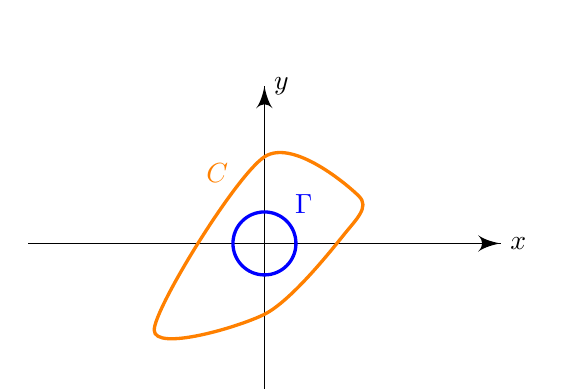
\begin{tikzpicture}[scale=1]
    % Draw x-axis
    \draw[->] (-3, 0) -- (3, 0) node[right] {$x$};
    \draw[->] (0, -2) -- (0, 2) node[right] {$y$};

    \draw[very thick, blue] (0,0) circle (0.4);
    \draw[very thick, orange] plot [smooth cycle] coordinates {(-1.4, -1.1) (0, -0.9) (1, 0.1) (1.2,0.6) (0, 1.1)};
    \node [blue] at (0.5, 0.5) {$\Gamma$};
    \node [orange] at (-0.6, 0.9) {$C$};
  \end{tikzpicture}
\end{center}
We denote by $\Omega$ the set bounded by $\Gamma$ and $C$.
If we orient $\Omega$ and $\Gamma$ counterclockwise,
then if we recall \Cref{rmk:natural-orientation},
we would get that $\partial \Omega = C + \Gamma^{-} = C - \Gamma$,
where $\Gamma^{-}$ is $\Gamma$ with the opposite orientation.
Once again, let
\[
  \omega := -\frac{y}{x^2 + y^2} \dx + \frac{x}{x^2 + y^2} \dy.
\]
Now, $\omega$ is smooth everywhere on $\Omega$,
so by exactness (in particular closedness) of $\omega$,
by Green's theorem we get that
\[
  0 =
  \int_{\Omega} \dif \omega =
  \int_{\partial \Omega} \omega
  \int_{C} \omega - \int_{\Gamma} \omega.
\]
This implies that
\[
  \int_{C} \omega = \int_{\Gamma} \omega = 2\pi,
\]
where the last equality can be computed easily by definition,
in a similar manner to what we saw in \Cref{exmp:famous-form}.
By linearity of the integral over paths, we easily obtain that
for a path $C_n$ that winds around the origin $n$ times,
we have $\int_{C_n} \omega = 2\pi n$,
and similarly if $\widetilde C$ is a path that winds around the origin
once in each direction,
we would get $\int_{\widetilde C} \omega = 2\pi - 2\pi = 0$.

\begin{definition}[Winding number]
  Let $C$ be a smooth closed curve on $\R^2 \setminus 0$,
  the winding number (or index) of $C$ is given by
  \[
    \Ind(C) :=
    \frac{1}{2\pi} \int_{C} \omega =
    \frac{1}{2\pi} \int_{C} -\frac{y}{x^2 + y^2} \dx + \frac{x}{x^2 + y^2} \dy.
  \]
  Intuitively, it's the number of times $C$ winds around the origin
  counterclockwise.
\end{definition}

\begin{remark}
  This result is very important in complex analysis.
\end{remark}

\subsection{Orientation}
\label{ssec:orientation-and-flux}
First recall the definition for a parameterized smooth surface.

\begin{definition}[Parameterized smooth surface]
  Let $U \subset \R^2$ be a bounded open set,
  and let $g \colon U \to \R^n$ be an injective smooth map with
  $\rank \Dif g(a) = 2$ for all $a \in U$.
  Then we call $S = g(U)$ a parameterized smooth surface of dimension $n$.
  In particular, it is a $2$-dimensional manifold in $\R^n$.
\end{definition}

Remember \Cref{rmk:orienation-reversing}?
It is finally time to properly define orientation.

\begin{definition}[Volume form]
  A volume form (or a top-dimensional form) is a differential form
  $\omega \in \Omega^n(M)$ of degree $n = \dim M$.
\end{definition}
\begin{remark}
  A top-dimensional form is called a volume form since it is the only
  type of form that allows us to compute the volume in the dimension
  of the manifold.
\end{remark}

\begin{definition}[Orientation via forms]
  \label{def:orientation-via-forms}
  An orientation of a smooth manfiold $M$ of dimension $n$ is
  a smooth volume form $\omega \in \Omega^n(M)$ with $\omega(p) \neq 0$
  for all $p \in M$ up to multiplication by a positive function
  $f \colon M \to \R^+$.
\end{definition}

\begin{remark}[Oriented manifold]
  A manifold is said to be orientable if it has some orientation.
  A manifold with a choice of orientation is called an oriented manifold.
  If $M$ is a connected, orientable manifold, then it has exactly two
  possible orientations,
  because the space $\bigwedge^{\!k}(T^*_p M)$ is one dimensional and since
  the orientation is not zero it must be either in the positive
  side of the vector space or in its negative side,
  and the equivalence relation makes any two forms on the same side
  equivalent as orientations.
\end{remark}

\begin{definition}[Standard orientation]
  \label{def:standard-orientation}
  The standard volume form on $\R^n$ is
  $\omega = \dx_1 \wedge \cdots \wedge \dx_n$.
  When $n \le 3$ we sometimes write $\omega = \dx \wedge \dy$
  or $\omega = \dx \wedge \dy \wedge \dz$ instead respectively.
\end{definition}

\begin{example}
  \label{exmp:orientation-of-S-one}
  Consider the unit circle $S^1 := C_1(0) \subset \R^2$.
  A volume form on $S^1$ is a $1$-form,
  for example $\omega = -y \dx + x \dy$.
  Since $\omega$ is nowhere-vanishing and smooth,
  it is an example of an orientation on $S^1$.
\end{example}

\begin{definition}[Positivity of an ordered basis]
  \label{def:std-orientation-of-a-basis}
  Let $M$ be an $n$-dimensional manifold,
  let $B = \langle v_1,v_2,\dots,v_n\rangle \subset \R^n$ be an ordered basis
  for $T_p(M)$,
  and let $\omega$ be a nowhere vanishing volume form (an orientation) on $M$.
  We say that $B = \langle v_1,v_2,\dots,v_n\rangle$ is positive with respect
  to $\omega$ if $\omega(p)(v_1,v_2,\dots,v_n) > 0$,
  and otherwise we say that it is negative with respect to $\omega$.
\end{definition}

\begin{remark}
  Note that a \textit{choice of orientation} $\omega$ on a manifold $M$,
  is equivalent to a choice of an equivalence class of
  the nowhere vanishing forms in $\Omega^n(M) / \sim$
  where $\omega \sim \tilde \omega$ if there exists
  a smooth function $f \colon M \to \R_{>0}$
  such that $\omega = f \tilde \omega$.
  By a nowhere vanishing form
  we mean that $\omega$ is not identically $0$ at any $p \in M$,
  and by equivalent, we mean that the postivity, or signs
  of ordered bases any every $p$ would be the same with respect to
  any volume form in the same equivalency class.
\end{remark}

\begin{example}
  In $\R^2$, with respect to the standard orientation,
  the standard basis $\langle e_1,e_2 \rangle$ has positive
  orientation, $\langle e_2,e_1 \rangle$ has negative orientation,
  and $\langle e_1 + e_2,e_2 \rangle$ has positive orientation.
  We can see this quickly by recalling that $\dx \wedge \dy = \det$.
\end{example}

\begin{remark}
  In \Cref{exmp:orientation-of-S-one},
  the orientation on the unit circle $S^1$ was $\omega = -y \dx + x \dy$.
  Define $g(\theta) = (\cos\theta,\sin\theta)$
  so have that $T_{g(\theta)} = t(-\sin\theta,\cos\theta)$.
  Therefore $\langle (-\sin\theta,\cos\theta) \rangle$ is an ordered
  basis for $T_{g(\theta)}$.
  With respect to the orientation $\omega$ we notice that
  $\omega_{g(\theta)}(-\sin\theta,\cos\theta) = 1$,
  and thus the direction $(-\sin\theta,\cos\theta)$ is the positive
  direction of the tangent space.
  This orientation of the tangent space tells us intuitively,
  that the orientation $\omega$ on $S^1$ is the counterclockwise orientation.
\end{remark}

\begin{definition}[Framing]
  \label{def:framing}
  A framing of a smooth manifold $M$ of dimension $n$ is a continuous function
  that sends each point on the manifold $p \in M$ to an ordered basis
  $\langle v_1(p),v_2(p),\dots,v_n(p) \rangle$
  of the tangent space $T_p(M)$.
\end{definition}
\begin{definition}[Parallelizable manifold]
  A manifold that admits a framing, is called a parallelizable manifold.
\end{definition}
\begin{example}
  The space $S^1$ from \Cref{exmp:orientation-of-S-one}
  has the framing $v_1(\theta) = \langle (-\sin\theta,\cos\theta) \rangle$,
  and therefore $S^1$ is a parallelizable manifold.
  However, $S^2 := \set{x \in \R^3 \mid \norm{x} = 1}$ is not parallelizable
  since if $v = (v_1,v_2)$ were a framing,
  then the vector field $v_1$ is a contradiction to the hairy ball theorem.
\end{example}

\begin{proposition}[Parallelizable implies orientable]
  \label{prop:parallelizable-implies-orientable}
  Every parallelizable manifold is orientable.
\end{proposition}
\begin{proof}
  Let $v = (v_1,\dots,v_n)$ be a framing on an $n$-dimensional manifold $M$.
  For every $p \in M$ define
  \[
    \omega_p(v(p)) := 1,
  \]
  and extend $\omega_p$ uniquely to an alternating multilinear volume form
  (this can be done since $\dim(\bigwedge^{\!k}(T_p M)^*) = 1$).
  Since $v$ is smooth, $\omega$ is smooth,
  and since $\omega_p(v(p)) = 1$ for all $p \in M$,
  the volume form $\omega$ is nowhere vanishing.
  Therefore $M$ is orientable which completes the proof.
\end{proof}

% \begin{remark}
%   \label{rmk:equivalency-of-orientations}
%   Recall that given an orientation via a form $\omega$,
%   and an ordered basis $\langle v_1,\dots,v_n\rangle$ for $T_p(M)$,
%   we can tell whether it is positive or not by checking
%   the sign of $\omega(v_1,\dots,v_n)$.
%   However quite surprisingly when declaring which bases are positive
%   in each tangent space in a certain smooth sense, we also get an orientation,
%   and these conditions are equivalent.
%   This won't be very relevant to our discussion,
%   so just remember that the weaker statement,
%   that every parallelizable manifold is orientable.
% \end{remark}

\begin{remark}
  By \Cref{prop:parallelizable-implies-orientable},
  all parallelizable manifolds are orientable,
  however the converse is not always true.
  For example, the $2$-sphere
  given by $S^2 = \set{p \in \R^3 \mid \norm{p} = 1}$
  is orientable,
  but by a theorem (the hairy ball theorem),
  it does not admit a framing, so it is not parallelizable.
\end{remark}

\begin{definition}[Sign of an oriented manifold]
  Let $M$ be an oriented manifold,
  let $\eta$ be a reference orientation,
  and let $\omega$ be a volume form in its choice of orientation.
  Then we define the sign of $M$ to be
  \[
    \sgn(M) :=
    \begin{cases}
      1 &\omega(p)(v_1,\dots,v_n) > 0, \\
      -1 &\omega(p)(v_1,\dots,v_n) < 0,
    \end{cases}
  \]
  for any arbitrary oriented basis $\langle v_1,\dots,v_n\rangle$
  with positive orientation with respect to $\eta$.
\end{definition}

\begin{example}
  Not all smooth surfaces are orientable.
  A M\"obius strip is not orientable.
  In topology we even say that a surface is orientable if it does not
  admit an embedding of a M\"obius strip in it.

  We will show that the M\"obius strip is not orientable.
  Let $M = [0,2\pi] \times (-1,1) / \sim$ with $(x,y) \sim (x + 2\pi,-y)$
  be the M\"obius strip,
  and assume, by way of contradiction,
  that there exists a nowhere vanishing volume form
  $\omega(x,y) = f(x,y) \dx \wedge \dy \in \Omega^2(M)$.
  Consider the map $g \colon (x,y) \mapsto (x + 2\pi,-y)$.
  We have that
  \[
    g^*(\dx \wedge \dy) =
    \dif(x + 2\pi) \wedge \dif(-y) =
    \dx \wedge (-\dy) = -\dx \wedge \dy,
  \]
  so we can compute that
  \[
    g^*(f(x,y) \dx \wedge \dy) =
    f(x + 2\pi,-y) g^*(\dx \wedge \dy) =
    -f(x + 2\pi,-y) \dx \wedge \dy,
  \]
  so for a fixed point $(0,y)$ we have
  $g^*(f(0,y) \dx \wedge \dy) = -f(2\pi,-y) \dx \wedge \dy$.
  However, since $(0,y) \sim (2\pi,-y)$,
  we must have $g^*\omega(0,y) = \omega(2\pi,-y) = \omega(0,y)$,
  and thus $g^*(f(0,y) \dx \wedge \dy) = f(0,y) \dx \wedge \dy$.
  Therefore we obtained $f(0,y) = -f(2\pi,-y)$,
  but by the equivalence $f(0,y) = f(2\pi,-y)$,
  and therefore $f(0,y) = 0$, which is a contradiction,
  which completes the proof.
\end{example}

\begin{remark}[Orientation and normal vectors]
  \label{rmk:orientation-in-surfaces}
  Let $S$ be a parallelizable surface in $\R^n$,
  and let $v = (v_1,v_2)$ be some framing function on $S$.
  We know that $v_1(p) \times v_2(p)$ is a vector orthogonal to
  the tangent space $T_p(S)$.
  Since $v_1$ and $v_2$ are continuous functions,
  the function of the unit normal vector
  $n(p) = \frac{v_1(p) \times v_2(p)}{\norm{v_1(p) \times v_2(p)}}$
  is a continuous function as a composition of continuous functions,
  and by its construction, it is completely independent of
  the choice of the framing,
  only on its sign (whether it is positive or negative),
  and in fact if the orientation had a different sign,
  then its unit normal vector function would be $\tilde n(p) = -n(p)$.
  It follows that $\sgn(S)$ has a one to one correspondence with
  the direction of the choice of a unit normal vector function.
  This also works in manifolds of higher dimensions when
  we generalize the vector product, and we could talk about it
  more when we will introduce the Hodge star operator.
  Note that even for manifolds that are not parallelizable like $S^2$,
  there is a similar normal vector at every point.
\end{remark}

\begin{example}[Framings and orientations]
  Recall that a a framing
  maps each point $p$ on a surface $S$ to an ordered basis
  $\langle v_1(p),v_2(p) \rangle$ of the tangent space of $S$ at $p$.
  The standard framing is given by mapping each point
  to the standard basis of the tangent space at that point.
  Each framing $\langle v_1(p),v_2(p) \rangle$ corresponds
  to an orientation $\omega = v_1(p) \wedge v_2(p)$.
  For example for $S = \set{(x,y) \mid x^2 + y^2 \le 1} \subset \R^2$,
  the standard framing is the constant function
  $f \colon p \mapsto \langle \dx,\dy \rangle$.
  It corresponds to the standard volume form $\omega = \dx \wedge \dy$.
\end{example}

\begin{definition}[Signed integration]
  Let $\Omega$ be a manifold with a choice of orientation,
  and let $f \colon \Omega \to \R$.
  We define:
  \[
    \int_{\Omega} f \dx_1 \wedge \cdots \wedge \dx_n =
    \sgn(\Omega) \int_{\Omega} f \dV,
  \]
  where $\sgn(\Omega)$ is taken with respect to the standard orientation
  on $\Omega$.
\end{definition}

\subsection{The interior product and induced orientation}
\label{subsec:induced-orientation}
\begin{definition}[Interior product]
  Let $M$ be a manifold,
  let $\omega \in \Omega^k(M)$,
  and let $X$ be a vector field on $M$.
  Then the interior product (sometimes called a contraction,
  or interior derivative) of $X$ is the map
  $\iota_X \colon \Omega^k(M) \to \Omega^{k-1}(M)$,
  defined by
  \[
    (\iota_X \omega)\del{X_1,\dots,X_{p-1}} =
    \omega \del{X,X_1,\dots,X_{p-1}}.
  \]
  When $\omega$ is a $0$-form,
  we define $\iota_X \omega = 0$ by convention.
\end{definition}
\begin{example}
  Let $\omega \in \Omega^1(M)$ be a $1$-form,
  and let $X \colon M \to \R^{\dim M}$ be a vector field on $M$.
  Then we get
  \[
    (\iota_X \omega) = \alpha(X) \in \Omega^0(M).
  \]
  Note that $\alpha(X) \colon M \to \R$ by $p \mapsto \alpha(X(p))$.
  Therefore, indeed $\alpha(X) \in \Omega^0(M) = C^{\infty}(M,\R)$
  (in the smooth case).
\end{example}
\begin{remark}
  Let $\omega \in \Omega^p(M)$ and $\eta \in \Omega^q(M)$.
  Then
  \[
    \iota_X(\omega \wedge \eta) =
    (\iota_X \omega) \wedge \eta + (-1)^p \omega \wedge (\iota_X \eta).
  \]
  This means that the interior derivative $\iota_X$,
  must like the exterior derivative,
  also satisfies the graded Leibniz rule
  (incidentally, this is why we call $\iota_X$
  the interior \textit{derivative}.
  It satisfies the rule of differentiation of a product).
\end{remark}

Given an orientation (nowhere vanishing volume form) $\omega \in \Omega^n(M)$
on an $n$-dimensional manifold $M$,
we want to find the induced orientation on submanifolds $N$ of 
codimension $1$ ($\dim N = n - 1$) of $M$
(in particular we are interested in the induced orientation on $\partial M$).
Therefore, we need to find the right nowhere vanishing $(n-1)$-form
on $\partial M$.
Now that we have the definition of the interior product in hand,
this is equivalent to finding the right vector field
$X \colon \partial M \to TM$,
such that if $B_p$ is a basis for $T_p \partial M$,
then $\set{X(p)} \cup B_p$ is a basis for $T_p M$.
In that case, we could define $\tilde \omega = \iota_X(\omega)$
to be the induced orientation on $\partial M$.

\begin{definition}[Outward/Inward pointing vector]
  Let $p \in \partial M$.
  We then have the inclusion $T_p \partial M \subseteq T_p M$.
  If $X_p \in T_p M$, then we can write
  \[
    X_p = \sum_{i=1}^{n} a_i e_i,
  \]
  for $a_i \in \R$ and $\langle e_1,\dots,e_{n-1} \rangle$
  an oriented basis for $T_p \partial M$, and $e_n$ an orthogonal
  complement for $T_p \partial M$ in $T_p M$,
  so that $M$ is given locally with coordinates $x_n \geq 0$.
  We say that $X_p$ is outward pointing if $a_n < 0$,
  and inward pointing if $a_n > 0$.
\end{definition}

\begin{example}
  In the unit disc $\D \subset \R^2$ with the standard orientation
  $\omega = \dx \wedge \dy$,
\end{example}

\begin{definition}[Generalized vector product]
  Let $v_1,\dots,v_{n-1}$ be vectors in $\R^n$.
  We define the generalized vector product
  $N = v_1 \times v_2 \times \cdots \times v_{n-1}$ to be the unique
  vector in $\R^n$ so that for all $x \in \R^n$ we have
  \[
    \ip{N}{x} =
    \det
    \begin{pmatrix}
      \vert & \vert & & \vert \\
      x & v_1 & \cdots & v_{n-1} \\
      \vert & \vert & & \vert \\
    \end{pmatrix}.
  \]
\end{definition}

\begin{remark}
  It can be shown that if $\langle \dx_1,\dots,\dx_{n-1} \rangle$
  is an oriented basis for $T_p \partial M$,
  then
  $\tilde N(p) = \dx_1 \times \cdots \times \dx_{n-1}$ is an outward pointing
  normal vector to $T_p \partial M$.
  We can now define the vector field
  $N \colon \partial M \to TM$
  by $N(p) = \frac{\tilde N(p)}{\norm{\tilde N(p)}}$.
  This is the generalization to
  the unit normal vector function in \Cref{rmk:orientation-in-surfaces}.
\end{remark}

\begin{definition}[Induced orientation]
  Let $M$ be an oriented manifold with boundary,
  and let $\omega$ be a nowhere-vanishing volume form defining the
  orientation of $M$.
  For $p \in \partial M$ let $N(p)$ denote the outward-pointing unit
  normal vector at $p$.
  We say that an $(n-1)$-form $\eta$ defines
  the \textit{induced orientation} on $\partial M$
  if for any $e_1,\dots,e_{n-1} \in T_p \partial M$
  so that $\langle e_1,\dots,e_{n-1} \rangle$ is an oriented basis
  for $T_p \partial M$ we have,
  \[
    \eta(p)(e_1,\dots,e_{n-1}) = \omega(p)(N(p),e_1,\dots,e_{n-1}).
  \]
  That is, $\eta = \iota_N \omega$.
\end{definition}

\begin{example}
  \label{exm:induced-orientation}
  Let $M = \set{(x,y) \in \R^2 \mid x^2 + y^2 \le 1}$,
  so that $\partial M = S^1$ is the unit circle.
  Give $M$ the standard orientation via the volume form
  $\omega = \dx \wedge \dy$, so in particular $\sgn(M) = 1$.
  Now we want to find the orientation of $\partial M$ induced by $M$.
  First, we can compute and quickly and
  find that $N(p) = (\cos\theta,\sin\theta)$ is the outward pointing
  vector at each $p \in \partial M$ where $\theta$ is the angle
  between $p$ and the $x$ axis.
  The induced orientation is thus $\iota_N \omega$.
  We can now compute and get that for $v \in \R^2$,
  \[
    (\iota_N \omega)(p)(v) =
    \omega(p)(N(p),v)  =
    \det(N(p) \mid v) =
    \cos\theta v_y - \sin\theta v_x,
  \]
  so the induced orientation is
  $\tilde \omega = -\sin\theta \dx + \cos\theta \dy$.
  In polar coordinates we get
  \[
    \tilde \omega =
    -\sin\theta \dif(\cos\theta) + \cos\theta \dif(\sin\theta) =
    (-\sin\theta)^2 \dtheta + (\cos\theta)^2 \dtheta = \dtheta.
  \]
  Let $\gamma(t) = (1,t)$ be a parameterization
  for the circle in polar coordinates so that
  $\langle\gamma'(t)\rangle = \langle(0,1)\rangle$
  is an oriented basis for $T_p \partial M$ at any point $p \in \partial M$.
  We get that $\dtheta(\gamma'(t)) = 1 > 0$,
  and therefore the basis $\langle\gamma'(t)\rangle$ has positive
  orientation.
  This implies that $\gamma'(t)$ has positive orientation,
  and in paritucular, the orientation is counterclockwise.
  This coincides with the natural induced orientation for the boundary
  we introduced in \Cref{def:natural-induced-orientation}.
  If our reference form for the sign of $\partial M$
  is $\eta = \dtheta$, then clearly $\sgn(\partial M) = 1$,
  and if $\eta = -\dtheta$ then $\sgn(\partial M) = -1$.
\end{example}

\begin{exercise}
  Show that the induced orientation on $\partial \R^k_+$ is the usual one
  on $\R^{k-1}$ if and only if $k$ is even.
\end{exercise}

\begin{remark}
  When first stating Green's theorem we used the definition
  of ``natural orientation''.
  However, as we saw in \Cref{exm:induced-orientation},
  we can simply use the more general definition of induced orientation instead.
  Computationally, this does not change a thing,
  but mathematically, this implies there may be a way to generalize
  Green's theorem to higher dimensions.
\end{remark}

\begin{definition}[Flux]
  Let $S \subset \R^3$ be an oriented surface,
  let $\vec F = (F_1,F_2,F_3)$ be a continuous vector field,
  and let
  $\omega = F_1 \dy \wedge \dz + F_2 \dz \wedge \dx + F_3 \dx \wedge \dy$
  be the flux form associated with $\vec F$.
  Suppose that $g \colon \Omega \to S$ is a smooth parameterization of $S$.
  Then the flux $\Phi$ of $\vec F$ across $S$ is defined to be:
  \[
    \int_{S} \omega =
    \int_{\Omega} g^*\omega =
    \int_{\Omega} \ip{\vec F(g(u,v))}{\frac{g'_u \times g'_v}{\norm{g'_u \times g'_v}}} \norm{g'_u \times g'_v} \du \wedge \dv =
    \int_{\Omega} \left\langle 
    \vec F(g(u,v)), g'_u \times g'_v \right\rangle \du \dv
  \]
\end{definition}

\begin{remark}
  \label{rmk:surface-area-element-pullback-discovery}
  Recall that we also described $\Phi$
  by $\int_{S} \ip{\vec F}{\vec n(u,v)} \dsigma$,
  where $\dsigma$ is the \textit{surface area element}.
  We now understand that $\dsigma$ is the differential
  form that satifies that its pullback is equal to the form
  $g^*(\dsigma) = \norm{g'_u \times g'_v} \du \wedge \dv$.
\end{remark}

\begin{exercise}
  Let $S$ be the orientable surface given by
  \[
    S := \set{(x,y,z) \bmid z \geq 0 \stand z = 4 - x^2 - y^2}.
  \]
  Compute the flux of the field $\vec F(x,y,z) = (xz, yz, x^2 + y^2)$
  across $S$,
  where $S$ is given the induced orientation as the boundary of
  the area bounded between $S$ and the plane $z = 0$.
  Equivalently, it is given the orientation by declaring that
  an ordered basis $\langle v_1,v_2\rangle$ of its tangent space,
  is positive if and only if $\langle n(p),v_1,v_2\rangle$ is a positive
  basis for $\R^3$ where $n(p)$ is the outward pointing unit normal vector
  at $p \in S$.
\end{exercise}
\begin{solution}
  In order to calculate this integral we first need to find a
  parameterization to this surface,
  for example $g \colon \Omega \to \R^3$ where
  \[
    \Omega := \set{(u,v) \in \R^2 \mid u^2 + v^2 \le 4} \quad
    g(u,v) := (u,v,4-u^2-v^2)
  \]
  Recall that
  \[
    \Phi := \int_{S} \omega =
    \int_{\Omega} \left\langle 
    \vec F(g(u,v)), g'_u \times g'_v \right\rangle \du \dv,
  \]
  where the order $g'_u \times g'_v$ (and not $g'_v \times g'_u$)
  was chosen because it is the order that gives an outward pointing normal.
  By a simple computation:
  \[
    g_u =
    \begin{pmatrix}
      1 \\ 0 \\ -2u
    \end{pmatrix} \tand
    g_v =
    \begin{pmatrix}
      0 \\ 1 \\ -2v
    \end{pmatrix},
  \]
  and thus
  \[
    g_u \times g_v =
    \hat x
    \begin{vmatrix}
      0 & 1 \\
      -2u & 2v
    \end{vmatrix} +
    \hat y
    \begin{vmatrix}
      -2u & -2v \\
      1 & 0
    \end{vmatrix} +
    \hat z
    \begin{vmatrix}
      1 & 0 \\
      0 & 1
    \end{vmatrix} = \cdots =
    \begin{pmatrix}
      2u \\ 2v \\ 1
    \end{pmatrix}.
  \]
  We can now plug in the values:
  \begin{small}
  \begin{align*}
    \int_{\Omega}
    \vec F\del{g(u,v)} \cdot (g_u \times g_v) \du \wedge \dv &=
    \iint_{\Omega}
    \left[u (4 - u^2 - v^2),v (4 - u^2 - v^2),u^2 + v^2\right] \cdot
    \left[2u,2v,1\right]^T \du \dv \\ &=
    \iint_{\Omega} (u^2 + v^2) \left[2 (4 - u^2 - v^2) + 1\right] \du \dv
                                  \\&=
    \int_{0}^{2\pi} \int_{0}^{2} (9r^2 - 2r^4) r \dr \dtheta.
  \end{align*}
  \end{small}

  \noindent where the last transition is the change of variables theorem.
  The computation of the last integral is very basic,
  so we will omit it and conclude the exercise here.
\end{solution}

\subsection{Surface area element}
The purpose of this short subsection is to understand what is the
surface area element discussed in
\Cref{rmk:surface-area-element-first-discovery},
\Cref{rmk:surface-area-element-second-discovery}, and
\Cref{rmk:surface-area-element-pullback-discovery}.

\begin{remark}[Geometric interpretation of the interior product]
  Recall that the interior product takes a $k$-form $\omega$,
  a vector field $X$ and returns a $(k-1)$-form $\iota_X \omega$
  which is simply $\omega$ with $X$ inserted in its first argument.
  
  Recall that when $\omega$ is a volume form ($\omega \in \Omega^n(M)$),
  it computes the $n$-dimensional volume of the parallelopiped spanned by
  $n$ vectors in $\R^n$.

  In this case,
  the geometrical interpretation of $\iota_X \omega$ at a point $p$
  is that it computes the $n$-dimensional volume of the parallelopiped spanned
  by $X(p)$ and $n-1$ other vectors in $\R^n$.

  We claim that that this value is equal to the $(n-1)$-dimensional
  volume of the parallelopiped spanned by $n-1$ vectors in $\R^n$
  projected onto the affine space that is orthogonal complement of $X(p)$
  at $p$, or in other words projected onto the tangent space $T_p(M)$.
  This is the reason the interior product is sometimes called a ``contraction''.
\end{remark}

\begin{example}
  The simplest example is to consider the area form $\omega = \dx \wedge \dy$,
  and the constant vector field $X(\vec p) \equiv (1,0)$
  for all $\vec p \in \R^2$.
  In this case we have
  \[
    \iota_X\omega(\vec p)(\vec v) =
    \det
    \begin{pmatrix}
      1 & v_x \\
      0 & v_y
    \end{pmatrix} =
    v_y,
  \]
  for all $\vec v = (v_x,v_y) \in \R^2$.
  This implies clearly that $\iota_X\omega = \dy$,
  which coincides with the previously discussed geometric interpretation
  of the interior product.
\end{example}

\begin{remark}
  Consider the manifold $M = S^2$
  endowed with the standard orientation induced by $\R^3$,
  which is $\eta := \iota_N(\dx \wedge \dy \wedge \dz)$ where $N$ is the vector
  field that assigns each $p \in S^2$ an outward pointing normal vector,
  we get that $\eta$ is the standard area form on $T_p(S^2)$.
  The form $\eta$ is exactly what we need in order to integrate
  some any function over $S^2$.
  This is true in general for any oriented manifold $M$.
  When $M$ is a curve,
  the form $\eta$ is called the \textit{curve length element}
  associated with $M$.
  When $M$ is a surface,
  the form $\eta$ is called the \textit{surface area element}
  associated with $M$.
\end{remark}

\begin{example}
  Let $C$ be a $1$-dimensional oriented curve in $\R^2$,
  and let $\eta = \iota_N(\omega) \in \Omega^1(C)$ be its curve length element,
  where $\omega = \dx \wedge \dy$ is the standard volume form on $\R^2$.
  Let $\gamma(t) = (x(t),y(t))$ be a local parameterization of $C$,
  and write $\eta$ explicitly $\eta = N_x \dy - N_y \dx$,
  where $N$ is the outward pointing normal ($\omega(N,\gamma') > 0$).
  Notice that we can write $N$ explicitly by rotating the
  vector $\gamma'(t) = (x'(t),y'(t))$ and normalizing as follows:
  \[
    N(t) =
    \frac{(y'(t), -x'(t))}{\sqrt{\del{x'(t)}^2 + \del{y'(t)}^2}}.
  \]
  This means that we can compute the pullback
  of the functions $N_x(x,y)$ and $N_y(x,y)$ easily and get
  \[
    \gamma^*\eta(t) =
    \frac{y'(t)}{\sqrt{\del{x'(t)}^2 + \del{y'(t)}^2}} \gamma^*\dy -
    \frac{-x'(t)}{\sqrt{\del{x'(t)}^2 + \del{y'(t)}^2}} \gamma^*\dx =
    \frac{x'(t) \gamma^*\dx + y'(t) \gamma^*\dy}{\sqrt{\del{x'(t)}^2 + \del{y'(t)}^2}}.
  \]
  Note that $\dif x(t) = x'(t) \dt$ and $\dif y(t) = y'(t) \dt$,
  so we get that
  \[
    \gamma^*\eta(t) =
    \frac{x'(t) \gamma^*\dx + y'(t) \gamma^*\dy}{\sqrt{\del{x'(t)}^2 + \del{y'(t)}^2}} =
    \frac{x'(t) x'(t) \dt + y'(t) y'(t) \dt}{\sqrt{\del{x'(t)}^2 + \del{y'(t)}^2}} =
    \sqrt{\del{x'(t)}^2 + \del{y'(t)}^2} \dt
  \]
  Recall that $\norm{\gamma'(t)} = \sqrt{\del{x'(t)}^2 + \del{y'(t)}^2}$,
  and therefore the curve length element is
  \[
    \gamma^*\eta = \norm{\gamma'(t)} \dt.
  \]
  Compare this result with \Cref{rmk:curve-length-element}.
\end{example}

\begin{example}
  Let $S$ be a $2$-dimensional oriented surface,
  and let $\eta = \iota_N(\omega)$ be its surface area element.
  Let $g \colon U \to \R^3$ be a local parameterization of $S$,
  so that $g(u,v) = (x(u,v),y(u,v),z(u,v))$,
  and write $\eta$ explicity $\eta = N_x \dy \wedge \dz + N_y \dz \wedge \dx + N_z \dx \wedge \dy$.
  Using the notation $\partial_u$ and $\partial_v$ for the basis tangent vectors
  of $T_{(u,v)}(U)$, by definition of the pullback we get that
  \[
    g^*\eta_{(u,v)}(\partial_u,\partial_v) =
    \eta_{g(u,v)}(\dif g_{(u,v)}(\partial_u),\dif g_{(u,v)}(\partial_v)) =
    \eta(g_u,g_v),
  \]
  and so by definition of $\eta$ we get
  $g^*\eta(\partial_u,\partial_v) = \omega(N,g_u,g_v)$,
  however since $N(u,v) = \frac{g_u \times g_v}{\norm{g_v \times g_v}}$,
  we can compute that
  \[
    \omega(N,g_u,g_v) =
    \frac{1}{\norm{g_u \times g_v}}
    \det
    \begin{pmatrix}
      \vert & \vert & \vert \\
      g_u \times g_v & g_u & g_v \\
      \vert & \vert & \vert
    \end{pmatrix} =
    \frac{\norm{g_u \times g_v}^2}{\norm{g_u \times g_v}} =
    \norm{g_u \times g_v}.
  \]
  Since $g^*\eta(\partial_u,\partial_v) = \norm{g_u \times g_v}$,
  we can expand $g^*\eta$ multilinearly and antisymmetrically,
  and get that $g^*\eta = \norm{g_u \times g_v} \du \wedge \dv$.
  Compare this with \Cref{rmk:surface-area-element-first-discovery}.
\end{example}

\newpage

\section{Generalized Stokes theorem}

\subsection{Partition of unity}
So far we know how to integrate a $k$-form over a parameterized
$k$-dimensional manifold by pulling back.
In general, a manifold will be a union of parametrized pieces that overlap,
and so summing the integrals will give a meaningless result.
In this subsection, we will introduce a tool that will help us
overcome this challenge by partitioning the global integration problem
into local ones.

\begin{definition}[Smooth manifold with boundary]
  \label{def:smooth-manifold-with-boundary}
  A subset $M \subset \R^n$ is called a smooth $k$-manifold 
  with boundary of dimension $k$ if for every $p \in M$ there exists
  a neighbourhood $p \in U$, an open set $V \subset \R^k$ and
  an injection $H \in C^{\infty}(V, \R^n)$ such that:
  \begin{enumerate}
    \item[(1)] $\rank \Dif H(v) = k$ for all $v \in V$.
    \item[(2)] $M \cap U = H(V \cap \mathcal{H}_k)$.
    \item[(3)] $H^{-1} \colon M \cap U \to V \cap \mathcal{H}_k$
    is continuous with respect to the topology induced by $\R^n$.
  \end{enumerate}
  In other words, $H$ restricts to a homeomorphism
  $H \colon V \cap \mathcal H_k \to M \cap U$.
  The function $H$ is called a \textit{parametrization},
  or a \textit{chart} of $M$ at $p$.
  Indeed, we also require charts to be compatible,
  that is,
  if there exist $H_i \colon V_i \to \R^n$ and $H_j \colon V_j \to \R^n$
  which overlap, then we require the \textit{transition map}
  $H_i^{-1} \circ H_j$ to be smooth.
  We say that $p \in \partial M$ if $p = H(u)$ for some
  $u \in \mathcal H_k$.
\end{definition}
\begin{remark}
  In \Cref{def:smooth-manifold-with-boundary},
  $H(V)$ is sometimes called a \textit{coordinate chart} on $M$,
  and a \textit{coordinate ball} on $M$ is the image of some ball
  under some parameterization $H$.
\end{remark}

\begin{theorem}[Partition of unity]
  \label{thm:partition-of-unity}
  Let $M \subset \R^n$ be a compact $k$-dimensional manifold with boundary.
  Then there are smooth real-valued functions
  $\varphi_1,\dots,\varphi_N$ on $M$ so that:
  \begin{enumerate}
    \item[(1)] $0 \le \varphi_i \le 1$ for all $1 \le i \le N$.
    \item[(2)] Each $\varphi_i$ is zero outside some coordinate ball.
    \item[(3)] $\sum_{i=1}^{N} \varphi_i \equiv 1$.
  \end{enumerate}
\end{theorem}
\begin{remark}
  We call $\set{\varphi_i}$ a \textit{partition of unity} on $M$.
\end{remark}

\begin{definition}[Support]
  Let $f \colon X \to Y$ be a function between
  two manifolds.
  Then the support of $f$ is defined to be the set
  \[
    \supp(f) :=
    \overline{\set{x \in X \mid f(x) \neq 0}}.
  \]
\end{definition}

\begin{definition}[Bump function]
  A function $f \colon \R^n \to \R$ that is smooth and has a compact support.
\end{definition}
\begin{remark}
  The set of all bump functions with domain $\R^n$
  forms a vector space,
  denoted by $C_0^{\infty}(\R^n)$ or $C_c^{\infty}(\R^n)$.
\end{remark}

\begin{example}
  \label{exmp:bump-function}
  First define $h \colon \R \to \R$ be
  \[
    h(x) =
    \begin{cases}
      e^{-\frac{1}{x}}, &x > 0 \\
      0, &x \le 0
    \end{cases}.
  \]
  Then we know from analysis $1$ that $h$ is smooth and all of its
  derivatives vanish at the origin.
  Next define:
  \[
    j(x) =
    \frac{\int_{0}^{x} h(t) h(1 - t) \dt}{\int_{0}^{1} h(t) h(1 - t) \dt},
  \]
  and define $\psi \colon \R^k \to \R$ by $\psi(\vec x) = j(3 - 2\norm{x})$.
  Then by a matter of technical calculation (or a particularly strong belief),
  we get that $\psi$ is a smooth function so that
  $\psi(\vec x) = 1$ for $\norm{\vec x} \le 1$ and $\psi(\vec x) = 0$ whenever
  $\norm{x} \geq 3/2$, so $\psi$ has compact support.
  Therefore $\psi$ is an example of a bump function.
\end{example}

\begin{proofof}{\Cref{thm:partition-of-unity}}
  Let $\psi$ be the bump function from \Cref{exmp:bump-function}.
  For each point $\vec p \in M$,
  choose a coordinate chart whose domain is a ball of radius $2$ in $\R^k$,
  and if $\vec p \in \partial M$ let that be the half-ball of radius $2$
  (this can be done since any open set in $\R^k$ contains an open ball,
  in particular with center $\vec p$, then by restricting the chart to
  that ball we get what we need).
  Since the images of those balls restricted to radius $1$ cover the
  manifold, and since the manifold is compact,
  there exist a finite amount of $\vec p$,
  so that their repective balls of radius $1$ 
  contained in the balls of radius $2$ denoted $V_1,\dots,V_n$,
  cover $M$.
  Let $g_i \colon B_2(0) \to V_i$ be their respective coordinate charts,
  and define $\theta_i = \psi \circ g_i^{-1}$,
  interpreting $\theta$ to be defined on all of $M$ by letting it
  be $0$ outside of $V_i$ (note that $\theta_i$ is smooth since $\psi$
  is zero outside the ball of radius $3/2$).
  Define
  \[
    \rho_i =
    \frac{\theta_i}{\sum_{j=1}^{N} \theta_j}.
  \]
  Note that for each $\vec p \in M$,
  we have $\vec p = g_j(\vec u)$ for some $j$ and $\vec u \in B_1(0)$,
  and hence $\theta_j(\vec p) = 1$ for some $j$,
  which implies that the sum is always greater than $1$ and in particular
  it does not vanish.
  If we recall the original statement, we can now notice that
  the functions $\set{\rho_i}$ form a partition of unity on $M$.
\end{proofof}

\begin{remark}
  Let $M \subset \R^n$ be a compact, oriented $k$-dimensional manifold
  (with piecewise-smooth boundary),
  let $\omega$ be a $k$-form on $M$,
  let $\set{\rho_i}$ be a parition of unity,
  and let $g_i$ be the corresponding parameterizations,
  which we take to be orientation preserving (we can do this
  because if any $g_i$ is not orientation preserving we just precompose
  it with a reflection).
  Then we define
  \[
    \int_M \omega =
    \int_M \del{\sum_{i=1}^{N} \rho_i \omega} =
    \sum_{i=1}^{N} \int_{B_2(0)} g_i^*(\rho_i \omega) =
    \sum_{i=1}^{N} \int_{B_2(0)} \psi g_i^* \omega.
  \]
  Note that we used all properties of a partition of unity in order
  for this to work.
\end{remark}

\begin{remark}
  When considering complex manifolds (manifolds with a complex structure),
  we can have a partition of unity on them only when we identity them
  as a smooth manifold.
  We cannot have a ``holomorphic partition of unity'' because
  by Liouville's theorem all holomorphic functions with compact support
  must be identically zero.
\end{remark}

\subsection{Stokes' theorem}

\begin{theorem}[Stokes' theorem]
  \label{thm:general-stokes}
  Let $k > 1$,
  and let $M$ be a compact oriented $k$-dimensional manifold in $\R^n$.
  Give $\partial M$ the induced orientation if $\partial M$ is nonempty.
  Let $\omega$ be a $k-1$ form defined in an open set of $\R^n$
  containing $M$. Then
  \[
    \int_{M} \dif \omega =
    \int_{\partial M} \omega
  \]
  if $\partial M$ is nonempty, and $\int_{M} \dif \omega = 0$ otherwise.
\end{theorem}
\begin{remark}
  Note that the usual fundamental theorem of calculus,
  the fundamental theorem of calculus for line integrals,
  and Green's theorem are all special cases of this theorem.
  The following equation shows the first example clearly:
  \[
    \int_{a}^{b} \dif f =
    \int_{a}^{b} f'(t) \dt =
    f(b) - f(a).
  \]
\end{remark}
\begin{proofof}{\Cref{thm:general-stokes}}
  to be added
\end{proofof}
\begin{remark}
  Stokes' theorem is also valid when the boundary,
  rather than being a $(k-1)$-manifold in itself,
  is piecewise smooth (when the manifold has ``corners'').
  For example, we may apply it on shapes like a closed cube,
  or a cone.
\end{remark}

\begin{corollary}
  Let $M$ be a compact oriented $k$-dimensional manifold without boundary.
  Let $\omega$ be an exact $k$-form.
  Then $\int_{M} \omega = 0$.
\end{corollary}
\begin{proof}
  Immediate.
\end{proof}

\begin{example}
  Define the smooth $2$-form:
  \[
    \omega :=
    \frac{x \dy \wedge \dz + y \dz \wedge \dx + z \dx \wedge \dy}
    {(x^2 + y^2 + z^2)^{3/2}} \in \Omega^2(\R^3 - \set{0}).
  \]
  On a sphere of radius $a$, centered at the origin,
  $\omega$ is simply $\frac{1}{a^2}$ times the standard area (volume) $2$-form.
  Suppose $g$ is the parameterization of spherical coordinates,
  then one can compute that
  \[
    g^*\omega = \sin \theta \dtheta \wedge \dvarphi.
  \]
  It is clear that $\dif(g^*\omega) = 0$,
  and since $\det \Dif g \neq 0$ whenever $\rho \neq 0$ and
  $\theta \neq 0,\pi$, it follows that $\dif \omega = 0$
  (we could have also computed this directly).
  We can now compute that for any sphere $S$ centered at the origin:
  \[
    \int_S \omega =
    \int_{0}^{2\pi} \abs{\dvarphi} \int_{0}^{\pi} \sin \theta \abs{\dtheta} =
    4\pi,
  \]
  however, for the ball $B$ associated with $S$ we get
  $\int_{B} \domega = \int_{B} 0 = 0$.
  This seems as if Stokes' theorem has failed,
  but the real reason behind this mismatch is that $\omega$ is not
  smooth (and it's not even defined) on all of $B$.
  We want to claim that
  \[
    \int_{\partial \Omega} \omega =
    \begin{cases}
      4\pi, &0 \in \Omega \\
      0, &0 \notin \Omega
    \end{cases}.
  \]
  When $0 \notin \Omega$ we can apply Stokes' theorem and immediately
  get the desired result.
  When $0 \in \Omega$, we choose $\epsilon > 0$ sufficiently small
  so that $\overline B(0,\epsilon) \subset \Omega$,
  then denote $\Omega_{\epsilon} = \Omega - B(0,\epsilon)$,
  so that $\partial \Omega_{\epsilon} = \partial \Omega - S_{\epsilon}$.
  Then $0 \notin \Omega_{\epsilon}$ so
  \[
    0 =
    \int_{\partial \Omega_{\epsilon}} \omega =
    \int_{\partial \Omega} \omega - \int_{S_{\epsilon}} \omega.
  \]
  Thus,
  \[
    \int_{\partial \Omega} \omega =
    \int_{S_{\epsilon}} \omega = 4\pi,
  \]
  as we saw earlier.
\end{example}

\newpage

\section{Applications to physics}

\subsection{Classical Stokes' theorem}

We have already seen that a vector field in $\R^3$ can be interpreted
either as a $1$-form (when we are computing work),
or as a $2$-form (when we are computing flux).
We have seen that for a function ($0$-form)
that $\dif f$ correponds to the vector field $\nabla F$,
and now we want to give the traditional interpretations of the exterior
derivative on $1$-forms and $2$-forms as well.

\begin{definition}[Curl]
  \label{def:curl}
  Let $\omega = F_1 \dx_1 + F_2 \dx_2 + F_3 \dx_3$ be a $1$-form
  on $\R^3$,
  and let $\vec F = (F_1,F_2,F_3)$ be its corresponding vector field.
  By the definition of the exterior derivative:
  \[
    \dif \omega =
    \del{\diffp{{F_3}}{{x_2}} - \diffp{{F_2}}{{x_3}}} \dx_2 \wedge \dx_3 +
    \del{\diffp{{F_1}}{{x_3}} - \diffp{{F_3}}{{x_1}}} \dx_3 \wedge \dx_1 +
    \del{\diffp{{F_2}}{{x_1}} - \diffp{{F_1}}{{x_2}}} \dx_1 \wedge \dx_2.
  \]
  The curl of $\vec F$ is defined to be the following vector field:
  \[
    \curl (\vec F) :=
    \left(
    \diffp{{F_3}}{{x_2}} - \diffp{{F_2}}{{x_3}},
    \diffp{{F_1}}{{x_3}} - \diffp{{F_3}}{{x_1}},
    \diffp{{F_2}}{{x_1}} - \diffp{{F_1}}{{x_2}}
    \right).
  \]
\end{definition}
\begin{remark}
  In older texts, it is also common to use the notation
  $\rot(\vec F)$ for $\curl(\vec F)$, where $\rot$ stands for rotor.
  Both suggest that $\curl(\vec F)$ has something to do with rotation
  (curling).
\end{remark}
\begin{remark}
  Note that the curl can also be written as
  the vector product of $\nabla$ and $\vec F$ as follows:
  \renewcommand{\arraystretch}{1.5}
  \[
    \curl(\vec F) = \nabla \times \vec F =
    \begin{vmatrix}
      \hat i & \hat j & \hat k \\
      \diffp{}{{x_1}} & \diffp{}{{x_2}} &\diffp{}{{x_3}} \\
      F_1 & F_2 & F_3
    \end{vmatrix}.
  \]
\end{remark}

\begin{remark}
  \label{rmk:curl-grad}
  Note that for all $C^2$ functions $f$ we have that
  $\curl(\grad f) = \curl(\nabla f) = 0$,
  since we know by the identity $\dif^2 = 0$ we get
  that $\dif(\dif f) = 0$.
  This is no more than a reformulation of
  \Cref{rmk:curl-of-gradient-is-zero}.
\end{remark}

\begin{theorem}[Classical Stokes' theorem]
  \label{thm:stokes}
  Let $S \subset \R^3$ be a compact, oriented surface with boundary.
  Let $\vec F$ be a smooth vector field defined on all of $S$.
  Then we have
  \[
    \int_{\partial S} \underbrace{\vec F \cdot \vec T \ds}_{\omega} =
    \int_{S} \underbrace{\curl(\vec F) \cdot \vec n \dS}_{\dif \omega},
  \]
  where $\vec T$ is the tangent unit vector,
  $\ds$ is the curve length element,
  $\vec n$ is the outward pointing unit normal vector,
  and $\dS$ is the scalar surface area element.
\end{theorem}

\begin{remark}
  Indeed, if $\omega = F_1 \dx_1 + F_2 \dx_2 + F_3 \dx_3$
  and $\gamma \colon [a,b] \to C \subset \partial S$
  is a chart of $\partial S$, we get that
  \[
    \gamma^*\del{\vec F \cdot \vec T \ds} =
    \vec F(\gamma(t)) \cdot \frac{\gamma'(t)}{\norm{\gamma'(t)}} 
      \norm{\gamma'(t)} \dt =
    \vec F(\gamma(t)) \cdot \gamma'(t) \dt =
    \gamma^*\omega,
  \]
  therefore we get that $\omega = \vec F \cdot \vec T \ds$ on
  the chart $C$, and since this holds for all charts of $\partial S$,
  which cover $\partial S$, we get that $\omega = \vec F \cdot \vec T \ds$
  on $\partial S$.
  Think about what similar argument using partition of unity could show
  that integrating over $\omega$ and $\vec F \cdot \vec T \ds$ gives
  the same result without \textit{mentioning} that they are globally equal.
  
  Similarly for a chart $(U,g)$ of $S$ we get that
  \begin{multline*}
    g^*\del{\curl(\vec F) \cdot \vec n \dS} =
    \curl(\vec F(g(u,v))) \cdot
    \frac{g'_u \times g'_v}{\norm{g'_u \times g'_v}} \norm{g'_u \times g'_v}
    \du \wedge \dv \\ =
    \curl(\vec F(g(u,v))) \cdot g'_u \times g'_v \du \wedge \dv =
    g^*\dif \omega,
  \end{multline*}
  where the last transition follows from a simple computation.
  Then we conclude in the same way
  that $\dif \omega = \curl(\vec F) \cdot \vec n \dS$ on $S$,
  and therefore the classical Stokes' theorem is indeed a special case
  of the generalized Stokes' theorem.
\end{remark}

\subsection{Geometric intuition for curl}
\label{sec:curl-intuition}
Visualize $\vec F$ as the velocity field of a fluid.
Then the line integral $\int_{C} \vec F \cdot \vec T \ds$ around a closed
curve $C$ could be interpreted as the \textit{circulation} of $\vec F$
around $C$, which we may think of as the tendency of a piece of wire
of the shape of $C$ to spin when dropped in the fluid.

\begin{example}
  Let $S = D_r$ be the $2$-dimensional disc of radius $r$ centered
  at $a$, with normal vector $\vec n$.
  Then Stokes' theorem gives us that
  \[
    \int_{\partial D_r} \vec F \cdot \vec T \ds =
    \int_{D_r} \curl(\vec F) \cdot \vec n \dS,
  \]
  and since the curl is a continuous function,
  the flux integral (note that the right hand side is a flux integral)
  satisfies the mean value theorem for integrals,
  which implies that for some $q \in D_r$ we have
  \[
    \int_{D_r} \curl(\vec F) \cdot \vec n \dS =
    \Vol(D_r) \curl(\vec F)(q) \cdot \vec n(q),
  \]
  so combined with Stokes' theorem
  \[
    \curl(\vec F)(q) \cdot \vec n(q) =
    \frac{1}{\pi r^2} \int_{\partial D_r} \vec F \cdot \vec T \ds,
  \]
  and when taking $r \to 0^+$ we get $q \to a$, and then
  \[
    \curl(\vec F)(a) \cdot \vec n(a) =
    \lim_{r \to 0^+}
    \frac{1}{\pi r^2} \int_{\partial D_r} \vec F \cdot \vec T \ds,
  \]
  so indeed the tendency to spin at $a$ is greatest when $\vec n(a)$
  is pointing in the direction of $\curl(\vec F)(a)$.
  The most common metaphor is to imagine a paddlewheel with an axle
  pointing in the direction of $\vec n(a)$.
  In this case the paddlewheel will spin the fastest when $\vec n(a)$
  points in the direction of $\curl(\vec F)(a)$.
\end{example}

\begin{remark}
  Some authors denote $\vec T \ds = \dif \vv r$ and
  $\vec n \dS = \dif \vv S$ or $\vec n \dS = \dif \vv n$.
  In these cases Stokes' theorem becomes:
  \[
    \int_{\partial S} \vec F \cdot \dif \vv r =
    \int_{S} \curl(\vec F) \cdot \dif \vv n.
  \]
  In this form we can see more clearly that Stokes' theorem simply states
  that the line integral of a vector field over a loop
  is equal to the surface integral (the flux integral)
  of its curl over the enclosed surface.
\end{remark}

\subsection{Classical divergence theorem}

\begin{definition}[Divergence]
  \label{def:div}
  Let $\omega = 
  F_1 \dx_2 \wedge \dx_3 + F_2 \dx_3 \wedge \dx_1 + F_3 \dx_1 \wedge \dx_2$
  be a $2$-form on a surface $S \subset \R^3$ written as a flux form.
  Then we have
  \[
    \dif \omega =
    \del{\frac{\partial F_1}{\partial x_1} + \frac{\partial F_2}{\partial x_2} + \frac{\partial F_3}{\partial x_3}} \dx_1 \wedge \dx_2 \wedge \dx_3.
  \]
  Correspondingly, for a vector field $\vec F = (F_1,F_2,F_3)$ we define
  its divergence to be the following scalar function:
  \[
    \div(\vec F) :=
    \frac{\partial F_1}{\partial x_1} + \frac{\partial F_2}{\partial x_2} + \frac{\partial F_3}{\partial x_3}.
  \]
\end{definition}
\begin{remark}
  \label{rmk:div-curl}
  Note that we can write $\div(\vec F) = \nabla \cdot \vec F$.
  The notation $\div$ is short for ``divergence''.
  We shall soon see what it means geometrically.
  In this case $\dif^2 = 0$ can be restated as
  $\div(\curl \vec F) = 0$ for all $C^2$ vector fields $\vec F$.
  Using divergence, the generalized Stokes' theorem takes the following form,
  sometimes called Gauss' thoerem.
\end{remark}

\begin{theorem}[Classical divergence theorem]
  Suppose $\vec F$ is a smooth vector field on a compact orientable
  $3$-manifold with boundary $\Omega \subset \R^3$.
  Then
  \[
    \int_{\partial \Omega} \underbrace{\vec F \cdot \vec n \dS}_{\omega} =
    \int_{\Omega} \underbrace{\div(\vec F) \dV}_{\dif \omega},
  \]
  where $\vec n$ is the outward pointing unit normal.
\end{theorem}
\begin{remark}
  The classical divergence theorem is sometimes called Gauss' theorem,
  or Ostrogradsky's theorem.
\end{remark}

\begin{example}
  We can use the divergence theorem to understand the relation between
  the volume of a sphere and its surface area.
  Let $B_R$ be a ball of radius $R$ around the origin.
  Let $\vec F$ be a vector field with $\vec F = \frac{1}{3} (x,y,z)$.
  We notice that
  \[
    \div(\vec F) = \nabla \cdot \vec F =
    \diffp{{F_1}}{x} +
    \diffp{{F_2}}{y} +
    \diffp{{F_3}}{z} = \frac{1}{3} + \frac{1}{3} + \frac{1}{3} = 1.
  \]
  The outward pointing
  unit normal vector to a point on the boundary of the ball
  $(x,y,z) \in \partial B_R$ is given by $\frac{1}{R} (x,y,z)$.
  Since we have that
  \[
    \Vol(B_R) =
    \int_{B_R} 1 \dV =
    \int_{B_R} \div(\vec F) \dV
  \]
  by the divergence theorem we conclude that
  \[
    \Vol(B_R) =
    \int_{\partial B_R} \vec F \cdot \vec n \dS =
    \int_{\partial B_R} \frac{1}{3R} \underbrace{(x^2 + y^2 + z^2)}_{R^2} \dS =
    \frac{R}{3} \int_{\partial B_R} 1 \dS =
    \frac{R}{3} \cdot \A(\partial B_R),
  \]
  where $\A(\partial B_R)$ is the surface area of the ball.
  This is indeed the desired result because we know that
  \[
    \A(\partial B_R) = 4 \pi R^2 \tand
    \Vol(B_R) = \frac{4 \pi R^3}{3}.
  \]
\end{example}

\begin{example}
  We want to calculate the flux of the vector field
  $\vec F = (x + z^2,\cos xz, z + x^3)$ on an arbitrary torus
  \[
    T_{a,b} :=
    \set{(x,y,z) \in \R^3 \bmid \del{a^2 - \sqrt{x^2 + z^2}}^2 + y^2 = b^2}.
  \]
  Denote by $\Omega$ the area enclosed by $T_{a,b}$,
  so that $\partial \Omega = T_{a,b}$.
  The divergence theorem states that
  \[
    \int_{\partial \Omega} \vec F \cdot \vec n \dS =
    \int_{\Omega} \div(\vec F) \dV,
  \]
  so we can see that:
  \[
    \div(\vec F) =
    \diffp{{F_1}}{{x}} +
    \diffp{{F_2}}{{y}} +
    \diffp{{F_3}}{{z}} =
    1 + 0 + 1 = 2.
  \]
  Therefore, the flux of $\vec F$ through $T_{a,b}$ is simply
  \[
    \int_{\Omega} \div(\vec F) \dV =
    \int_{\Omega} 2 \dV =
    2 \Vol(\Omega) =
    4 \pi^2 a b^2,
  \]
  where the last transition follows from a computation
  we did in \Cref{exmp:vol-torus}.
\end{example}

\subsection{Geometric intuition for divergence}
In a similar manner to what we did in \Cref{sec:curl-intuition},
we can use the divergence theorem to conclude that
for a point $a \in \Omega$ we have
\[
  \div(\vec F)(a) =
  \lim_{r \to 0^+} \frac{1}{\frac{4}{3} \pi r^3}
  \int_{\partial \overline B_r(a)} \vec F \cdot \vec n \dS.
\]
In other words, $\div(\vec F)(a)$ measures the flux (per unit volume)
outward through an infinitesimally small sphere centered at $a$.
If that flux is positive, we can visualize $a$ as a \textit{source} of
the field, and if the flux is negative,
we can visualize $a$ as a \textit{sink}.

\subsection{Conservative fields}
In this subsection we will supplement our understanding of conservative fields,
and learn about locally conservative fields.

\begin{corollary}
  \label{cor:locally-conservative-fields-identity}
  Let $U \subseteq \R^n$ be an open set and
  let $F \in C^1(U,\R^n)$ be a conservative vector field.
  Then for any point $p \in U$ and any $i,j$ we have
  \[
    \diffp{{F_i}}{{x_j}}(p) =
    \diffp{{F_j}}{{x_i}}(p).
  \]
  In particular when $n = 3$,
  if $\vec F$ is conservative then $\curl(\vec F) = \nabla \times \vec F = 0$
  for any point in $U$.
\end{corollary}
\begin{proof}
  We have already seen before that if $\vec F$ is conservative then
  $\vec F = \nabla f$ and then $\curl(\nabla f) = 0$.
  However, we have only really defined curl in $3$ dimensions (although
  it's not too hard to see what the generalization should be),
  so let us add another explanation.
  We have seen in \Cref{sec:curl-intuition} that for any $a \in U$
  we have
  \[
    \curl(\vec F)(a) \cdot \vec n =
    \lim_{r \to 0^+}
    \frac{1}{\pi r^2} \int_{\partial D_r} \vec F \cdot \vec T \ds,
  \]
  where $\vec n$ is the unit normal vector to $D_r$ so that it is normal
  to the manifold,
  however here we can consider any manifold, so we may consider
  any unit vector $\vec n$ with its corresponding disc.
  On the right hand side, since the field is conservative
  the integral on any closed loop is zero so the right side is zero.
  Since this holds for any disc we get that $\curl(\vec F)(a) \cdot \vec n = 0$
  for all unit vectors $\vec n \in S^{n-1}$,
  and thus in particular for $\vec n$ in the direction of the curl we get
  \[
    \norm{\curl(\vec F)(a)} =
    \curl(\vec F)(a) \cdot \vec n = 0,
  \]
  so $\curl(\vec F)(a) = 0$.
  This holds for an arbitrary $a$ so $\curl(\vec F) = 0$,
  which completes the proof.
\end{proof}

\begin{example}
  Recall \Cref{exmp:gravitational-field}.
  Let $\vec F \colon \R^3 \setminus \set{0} \to \R^3$ be the gravitational
  force that a point mass $m$ located at a point
  described by $\vec r$ feels as a result of a point mass $M$
  located at the origin.
  We know that
  \[
    \vec F = G \frac{M m}{\norm{\vec r}^3} \del{-\vec r}.
  \]
  Under the assumption that $m$, $M$ are constant we can write
  \[
    \vec F(x,y,z) = - K \frac{(x,y,z)}{\norm{(x,y,z)}^3}
  \]
  where $K$ is a constant.
  Without loss of generality we may assume $K = 1$.
  In \Cref{exmp:gravitational-field} we calculated that the work
  done by this field along the metal spring is
  \[
    \int_{\text{spring}} F \cdot \dif \vec \ell =
    \int_{0}^{L} \vec F(f(t)) \cdot f'(t) \dt = \cdots =
    \frac{1}{\sqrt{a^2 + b^2 L^2}} - \frac{1}{a} =
    \frac{1}{\norm{r_1}} - \frac{1}{\norm{r_0}}
  \]
  where $r_0$, $r_1$ are the hodgeting and end points of the path.
  We will now show that $\vec F$ is conservative.
  We can verify that we would get the same result if we
  had calculated the work of the field along the straight line segement
  connecting $r_0$ and $r_1$, but we don't need to do this because
  we can guess that the potential function is
  \[
    f(x,y,z) := \frac{1}{\sqrt{x^2 + y^2 + z^2}} = \frac{1}{r}.
  \]
  We see that
  \[
    \diffp{f}{x} = \frac{-x}{r^3} \tand 
    \diffp{f}{y} = \frac{-y}{r^3} \tand 
    \diffp{f}{z} = \frac{-z}{r^3}
  \]
  and thus $\nabla f = \vec F$, so the field is conservative.
\end{example}
\begin{remark}
  The same formula with different constants defines the electric field
  generated by a point charge located at the origin.
\end{remark}

\begin{definition}[Locally conservative field]
  Let $U \subseteq \R^n$ be an open set and
  let $\vec F \in C^1(U,\R^n)$ be a vector field.
  The field $\vec F$ is said to be locally conservative if for any point
  $p \in U$ there exists a neighbourhood of $p$ where $\vec F$ is conservative.
\end{definition}

\begin{remark}
  The following proposition and theorem require introducing the notions
  of homotopy and a simply connected set.
  These are basic topological definitions which I would rather not
  introduce here.
\end{remark}

\begin{proposition}
  \label{prop:integral-on-homotopic-loops}
  Let $\gamma_0$ and $\gamma_1$ be homotopic in an open set $U$,
  and let $\vec F \in C^1(U,\R^n)$ be a vector field so that
  $\diffp{{F_i}}{{x_j}}(p) = \diffp{{F_j}}{{x_i}}(p)$.
  Then
  \[
    \int_{\gamma_0} \vec F \cdot \vec T \ds =
    \int_{\gamma_1} \vec F \cdot \vec T \ds.
  \]
\end{proposition}

\begin{proposition}
  \label{prop:characterizing-locally-conservative-fields}
  Let $U \subseteq \R^n$ be an open set and
  let $\vec F \in C^1(U,\R^n)$ be a vector field.
  then $\vec F$ is locally conservative if and only if
  for any point $p \in U$ and any $i,j$ we have
  \[
    \diffp{{F_i}}{{x_j}}(p) =
    \diffp{{F_j}}{{x_i}}(p).
  \]
\end{proposition}
\begin{proof}
  Suppose that $\vec F$ is locally conservative in $U$.
  Then by \Cref{cor:locally-conservative-fields-identity}
  it satisfies
  \[
    \diffp{{F_i}}{{x_j}}(p) = \diffp{{F_j}}{{x_i}}(p)
  \]
  for all $p \in U$ and for all indices $1 \le i,j \le n$.

  Next suppose that $\vec F$ satisfies
  \[
    \diffp{{F_i}}{{x_j}}(p) = \diffp{{F_j}}{{x_i}}(p)
  \]
  for all $p \in U$ and for all indices $1 \le i,j \le n$.
  We know by \Cref{prop:integral-on-homotopic-loops}
  that integrals of $\vec F$ on homotopic curves are equal,
  and since for an open ball $B$ centered at any $p \in U$ any
  two curves are homotopic (open balls are simply connected),
  we obtain that the value of an integral of $\vec F$ over any closed
  curve is $0$, which is equivalent to saying
  that $\vec F$ is conservative in $B$,
  so $\vec F$ is locally conservative.
\end{proof}

\begin{theorem}
  \label{thm:simply-connected-locally-globally-conservative-fields}
  Let $U$ be simply connected region.
  Then any locally conservative field $\vec F$ in $U$ is conservative in $U$.
  In particular, in $3$ dimensions,
  if $\curl(\vec F) = \nabla \times \vec F = 0$
  at any point of a simply connected region $U$, then $\vec F$ is conservative.
\end{theorem}
\begin{proof}
  It suffices to prove that any locally conservative field is conservative
  when $U$ is simply connected.
  Therefore, it suffices to show that for any closed curve
  $\gamma \colon [a,b] \to U$
  we have that $\int_{\gamma} \vec F \dif\vec r = 0$.
  Let $\gamma \colon [a,b] \to U$ be a closed curve in $U$.
  Then since $U$ is simply connected $\gamma$ is homotopic to the constant
  loop at its basepoint.
  Therefore by \Cref{prop:integral-on-homotopic-loops} we get
  \[
    \int_{\gamma} \vec F \dif\vec r =
    \int_{\set{\gamma(a)}} \vec F \dif\vec r =
    0,
  \]
  which completes the proof.
\end{proof}

\begin{example}
  Let $\omega \in \Omega^1(\R^2 \setminus \set{0})$ be the classic
  $1$-form given by
  \[
    \omega = - \frac{y}{x^2 + y^2} \dx + \frac{x}{x^2 + y^2} \dy.
  \]
  Its corresponding vector field is
  $\vec F = (- \frac{y}{x^2 + y^2},\frac{x}{x^2 + y^2})$,
  defined on $U = \R^2 \setminus \set{0}$.
  As we saw in previous examples like \Cref{exmp:famous-form},
  $\vec F$ is conservative on $\R^2 \setminus A$
  but not on $\R^2 \setminus \set{0}$.
  We can see, however, that it is locally conservative,
  for example by computing that
  \[
    \diffp{{F_1}}{y} =
    \diffp{{F_2}}{x} =
    \frac{y^2 - x^2}{(x^2 + y^2)^2},
  \]
  and applying \Cref{prop:characterizing-locally-conservative-fields}.
  Now by \Cref{thm:simply-connected-locally-globally-conservative-fields}
  we can deduce that $\R^2 \setminus \set{0}$ is not simply connected.
\end{example}

\newpage

% short exact sequence grad curl div

\section{The Hodge star operator}
The purpose of this short section is to introduce the notion of
the Hodge star operator.
It is mostly based on the
last part of the Youtube series on differential forms by Michael Penn.

\subsection{A different view on differential operaors}
\begin{remark}
  In \Cref{def:curl} and later in \Cref{def:div}
  we defined the curl and divergence of vector fields,
  to be a vector field and a function
  that correspond to a $2$-form and a $3$-form respectively.
  Generally, the correspondences we are familiar with and accept
  is the correspondence between a $1$-form $\omega = P \dx + Q \dy + R \dz$
  and a vector field $\vec F = (P,Q,R)$,
  and the correspondence between functions and $0$-forms.
  This gives us a clue that there may be some operator that we can use
  to map the $2$-forms and $3$-forms to $1$-forms and $0$-forms,
  so that the correspondence with curl and divergence is natural.
\end{remark}

\begin{remark}
  Recall that $\bigwedge^{\!m}(\R^n)^*$ is the vector space of all $m$-forms
  on $\R^n$.
  Recall that we also some abstract notion of
  an exterior algebra $\bigwedge^{\!*}(\R^n)^*$ which is the direct sum of all
  $\bigwedge^{\!m}(\R^n)^*$ for all natrual $m$.
  We also have that
  $
    \dim \bigwedge^{\!m}(\R^n)^* =
    \binom{n}{m} =
    \binom{n}{n - m} =
    \dim \bigwedge^{\!n-m}(\R^n)^*.
  $
  This hints that there may be a connection between 
  elements in $\bigwedge^{\!m}(\R^n)^*$ and elements in
  $\bigwedge^{\!n-m}(\R^n)^*$,
  and indeed there is.
\end{remark}

\begin{remark}
  Recall that for a multi-index $I = (i_1,\dots,i_m)$
  we have that $\dx_I = \dx_{i_1} \wedge \cdots \wedge \dx_{i_m}$.
\end{remark}

\begin{definition}[Hodge star operator]
  \label{def:hodge}
  Let $\hodge \colon \bigwedge^{\!m}(\R^n)^* \to \bigwedge^{\!n-m}(\R^n)^*$
  be the operation so that for any $\dx_I \in \bigwedge^{\!m}(\R^n)^*$
  the element $\hodge \dx_I \in \bigwedge^{\!m}(\R^n)^*$ satisfies
  $\dx_I \wedge \hodge \dx_I = \dx_1 \wedge \cdots \wedge \dx_n$,
  which is the standard volume form on $\bigwedge^{\!n}(\R^n)^*$.
  Then for it to defined on $\bigwedge^{\!m}(\R^n)^*$ we extend it linearly.
\end{definition}

\begin{example}
  When $n = 2$ and $m = 0$ we have that $\hodge 1 = \dx \wedge \dy$,
  and when $n = 2$ and $m = 1$ we have that
  $\hodge \dx = \dy$ and $\hodge \dy = -\dx$.
\end{example}

\begin{example}
  Consider $\hodge \colon \bigwedge^{\!2}(\R^4)^* \to \bigwedge^{\!2}(\R^4)^*$.
  We then have that
  \begin{align*}
    \hodge(2\dx_1 \wedge \dx_3 + 11 \dx_2 \wedge \dx_3) &=
    2\hodge(\dx_1 \wedge \dx_3) + 11 \hodge(\dx_2 \wedge \dx_3) \\ &=
    2 \dx_4 \wedge \dx_2 + 11 \hodge(\dx_2 \wedge \dx_3) \\ &=
    2 \dx_4 \wedge \dx_2 + 11 \dx_1 \wedge \dx_4.
  \end{align*}
\end{example}

\begin{remark}
  We identity vector fields $\vec F = (P,Q,R)$ with
  $1$-forms $\omega = P \dx + Q \dy + R \dz$ and vice versa.
  We have already seen that for a $0$-form
  $f$ we have $\grad(f) = \nabla f$,
  which is identitfied nicely with the $1$-form $\dif f$.
  We will now use the Hodge star operator to find similar expressions
  which are identified with $\curl(\vec F)$ and $\div(\vec F)$.
\end{remark}

\begin{proposition}
  \label{prop:curl-with-hodge}
  Let $\vec F$ be a vector field and $\omega_{\vec F}$ its corresponding
  $1$-form.
  Then we have the identification $\curl(\vec F) = \hodge \dif \omega_{\vec F}$.
\end{proposition}
\begin{proof}
  By using the computation from \Cref{def:curl}
  we can compute that
  \[
    \hodge \dif \omega_{\vec F} =
    \hodge\del{
    \del{\diffp{{F_3}}{{x_2}} - \diffp{{F_2}}{{x_3}}} \dx_2 \wedge \dx_3 +
    \del{\diffp{{F_1}}{{x_3}} - \diffp{{F_3}}{{x_1}}} \dx_3 \wedge \dx_1 +
    \del{\diffp{{F_2}}{{x_1}} - \diffp{{F_1}}{{x_2}}} \dx_1 \wedge \dx_2}
  \]
  Then by linearity of the Hodge star operator we get the expression:
  \[
  \del{\diffp{{F_3}}{{x_2}} - \diffp{{F_2}}{{x_3}}} \hodge\del{\dx_2 \wedge \dx_3} +
  \del{\diffp{{F_1}}{{x_3}} - \diffp{{F_3}}{{x_1}}} \hodge\del{\dx_3 \wedge \dx_1} +
  \del{\diffp{{F_2}}{{x_1}} - \diffp{{F_1}}{{x_2}}} \hodge\del{\dx_1 \wedge \dx_2},
  \]
  and since $\hodge\del{\dx_2 \wedge \dx_3} = \dx_1$,
  $\hodge\del{\dx_3 \wedge \dx_1} = \dx_2$,
  and $\hodge\del{\dx_1 \wedge \dx_2} = \dx_3$ we get
  \[
    \hodge \dif \omega_{\vec F} =
  \del{\diffp{{F_3}}{{x_2}} - \diffp{{F_2}}{{x_3}}} \dx_1 +
  \del{\diffp{{F_1}}{{x_3}} - \diffp{{F_3}}{{x_1}}} \dx_2 +
  \del{\diffp{{F_2}}{{x_1}} - \diffp{{F_1}}{{x_2}}} \dx_3,
  \]
  which indeed corresponds exactly to $\curl(\vec F)$.
\end{proof}

\begin{proposition}
  \label{prop:div-with-hodge}
  Let $\vec F$ be a vector field and $\omega_{\vec F}$ its corresponding
  $1$-form.
  Then we have the identification
  $\div(\vec F) = \hodge \dif \hodge \omega_{\vec F}$.
\end{proposition}
\begin{proof}
  This identification is between $0$-forms and functions,
  not $1$-forms and vector fields.
  Indeed, like in the previous proposition,
  and by \Cref{def:div} we get
  \begin{align*}
    \hodge \dif \hodge \omega_{\vec F} &=
    \hodge \dif \hodge \del{P \dx_1 + Q \dx_2 + R \dx_3} \\ &=
    \hodge \dif \del{P \dx_2 \wedge \dx_3 + Q \dx_3 \wedge \dx_1 + R \dx_1 \wedge \dx_2} \\ &=
    \hodge \del{\frac{\partial F_1}{\partial x_1} + \frac{\partial F_2}{\partial x_2} + \frac{\partial F_3}{\partial x_3}} \dx_1 \wedge \dx_2 \wedge \dx_3 \\ &=
    \frac{\partial F_1}{\partial x_1} + \frac{\partial F_2}{\partial x_2} + \frac{\partial F_3}{\partial x_3},
  \end{align*}
  which corresponds precisely to $\div(\vec F)$.
\end{proof}

\begin{remark}
  Recall \Cref{rmk:curl-grad} and \Cref{rmk:div-curl}.
  It might not have been very clear why these follow from $\dif^2 = 0$,
  but now that we have \Cref{prop:div-with-hodge} and \Cref{prop:curl-with-hodge},
  it should be very clear since
  \begin{align*}
    &\curl(\grad f) = \hodge \dif \dif f = \hodge (\dif^2 f) = 0, \\
    &\div(\curl \vec F) = \hodge \dif \hodge \hodge \dif \omega_{\vec F} =
      \hodge (\dif^2 \omega_{\vec F}) = 0,
  \end{align*}
  where we must notice that $\hodge$ is an involution,
  meaning that it is the inverse of itself.
\end{remark}

\subsection{The general Hodge star operator}

\begin{definition}[Hodge star operator]
  \label{def:hodge-general}
  Let $\ip{\cdot}{\cdot} \colon \del[1]{\bigwedge^{\!k}(\R^n)^*}^{2} \to \R$
  be a nondegenerate symmetric bilinear form (we may think of it as a scalar
  product, but it isn't always positive-definite) defined for all $0 \le k \le n$.
  Then for $\alpha \in \bigwedge^{\!m}(\R^n)^*$
  we define $\hodge \alpha$ to be the unique $(n-m)$-form such that
  for all $\beta \in \bigwedge^{\!n-m}(\R^n)^*$ we have
  $\beta \wedge (\hodge \alpha) = \ip{\alpha}{\beta} \dx_1 \wedge \cdots \wedge \dx_n$.
\end{definition}

\begin{remark}
  We will call the bilinear form $\ip{\cdot}{\cdot}$ the ``scalar product''.
\end{remark}

\begin{example}
  \label{exmp:standard-hodge}
  Consider the scalar product $\ip{\dx_I}{\dx_J}$ defined in the following way:
  \[
    \ip{\dx_I}{\dx_J} :=
    \begin{cases}
      1, &I = J, \\
      0, &I \neq J.
    \end{cases}
  \]
  With respect to this bilinear form, \Cref{def:hodge-general} coincides
  with \Cref{def:hodge}, and therefore \Cref{def:hodge-general} is indeed
  a generalization of the Hodge star.
\end{example}

\begin{remark}
  Note that in general for two $1$-forms in $\bigwedge^{\!1}(\R^2)^*$
  we have
  \begin{align*}
    \ip{A \dx + B \dy}{C \dx + D \dy} &=
    AC \ip{\dx}{\dx} + AD \ip{\dx}{\dy} +
    BC \ip{\dy}{\dx} + BD \ip{\dy}{\dy} \\ &=
    \begin{pmatrix}
      A & B
    \end{pmatrix}
    \begin{pmatrix}
      \ip{\dx}{\dx} & \ip{\dx}{\dy} \\
      \ip{\dy}{\dx} & \ip{\dy}{\dy}
    \end{pmatrix}
    \begin{pmatrix}
      C \\ D
    \end{pmatrix}.
  \end{align*}
  This shows that the scalar product
  is determined completely and uniquely on $\bigwedge^{\!1}(\R^2)^*$
  by the Gram matrix $G(\dx,\dy)$.
  In fact it is true in general that $\ip{\cdot}{\cdot}$
  is determined on $\bigwedge^{\!1}(\R^n)^*$ by the value of
  \[
    G(\dx_1,\dots,\dx_n) =
    \begin{pmatrix}
      \ip{\dx_1}{\dx_1} & \cdots & \ip{\dx_1}{\dx_n} \\
      \vdots & \ddots & \cdots \\
      \ip{\dx_n}{\dx_1} & \cdots & \ip{\dx_n}{\dx_n}
    \end{pmatrix}.
  \]
  We would now like to show that the scalar product is determined
  on $\bigwedge^{\!k}(\R^n)^*$ for all $0 \le k \le n$.
\end{remark}

\begin{remark}
  The scalar product on $0$-forms acts as standard multiplication.
\end{remark}

\begin{definition}[Scalar product on higher forms]
  Let $\ip{\cdot}{\cdot}$ be the scalar product on some exterior algebra
  of forms $\bigwedge^{\!*}(\R^n)^*$,
  and suppose we know the value of $G(\dx_1,\dots,\dx_n)$
  (which determines its value on $\bigwedge^{\!1}(\R^n)^*)$.
  For multi-indices $I = (i_1,\dots,i_m)$, $J = (j_1,\dots,j_m)$, we define:
  \[
    \ip{\dx_I}{\dx_J} =
    \sum_{\sigma \in S_m} \sgn(\sigma) \prod_{l=1}^{m} \ip{\dx_{i_l}}{\dx_{j_{\sigma(l)}}},
  \]
  where $S_m$ is the group of symmetries of $m$ elements.
\end{definition}

\begin{exercise}
  Let $\ip{\cdot}{\cdot} \colon \bigwedge^{\!1}(\R^3)^* \times \bigwedge^{\!3}(\R^n)^*))
  \to \R$ be given by the matrix
  \[
    G(\dx_1,\dx_2,\dx_3) =
    \begin{pmatrix}
      1 & 3 & -2 \\
      3 & 2 & 0 \\
      -2 & 0 & -1
    \end{pmatrix}.
  \]
  Find the value of $\ip{\dx_1 \wedge \dx_2}{\dx_2 \wedge \dx_3}$.
\end{exercise}
\begin{solution}
  Note that $m = 2$, so $I = (1,2)$, $J = (2,3)$, and $S_2 = \set{(1),(12)}$.
  Also note that $\sgn(1) = 1$ and $\sgn(12) = -1$.
  By definition we have that
  \[
    \ip{\dx_1 \wedge \dx_2}{\dx_2 \wedge \dx_3} =
    \ip{\dx_1}{\dx_2} \ip{\dx_2}{\dx_3} -
    \ip{\dx_1}{\dx_3} \ip{\dx_2}{\dx_2}.
  \]
  Now by using the values given by the Gram matrix, we conclude that
  \[
    \ip{\dx_1 \wedge \dx_2}{\dx_2 \wedge \dx_3} =
    3 \times 0 -
    (- 2) \times 2 = 4.
  \]
\end{solution}

\begin{remark}
  One of the interpretations of the Hodge star operator,
  is that for an $m$-hyperplane $\omega$,
  it returns the orthogonal complementing $(n-m)$-hyperplane $\eta$.
  Moreover, it returns the orthogonal complementing hyperplane in
  the exact orientation so that $\omega \wedge \eta$ is the form
  that gives the standard orientation on $(\R^n)^*$.
  For example let $n = 2$ and $m = 1$,
  and let $\hodge$ be induced
  by the scalar product from \Cref{exmp:standard-hodge},
  If we consider $\dx$ and $\dy$ as the unit vectors and the orthonormal basis
  of the vector space $(\R^2)^*$,
  then for $\dx + \dy$ we would expect to get $-\dx + \dy$,
  and as we expect:
  \[
    \hodge(\dx + \dy) =
    \hodge \dx + \hodge \dy = \dy - \dx,
  \]
  and moreover, $(\dx + \dy) \wedge (-\dx + \dy) = 2 \dx \wedge \dy$,
  which indeed is in the standard orientation choice of $(\R^2)^*$.
\end{remark}

\begin{example}[The Minkowski space]
  We will not talk about the Minkowski space in depth here,
  but we will talk about the Minkowski bilinear form,
  which as we know defines a Hodge star operator.
  It is simply given by a Gram matrix
  \[
    G(\dt,\dx,\dy,\dz) =
    \begin{pmatrix}
      1 & 0 & 0 & 0 \\
      0 & -1 & 0 & 0 \\
      0 & 0 & -1 & 0 \\
      0 & 0 & 0 & -1
    \end{pmatrix}.
  \]
  In this case the Hodge star operator can describe Maxwell's equations
  from physics in a very natural and elegant way,
  but this is not a physics class,
  so we will not get into that.
\end{example}

\begin{remark}[Final remark]
  As a final remark, unrelated to this section,
  I want to address the elephant in the room.
  We have discussed integrals over differential forms,
  and we mentioned that any integral we have seen in this course
  can be described as an integral over a differential form.
  However, we know that type one integrals do not change their signs
  when we change the orientation of the manifold we integrate over,
  in clear contradiction to \Cref{prop:orientations-affect-forms}.
  In the limited context of these notes,
  we will explain this by saying that the form we integrate over when we compute
  an integral of the first type completely depends on the orientation
  of the manifold, but this is not the full picture.
  It solves the problem since if a manifold has ``negative'' orientation
  we can give the form a negative sign, and if it has a ``positive''
  orientation we could give it a positive sign, and then get the same
  result, which would explain why an integral of the first
  type ``does not depend on orientation''.
\end{remark}

%variants of stokes and divergence thoerems with hodge star to generalize them

\end{document}
